\documentclass[twoside]{book}

% Packages required by doxygen
\usepackage{fixltx2e}
\usepackage{calc}
\usepackage{doxygen}
\usepackage[export]{adjustbox} % also loads graphicx
\usepackage{graphicx}
\usepackage[utf8]{inputenc}
\usepackage{makeidx}
\usepackage{multicol}
\usepackage{multirow}
\PassOptionsToPackage{warn}{textcomp}
\usepackage{textcomp}
\usepackage[nointegrals]{wasysym}
\usepackage[table]{xcolor}

% Font selection
\usepackage[T1]{fontenc}
\usepackage[scaled=.90]{helvet}
\usepackage{courier}
\usepackage{amssymb}
\usepackage{sectsty}
\renewcommand{\familydefault}{\sfdefault}
\allsectionsfont{%
  \fontseries{bc}\selectfont%
  \color{darkgray}%
}
\renewcommand{\DoxyLabelFont}{%
  \fontseries{bc}\selectfont%
  \color{darkgray}%
}
\newcommand{\+}{\discretionary{\mbox{\scriptsize$\hookleftarrow$}}{}{}}

% Page & text layout
\usepackage{geometry}
\geometry{%
  letterpaper,%
  top=2.5cm,%
  bottom=2.5cm,%
  left=2.5cm,%
  right=2.5cm%
}
\tolerance=750
\hfuzz=15pt
\hbadness=750
\setlength{\emergencystretch}{15pt}
\setlength{\parindent}{0cm}
\setlength{\parskip}{3ex plus 2ex minus 2ex}
\makeatletter
\renewcommand{\paragraph}{%
  \@startsection{paragraph}{4}{0ex}{-1.0ex}{1.0ex}{%
    \normalfont\normalsize\bfseries\SS@parafont%
  }%
}
\renewcommand{\subparagraph}{%
  \@startsection{subparagraph}{5}{0ex}{-1.0ex}{1.0ex}{%
    \normalfont\normalsize\bfseries\SS@subparafont%
  }%
}
\makeatother

% Headers & footers
\usepackage{fancyhdr}
\pagestyle{fancyplain}
\fancyhead[LE]{\fancyplain{}{\bfseries\thepage}}
\fancyhead[CE]{\fancyplain{}{}}
\fancyhead[RE]{\fancyplain{}{\bfseries\leftmark}}
\fancyhead[LO]{\fancyplain{}{\bfseries\rightmark}}
\fancyhead[CO]{\fancyplain{}{}}
\fancyhead[RO]{\fancyplain{}{\bfseries\thepage}}
\fancyfoot[LE]{\fancyplain{}{}}
\fancyfoot[CE]{\fancyplain{}{}}
\fancyfoot[RE]{\fancyplain{}{\bfseries\scriptsize Generated by Doxygen }}
\fancyfoot[LO]{\fancyplain{}{\bfseries\scriptsize Generated by Doxygen }}
\fancyfoot[CO]{\fancyplain{}{}}
\fancyfoot[RO]{\fancyplain{}{}}
\renewcommand{\footrulewidth}{0.4pt}
\renewcommand{\chaptermark}[1]{%
  \markboth{#1}{}%
}
\renewcommand{\sectionmark}[1]{%
  \markright{\thesection\ #1}%
}

% Indices & bibliography
\usepackage{natbib}
\usepackage[titles]{tocloft}
\setcounter{tocdepth}{3}
\setcounter{secnumdepth}{5}
\makeindex

% Hyperlinks (required, but should be loaded last)
\usepackage{ifpdf}
\ifpdf
  \usepackage[pdftex,pagebackref=true]{hyperref}
\else
  \usepackage[ps2pdf,pagebackref=true]{hyperref}
\fi
\hypersetup{%
  colorlinks=true,%
  linkcolor=blue,%
  citecolor=blue,%
  unicode%
}

% Custom commands
\newcommand{\clearemptydoublepage}{%
  \newpage{\pagestyle{empty}\cleardoublepage}%
}

\usepackage{caption}
\captionsetup{labelsep=space,justification=centering,font={bf},singlelinecheck=off,skip=4pt,position=top}

%===== C O N T E N T S =====

\begin{document}

% Titlepage & ToC
\hypersetup{pageanchor=false,
             bookmarksnumbered=true,
             pdfencoding=unicode
            }
\pagenumbering{alph}
\begin{titlepage}
\vspace*{7cm}
\begin{center}%
{\Large R\+T\+M\+HA Library \\[1ex]\large 2020a }\\
\vspace*{1cm}
{\large Generated by Doxygen 1.8.13}\\
\end{center}
\end{titlepage}
\clearemptydoublepage
\pagenumbering{roman}
\tableofcontents
\clearemptydoublepage
\pagenumbering{arabic}
\hypersetup{pageanchor=true}

%--- Begin generated contents ---
\chapter{Hierarchical Index}
\section{Class Hierarchy}
This inheritance list is sorted roughly, but not completely, alphabetically\+:\begin{DoxyCompactList}
\item \contentsline{section}{array\+\_\+file}{\pageref{classarray__file}}{}
\item \contentsline{section}{Audio\+File$<$ T $>$}{\pageref{classAudioFile}}{}
\item \contentsline{section}{Audio\+File$<$ float $>$}{\pageref{classAudioFile}}{}
\item \contentsline{section}{circular\+\_\+buffer}{\pageref{classcircular__buffer}}{}
\item \contentsline{section}{file\+\_\+play}{\pageref{classfile__play}}{}
\item \contentsline{section}{file\+\_\+record}{\pageref{classfile__record}}{}
\item \contentsline{section}{filter}{\pageref{classfilter}}{}
\begin{DoxyCompactList}
\item \contentsline{section}{adaptive\+\_\+filter}{\pageref{classadaptive__filter}}{}
\begin{DoxyCompactList}
\item \contentsline{section}{afc}{\pageref{classafc}}{}
\item \contentsline{section}{beamformer}{\pageref{classbeamformer}}{}
\end{DoxyCompactList}
\end{DoxyCompactList}
\item \contentsline{section}{fir\+\_\+formii}{\pageref{classfir__formii}}{}
\item \contentsline{section}{freping}{\pageref{classfreping}}{}
\item \contentsline{section}{Garbage\+Collector}{\pageref{classGarbageCollector}}{}
\item \contentsline{section}{lib\+Module}{\pageref{classlibModule}}{}
\item \contentsline{section}{noise\+\_\+management}{\pageref{classnoise__management}}{}
\item \contentsline{section}{peak\+\_\+detect}{\pageref{classpeak__detect}}{}
\item \contentsline{section}{file\+\_\+play\+:\+:playfile\+\_\+param\+\_\+t}{\pageref{structfile__play_1_1playfile__param__t}}{}
\item \contentsline{section}{polyphase\+\_\+hb\+\_\+downsampler}{\pageref{classpolyphase__hb__downsampler}}{}
\item \contentsline{section}{polyphase\+\_\+hb\+\_\+upsampler}{\pageref{classpolyphase__hb__upsampler}}{}
\item \contentsline{section}{resample}{\pageref{classresample}}{}
\item \contentsline{section}{rk\+\_\+sema}{\pageref{structrk__sema}}{}
\item \contentsline{section}{tenband\+\_\+filterbank}{\pageref{classtenband__filterbank}}{}
\item \contentsline{section}{wdrc}{\pageref{classwdrc}}{}
\end{DoxyCompactList}

\chapter{Class Index}
\section{Class List}
Here are the classes, structs, unions and interfaces with brief descriptions\+:\begin{DoxyCompactList}
\item\contentsline{section}{\hyperlink{classadaptive__filter}{adaptive\+\_\+filter} \\*Adaptive Filter Class }{\pageref{classadaptive__filter}}{}
\item\contentsline{section}{\hyperlink{classafc}{afc} \\*Adaptive Feedback Cancellation (A\+FC) Class }{\pageref{classafc}}{}
\item\contentsline{section}{\hyperlink{classarray__file}{array\+\_\+file} \\*Array File Class }{\pageref{classarray__file}}{}
\item\contentsline{section}{\hyperlink{classAudioFile}{Audio\+File$<$ T $>$} }{\pageref{classAudioFile}}{}
\item\contentsline{section}{\hyperlink{classbeamformer}{beamformer} \\*Beamformer Class }{\pageref{classbeamformer}}{}
\item\contentsline{section}{\hyperlink{classcircular__buffer}{circular\+\_\+buffer} \\*Circular Buffer Class }{\pageref{classcircular__buffer}}{}
\item\contentsline{section}{\hyperlink{classfile__play}{file\+\_\+play} }{\pageref{classfile__play}}{}
\item\contentsline{section}{\hyperlink{classfile__record}{file\+\_\+record} }{\pageref{classfile__record}}{}
\item\contentsline{section}{\hyperlink{classfilter}{filter} \\*Filter Class }{\pageref{classfilter}}{}
\item\contentsline{section}{\hyperlink{classfir__formii}{fir\+\_\+formii} \\*Filter Class }{\pageref{classfir__formii}}{}
\item\contentsline{section}{\hyperlink{classfreping}{freping} \\*Freping Class }{\pageref{classfreping}}{}
\item\contentsline{section}{\hyperlink{classGarbageCollector}{Garbage\+Collector} }{\pageref{classGarbageCollector}}{}
\item\contentsline{section}{\hyperlink{classlibModule}{lib\+Module} \\*A template for library modules }{\pageref{classlibModule}}{}
\item\contentsline{section}{\hyperlink{classnoise__management}{noise\+\_\+management} \\*Noise Management Class }{\pageref{classnoise__management}}{}
\item\contentsline{section}{\hyperlink{classpeak__detect}{peak\+\_\+detect} \\*Peak Detector Class }{\pageref{classpeak__detect}}{}
\item\contentsline{section}{\hyperlink{structfile__play_1_1playfile__param__t}{file\+\_\+play\+::playfile\+\_\+param\+\_\+t} }{\pageref{structfile__play_1_1playfile__param__t}}{}
\item\contentsline{section}{\hyperlink{classpolyphase__hb__downsampler}{polyphase\+\_\+hb\+\_\+downsampler} }{\pageref{classpolyphase__hb__downsampler}}{}
\item\contentsline{section}{\hyperlink{classpolyphase__hb__upsampler}{polyphase\+\_\+hb\+\_\+upsampler} }{\pageref{classpolyphase__hb__upsampler}}{}
\item\contentsline{section}{\hyperlink{classresample}{resample} \\*Resample Class }{\pageref{classresample}}{}
\item\contentsline{section}{\hyperlink{structrk__sema}{rk\+\_\+sema} }{\pageref{structrk__sema}}{}
\item\contentsline{section}{\hyperlink{classtenband__filterbank}{tenband\+\_\+filterbank} \\*The Ten Band Filter bank is a 10 Band Multirate Filter Bank with its center frequencies located at 250\+Hz, 500\+Hz, 750\+Hz, 1k\+Hz, 1.\+5k\+Hz, 2k\+Hz, 3k\+Hz, 4k\+Hz, 6k\+Hz, 8k\+Hz }{\pageref{classtenband__filterbank}}{}
\item\contentsline{section}{\hyperlink{classwdrc}{wdrc} \\*Wide Dynamic Range Compression (W\+D\+RC) Class }{\pageref{classwdrc}}{}
\end{DoxyCompactList}

\chapter{File Index}
\section{File List}
Here is a list of all documented files with brief descriptions\+:\begin{DoxyCompactList}
\item\contentsline{section}{{\bfseries 32\+\_\+48\+\_\+filter.\+h} }{\pageref{32__48__filter_8h}}{}
\item\contentsline{section}{{\bfseries 48\+\_\+32\+\_\+filter.\+h} }{\pageref{48__32__filter_8h}}{}
\item\contentsline{section}{\hyperlink{adaptive__filter_8cpp}{adaptive\+\_\+filter.\+cpp} }{\pageref{adaptive__filter_8cpp}}{}
\item\contentsline{section}{\hyperlink{adaptive__filter_8hpp}{adaptive\+\_\+filter.\+hpp} }{\pageref{adaptive__filter_8hpp}}{}
\item\contentsline{section}{\hyperlink{afc_8cpp}{afc.\+cpp} }{\pageref{afc_8cpp}}{}
\item\contentsline{section}{\hyperlink{afc_8hpp}{afc.\+hpp} }{\pageref{afc_8hpp}}{}
\item\contentsline{section}{\hyperlink{afc__init__filter_8h}{afc\+\_\+init\+\_\+filter.\+h} }{\pageref{afc__init__filter_8h}}{}
\item\contentsline{section}{\hyperlink{array__file_8cpp}{array\+\_\+file.\+cpp} }{\pageref{array__file_8cpp}}{}
\item\contentsline{section}{\hyperlink{array__file_8hpp}{array\+\_\+file.\+hpp} }{\pageref{array__file_8hpp}}{}
\item\contentsline{section}{\hyperlink{array__utilities_8cpp}{array\+\_\+utilities.\+cpp} }{\pageref{array__utilities_8cpp}}{}
\item\contentsline{section}{\hyperlink{array__utilities_8hpp}{array\+\_\+utilities.\+hpp} }{\pageref{array__utilities_8hpp}}{}
\item\contentsline{section}{\hyperlink{AudioFile_8cpp}{Audio\+File.\+cpp} }{\pageref{AudioFile_8cpp}}{}
\item\contentsline{section}{\hyperlink{AudioFile_8h}{Audio\+File.\+h} }{\pageref{AudioFile_8h}}{}
\item\contentsline{section}{\hyperlink{bandlimited__filter_8h}{bandlimited\+\_\+filter.\+h} }{\pageref{bandlimited__filter_8h}}{}
\item\contentsline{section}{\hyperlink{beamformer_8cpp}{beamformer.\+cpp} }{\pageref{beamformer_8cpp}}{}
\item\contentsline{section}{\hyperlink{beamformer_8hpp}{beamformer.\+hpp} }{\pageref{beamformer_8hpp}}{}
\item\contentsline{section}{\hyperlink{circular__buffer_8cpp}{circular\+\_\+buffer.\+cpp} }{\pageref{circular__buffer_8cpp}}{}
\item\contentsline{section}{\hyperlink{circular__buffer_8hpp}{circular\+\_\+buffer.\+hpp} }{\pageref{circular__buffer_8hpp}}{}
\item\contentsline{section}{{\bfseries example\+\_\+template.\+cpp} }{\pageref{example__template_8cpp}}{}
\item\contentsline{section}{{\bfseries file\+\_\+record.\+cpp} }{\pageref{file__record_8cpp}}{}
\item\contentsline{section}{{\bfseries file\+\_\+record.\+h} }{\pageref{file__record_8h}}{}
\item\contentsline{section}{\hyperlink{filter_8cpp}{filter.\+cpp} }{\pageref{filter_8cpp}}{}
\item\contentsline{section}{\hyperlink{filter_8hpp}{filter.\+hpp} }{\pageref{filter_8hpp}}{}
\item\contentsline{section}{\hyperlink{fir__formii_8cpp}{fir\+\_\+formii.\+cpp} }{\pageref{fir__formii_8cpp}}{}
\item\contentsline{section}{\hyperlink{fir__formii_8h}{fir\+\_\+formii.\+h} }{\pageref{fir__formii_8h}}{}
\item\contentsline{section}{\hyperlink{freping_8cpp}{freping.\+cpp} }{\pageref{freping_8cpp}}{}
\item\contentsline{section}{\hyperlink{freping_8hpp}{freping.\+hpp} }{\pageref{freping_8hpp}}{}
\item\contentsline{section}{{\bfseries Garbage\+Collector.\+hpp} }{\pageref{GarbageCollector_8hpp}}{}
\item\contentsline{section}{\hyperlink{hamming__window128_8h}{hamming\+\_\+window128.\+h} }{\pageref{hamming__window128_8h}}{}
\item\contentsline{section}{\hyperlink{hamming__window64_8h}{hamming\+\_\+window64.\+h} }{\pageref{hamming__window64_8h}}{}
\item\contentsline{section}{{\bfseries noise\+\_\+management.\+cpp} }{\pageref{noise__management_8cpp}}{}
\item\contentsline{section}{{\bfseries noise\+\_\+management.\+hpp} }{\pageref{noise__management_8hpp}}{}
\item\contentsline{section}{{\bfseries peak\+\_\+detect.\+cpp} }{\pageref{peak__detect_8cpp}}{}
\item\contentsline{section}{{\bfseries peak\+\_\+detect.\+hpp} }{\pageref{peak__detect_8hpp}}{}
\item\contentsline{section}{{\bfseries playfile.\+cpp} }{\pageref{playfile_8cpp}}{}
\item\contentsline{section}{{\bfseries playfile.\+h} }{\pageref{playfile_8h}}{}
\item\contentsline{section}{{\bfseries polyphase\+\_\+hb\+\_\+downsampler.\+cpp} }{\pageref{polyphase__hb__downsampler_8cpp}}{}
\item\contentsline{section}{{\bfseries polyphase\+\_\+hb\+\_\+downsampler.\+h} }{\pageref{polyphase__hb__downsampler_8h}}{}
\item\contentsline{section}{{\bfseries polyphase\+\_\+hb\+\_\+upsampler.\+cpp} }{\pageref{polyphase__hb__upsampler_8cpp}}{}
\item\contentsline{section}{{\bfseries polyphase\+\_\+hb\+\_\+upsampler.\+h} }{\pageref{polyphase__hb__upsampler_8h}}{}
\item\contentsline{section}{\hyperlink{prefilter_8h}{prefilter.\+h} }{\pageref{prefilter_8h}}{}
\item\contentsline{section}{{\bfseries resample.\+cpp} }{\pageref{resample_8cpp}}{}
\item\contentsline{section}{{\bfseries resample.\+hpp} }{\pageref{resample_8hpp}}{}
\item\contentsline{section}{{\bfseries sema.\+hpp} }{\pageref{sema_8hpp}}{}
\item\contentsline{section}{\hyperlink{sokolovaharris__filtercoef_8h}{sokolovaharris\+\_\+filtercoef.\+h} }{\pageref{sokolovaharris__filtercoef_8h}}{}
\item\contentsline{section}{{\bfseries tenband\+\_\+filterbank.\+cpp} }{\pageref{tenband__filterbank_8cpp}}{}
\item\contentsline{section}{{\bfseries tenband\+\_\+filterbank.\+h} }{\pageref{tenband__filterbank_8h}}{}
\item\contentsline{section}{{\bfseries wdrc.\+cpp} }{\pageref{wdrc_8cpp}}{}
\item\contentsline{section}{{\bfseries wdrc.\+hpp} }{\pageref{wdrc_8hpp}}{}
\end{DoxyCompactList}

\chapter{Class Documentation}
\hypertarget{classadaptive__filter}{}\section{adaptive\+\_\+filter Class Reference}
\label{classadaptive__filter}\index{adaptive\+\_\+filter@{adaptive\+\_\+filter}}


Adaptive Filter Class.  




{\ttfamily \#include $<$adaptive\+\_\+filter.\+hpp$>$}



Inheritance diagram for adaptive\+\_\+filter\+:\nopagebreak
\begin{figure}[H]
\begin{center}
\leavevmode
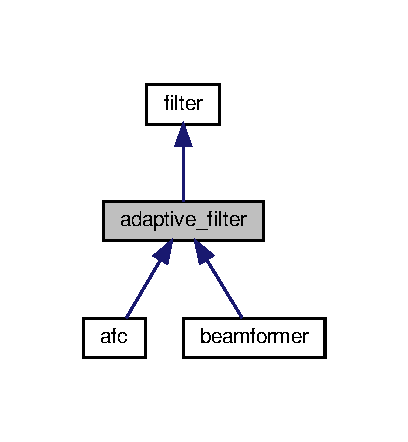
\includegraphics[width=196pt]{classadaptive__filter__inherit__graph}
\end{center}
\end{figure}


Collaboration diagram for adaptive\+\_\+filter\+:\nopagebreak
\begin{figure}[H]
\begin{center}
\leavevmode
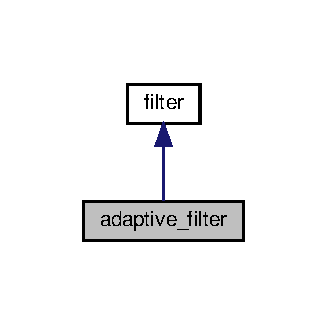
\includegraphics[width=157pt]{classadaptive__filter__coll__graph}
\end{center}
\end{figure}
\subsection*{Public Member Functions}
\begin{DoxyCompactItemize}
\item 
\hyperlink{classadaptive__filter_aacabbb2b73093c5a2e570060cff8c5c4}{adaptive\+\_\+filter} (float $\ast$adaptive\+\_\+filter\+\_\+taps, size\+\_\+t adaptive\+\_\+filter\+\_\+tap\+\_\+len, size\+\_\+t max\+\_\+frame\+\_\+size, int adaptation\+\_\+type, float mu, float delta, float rho, float alpha, float beta, float p, float c, float power\+\_\+estimate)
\begin{DoxyCompactList}\small\item\em Adaptive filter constructor. \end{DoxyCompactList}\item 
\mbox{\Hypertarget{classadaptive__filter_afca230cfdf90cd16402fc44519be3018}\label{classadaptive__filter_afca230cfdf90cd16402fc44519be3018}} 
\hyperlink{classadaptive__filter_afca230cfdf90cd16402fc44519be3018}{$\sim$adaptive\+\_\+filter} ()
\begin{DoxyCompactList}\small\item\em Adaptive filter destructor. \end{DoxyCompactList}\item 
int \hyperlink{classadaptive__filter_a5185e3472d12b41debc08e1d2c255d8e}{update\+\_\+taps} (float $\ast$u\+\_\+ref, float $\ast$e\+\_\+ref, size\+\_\+t ref\+\_\+size)
\begin{DoxyCompactList}\small\item\em To update the taps of this adaptive filter based on the reference signals u\+\_\+ref and e\+\_\+ref. \end{DoxyCompactList}\item 
size\+\_\+t \hyperlink{classadaptive__filter_a281ea01967a1e95ee3182d7be68118d7}{get\+\_\+max\+\_\+frame\+\_\+size} ()
\begin{DoxyCompactList}\small\item\em Getting the maximum frame size. \end{DoxyCompactList}\item 
void \hyperlink{classadaptive__filter_a2606c675bbd630cad6db55d77ccaa759}{get\+\_\+params} (float \&mu, float \&rho, float \&delta, float \&alpha, float \&beta, float \&p, float \&c, int \&adaptation\+\_\+type)
\begin{DoxyCompactList}\small\item\em Getting all parameters from this adaptive filter. \end{DoxyCompactList}\item 
void \hyperlink{classadaptive__filter_ad6e68bd802f05a94d37bbb9a07e221f8}{set\+\_\+params} (float mu, float rho, float delta, float alpha, float beta, float p, float c, int adaptation\+\_\+type)
\begin{DoxyCompactList}\small\item\em Setting all parameters from this adaptive filter. \end{DoxyCompactList}\end{DoxyCompactItemize}
\subsection*{Protected Member Functions}
\begin{DoxyCompactItemize}
\item 
int \hyperlink{classadaptive__filter_a5af026a803d8a024517df441304bd3e1}{get\+\_\+adaptation\+\_\+type} ()
\begin{DoxyCompactList}\small\item\em A function to get the adaptation type. \end{DoxyCompactList}\item 
void \hyperlink{classadaptive__filter_a0c14c1714918be7026d674a44969c54e}{get\+\_\+step\+\_\+size\+\_\+weights\+\_\+\+I\+P\+N\+L\+MS} (float $\ast$taps, float $\ast$step\+\_\+size\+\_\+weights, float alpha, float beta, float delta, size\+\_\+t tap\+\_\+len)
\begin{DoxyCompactList}\small\item\em A function computing the step size control matrix for I\+P\+N\+L\+M\+S-\/l\+\_\+0. \end{DoxyCompactList}\item 
void \hyperlink{classadaptive__filter_a288240ca64185c37f2e05e9ac0e812c2}{get\+\_\+step\+\_\+size\+\_\+weights\+\_\+\+S\+L\+MS} (float $\ast$taps, float $\ast$step\+\_\+size\+\_\+weights, float p, float c, size\+\_\+t tap\+\_\+len)
\begin{DoxyCompactList}\small\item\em A function computing the step size control matrix for S\+L\+MS. \end{DoxyCompactList}\end{DoxyCompactItemize}


\subsection{Detailed Description}
Adaptive Filter Class. 

This adaptive filter class implements several popular L\+M\+S-\/based algorithms including Modified L\+MS \mbox{[}Greenberg, 1998\mbox{]}, I\+P\+N\+L\+M\+S-\/l\+\_\+0 \mbox{[}Paleologu et al., 2010\mbox{]} and S\+L\+MS \mbox{[}Lee et al., 2017\mbox{]}. 

Definition at line 39 of file adaptive\+\_\+filter.\+hpp.



\subsection{Constructor \& Destructor Documentation}
\mbox{\Hypertarget{classadaptive__filter_aacabbb2b73093c5a2e570060cff8c5c4}\label{classadaptive__filter_aacabbb2b73093c5a2e570060cff8c5c4}} 
\index{adaptive\+\_\+filter@{adaptive\+\_\+filter}!adaptive\+\_\+filter@{adaptive\+\_\+filter}}
\index{adaptive\+\_\+filter@{adaptive\+\_\+filter}!adaptive\+\_\+filter@{adaptive\+\_\+filter}}
\subsubsection{\texorpdfstring{adaptive\+\_\+filter()}{adaptive\_filter()}}
{\footnotesize\ttfamily adaptive\+\_\+filter\+::adaptive\+\_\+filter (\begin{DoxyParamCaption}\item[{float $\ast$}]{adaptive\+\_\+filter\+\_\+taps,  }\item[{size\+\_\+t}]{adaptive\+\_\+filter\+\_\+tap\+\_\+len,  }\item[{size\+\_\+t}]{max\+\_\+frame\+\_\+size,  }\item[{int}]{adaptation\+\_\+type,  }\item[{float}]{mu,  }\item[{float}]{delta,  }\item[{float}]{rho,  }\item[{float}]{alpha,  }\item[{float}]{beta,  }\item[{float}]{p,  }\item[{float}]{c,  }\item[{float}]{power\+\_\+estimate }\end{DoxyParamCaption})\hspace{0.3cm}{\ttfamily [explicit]}}



Adaptive filter constructor. 


\begin{DoxyParams}[1]{Parameters}
\mbox{\tt in}  & {\em adaptive\+\_\+filter\+\_\+taps} & The initial filter taps for adaptive filter \\
\hline
\mbox{\tt in}  & {\em adaptive\+\_\+filter\+\_\+tap\+\_\+len} & The number of filter taps of adaptive filter \\
\hline
\mbox{\tt in}  & {\em max\+\_\+frame\+\_\+size} & The maximum processing frame size in adaptive filter \\
\hline
\mbox{\tt in}  & {\em adaptation\+\_\+type} & -\/1\+: 0 y\+\_\+hat, 0\+: stop adaptation, 1\+: Modified L\+MS, 2\+: I\+P\+N\+L\+M\+S-\/l\+\_\+0, 3\+: S\+L\+MS \\
\hline
\mbox{\tt in}  & {\em mu} & The gradient descent step size (learning rate) for L\+M\+S-\/based algorithms \\
\hline
\mbox{\tt in}  & {\em delta} & A small positive number to prevent dividing zero \\
\hline
\mbox{\tt in}  & {\em rho} & The forgetting factor for power estimate \\
\hline
\mbox{\tt in}  & {\em alpha} & A number between -\/1 to 1 for different degrees of sparsity in I\+P\+N\+L\+M\+S-\/l\+\_\+0 \\
\hline
\mbox{\tt in}  & {\em beta} & A number between 0 to 500 for different degrees of sparsity in I\+P\+N\+L\+M\+S-\/l\+\_\+0 \\
\hline
\mbox{\tt in}  & {\em p} & A number between 0 to 2 for fitting different degrees of sparsity in S\+L\+MS \\
\hline
\mbox{\tt in}  & {\em c} & A small positive number for preventing stagnation in S\+L\+MS \\
\hline
\mbox{\tt in}  & {\em power\+\_\+estimate} & An initial power estimate for adaptation \\
\hline
\end{DoxyParams}


Definition at line 33 of file adaptive\+\_\+filter.\+cpp.



\subsection{Member Function Documentation}
\mbox{\Hypertarget{classadaptive__filter_a5af026a803d8a024517df441304bd3e1}\label{classadaptive__filter_a5af026a803d8a024517df441304bd3e1}} 
\index{adaptive\+\_\+filter@{adaptive\+\_\+filter}!get\+\_\+adaptation\+\_\+type@{get\+\_\+adaptation\+\_\+type}}
\index{get\+\_\+adaptation\+\_\+type@{get\+\_\+adaptation\+\_\+type}!adaptive\+\_\+filter@{adaptive\+\_\+filter}}
\subsubsection{\texorpdfstring{get\+\_\+adaptation\+\_\+type()}{get\_adaptation\_type()}}
{\footnotesize\ttfamily int adaptive\+\_\+filter\+::get\+\_\+adaptation\+\_\+type (\begin{DoxyParamCaption}{ }\end{DoxyParamCaption})\hspace{0.3cm}{\ttfamily [protected]}}



A function to get the adaptation type. 

\begin{DoxyReturn}{Returns}
Adaptation type 
\end{DoxyReturn}


Definition at line 164 of file adaptive\+\_\+filter.\+cpp.

\mbox{\Hypertarget{classadaptive__filter_a281ea01967a1e95ee3182d7be68118d7}\label{classadaptive__filter_a281ea01967a1e95ee3182d7be68118d7}} 
\index{adaptive\+\_\+filter@{adaptive\+\_\+filter}!get\+\_\+max\+\_\+frame\+\_\+size@{get\+\_\+max\+\_\+frame\+\_\+size}}
\index{get\+\_\+max\+\_\+frame\+\_\+size@{get\+\_\+max\+\_\+frame\+\_\+size}!adaptive\+\_\+filter@{adaptive\+\_\+filter}}
\subsubsection{\texorpdfstring{get\+\_\+max\+\_\+frame\+\_\+size()}{get\_max\_frame\_size()}}
{\footnotesize\ttfamily size\+\_\+t adaptive\+\_\+filter\+::get\+\_\+max\+\_\+frame\+\_\+size (\begin{DoxyParamCaption}{ }\end{DoxyParamCaption})}



Getting the maximum frame size. 

\begin{DoxyReturn}{Returns}
Maximum frame size 
\end{DoxyReturn}


Definition at line 128 of file adaptive\+\_\+filter.\+cpp.

\mbox{\Hypertarget{classadaptive__filter_a2606c675bbd630cad6db55d77ccaa759}\label{classadaptive__filter_a2606c675bbd630cad6db55d77ccaa759}} 
\index{adaptive\+\_\+filter@{adaptive\+\_\+filter}!get\+\_\+params@{get\+\_\+params}}
\index{get\+\_\+params@{get\+\_\+params}!adaptive\+\_\+filter@{adaptive\+\_\+filter}}
\subsubsection{\texorpdfstring{get\+\_\+params()}{get\_params()}}
{\footnotesize\ttfamily void adaptive\+\_\+filter\+::get\+\_\+params (\begin{DoxyParamCaption}\item[{float \&}]{mu,  }\item[{float \&}]{rho,  }\item[{float \&}]{delta,  }\item[{float \&}]{alpha,  }\item[{float \&}]{beta,  }\item[{float \&}]{p,  }\item[{float \&}]{c,  }\item[{int \&}]{adaptation\+\_\+type }\end{DoxyParamCaption})}



Getting all parameters from this adaptive filter. 


\begin{DoxyParams}[1]{Parameters}
\mbox{\tt out}  & {\em mu} & The gradient descent step size (learning rate) for L\+M\+S-\/based algorithms \\
\hline
\mbox{\tt out}  & {\em rho} & The forgetting factor for power estimate \\
\hline
\mbox{\tt out}  & {\em delta} & A small positive number to prevent dividing zero \\
\hline
\mbox{\tt out}  & {\em alpha} & A number between -\/1 to 1 for different degrees of sparsity in I\+P\+N\+L\+M\+S-\/l\+\_\+0 \\
\hline
\mbox{\tt out}  & {\em beta} & A number between 0 to 500 for different degrees of sparsity in I\+P\+N\+L\+M\+S-\/l\+\_\+0 \\
\hline
\mbox{\tt out}  & {\em p} & A number between 0 to 2 for fitting different degrees of sparsity in S\+L\+MS \\
\hline
\mbox{\tt out}  & {\em c} & A small positive number for preventing stagnation in S\+L\+MS \\
\hline
\mbox{\tt out}  & {\em adaptation\+\_\+type} & -\/1\+: 0 y\+\_\+hat, 0\+: stop adaptation, 1\+: Modified L\+MS, 2\+: I\+P\+N\+L\+M\+S-\/l\+\_\+0, 3\+: S\+L\+MS \\
\hline
\end{DoxyParams}


Definition at line 133 of file adaptive\+\_\+filter.\+cpp.

\mbox{\Hypertarget{classadaptive__filter_a0c14c1714918be7026d674a44969c54e}\label{classadaptive__filter_a0c14c1714918be7026d674a44969c54e}} 
\index{adaptive\+\_\+filter@{adaptive\+\_\+filter}!get\+\_\+step\+\_\+size\+\_\+weights\+\_\+\+I\+P\+N\+L\+MS@{get\+\_\+step\+\_\+size\+\_\+weights\+\_\+\+I\+P\+N\+L\+MS}}
\index{get\+\_\+step\+\_\+size\+\_\+weights\+\_\+\+I\+P\+N\+L\+MS@{get\+\_\+step\+\_\+size\+\_\+weights\+\_\+\+I\+P\+N\+L\+MS}!adaptive\+\_\+filter@{adaptive\+\_\+filter}}
\subsubsection{\texorpdfstring{get\+\_\+step\+\_\+size\+\_\+weights\+\_\+\+I\+P\+N\+L\+M\+S()}{get\_step\_size\_weights\_IPNLMS()}}
{\footnotesize\ttfamily void adaptive\+\_\+filter\+::get\+\_\+step\+\_\+size\+\_\+weights\+\_\+\+I\+P\+N\+L\+MS (\begin{DoxyParamCaption}\item[{float $\ast$}]{taps,  }\item[{float $\ast$}]{step\+\_\+size\+\_\+weights,  }\item[{float}]{alpha,  }\item[{float}]{beta,  }\item[{float}]{delta,  }\item[{size\+\_\+t}]{tap\+\_\+len }\end{DoxyParamCaption})\hspace{0.3cm}{\ttfamily [protected]}}



A function computing the step size control matrix for I\+P\+N\+L\+M\+S-\/l\+\_\+0. 


\begin{DoxyParams}[1]{Parameters}
\mbox{\tt in}  & {\em taps} & The current filter taps of the adaptive filter \\
\hline
\mbox{\tt out}  & {\em step\+\_\+size\+\_\+weights} & The step size control matrix (it is an 1-\/D array due to the diagonal matrix) \\
\hline
\mbox{\tt in}  & {\em alpha} & A number between -\/1 to 1 for different degrees of sparsity in I\+P\+N\+L\+M\+S-\/l\+\_\+0 \\
\hline
\mbox{\tt in}  & {\em beta} & A number between 0 to 500 for different degrees of sparsity in I\+P\+N\+L\+M\+S-\/l\+\_\+0 \\
\hline
\mbox{\tt in}  & {\em delta} & A small positive number to prevent dividing zero \\
\hline
\mbox{\tt in}  & {\em tap\+\_\+len} & The number of taps of the adaptive filter \\
\hline
\end{DoxyParams}


Definition at line 170 of file adaptive\+\_\+filter.\+cpp.

\mbox{\Hypertarget{classadaptive__filter_a288240ca64185c37f2e05e9ac0e812c2}\label{classadaptive__filter_a288240ca64185c37f2e05e9ac0e812c2}} 
\index{adaptive\+\_\+filter@{adaptive\+\_\+filter}!get\+\_\+step\+\_\+size\+\_\+weights\+\_\+\+S\+L\+MS@{get\+\_\+step\+\_\+size\+\_\+weights\+\_\+\+S\+L\+MS}}
\index{get\+\_\+step\+\_\+size\+\_\+weights\+\_\+\+S\+L\+MS@{get\+\_\+step\+\_\+size\+\_\+weights\+\_\+\+S\+L\+MS}!adaptive\+\_\+filter@{adaptive\+\_\+filter}}
\subsubsection{\texorpdfstring{get\+\_\+step\+\_\+size\+\_\+weights\+\_\+\+S\+L\+M\+S()}{get\_step\_size\_weights\_SLMS()}}
{\footnotesize\ttfamily void adaptive\+\_\+filter\+::get\+\_\+step\+\_\+size\+\_\+weights\+\_\+\+S\+L\+MS (\begin{DoxyParamCaption}\item[{float $\ast$}]{taps,  }\item[{float $\ast$}]{step\+\_\+size\+\_\+weights,  }\item[{float}]{p,  }\item[{float}]{c,  }\item[{size\+\_\+t}]{tap\+\_\+len }\end{DoxyParamCaption})\hspace{0.3cm}{\ttfamily [protected]}}



A function computing the step size control matrix for S\+L\+MS. 


\begin{DoxyParams}[1]{Parameters}
\mbox{\tt in}  & {\em taps} & The current filter taps of the adaptive filter \\
\hline
\mbox{\tt out}  & {\em step\+\_\+size\+\_\+weights} & The step size control matrix (it is an 1-\/D array due to the diagonal matrix) \\
\hline
\mbox{\tt in}  & {\em p} & A number between 0 to 2 for fitting different degrees of sparsity in S\+L\+MS \\
\hline
\mbox{\tt in}  & {\em c} & A small positive number for preventing stagnation in S\+L\+MS \\
\hline
\mbox{\tt in}  & {\em tap\+\_\+len} & The number of taps of the adaptive filter \\
\hline
\end{DoxyParams}


Definition at line 184 of file adaptive\+\_\+filter.\+cpp.

\mbox{\Hypertarget{classadaptive__filter_ad6e68bd802f05a94d37bbb9a07e221f8}\label{classadaptive__filter_ad6e68bd802f05a94d37bbb9a07e221f8}} 
\index{adaptive\+\_\+filter@{adaptive\+\_\+filter}!set\+\_\+params@{set\+\_\+params}}
\index{set\+\_\+params@{set\+\_\+params}!adaptive\+\_\+filter@{adaptive\+\_\+filter}}
\subsubsection{\texorpdfstring{set\+\_\+params()}{set\_params()}}
{\footnotesize\ttfamily void adaptive\+\_\+filter\+::set\+\_\+params (\begin{DoxyParamCaption}\item[{float}]{mu,  }\item[{float}]{rho,  }\item[{float}]{delta,  }\item[{float}]{alpha,  }\item[{float}]{beta,  }\item[{float}]{p,  }\item[{float}]{c,  }\item[{int}]{adaptation\+\_\+type }\end{DoxyParamCaption})}



Setting all parameters from this adaptive filter. 


\begin{DoxyParams}[1]{Parameters}
\mbox{\tt in}  & {\em mu} & The gradient descent step size (learning rate) for L\+M\+S-\/based algorithms \\
\hline
\mbox{\tt in}  & {\em rho} & The forgetting factor for power estimate \\
\hline
\mbox{\tt in}  & {\em delta} & A small positive number to prevent dividing zero \\
\hline
\mbox{\tt in}  & {\em alpha} & A number between -\/1 to 1 for different degrees of sparsity in I\+P\+N\+L\+M\+S-\/l\+\_\+0 \\
\hline
\mbox{\tt in}  & {\em beta} & A number between 0 to 500 for different degrees of sparsity in I\+P\+N\+L\+M\+S-\/l\+\_\+0 \\
\hline
\mbox{\tt in}  & {\em p} & A number between 0 to 2 for fitting different degrees of sparsity in S\+L\+MS \\
\hline
\mbox{\tt in}  & {\em c} & A small positive number for preventing stagnation in S\+L\+MS \\
\hline
\mbox{\tt in}  & {\em adaptation\+\_\+type} & -\/1\+: 0 y\+\_\+hat, 0\+: stop adaptation, 1\+: Modified L\+MS, 2\+: I\+P\+N\+L\+M\+S-\/l\+\_\+0, 3\+: S\+L\+MS \\
\hline
\end{DoxyParams}


Definition at line 147 of file adaptive\+\_\+filter.\+cpp.

\mbox{\Hypertarget{classadaptive__filter_a5185e3472d12b41debc08e1d2c255d8e}\label{classadaptive__filter_a5185e3472d12b41debc08e1d2c255d8e}} 
\index{adaptive\+\_\+filter@{adaptive\+\_\+filter}!update\+\_\+taps@{update\+\_\+taps}}
\index{update\+\_\+taps@{update\+\_\+taps}!adaptive\+\_\+filter@{adaptive\+\_\+filter}}
\subsubsection{\texorpdfstring{update\+\_\+taps()}{update\_taps()}}
{\footnotesize\ttfamily int adaptive\+\_\+filter\+::update\+\_\+taps (\begin{DoxyParamCaption}\item[{float $\ast$}]{u\+\_\+ref,  }\item[{float $\ast$}]{e\+\_\+ref,  }\item[{size\+\_\+t}]{ref\+\_\+size }\end{DoxyParamCaption})}



To update the taps of this adaptive filter based on the reference signals u\+\_\+ref and e\+\_\+ref. 


\begin{DoxyParams}[1]{Parameters}
\mbox{\tt in}  & {\em u\+\_\+ref} & A reference input signal for adaptation \\
\hline
\mbox{\tt in}  & {\em e\+\_\+ref} & A reference error signal for adaptation \\
\hline
\mbox{\tt in}  & {\em ref\+\_\+size} & The size of each reference signal (u\+\_\+ref and e\+\_\+ref have the same size) \\
\hline
\end{DoxyParams}
\begin{DoxyReturn}{Returns}
A flag indicating the success of adaptation 
\end{DoxyReturn}


Definition at line 70 of file adaptive\+\_\+filter.\+cpp.



The documentation for this class was generated from the following files\+:\begin{DoxyCompactItemize}
\item 
\hyperlink{adaptive__filter_8hpp}{adaptive\+\_\+filter.\+hpp}\item 
\hyperlink{adaptive__filter_8cpp}{adaptive\+\_\+filter.\+cpp}\end{DoxyCompactItemize}

\hypertarget{classafc}{}\section{afc Class Reference}
\label{classafc}\index{afc@{afc}}


Adaptive Feedback Cancellation (A\+FC) Class.  




{\ttfamily \#include $<$afc.\+hpp$>$}



Inheritance diagram for afc\+:\nopagebreak
\begin{figure}[H]
\begin{center}
\leavevmode
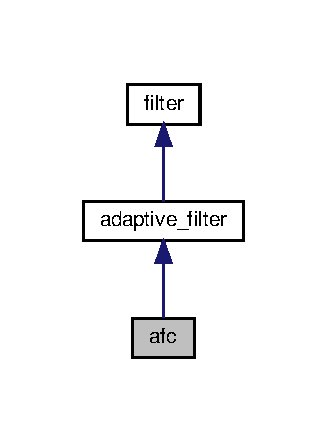
\includegraphics[width=157pt]{classafc__inherit__graph}
\end{center}
\end{figure}


Collaboration diagram for afc\+:\nopagebreak
\begin{figure}[H]
\begin{center}
\leavevmode
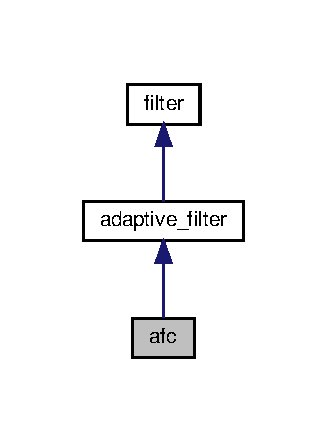
\includegraphics[width=157pt]{classafc__coll__graph}
\end{center}
\end{figure}
\subsection*{Public Member Functions}
\begin{DoxyCompactItemize}
\item 
\hyperlink{classafc_a2f6b513c6bbc373ee59b1dddcb71f6a4}{afc} (float $\ast$bandlimited\+\_\+filter\+\_\+taps, size\+\_\+t bandlimited\+\_\+filter\+\_\+tap\+\_\+len, float $\ast$prefilter\+\_\+taps, size\+\_\+t prefilter\+\_\+tap\+\_\+len, float $\ast$adaptive\+\_\+filter\+\_\+taps, size\+\_\+t adaptive\+\_\+filter\+\_\+tap\+\_\+len, size\+\_\+t max\+\_\+frame\+\_\+size, int adaptation\+\_\+type, float mu, float delta, float rho, float alpha, float beta, float p, float c, float power\+\_\+estimate, size\+\_\+t delay\+\_\+len, int afc\+\_\+on\+\_\+off)
\begin{DoxyCompactList}\small\item\em A\+FC constructor. \end{DoxyCompactList}\item 
\mbox{\Hypertarget{classafc_a9143ec3fdf33d512a307c98e977f5e5a}\label{classafc_a9143ec3fdf33d512a307c98e977f5e5a}} 
\hyperlink{classafc_a9143ec3fdf33d512a307c98e977f5e5a}{$\sim$afc} ()
\begin{DoxyCompactList}\small\item\em A\+FC destructor. \end{DoxyCompactList}\item 
int \hyperlink{classafc_ad4678623a91bce48b23dd2bdfd403682}{get\+\_\+y\+\_\+hat} (float $\ast$y\+\_\+hat, float $\ast$e, float $\ast$s, size\+\_\+t ref\+\_\+size)
\begin{DoxyCompactList}\small\item\em Getting y\+\_\+hat signal (an estimated feedback signal) \end{DoxyCompactList}\item 
void \hyperlink{classafc_abe939a99bca35b708ffd66bef80abeb4}{get\+\_\+delay} (size\+\_\+t \&delay\+\_\+len)
\begin{DoxyCompactList}\small\item\em Getting the length of delay line in samples. \end{DoxyCompactList}\item 
int \hyperlink{classafc_adf8c29b6bfc26a0d91eccdff26c76887}{set\+\_\+delay} (size\+\_\+t delay\+\_\+len)
\begin{DoxyCompactList}\small\item\em Setting the length of delay line in samples. \end{DoxyCompactList}\item 
void \hyperlink{classafc_a5e905d06e41380c61aec6221dbf203fb}{set\+\_\+afc\+\_\+on\+\_\+off} (int afc\+\_\+on\+\_\+off)
\begin{DoxyCompactList}\small\item\em Setting the O\+N/\+O\+FF for the A\+FC. \end{DoxyCompactList}\item 
void \hyperlink{classafc_a2119124c7589cb15a7b55568d5301073}{get\+\_\+afc\+\_\+on\+\_\+off} (int \&afc\+\_\+on\+\_\+off)
\begin{DoxyCompactList}\small\item\em Getting the O\+N/\+O\+FF for the A\+FC. \end{DoxyCompactList}\item 
void \hyperlink{classafc_a6f82d1ff5013e2311f099c3d4a911a75}{reset} (float $\ast$default\+\_\+taps, size\+\_\+t len)
\begin{DoxyCompactList}\small\item\em Reset the A\+FC filter to all zeros. \end{DoxyCompactList}\end{DoxyCompactItemize}
\subsection*{Additional Inherited Members}


\subsection{Detailed Description}
Adaptive Feedback Cancellation (A\+FC) Class. 

Under the F\+X\+L\+MS framework, this A\+FC class utilizes an adaptive filter to estimate the feedback signal, namely, y\+\_\+hat. 

Definition at line 40 of file afc.\+hpp.



\subsection{Constructor \& Destructor Documentation}
\mbox{\Hypertarget{classafc_a2f6b513c6bbc373ee59b1dddcb71f6a4}\label{classafc_a2f6b513c6bbc373ee59b1dddcb71f6a4}} 
\index{afc@{afc}!afc@{afc}}
\index{afc@{afc}!afc@{afc}}
\subsubsection{\texorpdfstring{afc()}{afc()}}
{\footnotesize\ttfamily afc\+::afc (\begin{DoxyParamCaption}\item[{float $\ast$}]{bandlimited\+\_\+filter\+\_\+taps,  }\item[{size\+\_\+t}]{bandlimited\+\_\+filter\+\_\+tap\+\_\+len,  }\item[{float $\ast$}]{prefilter\+\_\+taps,  }\item[{size\+\_\+t}]{prefilter\+\_\+tap\+\_\+len,  }\item[{float $\ast$}]{adaptive\+\_\+filter\+\_\+taps,  }\item[{size\+\_\+t}]{adaptive\+\_\+filter\+\_\+tap\+\_\+len,  }\item[{size\+\_\+t}]{max\+\_\+frame\+\_\+size,  }\item[{int}]{adaptation\+\_\+type,  }\item[{float}]{mu,  }\item[{float}]{delta,  }\item[{float}]{rho,  }\item[{float}]{alpha,  }\item[{float}]{beta,  }\item[{float}]{p,  }\item[{float}]{c,  }\item[{float}]{power\+\_\+estimate,  }\item[{size\+\_\+t}]{delay\+\_\+len,  }\item[{int}]{afc\+\_\+on\+\_\+off }\end{DoxyParamCaption})\hspace{0.3cm}{\ttfamily [explicit]}}



A\+FC constructor. 


\begin{DoxyParams}[1]{Parameters}
\mbox{\tt in}  & {\em bandlimited\+\_\+filter\+\_\+taps} & The filter taps for bandlimited filter in A\+FC \\
\hline
\mbox{\tt in}  & {\em bandlimited\+\_\+filter\+\_\+tap\+\_\+len} & The number of taps of bandlimited filter in A\+FC \\
\hline
\mbox{\tt in}  & {\em prefilter\+\_\+taps} & The filter taps for whitening filter in A\+FC \\
\hline
\mbox{\tt in}  & {\em prefilter\+\_\+tap\+\_\+len} & The number of taps of prefilter in A\+FC \\
\hline
\mbox{\tt in}  & {\em adaptive\+\_\+filter\+\_\+taps} & The initial filter taps for adaptive filter in A\+FC \\
\hline
\mbox{\tt in}  & {\em adaptive\+\_\+filter\+\_\+tap\+\_\+len} & The number of filter taps of adaptive filter in A\+FC \\
\hline
\mbox{\tt in}  & {\em max\+\_\+frame\+\_\+size} & The maximum processing frame size in adaptive filter \\
\hline
\mbox{\tt in}  & {\em adaptation\+\_\+type} & The adaptation type for adaptive filter \\
\hline
\mbox{\tt in}  & {\em mu} & A parameter for adaptive filter \\
\hline
\mbox{\tt in}  & {\em delta} & A parameter for adaptive filter \\
\hline
\mbox{\tt in}  & {\em rho} & A parameter for adaptive filter \\
\hline
\mbox{\tt in}  & {\em alpha} & A parameter for adaptive filter \\
\hline
\mbox{\tt in}  & {\em beta} & A parameter for adaptive filter \\
\hline
\mbox{\tt in}  & {\em p} & A parameter for adaptive filter \\
\hline
\mbox{\tt in}  & {\em c} & A parameter for adaptive filter \\
\hline
\mbox{\tt in}  & {\em power\+\_\+estimate} & A parameter for adaptive filter \\
\hline
\mbox{\tt in}  & {\em delay\+\_\+len} & The number of delay in samples \\
\hline
\mbox{\tt in}  & {\em afc\+\_\+on\+\_\+off} & A flag to turn the A\+FC on (0\+: O\+FF, 1\+: ON) \\
\hline
\end{DoxyParams}
\begin{DoxySeeAlso}{See also}
\hyperlink{classadaptive__filter}{adaptive\+\_\+filter} 
\end{DoxySeeAlso}


Definition at line 29 of file afc.\+cpp.



\subsection{Member Function Documentation}
\mbox{\Hypertarget{classafc_a2119124c7589cb15a7b55568d5301073}\label{classafc_a2119124c7589cb15a7b55568d5301073}} 
\index{afc@{afc}!get\+\_\+afc\+\_\+on\+\_\+off@{get\+\_\+afc\+\_\+on\+\_\+off}}
\index{get\+\_\+afc\+\_\+on\+\_\+off@{get\+\_\+afc\+\_\+on\+\_\+off}!afc@{afc}}
\subsubsection{\texorpdfstring{get\+\_\+afc\+\_\+on\+\_\+off()}{get\_afc\_on\_off()}}
{\footnotesize\ttfamily void afc\+::get\+\_\+afc\+\_\+on\+\_\+off (\begin{DoxyParamCaption}\item[{int \&}]{afc\+\_\+on\+\_\+off }\end{DoxyParamCaption})}



Getting the O\+N/\+O\+FF for the A\+FC. 


\begin{DoxyParams}[1]{Parameters}
\mbox{\tt in}  & {\em afc\+\_\+on\+\_\+off} & A flag indicating the O\+N/\+O\+FF of A\+FC (False\+: O\+FF, True\+: ON) \\
\hline
\end{DoxyParams}


Definition at line 120 of file afc.\+cpp.

\mbox{\Hypertarget{classafc_abe939a99bca35b708ffd66bef80abeb4}\label{classafc_abe939a99bca35b708ffd66bef80abeb4}} 
\index{afc@{afc}!get\+\_\+delay@{get\+\_\+delay}}
\index{get\+\_\+delay@{get\+\_\+delay}!afc@{afc}}
\subsubsection{\texorpdfstring{get\+\_\+delay()}{get\_delay()}}
{\footnotesize\ttfamily void afc\+::get\+\_\+delay (\begin{DoxyParamCaption}\item[{size\+\_\+t \&}]{delay\+\_\+len }\end{DoxyParamCaption})}



Getting the length of delay line in samples. 


\begin{DoxyParams}[1]{Parameters}
\mbox{\tt out}  & {\em delay\+\_\+len} & The number of delay in samples \\
\hline
\end{DoxyParams}


Definition at line 91 of file afc.\+cpp.

\mbox{\Hypertarget{classafc_ad4678623a91bce48b23dd2bdfd403682}\label{classafc_ad4678623a91bce48b23dd2bdfd403682}} 
\index{afc@{afc}!get\+\_\+y\+\_\+hat@{get\+\_\+y\+\_\+hat}}
\index{get\+\_\+y\+\_\+hat@{get\+\_\+y\+\_\+hat}!afc@{afc}}
\subsubsection{\texorpdfstring{get\+\_\+y\+\_\+hat()}{get\_y\_hat()}}
{\footnotesize\ttfamily int afc\+::get\+\_\+y\+\_\+hat (\begin{DoxyParamCaption}\item[{float $\ast$}]{y\+\_\+hat,  }\item[{float $\ast$}]{e,  }\item[{float $\ast$}]{s,  }\item[{size\+\_\+t}]{ref\+\_\+size }\end{DoxyParamCaption})}



Getting y\+\_\+hat signal (an estimated feedback signal) 


\begin{DoxyParams}[1]{Parameters}
\mbox{\tt out}  & {\em y\+\_\+hat} & An estimated feedback signal \\
\hline
\mbox{\tt in}  & {\em e} & An error signal for A\+FC (the output of hearing aid processing) \\
\hline
\mbox{\tt in}  & {\em s} & An input signal for A\+FC (the input of hearing aid processing) \\
\hline
\mbox{\tt in}  & {\em ref\+\_\+size} & The size of each signal (e and s have the same size) \\
\hline
\end{DoxyParams}
\begin{DoxyReturn}{Returns}
A flag indicating the success of getting correct y\+\_\+hat according to the adaptation type 
\end{DoxyReturn}


Definition at line 63 of file afc.\+cpp.

\mbox{\Hypertarget{classafc_a6f82d1ff5013e2311f099c3d4a911a75}\label{classafc_a6f82d1ff5013e2311f099c3d4a911a75}} 
\index{afc@{afc}!reset@{reset}}
\index{reset@{reset}!afc@{afc}}
\subsubsection{\texorpdfstring{reset()}{reset()}}
{\footnotesize\ttfamily void afc\+::reset (\begin{DoxyParamCaption}\item[{float $\ast$}]{default\+\_\+taps,  }\item[{size\+\_\+t}]{len }\end{DoxyParamCaption})}



Reset the A\+FC filter to all zeros. 


\begin{DoxyParams}[1]{Parameters}
\mbox{\tt in}  & {\em default\+\_\+taps} & The default A\+FC filter \\
\hline
\mbox{\tt in}  & {\em len} & Length of the default A\+FC filter \\
\hline
\end{DoxyParams}


Definition at line 126 of file afc.\+cpp.

\mbox{\Hypertarget{classafc_a5e905d06e41380c61aec6221dbf203fb}\label{classafc_a5e905d06e41380c61aec6221dbf203fb}} 
\index{afc@{afc}!set\+\_\+afc\+\_\+on\+\_\+off@{set\+\_\+afc\+\_\+on\+\_\+off}}
\index{set\+\_\+afc\+\_\+on\+\_\+off@{set\+\_\+afc\+\_\+on\+\_\+off}!afc@{afc}}
\subsubsection{\texorpdfstring{set\+\_\+afc\+\_\+on\+\_\+off()}{set\_afc\_on\_off()}}
{\footnotesize\ttfamily void afc\+::set\+\_\+afc\+\_\+on\+\_\+off (\begin{DoxyParamCaption}\item[{int}]{afc\+\_\+on\+\_\+off }\end{DoxyParamCaption})}



Setting the O\+N/\+O\+FF for the A\+FC. 


\begin{DoxyParams}[1]{Parameters}
\mbox{\tt in}  & {\em afc\+\_\+on\+\_\+off} & A flag to turn the A\+FC on (False\+: O\+FF, True\+: ON) \\
\hline
\end{DoxyParams}


Definition at line 111 of file afc.\+cpp.

\mbox{\Hypertarget{classafc_adf8c29b6bfc26a0d91eccdff26c76887}\label{classafc_adf8c29b6bfc26a0d91eccdff26c76887}} 
\index{afc@{afc}!set\+\_\+delay@{set\+\_\+delay}}
\index{set\+\_\+delay@{set\+\_\+delay}!afc@{afc}}
\subsubsection{\texorpdfstring{set\+\_\+delay()}{set\_delay()}}
{\footnotesize\ttfamily int afc\+::set\+\_\+delay (\begin{DoxyParamCaption}\item[{size\+\_\+t}]{delay\+\_\+len }\end{DoxyParamCaption})}



Setting the length of delay line in samples. 


\begin{DoxyParams}[1]{Parameters}
\mbox{\tt in}  & {\em delay\+\_\+len} & The number of delay in samples \\
\hline
\end{DoxyParams}
\begin{DoxyReturn}{Returns}
A flag indicating the success of setting delay\+\_\+len 
\end{DoxyReturn}


Definition at line 97 of file afc.\+cpp.



The documentation for this class was generated from the following files\+:\begin{DoxyCompactItemize}
\item 
\hyperlink{afc_8hpp}{afc.\+hpp}\item 
\hyperlink{afc_8cpp}{afc.\+cpp}\end{DoxyCompactItemize}

\hypertarget{classarray__file}{}\section{array\+\_\+file Class Reference}
\label{classarray__file}\index{array\+\_\+file@{array\+\_\+file}}


Array File Class.  




{\ttfamily \#include $<$array\+\_\+file.\+hpp$>$}

\subsection*{Public Member Functions}
\begin{DoxyCompactItemize}
\item 
\hyperlink{classarray__file_aed62743d4e948e84170eee630fb7fc99}{array\+\_\+file} (std\+::string path)
\begin{DoxyCompactList}\small\item\em Array file constructor. \end{DoxyCompactList}\item 
\mbox{\Hypertarget{classarray__file_a5101e756e2716284e64e0161ef5cdfff}\label{classarray__file_a5101e756e2716284e64e0161ef5cdfff}} 
\hyperlink{classarray__file_a5101e756e2716284e64e0161ef5cdfff}{$\sim$array\+\_\+file} ()
\begin{DoxyCompactList}\small\item\em Array file destructor. \end{DoxyCompactList}\item 
size\+\_\+t \hyperlink{classarray__file_a3add9229dd47d68e0fa4a3e2e3c5e1e1}{get\+\_\+len} ()
\begin{DoxyCompactList}\small\item\em Getting the length of the array. \end{DoxyCompactList}\item 
float $\ast$ \hyperlink{classarray__file_a5a139068e2410f90766ca94a5ab93f11}{get\+\_\+ptr} ()
\begin{DoxyCompactList}\small\item\em Getting the pointer which points to the array. \end{DoxyCompactList}\end{DoxyCompactItemize}


\subsection{Detailed Description}
Array File Class. 

Reading a binary file into an array in single-\/precision floating-\/point format 

Definition at line 33 of file array\+\_\+file.\+hpp.



\subsection{Constructor \& Destructor Documentation}
\mbox{\Hypertarget{classarray__file_aed62743d4e948e84170eee630fb7fc99}\label{classarray__file_aed62743d4e948e84170eee630fb7fc99}} 
\index{array\+\_\+file@{array\+\_\+file}!array\+\_\+file@{array\+\_\+file}}
\index{array\+\_\+file@{array\+\_\+file}!array\+\_\+file@{array\+\_\+file}}
\subsubsection{\texorpdfstring{array\+\_\+file()}{array\_file()}}
{\footnotesize\ttfamily array\+\_\+file\+::array\+\_\+file (\begin{DoxyParamCaption}\item[{std\+::string}]{path }\end{DoxyParamCaption})}



Array file constructor. 


\begin{DoxyParams}{Parameters}
{\em path} & The path of the binary file \\
\hline
\end{DoxyParams}


Definition at line 32 of file array\+\_\+file.\+cpp.



\subsection{Member Function Documentation}
\mbox{\Hypertarget{classarray__file_a3add9229dd47d68e0fa4a3e2e3c5e1e1}\label{classarray__file_a3add9229dd47d68e0fa4a3e2e3c5e1e1}} 
\index{array\+\_\+file@{array\+\_\+file}!get\+\_\+len@{get\+\_\+len}}
\index{get\+\_\+len@{get\+\_\+len}!array\+\_\+file@{array\+\_\+file}}
\subsubsection{\texorpdfstring{get\+\_\+len()}{get\_len()}}
{\footnotesize\ttfamily size\+\_\+t array\+\_\+file\+::get\+\_\+len (\begin{DoxyParamCaption}{ }\end{DoxyParamCaption})}



Getting the length of the array. 

\begin{DoxyReturn}{Returns}
The length of the array 
\end{DoxyReturn}


Definition at line 58 of file array\+\_\+file.\+cpp.

\mbox{\Hypertarget{classarray__file_a5a139068e2410f90766ca94a5ab93f11}\label{classarray__file_a5a139068e2410f90766ca94a5ab93f11}} 
\index{array\+\_\+file@{array\+\_\+file}!get\+\_\+ptr@{get\+\_\+ptr}}
\index{get\+\_\+ptr@{get\+\_\+ptr}!array\+\_\+file@{array\+\_\+file}}
\subsubsection{\texorpdfstring{get\+\_\+ptr()}{get\_ptr()}}
{\footnotesize\ttfamily float $\ast$ array\+\_\+file\+::get\+\_\+ptr (\begin{DoxyParamCaption}{ }\end{DoxyParamCaption})}



Getting the pointer which points to the array. 

\begin{DoxyReturn}{Returns}
The pointer which points to the array 
\end{DoxyReturn}


Definition at line 63 of file array\+\_\+file.\+cpp.



The documentation for this class was generated from the following files\+:\begin{DoxyCompactItemize}
\item 
\hyperlink{array__file_8hpp}{array\+\_\+file.\+hpp}\item 
\hyperlink{array__file_8cpp}{array\+\_\+file.\+cpp}\end{DoxyCompactItemize}

\hypertarget{classAudioFile}{}\section{Audio\+File$<$ T $>$ Class Template Reference}
\label{classAudioFile}\index{Audio\+File$<$ T $>$@{Audio\+File$<$ T $>$}}
\subsection*{Public Types}
\begin{DoxyCompactItemize}
\item 
\mbox{\Hypertarget{classAudioFile_ad1260a47791dc30cbabfe3ff2ea099b1}\label{classAudioFile_ad1260a47791dc30cbabfe3ff2ea099b1}} 
typedef std\+::vector$<$ std\+::vector$<$ T $>$ $>$ {\bfseries Audio\+Buffer}
\end{DoxyCompactItemize}
\subsection*{Public Member Functions}
\begin{DoxyCompactItemize}
\item 
\hyperlink{classAudioFile_ae74399e93d3f4623c7421ee10cfc0e15}{Audio\+File} ()
\item 
bool \hyperlink{classAudioFile_a0ff16123b519a4665e9f3e7d341f0a26}{load} (std\+::string file\+Path)
\item 
bool \hyperlink{classAudioFile_a415239cad5b54b4fef4a210ab79911e3}{save} (std\+::string file\+Path, \hyperlink{AudioFile_8h_ad18559d169602e85d0ad68da6ef8593f}{Audio\+File\+Format} format=Audio\+File\+Format\+::\+Wave)
\item 
uint32\+\_\+t \hyperlink{classAudioFile_a8cd1b082af9db6bd180e4a63edcdefc9}{get\+Sample\+Rate} () const
\item 
int \hyperlink{classAudioFile_a514f860a956b4494ee8d8c806391d6b3}{get\+Num\+Channels} () const
\item 
bool \hyperlink{classAudioFile_a1057326fd2c2eca7cc7937f811868cf1}{is\+Mono} () const
\item 
bool \hyperlink{classAudioFile_a380a188d95f8f23b7622dfe222a7e8f6}{is\+Stereo} () const
\item 
int \hyperlink{classAudioFile_a5495d5cb55911de54f0714e219130b48}{get\+Bit\+Depth} () const
\item 
int \hyperlink{classAudioFile_ae1b5b4b7351a79dbf810bb34ede496b9}{get\+Num\+Samples\+Per\+Channel} () const
\item 
double \hyperlink{classAudioFile_a5a6b01404675361b1c21c9c5fb5753d4}{get\+Length\+In\+Seconds} () const
\item 
void \hyperlink{classAudioFile_a7b88c68133a9ac92149c58499e026360}{print\+Summary} () const
\item 
bool \hyperlink{classAudioFile_afa0a0f7d576b0597c938c5a89746636e}{set\+Audio\+Buffer} (Audio\+Buffer \&new\+Buffer)
\item 
void \hyperlink{classAudioFile_ac155ed12db0f3b02011a7d75b525e71a}{set\+Audio\+Buffer\+Size} (int num\+Channels, int num\+Samples)
\item 
void \hyperlink{classAudioFile_a4cff9513d49e21d25de13513564784b7}{set\+Num\+Samples\+Per\+Channel} (int num\+Samples)
\item 
void \hyperlink{classAudioFile_a354018a94ae15907d7308782f2adadbb}{set\+Num\+Channels} (int num\+Channels)
\item 
void \hyperlink{classAudioFile_a2adf2ea23e7daeb8401e717c1b3d874b}{set\+Bit\+Depth} (int num\+Bits\+Per\+Sample)
\item 
void \hyperlink{classAudioFile_a2d8fa306e40535113c3eba111e16483b}{set\+Sample\+Rate} (uint32\+\_\+t new\+Sample\+Rate)
\end{DoxyCompactItemize}
\subsection*{Public Attributes}
\begin{DoxyCompactItemize}
\item 
Audio\+Buffer \hyperlink{classAudioFile_af937119db095c5af870851050dcbeabb}{samples}
\end{DoxyCompactItemize}


\subsection{Detailed Description}
\subsubsection*{template$<$class T$>$\newline
class Audio\+File$<$ T $>$}



Definition at line 47 of file Audio\+File.\+h.



\subsection{Constructor \& Destructor Documentation}
\mbox{\Hypertarget{classAudioFile_ae74399e93d3f4623c7421ee10cfc0e15}\label{classAudioFile_ae74399e93d3f4623c7421ee10cfc0e15}} 
\index{Audio\+File@{Audio\+File}!Audio\+File@{Audio\+File}}
\index{Audio\+File@{Audio\+File}!Audio\+File@{Audio\+File}}
\subsubsection{\texorpdfstring{Audio\+File()}{AudioFile()}}
{\footnotesize\ttfamily template$<$class T $>$ \\
\hyperlink{classAudioFile}{Audio\+File}$<$ T $>$\+::\hyperlink{classAudioFile}{Audio\+File} (\begin{DoxyParamCaption}{ }\end{DoxyParamCaption})}

Constructor 

Definition at line 54 of file Audio\+File.\+cpp.



\subsection{Member Function Documentation}
\mbox{\Hypertarget{classAudioFile_a5495d5cb55911de54f0714e219130b48}\label{classAudioFile_a5495d5cb55911de54f0714e219130b48}} 
\index{Audio\+File@{Audio\+File}!get\+Bit\+Depth@{get\+Bit\+Depth}}
\index{get\+Bit\+Depth@{get\+Bit\+Depth}!Audio\+File@{Audio\+File}}
\subsubsection{\texorpdfstring{get\+Bit\+Depth()}{getBitDepth()}}
{\footnotesize\ttfamily template$<$class T $>$ \\
int \hyperlink{classAudioFile}{Audio\+File}$<$ T $>$\+::get\+Bit\+Depth (\begin{DoxyParamCaption}{ }\end{DoxyParamCaption}) const}

the bit depth of each sample 

Definition at line 93 of file Audio\+File.\+cpp.

\mbox{\Hypertarget{classAudioFile_a5a6b01404675361b1c21c9c5fb5753d4}\label{classAudioFile_a5a6b01404675361b1c21c9c5fb5753d4}} 
\index{Audio\+File@{Audio\+File}!get\+Length\+In\+Seconds@{get\+Length\+In\+Seconds}}
\index{get\+Length\+In\+Seconds@{get\+Length\+In\+Seconds}!Audio\+File@{Audio\+File}}
\subsubsection{\texorpdfstring{get\+Length\+In\+Seconds()}{getLengthInSeconds()}}
{\footnotesize\ttfamily template$<$class T $>$ \\
double \hyperlink{classAudioFile}{Audio\+File}$<$ T $>$\+::get\+Length\+In\+Seconds (\begin{DoxyParamCaption}{ }\end{DoxyParamCaption}) const}

the length in seconds of the audio file based on the number of samples and sample rate 

Definition at line 110 of file Audio\+File.\+cpp.

\mbox{\Hypertarget{classAudioFile_a514f860a956b4494ee8d8c806391d6b3}\label{classAudioFile_a514f860a956b4494ee8d8c806391d6b3}} 
\index{Audio\+File@{Audio\+File}!get\+Num\+Channels@{get\+Num\+Channels}}
\index{get\+Num\+Channels@{get\+Num\+Channels}!Audio\+File@{Audio\+File}}
\subsubsection{\texorpdfstring{get\+Num\+Channels()}{getNumChannels()}}
{\footnotesize\ttfamily template$<$class T $>$ \\
int \hyperlink{classAudioFile}{Audio\+File}$<$ T $>$\+::get\+Num\+Channels (\begin{DoxyParamCaption}{ }\end{DoxyParamCaption}) const}

the number of audio channels in the buffer 

Definition at line 72 of file Audio\+File.\+cpp.

\mbox{\Hypertarget{classAudioFile_ae1b5b4b7351a79dbf810bb34ede496b9}\label{classAudioFile_ae1b5b4b7351a79dbf810bb34ede496b9}} 
\index{Audio\+File@{Audio\+File}!get\+Num\+Samples\+Per\+Channel@{get\+Num\+Samples\+Per\+Channel}}
\index{get\+Num\+Samples\+Per\+Channel@{get\+Num\+Samples\+Per\+Channel}!Audio\+File@{Audio\+File}}
\subsubsection{\texorpdfstring{get\+Num\+Samples\+Per\+Channel()}{getNumSamplesPerChannel()}}
{\footnotesize\ttfamily template$<$class T $>$ \\
int \hyperlink{classAudioFile}{Audio\+File}$<$ T $>$\+::get\+Num\+Samples\+Per\+Channel (\begin{DoxyParamCaption}{ }\end{DoxyParamCaption}) const}

the number of samples per channel 

Definition at line 100 of file Audio\+File.\+cpp.

\mbox{\Hypertarget{classAudioFile_a8cd1b082af9db6bd180e4a63edcdefc9}\label{classAudioFile_a8cd1b082af9db6bd180e4a63edcdefc9}} 
\index{Audio\+File@{Audio\+File}!get\+Sample\+Rate@{get\+Sample\+Rate}}
\index{get\+Sample\+Rate@{get\+Sample\+Rate}!Audio\+File@{Audio\+File}}
\subsubsection{\texorpdfstring{get\+Sample\+Rate()}{getSampleRate()}}
{\footnotesize\ttfamily template$<$class T $>$ \\
uint32\+\_\+t \hyperlink{classAudioFile}{Audio\+File}$<$ T $>$\+::get\+Sample\+Rate (\begin{DoxyParamCaption}{ }\end{DoxyParamCaption}) const}

the sample rate 

Definition at line 65 of file Audio\+File.\+cpp.

\mbox{\Hypertarget{classAudioFile_a1057326fd2c2eca7cc7937f811868cf1}\label{classAudioFile_a1057326fd2c2eca7cc7937f811868cf1}} 
\index{Audio\+File@{Audio\+File}!is\+Mono@{is\+Mono}}
\index{is\+Mono@{is\+Mono}!Audio\+File@{Audio\+File}}
\subsubsection{\texorpdfstring{is\+Mono()}{isMono()}}
{\footnotesize\ttfamily template$<$class T $>$ \\
bool \hyperlink{classAudioFile}{Audio\+File}$<$ T $>$\+::is\+Mono (\begin{DoxyParamCaption}{ }\end{DoxyParamCaption}) const}

true if the audio file is mono 

Definition at line 79 of file Audio\+File.\+cpp.

\mbox{\Hypertarget{classAudioFile_a380a188d95f8f23b7622dfe222a7e8f6}\label{classAudioFile_a380a188d95f8f23b7622dfe222a7e8f6}} 
\index{Audio\+File@{Audio\+File}!is\+Stereo@{is\+Stereo}}
\index{is\+Stereo@{is\+Stereo}!Audio\+File@{Audio\+File}}
\subsubsection{\texorpdfstring{is\+Stereo()}{isStereo()}}
{\footnotesize\ttfamily template$<$class T $>$ \\
bool \hyperlink{classAudioFile}{Audio\+File}$<$ T $>$\+::is\+Stereo (\begin{DoxyParamCaption}{ }\end{DoxyParamCaption}) const}

true if the audio file is stereo 

Definition at line 86 of file Audio\+File.\+cpp.

\mbox{\Hypertarget{classAudioFile_a0ff16123b519a4665e9f3e7d341f0a26}\label{classAudioFile_a0ff16123b519a4665e9f3e7d341f0a26}} 
\index{Audio\+File@{Audio\+File}!load@{load}}
\index{load@{load}!Audio\+File@{Audio\+File}}
\subsubsection{\texorpdfstring{load()}{load()}}
{\footnotesize\ttfamily template$<$class T $>$ \\
bool \hyperlink{classAudioFile}{Audio\+File}$<$ T $>$\+::load (\begin{DoxyParamCaption}\item[{std\+::string}]{file\+Path }\end{DoxyParamCaption})}

Loads an audio file from a given file path.  true if the file was successfully loaded 

Definition at line 221 of file Audio\+File.\+cpp.

\mbox{\Hypertarget{classAudioFile_a7b88c68133a9ac92149c58499e026360}\label{classAudioFile_a7b88c68133a9ac92149c58499e026360}} 
\index{Audio\+File@{Audio\+File}!print\+Summary@{print\+Summary}}
\index{print\+Summary@{print\+Summary}!Audio\+File@{Audio\+File}}
\subsubsection{\texorpdfstring{print\+Summary()}{printSummary()}}
{\footnotesize\ttfamily template$<$class T $>$ \\
void \hyperlink{classAudioFile}{Audio\+File}$<$ T $>$\+::print\+Summary (\begin{DoxyParamCaption}{ }\end{DoxyParamCaption}) const}

Prints a summary of the audio file to the console 

Definition at line 117 of file Audio\+File.\+cpp.

\mbox{\Hypertarget{classAudioFile_a415239cad5b54b4fef4a210ab79911e3}\label{classAudioFile_a415239cad5b54b4fef4a210ab79911e3}} 
\index{Audio\+File@{Audio\+File}!save@{save}}
\index{save@{save}!Audio\+File@{Audio\+File}}
\subsubsection{\texorpdfstring{save()}{save()}}
{\footnotesize\ttfamily template$<$class T $>$ \\
bool \hyperlink{classAudioFile}{Audio\+File}$<$ T $>$\+::save (\begin{DoxyParamCaption}\item[{std\+::string}]{file\+Path,  }\item[{\hyperlink{AudioFile_8h_ad18559d169602e85d0ad68da6ef8593f}{Audio\+File\+Format}}]{format = {\ttfamily AudioFileFormat\+:\+:Wave} }\end{DoxyParamCaption})}

Saves an audio file to a given file path.  true if the file was successfully saved 

Definition at line 525 of file Audio\+File.\+cpp.

\mbox{\Hypertarget{classAudioFile_afa0a0f7d576b0597c938c5a89746636e}\label{classAudioFile_afa0a0f7d576b0597c938c5a89746636e}} 
\index{Audio\+File@{Audio\+File}!set\+Audio\+Buffer@{set\+Audio\+Buffer}}
\index{set\+Audio\+Buffer@{set\+Audio\+Buffer}!Audio\+File@{Audio\+File}}
\subsubsection{\texorpdfstring{set\+Audio\+Buffer()}{setAudioBuffer()}}
{\footnotesize\ttfamily template$<$class T $>$ \\
bool \hyperlink{classAudioFile}{Audio\+File}$<$ T $>$\+::set\+Audio\+Buffer (\begin{DoxyParamCaption}\item[{Audio\+Buffer \&}]{new\+Buffer }\end{DoxyParamCaption})}

Set the audio buffer for this \hyperlink{classAudioFile}{Audio\+File} by copying samples from another buffer.  true if the buffer was copied successfully. 

Definition at line 130 of file Audio\+File.\+cpp.

\mbox{\Hypertarget{classAudioFile_ac155ed12db0f3b02011a7d75b525e71a}\label{classAudioFile_ac155ed12db0f3b02011a7d75b525e71a}} 
\index{Audio\+File@{Audio\+File}!set\+Audio\+Buffer\+Size@{set\+Audio\+Buffer\+Size}}
\index{set\+Audio\+Buffer\+Size@{set\+Audio\+Buffer\+Size}!Audio\+File@{Audio\+File}}
\subsubsection{\texorpdfstring{set\+Audio\+Buffer\+Size()}{setAudioBufferSize()}}
{\footnotesize\ttfamily template$<$class T $>$ \\
void \hyperlink{classAudioFile}{Audio\+File}$<$ T $>$\+::set\+Audio\+Buffer\+Size (\begin{DoxyParamCaption}\item[{int}]{num\+Channels,  }\item[{int}]{num\+Samples }\end{DoxyParamCaption})}

Sets the audio buffer to a given number of channels and number of samples per channel. This will try to preserve the existing audio, adding zeros to any new channels or new samples in a given channel. 

Definition at line 162 of file Audio\+File.\+cpp.

\mbox{\Hypertarget{classAudioFile_a2adf2ea23e7daeb8401e717c1b3d874b}\label{classAudioFile_a2adf2ea23e7daeb8401e717c1b3d874b}} 
\index{Audio\+File@{Audio\+File}!set\+Bit\+Depth@{set\+Bit\+Depth}}
\index{set\+Bit\+Depth@{set\+Bit\+Depth}!Audio\+File@{Audio\+File}}
\subsubsection{\texorpdfstring{set\+Bit\+Depth()}{setBitDepth()}}
{\footnotesize\ttfamily template$<$class T $>$ \\
void \hyperlink{classAudioFile}{Audio\+File}$<$ T $>$\+::set\+Bit\+Depth (\begin{DoxyParamCaption}\item[{int}]{num\+Bits\+Per\+Sample }\end{DoxyParamCaption})}

Sets the bit depth for the audio file. If you use the \hyperlink{classAudioFile_a415239cad5b54b4fef4a210ab79911e3}{save()} function, this bit depth rate will be used 

Definition at line 207 of file Audio\+File.\+cpp.

\mbox{\Hypertarget{classAudioFile_a354018a94ae15907d7308782f2adadbb}\label{classAudioFile_a354018a94ae15907d7308782f2adadbb}} 
\index{Audio\+File@{Audio\+File}!set\+Num\+Channels@{set\+Num\+Channels}}
\index{set\+Num\+Channels@{set\+Num\+Channels}!Audio\+File@{Audio\+File}}
\subsubsection{\texorpdfstring{set\+Num\+Channels()}{setNumChannels()}}
{\footnotesize\ttfamily template$<$class T $>$ \\
void \hyperlink{classAudioFile}{Audio\+File}$<$ T $>$\+::set\+Num\+Channels (\begin{DoxyParamCaption}\item[{int}]{num\+Channels }\end{DoxyParamCaption})}

Sets the number of channels. New channels will have the correct number of samples and be initialised to zero 

Definition at line 186 of file Audio\+File.\+cpp.

\mbox{\Hypertarget{classAudioFile_a4cff9513d49e21d25de13513564784b7}\label{classAudioFile_a4cff9513d49e21d25de13513564784b7}} 
\index{Audio\+File@{Audio\+File}!set\+Num\+Samples\+Per\+Channel@{set\+Num\+Samples\+Per\+Channel}}
\index{set\+Num\+Samples\+Per\+Channel@{set\+Num\+Samples\+Per\+Channel}!Audio\+File@{Audio\+File}}
\subsubsection{\texorpdfstring{set\+Num\+Samples\+Per\+Channel()}{setNumSamplesPerChannel()}}
{\footnotesize\ttfamily template$<$class T $>$ \\
void \hyperlink{classAudioFile}{Audio\+File}$<$ T $>$\+::set\+Num\+Samples\+Per\+Channel (\begin{DoxyParamCaption}\item[{int}]{num\+Samples }\end{DoxyParamCaption})}

Sets the number of samples per channel in the audio buffer. This will try to preserve the existing audio, adding zeros to new samples in a given channel if the number of samples is increased. 

Definition at line 170 of file Audio\+File.\+cpp.

\mbox{\Hypertarget{classAudioFile_a2d8fa306e40535113c3eba111e16483b}\label{classAudioFile_a2d8fa306e40535113c3eba111e16483b}} 
\index{Audio\+File@{Audio\+File}!set\+Sample\+Rate@{set\+Sample\+Rate}}
\index{set\+Sample\+Rate@{set\+Sample\+Rate}!Audio\+File@{Audio\+File}}
\subsubsection{\texorpdfstring{set\+Sample\+Rate()}{setSampleRate()}}
{\footnotesize\ttfamily template$<$class T $>$ \\
void \hyperlink{classAudioFile}{Audio\+File}$<$ T $>$\+::set\+Sample\+Rate (\begin{DoxyParamCaption}\item[{uint32\+\_\+t}]{new\+Sample\+Rate }\end{DoxyParamCaption})}

Sets the sample rate for the audio file. If you use the \hyperlink{classAudioFile_a415239cad5b54b4fef4a210ab79911e3}{save()} function, this sample rate will be used 

Definition at line 214 of file Audio\+File.\+cpp.



\subsection{Member Data Documentation}
\mbox{\Hypertarget{classAudioFile_af937119db095c5af870851050dcbeabb}\label{classAudioFile_af937119db095c5af870851050dcbeabb}} 
\index{Audio\+File@{Audio\+File}!samples@{samples}}
\index{samples@{samples}!Audio\+File@{Audio\+File}}
\subsubsection{\texorpdfstring{samples}{samples}}
{\footnotesize\ttfamily template$<$class T$>$ \\
Audio\+Buffer \hyperlink{classAudioFile}{Audio\+File}$<$ T $>$\+::samples}

A vector of vectors holding the audio samples for the \hyperlink{classAudioFile}{Audio\+File}. You can access the samples by channel and then by sample index, i.\+e\+: \begin{DoxyVerb} samples[channel][sampleIndex]\end{DoxyVerb}
 

Definition at line 126 of file Audio\+File.\+h.



The documentation for this class was generated from the following files\+:\begin{DoxyCompactItemize}
\item 
\hyperlink{AudioFile_8h}{Audio\+File.\+h}\item 
\hyperlink{AudioFile_8cpp}{Audio\+File.\+cpp}\end{DoxyCompactItemize}

\hypertarget{classbeamformer}{}\section{beamformer Class Reference}
\label{classbeamformer}\index{beamformer@{beamformer}}


Beamformer Class.  




{\ttfamily \#include $<$beamformer.\+hpp$>$}



Inheritance diagram for beamformer\+:\nopagebreak
\begin{figure}[H]
\begin{center}
\leavevmode
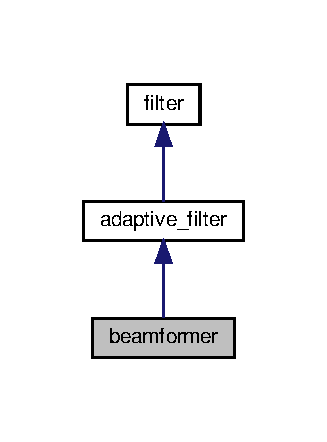
\includegraphics[width=157pt]{classbeamformer__inherit__graph}
\end{center}
\end{figure}


Collaboration diagram for beamformer\+:\nopagebreak
\begin{figure}[H]
\begin{center}
\leavevmode
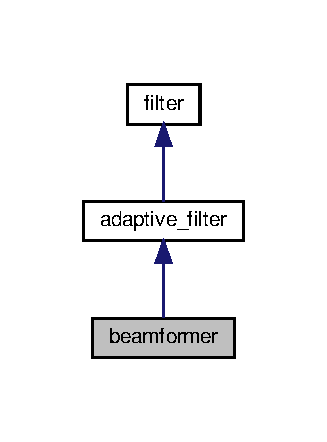
\includegraphics[width=157pt]{classbeamformer__coll__graph}
\end{center}
\end{figure}
\subsection*{Public Member Functions}
\begin{DoxyCompactItemize}
\item 
\hyperlink{classbeamformer_a30c14263a887cada41e51dffd39991c8}{beamformer} (size\+\_\+t delay\+\_\+len, float $\ast$adaptive\+\_\+filter\+\_\+taps, size\+\_\+t adaptive\+\_\+filter\+\_\+tap\+\_\+len, size\+\_\+t max\+\_\+frame\+\_\+size, int adaptation\+\_\+type, float mu, float delta, float rho, float alpha, float beta, float p, float c, float power\+\_\+estimate, int bf\+\_\+on\+\_\+off, int bf\+\_\+nc\+\_\+on\+\_\+off, int bf\+\_\+amc\+\_\+on\+\_\+off, float nc\+\_\+thr, float amc\+\_\+thr, float amc\+\_\+forgetting\+\_\+factor)
\begin{DoxyCompactList}\small\item\em Beamformer constructor. \end{DoxyCompactList}\item 
\mbox{\Hypertarget{classbeamformer_abedc8820adb8711f5fe9f9786bdcbcbf}\label{classbeamformer_abedc8820adb8711f5fe9f9786bdcbcbf}} 
\hyperlink{classbeamformer_abedc8820adb8711f5fe9f9786bdcbcbf}{$\sim$beamformer} ()
\begin{DoxyCompactList}\small\item\em Beamformer destructor. \end{DoxyCompactList}\item 
void \hyperlink{classbeamformer_a557285c2c9ba3cc59cb73db8e5e823ed}{get\+\_\+e} (float $\ast$e\+\_\+l, float $\ast$e\+\_\+r, const float $\ast$x\+\_\+l, const float $\ast$x\+\_\+r, size\+\_\+t ref\+\_\+size)
\begin{DoxyCompactList}\small\item\em Getting e signal (the output signal of this beamformer) \end{DoxyCompactList}\item 
int \hyperlink{classbeamformer_a5c98a192f70faf7dc3f354f677bec4ee}{update\+\_\+bf\+\_\+taps} (size\+\_\+t ref\+\_\+size)
\begin{DoxyCompactList}\small\item\em Update the taps of the beamformer. \end{DoxyCompactList}\item 
void \hyperlink{classbeamformer_af3f89821c2cd4e52a9ed634d0d73aa3a}{get\+\_\+bf\+\_\+params} (int \&bf\+\_\+on\+\_\+off, int \&bf\+\_\+nc\+\_\+on\+\_\+off, int \&bf\+\_\+amc\+\_\+on\+\_\+off, float \&nc\+\_\+thr, float \&amc\+\_\+thr, float \&amc\+\_\+forgetting\+\_\+factor)
\begin{DoxyCompactList}\small\item\em Getting all parameters from this beamformer. \end{DoxyCompactList}\item 
void \hyperlink{classbeamformer_ac608a617588757dba3ac80c88a3d3c70}{set\+\_\+bf\+\_\+params} (int bf\+\_\+on\+\_\+off, int bf\+\_\+nc\+\_\+on\+\_\+off, int bf\+\_\+amc\+\_\+on\+\_\+off, float nc\+\_\+thr, float amc\+\_\+thr, float amc\+\_\+forgetting\+\_\+factor)
\begin{DoxyCompactList}\small\item\em Setting all parameters from this beamformer. \end{DoxyCompactList}\end{DoxyCompactItemize}
\subsection*{Additional Inherited Members}


\subsection{Detailed Description}
Beamformer Class. 

This beamformer class implements the generalized sidelobe canceller (G\+SC) using S\+L\+MS \mbox{[}Lee et al., I\+H\+C\+ON 2018\mbox{]}. 

Definition at line 39 of file beamformer.\+hpp.



\subsection{Constructor \& Destructor Documentation}
\mbox{\Hypertarget{classbeamformer_a30c14263a887cada41e51dffd39991c8}\label{classbeamformer_a30c14263a887cada41e51dffd39991c8}} 
\index{beamformer@{beamformer}!beamformer@{beamformer}}
\index{beamformer@{beamformer}!beamformer@{beamformer}}
\subsubsection{\texorpdfstring{beamformer()}{beamformer()}}
{\footnotesize\ttfamily beamformer\+::beamformer (\begin{DoxyParamCaption}\item[{size\+\_\+t}]{delay\+\_\+len,  }\item[{float $\ast$}]{adaptive\+\_\+filter\+\_\+taps,  }\item[{size\+\_\+t}]{adaptive\+\_\+filter\+\_\+tap\+\_\+len,  }\item[{size\+\_\+t}]{max\+\_\+frame\+\_\+size,  }\item[{int}]{adaptation\+\_\+type,  }\item[{float}]{mu,  }\item[{float}]{delta,  }\item[{float}]{rho,  }\item[{float}]{alpha,  }\item[{float}]{beta,  }\item[{float}]{p,  }\item[{float}]{c,  }\item[{float}]{power\+\_\+estimate,  }\item[{int}]{bf\+\_\+on\+\_\+off,  }\item[{int}]{bf\+\_\+nc\+\_\+on\+\_\+off,  }\item[{int}]{bf\+\_\+amc\+\_\+on\+\_\+off,  }\item[{float}]{nc\+\_\+thr,  }\item[{float}]{amc\+\_\+thr,  }\item[{float}]{amc\+\_\+forgetting\+\_\+factor }\end{DoxyParamCaption})\hspace{0.3cm}{\ttfamily [explicit]}}



Beamformer constructor. 


\begin{DoxyParams}[1]{Parameters}
\mbox{\tt in}  & {\em delay\+\_\+len} & The length of delay line in samples for beamformer \\
\hline
\mbox{\tt in}  & {\em adaptive\+\_\+filter\+\_\+taps} & The initial filter taps for adaptive filter in beamformer \\
\hline
\mbox{\tt in}  & {\em adaptive\+\_\+filter\+\_\+tap\+\_\+len} & The number of filter taps of adaptive filter in beamformer \\
\hline
\mbox{\tt in}  & {\em max\+\_\+frame\+\_\+size} & The maximum processing frame size in adaptive filter \\
\hline
\mbox{\tt in}  & {\em adaptation\+\_\+type} & The adaptation type for adaptive filter \\
\hline
\mbox{\tt in}  & {\em mu} & A parameter for adaptive filter \\
\hline
\mbox{\tt in}  & {\em delta} & A parameter for adaptive filter \\
\hline
\mbox{\tt in}  & {\em rho} & A parameter for adaptive filter \\
\hline
\mbox{\tt in}  & {\em alpha} & A parameter for adaptive filter \\
\hline
\mbox{\tt in}  & {\em beta} & A parameter for adaptive filter \\
\hline
\mbox{\tt in}  & {\em p} & A parameter for adaptive filter \\
\hline
\mbox{\tt in}  & {\em c} & A parameter for adaptive filter \\
\hline
\mbox{\tt in}  & {\em power\+\_\+estimate} & A parameter for adaptive filter \\
\hline
\mbox{\tt in}  & {\em bf\+\_\+on\+\_\+off} & A flag for enabling beamformer \\
\hline
\mbox{\tt in}  & {\em bf\+\_\+nc\+\_\+on\+\_\+off} & A flag for enabling norm-\/constrained adaptation \\
\hline
\mbox{\tt in}  & {\em bf\+\_\+amc\+\_\+on\+\_\+off} & A flag for enabling adaptation mode controller \\
\hline
\mbox{\tt in}  & {\em nc\+\_\+thr} & A threshold for the norm-\/constrained adaptation \\
\hline
\mbox{\tt in}  & {\em amc\+\_\+thr} & A threshold for the adaptation mode controller \\
\hline
\end{DoxyParams}
\begin{DoxySeeAlso}{See also}
\hyperlink{classadaptive__filter}{adaptive\+\_\+filter} 
\end{DoxySeeAlso}


Definition at line 32 of file beamformer.\+cpp.



\subsection{Member Function Documentation}
\mbox{\Hypertarget{classbeamformer_af3f89821c2cd4e52a9ed634d0d73aa3a}\label{classbeamformer_af3f89821c2cd4e52a9ed634d0d73aa3a}} 
\index{beamformer@{beamformer}!get\+\_\+bf\+\_\+params@{get\+\_\+bf\+\_\+params}}
\index{get\+\_\+bf\+\_\+params@{get\+\_\+bf\+\_\+params}!beamformer@{beamformer}}
\subsubsection{\texorpdfstring{get\+\_\+bf\+\_\+params()}{get\_bf\_params()}}
{\footnotesize\ttfamily void beamformer\+::get\+\_\+bf\+\_\+params (\begin{DoxyParamCaption}\item[{int \&}]{bf\+\_\+on\+\_\+off,  }\item[{int \&}]{bf\+\_\+nc\+\_\+on\+\_\+off,  }\item[{int \&}]{bf\+\_\+amc\+\_\+on\+\_\+off,  }\item[{float \&}]{nc\+\_\+thr,  }\item[{float \&}]{amc\+\_\+thr,  }\item[{float \&}]{amc\+\_\+forgetting\+\_\+factor }\end{DoxyParamCaption})}



Getting all parameters from this beamformer. 


\begin{DoxyParams}[1]{Parameters}
\mbox{\tt out}  & {\em bf\+\_\+on\+\_\+off} & A flag to turn the beamformer on (0\+: O\+FF, 1\+: ON) \\
\hline
\mbox{\tt out}  & {\em bf\+\_\+nc\+\_\+on\+\_\+off} & A flag to turn the norm-\/constrained adaptation on (0\+: O\+FF, 1\+: ON) \\
\hline
\mbox{\tt out}  & {\em bf\+\_\+amc\+\_\+on\+\_\+off} & A flag to turn the adaptation mode controller on (0\+: O\+FF, 1\+: ON) \\
\hline
\mbox{\tt out}  & {\em nc\+\_\+thr} & A threshold for the norm-\/constrained adaptation \\
\hline
\mbox{\tt out}  & {\em amc\+\_\+thr} & A threshold for the adaptation mode controller \\
\hline
\mbox{\tt out}  & {\em amc\+\_\+forgetting\+\_\+factor} & A forgetting factor to compute the signal power \\
\hline
\end{DoxyParams}


Definition at line 142 of file beamformer.\+cpp.

\mbox{\Hypertarget{classbeamformer_a557285c2c9ba3cc59cb73db8e5e823ed}\label{classbeamformer_a557285c2c9ba3cc59cb73db8e5e823ed}} 
\index{beamformer@{beamformer}!get\+\_\+e@{get\+\_\+e}}
\index{get\+\_\+e@{get\+\_\+e}!beamformer@{beamformer}}
\subsubsection{\texorpdfstring{get\+\_\+e()}{get\_e()}}
{\footnotesize\ttfamily void beamformer\+::get\+\_\+e (\begin{DoxyParamCaption}\item[{float $\ast$}]{e\+\_\+l,  }\item[{float $\ast$}]{e\+\_\+r,  }\item[{const float $\ast$}]{x\+\_\+l,  }\item[{const float $\ast$}]{x\+\_\+r,  }\item[{size\+\_\+t}]{ref\+\_\+size }\end{DoxyParamCaption})}



Getting e signal (the output signal of this beamformer) 


\begin{DoxyParams}[1]{Parameters}
\mbox{\tt out}  & {\em e\+\_\+l} & The output signal of this beamformer on the left \\
\hline
\mbox{\tt out}  & {\em e\+\_\+r} & The output signal of this beamformer on the right \\
\hline
\mbox{\tt in}  & {\em x\+\_\+l} & The input signal from the left channel \\
\hline
\mbox{\tt in}  & {\em x\+\_\+r} & the input signal from the right channel \\
\hline
\mbox{\tt in}  & {\em ref\+\_\+size} & The size of each input signal (x\+\_\+l and x\+\_\+r have the same size) \\
\hline
\end{DoxyParams}


Definition at line 70 of file beamformer.\+cpp.

\mbox{\Hypertarget{classbeamformer_ac608a617588757dba3ac80c88a3d3c70}\label{classbeamformer_ac608a617588757dba3ac80c88a3d3c70}} 
\index{beamformer@{beamformer}!set\+\_\+bf\+\_\+params@{set\+\_\+bf\+\_\+params}}
\index{set\+\_\+bf\+\_\+params@{set\+\_\+bf\+\_\+params}!beamformer@{beamformer}}
\subsubsection{\texorpdfstring{set\+\_\+bf\+\_\+params()}{set\_bf\_params()}}
{\footnotesize\ttfamily void beamformer\+::set\+\_\+bf\+\_\+params (\begin{DoxyParamCaption}\item[{int}]{bf\+\_\+on\+\_\+off,  }\item[{int}]{bf\+\_\+nc\+\_\+on\+\_\+off,  }\item[{int}]{bf\+\_\+amc\+\_\+on\+\_\+off,  }\item[{float}]{nc\+\_\+thr,  }\item[{float}]{amc\+\_\+thr,  }\item[{float}]{amc\+\_\+forgetting\+\_\+factor }\end{DoxyParamCaption})}



Setting all parameters from this beamformer. 


\begin{DoxyParams}[1]{Parameters}
\mbox{\tt in}  & {\em bf\+\_\+on\+\_\+off} & A flag to turn the beamformer on (0\+: O\+FF, 1\+: ON) \\
\hline
\mbox{\tt in}  & {\em bf\+\_\+nc\+\_\+on\+\_\+off} & A flag to turn the norm-\/constrained adaptation on (0\+: O\+FF, 1\+: ON) \\
\hline
\mbox{\tt in}  & {\em bf\+\_\+amc\+\_\+on\+\_\+off} & A flag to turn the adaptation mode controller on (0\+: O\+FF, 1\+: ON) \\
\hline
\mbox{\tt in}  & {\em nc\+\_\+thr} & A threshold for the norm-\/constrained adaptation \\
\hline
\mbox{\tt in}  & {\em amc\+\_\+thr} & A threshold for the adaptation mode controller \\
\hline
\mbox{\tt in}  & {\em amc\+\_\+forgetting\+\_\+factor} & A forgetting factor to compute the signal power \\
\hline
\end{DoxyParams}


Definition at line 153 of file beamformer.\+cpp.

\mbox{\Hypertarget{classbeamformer_a5c98a192f70faf7dc3f354f677bec4ee}\label{classbeamformer_a5c98a192f70faf7dc3f354f677bec4ee}} 
\index{beamformer@{beamformer}!update\+\_\+bf\+\_\+taps@{update\+\_\+bf\+\_\+taps}}
\index{update\+\_\+bf\+\_\+taps@{update\+\_\+bf\+\_\+taps}!beamformer@{beamformer}}
\subsubsection{\texorpdfstring{update\+\_\+bf\+\_\+taps()}{update\_bf\_taps()}}
{\footnotesize\ttfamily int beamformer\+::update\+\_\+bf\+\_\+taps (\begin{DoxyParamCaption}\item[{size\+\_\+t}]{ref\+\_\+size }\end{DoxyParamCaption})}



Update the taps of the beamformer. 


\begin{DoxyParams}[1]{Parameters}
\mbox{\tt in}  & {\em ref\+\_\+size} & The size of each input signal (x\+\_\+l and x\+\_\+r have the same size) \\
\hline
\end{DoxyParams}
\begin{DoxyReturn}{Returns}
A flag indicating the success of adaptation in adaptive filter 
\end{DoxyReturn}


Definition at line 102 of file beamformer.\+cpp.



The documentation for this class was generated from the following files\+:\begin{DoxyCompactItemize}
\item 
\hyperlink{beamformer_8hpp}{beamformer.\+hpp}\item 
\hyperlink{beamformer_8cpp}{beamformer.\+cpp}\end{DoxyCompactItemize}

\hypertarget{classcircular__buffer}{}\section{circular\+\_\+buffer Class Reference}
\label{classcircular__buffer}\index{circular\+\_\+buffer@{circular\+\_\+buffer}}


Circular Buffer Class.  




{\ttfamily \#include $<$circular\+\_\+buffer.\+hpp$>$}

\subsection*{Public Member Functions}
\begin{DoxyCompactItemize}
\item 
\hyperlink{classcircular__buffer_a7be48ff2159478cb59111c7f0e888799}{circular\+\_\+buffer} (size\+\_\+t \hyperlink{classcircular__buffer_ae8fb2f8eb0275b98b6767d5e3979787a}{size}, float \hyperlink{classcircular__buffer_a36426e279d80a1616fb858582eae3f1f}{reset})
\begin{DoxyCompactList}\small\item\em Circular buffer constructor. \end{DoxyCompactList}\item 
\mbox{\Hypertarget{classcircular__buffer_af63809aa67a0ab961bfddb5a143b3a74}\label{classcircular__buffer_af63809aa67a0ab961bfddb5a143b3a74}} 
\hyperlink{classcircular__buffer_af63809aa67a0ab961bfddb5a143b3a74}{$\sim$circular\+\_\+buffer} ()
\begin{DoxyCompactList}\small\item\em Default destructor. \end{DoxyCompactList}\item 
void \hyperlink{classcircular__buffer_a0b2b66f74f1e588ed452caaf8cbbbe8e}{set} (const float $\ast$item, size\+\_\+t buf\+\_\+size)
\begin{DoxyCompactList}\small\item\em This is the set command for the circular buffer. \end{DoxyCompactList}\item 
void \hyperlink{classcircular__buffer_a98ceb4a6a8a321dec5f4ad6fb70e3ca6}{get} (float $\ast$data, size\+\_\+t buf\+\_\+size)
\begin{DoxyCompactList}\small\item\em This is the get function for the circular buffer. \end{DoxyCompactList}\item 
void \hyperlink{classcircular__buffer_a39828678a4debfd0ce70196260f62956}{delay\+\_\+block} (float $\ast$data, size\+\_\+t buf\+\_\+size, size\+\_\+t delay)
\begin{DoxyCompactList}\small\item\em This is the get function for the circular buffer with a delay. \end{DoxyCompactList}\item 
\mbox{\Hypertarget{classcircular__buffer_a36426e279d80a1616fb858582eae3f1f}\label{classcircular__buffer_a36426e279d80a1616fb858582eae3f1f}} 
void \hyperlink{classcircular__buffer_a36426e279d80a1616fb858582eae3f1f}{reset} ()
\begin{DoxyCompactList}\small\item\em This is the reset command for circular buffer. It resets all of the values in the buffer to the default value the user entered in the constructor. \end{DoxyCompactList}\item 
size\+\_\+t \hyperlink{classcircular__buffer_ae8fb2f8eb0275b98b6767d5e3979787a}{size} () const
\begin{DoxyCompactList}\small\item\em Function to get the size of the buffer. \end{DoxyCompactList}\end{DoxyCompactItemize}
\subsection*{Public Attributes}
\begin{DoxyCompactItemize}
\item 
\mbox{\Hypertarget{classcircular__buffer_a14ef6a352fc8ba6a5f5ba3ef79579b35}\label{classcircular__buffer_a14ef6a352fc8ba6a5f5ba3ef79579b35}} 
float $\ast$ {\bfseries buf\+\_\+}
\item 
\mbox{\Hypertarget{classcircular__buffer_ae0840d62ae876718d65854e9f3478b6f}\label{classcircular__buffer_ae0840d62ae876718d65854e9f3478b6f}} 
std\+::atomic$<$ size\+\_\+t $>$ {\bfseries head\+\_\+}
\item 
\mbox{\Hypertarget{classcircular__buffer_ac405641287665aceb64d65c99b00abc9}\label{classcircular__buffer_ac405641287665aceb64d65c99b00abc9}} 
size\+\_\+t {\bfseries size\+\_\+}
\item 
\mbox{\Hypertarget{classcircular__buffer_a3733cb9af9b280d0277d6337857e3e72}\label{classcircular__buffer_a3733cb9af9b280d0277d6337857e3e72}} 
size\+\_\+t {\bfseries mask\+\_\+}
\item 
\mbox{\Hypertarget{classcircular__buffer_a2ad9096ce4ecd7e86997c3f471e7a10e}\label{classcircular__buffer_a2ad9096ce4ecd7e86997c3f471e7a10e}} 
float {\bfseries reset\+\_\+}
\end{DoxyCompactItemize}


\subsection{Detailed Description}
Circular Buffer Class. 

Definition at line 36 of file circular\+\_\+buffer.\+hpp.



\subsection{Constructor \& Destructor Documentation}
\mbox{\Hypertarget{classcircular__buffer_a7be48ff2159478cb59111c7f0e888799}\label{classcircular__buffer_a7be48ff2159478cb59111c7f0e888799}} 
\index{circular\+\_\+buffer@{circular\+\_\+buffer}!circular\+\_\+buffer@{circular\+\_\+buffer}}
\index{circular\+\_\+buffer@{circular\+\_\+buffer}!circular\+\_\+buffer@{circular\+\_\+buffer}}
\subsubsection{\texorpdfstring{circular\+\_\+buffer()}{circular\_buffer()}}
{\footnotesize\ttfamily circular\+\_\+buffer\+::circular\+\_\+buffer (\begin{DoxyParamCaption}\item[{size\+\_\+t}]{size,  }\item[{float}]{reset }\end{DoxyParamCaption})\hspace{0.3cm}{\ttfamily [explicit]}}



Circular buffer constructor. 


\begin{DoxyParams}[1]{Parameters}
\mbox{\tt in}  & {\em size} & The maximum size you would want your circular buffer to be \\
\hline
\mbox{\tt in}  & {\em reset} & The value you want to reset all of the values in the circular buffer to \\
\hline
\end{DoxyParams}


Definition at line 34 of file circular\+\_\+buffer.\+cpp.



\subsection{Member Function Documentation}
\mbox{\Hypertarget{classcircular__buffer_a39828678a4debfd0ce70196260f62956}\label{classcircular__buffer_a39828678a4debfd0ce70196260f62956}} 
\index{circular\+\_\+buffer@{circular\+\_\+buffer}!delay\+\_\+block@{delay\+\_\+block}}
\index{delay\+\_\+block@{delay\+\_\+block}!circular\+\_\+buffer@{circular\+\_\+buffer}}
\subsubsection{\texorpdfstring{delay\+\_\+block()}{delay\_block()}}
{\footnotesize\ttfamily void circular\+\_\+buffer\+::delay\+\_\+block (\begin{DoxyParamCaption}\item[{float $\ast$}]{data,  }\item[{size\+\_\+t}]{buf\+\_\+size,  }\item[{size\+\_\+t}]{delay }\end{DoxyParamCaption})}



This is the get function for the circular buffer with a delay. 


\begin{DoxyParams}[1]{Parameters}
\mbox{\tt out}  & {\em data} & A buffer to put your data in. \\
\hline
\mbox{\tt in}  & {\em buf\+\_\+size} & The amount of data you want from the circular buffer \\
\hline
\mbox{\tt in}  & {\em delay} & The delay you want form the delay block in terms of time step \\
\hline
\end{DoxyParams}


Definition at line 87 of file circular\+\_\+buffer.\+cpp.

\mbox{\Hypertarget{classcircular__buffer_a98ceb4a6a8a321dec5f4ad6fb70e3ca6}\label{classcircular__buffer_a98ceb4a6a8a321dec5f4ad6fb70e3ca6}} 
\index{circular\+\_\+buffer@{circular\+\_\+buffer}!get@{get}}
\index{get@{get}!circular\+\_\+buffer@{circular\+\_\+buffer}}
\subsubsection{\texorpdfstring{get()}{get()}}
{\footnotesize\ttfamily void circular\+\_\+buffer\+::get (\begin{DoxyParamCaption}\item[{float $\ast$}]{data,  }\item[{size\+\_\+t}]{buf\+\_\+size }\end{DoxyParamCaption})}



This is the get function for the circular buffer. 


\begin{DoxyParams}[1]{Parameters}
\mbox{\tt out}  & {\em data} & A buffer to put your data in. \\
\hline
\mbox{\tt in}  & {\em buf\+\_\+size} & The amount of data you want from the circular buffer \\
\hline
\end{DoxyParams}


Definition at line 71 of file circular\+\_\+buffer.\+cpp.

\mbox{\Hypertarget{classcircular__buffer_a0b2b66f74f1e588ed452caaf8cbbbe8e}\label{classcircular__buffer_a0b2b66f74f1e588ed452caaf8cbbbe8e}} 
\index{circular\+\_\+buffer@{circular\+\_\+buffer}!set@{set}}
\index{set@{set}!circular\+\_\+buffer@{circular\+\_\+buffer}}
\subsubsection{\texorpdfstring{set()}{set()}}
{\footnotesize\ttfamily void circular\+\_\+buffer\+::set (\begin{DoxyParamCaption}\item[{const float $\ast$}]{item,  }\item[{size\+\_\+t}]{buf\+\_\+size }\end{DoxyParamCaption})}



This is the set command for the circular buffer. 


\begin{DoxyParams}[1]{Parameters}
\mbox{\tt in}  & {\em item} & The buffer of data you want to put in the circular buffer \\
\hline
\mbox{\tt in}  & {\em buf\+\_\+size} & The size of the buffer. \\
\hline
\end{DoxyParams}


Definition at line 52 of file circular\+\_\+buffer.\+cpp.

\mbox{\Hypertarget{classcircular__buffer_ae8fb2f8eb0275b98b6767d5e3979787a}\label{classcircular__buffer_ae8fb2f8eb0275b98b6767d5e3979787a}} 
\index{circular\+\_\+buffer@{circular\+\_\+buffer}!size@{size}}
\index{size@{size}!circular\+\_\+buffer@{circular\+\_\+buffer}}
\subsubsection{\texorpdfstring{size()}{size()}}
{\footnotesize\ttfamily size\+\_\+t circular\+\_\+buffer\+::size (\begin{DoxyParamCaption}{ }\end{DoxyParamCaption}) const}



Function to get the size of the buffer. 

\begin{DoxyReturn}{Returns}
The size of the circular buffer which will be a power of 2 
\end{DoxyReturn}


Definition at line 111 of file circular\+\_\+buffer.\+cpp.



The documentation for this class was generated from the following files\+:\begin{DoxyCompactItemize}
\item 
\hyperlink{circular__buffer_8hpp}{circular\+\_\+buffer.\+hpp}\item 
\hyperlink{circular__buffer_8cpp}{circular\+\_\+buffer.\+cpp}\end{DoxyCompactItemize}

\hypertarget{classfile__play}{}\section{file\+\_\+play Class Reference}
\label{classfile__play}\index{file\+\_\+play@{file\+\_\+play}}


Collaboration diagram for file\+\_\+play\+:\nopagebreak
\begin{figure}[H]
\begin{center}
\leavevmode
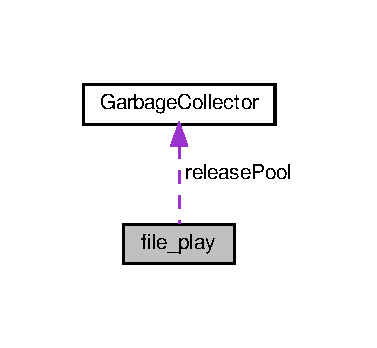
\includegraphics[width=181pt]{classfile__play__coll__graph}
\end{center}
\end{figure}
\subsection*{Classes}
\begin{DoxyCompactItemize}
\item 
struct \hyperlink{structfile__play_1_1playfile__param__t}{playfile\+\_\+param\+\_\+t}
\end{DoxyCompactItemize}
\subsection*{Public Member Functions}
\begin{DoxyCompactItemize}
\item 
\mbox{\Hypertarget{classfile__play_a645ba3e1de2ac795764c06c70a9017c3}\label{classfile__play_a645ba3e1de2ac795764c06c70a9017c3}} 
void {\bfseries rtmha\+\_\+play} (int num\+\_\+sample, float $\ast$out, int channel)
\item 
\mbox{\Hypertarget{classfile__play_a73ab11b570cd0dfb27afd66a1c6d325d}\label{classfile__play_a73ab11b570cd0dfb27afd66a1c6d325d}} 
void {\bfseries set\+\_\+params} (const char $\ast$, int, int, int)
\end{DoxyCompactItemize}
\subsection*{Public Attributes}
\begin{DoxyCompactItemize}
\item 
\mbox{\Hypertarget{classfile__play_aaddaacea18653399886df0fd5c8a4a8b}\label{classfile__play_aaddaacea18653399886df0fd5c8a4a8b}} 
std\+::string {\bfseries root\+Path}
\item 
\mbox{\Hypertarget{classfile__play_a31085df5c45da6b08e325b19180d21e9}\label{classfile__play_a31085df5c45da6b08e325b19180d21e9}} 
std\+::shared\+\_\+ptr$<$ \hyperlink{structfile__play_1_1playfile__param__t}{playfile\+\_\+param\+\_\+t} $>$ {\bfseries current\+Param}
\item 
\mbox{\Hypertarget{classfile__play_a08556103bb7257021f1426faddc6f7fb}\label{classfile__play_a08556103bb7257021f1426faddc6f7fb}} 
\hyperlink{classGarbageCollector}{Garbage\+Collector} {\bfseries release\+Pool}
\end{DoxyCompactItemize}


\subsection{Detailed Description}


Definition at line 7 of file playfile.\+h.



The documentation for this class was generated from the following files\+:\begin{DoxyCompactItemize}
\item 
playfile.\+h\item 
playfile.\+cpp\end{DoxyCompactItemize}

\hypertarget{classfile__record}{}\section{file\+\_\+record Class Reference}
\label{classfile__record}\index{file\+\_\+record@{file\+\_\+record}}


Collaboration diagram for file\+\_\+record\+:\nopagebreak
\begin{figure}[H]
\begin{center}
\leavevmode
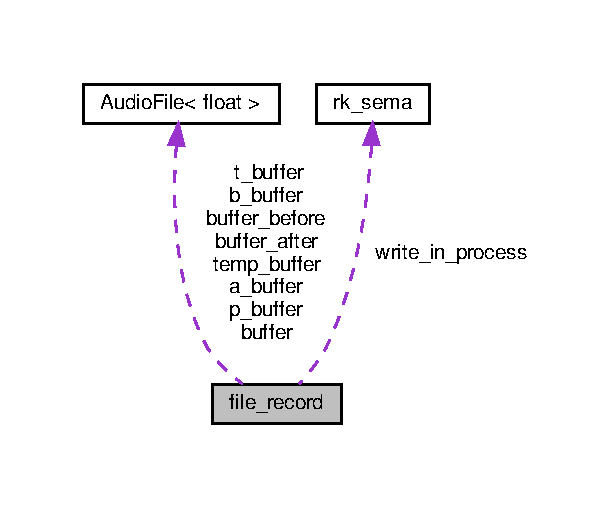
\includegraphics[width=294pt]{classfile__record__coll__graph}
\end{center}
\end{figure}
\subsection*{Public Member Functions}
\begin{DoxyCompactItemize}
\item 
\mbox{\Hypertarget{classfile__record_aa39004a4aed32436d80b694597b37c47}\label{classfile__record_aa39004a4aed32436d80b694597b37c47}} 
{\bfseries file\+\_\+record} (int freq=48000, std\+::string file\+\_\+=\char`\"{}sample.\+wav\char`\"{}, float seconds=5)
\item 
\mbox{\Hypertarget{classfile__record_a8e7f499ae81461bd5a48648ad6aa19c8}\label{classfile__record_a8e7f499ae81461bd5a48648ad6aa19c8}} 
void {\bfseries rtmha\+\_\+record} (int num\+\_\+sample, float $\ast$in, int channel)
\item 
\mbox{\Hypertarget{classfile__record_a9ce4bb8fc603474a050f5c64d423b3f6}\label{classfile__record_a9ce4bb8fc603474a050f5c64d423b3f6}} 
void {\bfseries record\+\_\+before} (int num\+\_\+sample, float $\ast$in, int channel)
\item 
\mbox{\Hypertarget{classfile__record_acf229d7cbf19fd08b62e90ef33ff26c7}\label{classfile__record_acf229d7cbf19fd08b62e90ef33ff26c7}} 
void {\bfseries record\+\_\+after} (int num\+\_\+sample, float $\ast$in, int channel)
\item 
\mbox{\Hypertarget{classfile__record_a39b6f31da58c085a85793f5e77de94bc}\label{classfile__record_a39b6f31da58c085a85793f5e77de94bc}} 
void {\bfseries set\+\_\+params} (int start\+\_\+, int stop\+\_\+, float seconds, const char $\ast$file\+\_\+)
\item 
\mbox{\Hypertarget{classfile__record_ae3d45523d96b17b1b7611daaa493023d}\label{classfile__record_ae3d45523d96b17b1b7611daaa493023d}} 
void {\bfseries get\+\_\+params} (float \&seconds)
\item 
\mbox{\Hypertarget{classfile__record_aab9676316dbd7e767eef34e50d0fe247}\label{classfile__record_aab9676316dbd7e767eef34e50d0fe247}} 
void {\bfseries write\+\_\+to\+\_\+file} ()
\end{DoxyCompactItemize}
\subsection*{Public Attributes}
\begin{DoxyCompactItemize}
\item 
\mbox{\Hypertarget{classfile__record_a2cde61cd39d07b72df01aed74b55a465}\label{classfile__record_a2cde61cd39d07b72df01aed74b55a465}} 
\hyperlink{classAudioFile}{Audio\+File}$<$ float $>$\+::Audio\+Buffer {\bfseries buffer}
\item 
\mbox{\Hypertarget{classfile__record_a29a72f46b29d090b0917f677c5066850}\label{classfile__record_a29a72f46b29d090b0917f677c5066850}} 
\hyperlink{classAudioFile}{Audio\+File}$<$ float $>$\+::Audio\+Buffer {\bfseries temp\+\_\+buffer}
\item 
\mbox{\Hypertarget{classfile__record_a7b2c33679842d309deec6be9684401ee}\label{classfile__record_a7b2c33679842d309deec6be9684401ee}} 
\hyperlink{classAudioFile}{Audio\+File}$<$ float $>$\+::Audio\+Buffer {\bfseries buffer\+\_\+before}
\item 
\mbox{\Hypertarget{classfile__record_a309e591dc171dd5c2f99d6307f7f616c}\label{classfile__record_a309e591dc171dd5c2f99d6307f7f616c}} 
\hyperlink{classAudioFile}{Audio\+File}$<$ float $>$\+::Audio\+Buffer {\bfseries buffer\+\_\+after}
\item 
\mbox{\Hypertarget{classfile__record_a161c3ed15c9b01dbfc552234e63479f4}\label{classfile__record_a161c3ed15c9b01dbfc552234e63479f4}} 
std\+::string {\bfseries root\+Path}
\item 
\mbox{\Hypertarget{classfile__record_acde5edfb344edae7f3f8cf26e363f737}\label{classfile__record_acde5edfb344edae7f3f8cf26e363f737}} 
std\+::string {\bfseries file}
\item 
\mbox{\Hypertarget{classfile__record_ab33ddeca248a16e22312368ad34b2b36}\label{classfile__record_ab33ddeca248a16e22312368ad34b2b36}} 
std\+::atomic$<$ bool $>$ {\bfseries write}
\item 
\mbox{\Hypertarget{classfile__record_a2b6625e3c8db0e24a99cfd2f6c8168cb}\label{classfile__record_a2b6625e3c8db0e24a99cfd2f6c8168cb}} 
\hyperlink{classAudioFile}{Audio\+File}$<$ float $>$\+::Audio\+Buffer $\ast$ {\bfseries p\+\_\+buffer} =0
\item 
\mbox{\Hypertarget{classfile__record_aedccd6a5df58fc9479cd3dbb46e7d151}\label{classfile__record_aedccd6a5df58fc9479cd3dbb46e7d151}} 
\hyperlink{classAudioFile}{Audio\+File}$<$ float $>$\+::Audio\+Buffer $\ast$ {\bfseries t\+\_\+buffer} =0
\item 
\mbox{\Hypertarget{classfile__record_a3e3e09455d86f2efae75b78889db59dd}\label{classfile__record_a3e3e09455d86f2efae75b78889db59dd}} 
\hyperlink{classAudioFile}{Audio\+File}$<$ float $>$\+::Audio\+Buffer $\ast$ {\bfseries b\+\_\+buffer} =\&buffer\+\_\+before
\item 
\mbox{\Hypertarget{classfile__record_a5f89cc7ee12a6361417104e80026a7c6}\label{classfile__record_a5f89cc7ee12a6361417104e80026a7c6}} 
\hyperlink{classAudioFile}{Audio\+File}$<$ float $>$\+::Audio\+Buffer $\ast$ {\bfseries a\+\_\+buffer} =\&buffer\+\_\+after
\item 
\mbox{\Hypertarget{classfile__record_a6253c481183e28aaa0efc7ddd9909828}\label{classfile__record_a6253c481183e28aaa0efc7ddd9909828}} 
int {\bfseries reset}
\item 
\mbox{\Hypertarget{classfile__record_af275a85249908eb6d7d5cbc6889d953a}\label{classfile__record_af275a85249908eb6d7d5cbc6889d953a}} 
int {\bfseries start} =0
\item 
\mbox{\Hypertarget{classfile__record_a90ea367c9a6fcd5841401e38abcd23ec}\label{classfile__record_a90ea367c9a6fcd5841401e38abcd23ec}} 
int {\bfseries stop} =0
\item 
\mbox{\Hypertarget{classfile__record_a3d6e170b7e801452adefb10d75b79878}\label{classfile__record_a3d6e170b7e801452adefb10d75b79878}} 
int {\bfseries start\+\_\+before}
\item 
\mbox{\Hypertarget{classfile__record_a62463eef4f1c081e89522a9848101080}\label{classfile__record_a62463eef4f1c081e89522a9848101080}} 
int {\bfseries start\+\_\+after} =0
\item 
\mbox{\Hypertarget{classfile__record_a88d105ebf3345ee063aa68fe6e6703c4}\label{classfile__record_a88d105ebf3345ee063aa68fe6e6703c4}} 
int {\bfseries stop\+\_\+before} =0
\item 
\mbox{\Hypertarget{classfile__record_a28ac14db371daa3b81300b2f58c34e11}\label{classfile__record_a28ac14db371daa3b81300b2f58c34e11}} 
int {\bfseries stop\+\_\+after}
\item 
\mbox{\Hypertarget{classfile__record_a2f82c2439243c3b026dfd57747ba1862}\label{classfile__record_a2f82c2439243c3b026dfd57747ba1862}} 
int {\bfseries record}
\item 
\mbox{\Hypertarget{classfile__record_a92f31f13d552154a6687f42bbf563d09}\label{classfile__record_a92f31f13d552154a6687f42bbf563d09}} 
int {\bfseries repeat}
\item 
\mbox{\Hypertarget{classfile__record_aaec3da6ffc1e1bcba2177910a291f428}\label{classfile__record_aaec3da6ffc1e1bcba2177910a291f428}} 
std\+::string {\bfseries file\+\_\+path}
\item 
\mbox{\Hypertarget{classfile__record_af78d806a48050161e6fede4c32f51c12}\label{classfile__record_af78d806a48050161e6fede4c32f51c12}} 
int {\bfseries current\+\_\+position\+\_\+l}
\item 
\mbox{\Hypertarget{classfile__record_a091fbe12bf5e70987141666fd5650f0e}\label{classfile__record_a091fbe12bf5e70987141666fd5650f0e}} 
int {\bfseries current\+\_\+position\+\_\+r}
\item 
\mbox{\Hypertarget{classfile__record_a7126513bf737743f045adecaa285ee28}\label{classfile__record_a7126513bf737743f045adecaa285ee28}} 
int {\bfseries current\+\_\+before\+\_\+l}
\item 
\mbox{\Hypertarget{classfile__record_afc198a5acaaffd0ddebc2dae33b79581}\label{classfile__record_afc198a5acaaffd0ddebc2dae33b79581}} 
int {\bfseries current\+\_\+before\+\_\+r}
\item 
\mbox{\Hypertarget{classfile__record_ac87f62e436c4c3861b57656f5fcd05c2}\label{classfile__record_ac87f62e436c4c3861b57656f5fcd05c2}} 
int {\bfseries current\+\_\+after\+\_\+l}
\item 
\mbox{\Hypertarget{classfile__record_a9e5ce706de2d3e8da83d5322dfaaa8c6}\label{classfile__record_a9e5ce706de2d3e8da83d5322dfaaa8c6}} 
int {\bfseries current\+\_\+after\+\_\+r}
\item 
\mbox{\Hypertarget{classfile__record_a8bfcd1e88fa57d9a1adc094d76ec020d}\label{classfile__record_a8bfcd1e88fa57d9a1adc094d76ec020d}} 
int {\bfseries sampling\+\_\+freq}
\item 
\mbox{\Hypertarget{classfile__record_aaf2677460cd4a4a46f1cec592278ec58}\label{classfile__record_aaf2677460cd4a4a46f1cec592278ec58}} 
int {\bfseries num\+Samples}
\item 
\mbox{\Hypertarget{classfile__record_af1ebb968ea657ee1c719a73351d65e4c}\label{classfile__record_af1ebb968ea657ee1c719a73351d65e4c}} 
int {\bfseries num\+Samples\+\_\+before}
\item 
\mbox{\Hypertarget{classfile__record_a8375d9b752bf5280ae48779419b0598a}\label{classfile__record_a8375d9b752bf5280ae48779419b0598a}} 
int {\bfseries num\+Samples\+\_\+after}
\item 
\mbox{\Hypertarget{classfile__record_a80df083a8c4d4f98cea28aeab6f4095e}\label{classfile__record_a80df083a8c4d4f98cea28aeab6f4095e}} 
int {\bfseries finish}
\item 
\mbox{\Hypertarget{classfile__record_a5f1f39d33ec84d708af4c4db016eece4}\label{classfile__record_a5f1f39d33ec84d708af4c4db016eece4}} 
int {\bfseries mono}
\item 
\mbox{\Hypertarget{classfile__record_a0bdcb0ee5740cb1cad3e85ec72d945ef}\label{classfile__record_a0bdcb0ee5740cb1cad3e85ec72d945ef}} 
int {\bfseries t}
\item 
\mbox{\Hypertarget{classfile__record_a6f56fb00f4c4e0cd497168685c1e7064}\label{classfile__record_a6f56fb00f4c4e0cd497168685c1e7064}} 
\hyperlink{structrk__sema}{rk\+\_\+sema} $\ast$ {\bfseries write\+\_\+in\+\_\+process}
\item 
\mbox{\Hypertarget{classfile__record_ab8e447e9e889f3d47f946c2a83928cfa}\label{classfile__record_ab8e447e9e889f3d47f946c2a83928cfa}} 
std\+::thread $\ast$ {\bfseries record\+\_\+thread}
\end{DoxyCompactItemize}


\subsection{Detailed Description}


Definition at line 18 of file file\+\_\+record.\+h.



The documentation for this class was generated from the following files\+:\begin{DoxyCompactItemize}
\item 
file\+\_\+record.\+h\item 
file\+\_\+record.\+cpp\end{DoxyCompactItemize}

\hypertarget{classfilter}{}\section{filter Class Reference}
\label{classfilter}\index{filter@{filter}}


Filter Class.  




{\ttfamily \#include $<$filter.\+hpp$>$}



Inheritance diagram for filter\+:\nopagebreak
\begin{figure}[H]
\begin{center}
\leavevmode
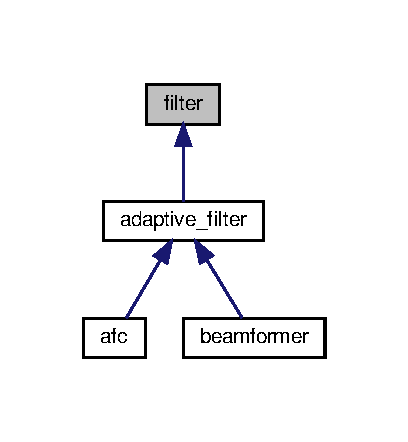
\includegraphics[width=196pt]{classfilter__inherit__graph}
\end{center}
\end{figure}
\subsection*{Public Member Functions}
\begin{DoxyCompactItemize}
\item 
\hyperlink{classfilter_a257d61c89ec8558363f6015fdb9016d7}{filter} (float $\ast$taps, size\+\_\+t tap\+\_\+size, \hyperlink{classcircular__buffer}{circular\+\_\+buffer} $\ast$cir\+\_\+buf, size\+\_\+t max\+\_\+buf\+\_\+size)
\begin{DoxyCompactList}\small\item\em Filter constructor. \end{DoxyCompactList}\item 
\mbox{\Hypertarget{classfilter_a73337fb0e69db82e7c5025e0297ebac5}\label{classfilter_a73337fb0e69db82e7c5025e0297ebac5}} 
\hyperlink{classfilter_a73337fb0e69db82e7c5025e0297ebac5}{$\sim$filter} ()
\begin{DoxyCompactList}\small\item\em Filter destructor. \end{DoxyCompactList}\item 
int \hyperlink{classfilter_a2110dd72f12765f0da1c8e3cb4043a67}{set\+\_\+taps} (const float $\ast$taps, size\+\_\+t buf\+\_\+size)
\begin{DoxyCompactList}\small\item\em Setting the filter taps. \end{DoxyCompactList}\item 
int \hyperlink{classfilter_a9ed7fc2a499abfa2aaffc5477e00fb54}{get\+\_\+taps} (float $\ast$taps, size\+\_\+t buf\+\_\+size)
\begin{DoxyCompactList}\small\item\em Getting the filter taps. \end{DoxyCompactList}\item 
void \hyperlink{classfilter_a983d5bb1cda993859f2a31926d2a5988}{cirfir} (float $\ast$data\+\_\+in, float $\ast$data\+\_\+out, size\+\_\+t num\+\_\+samp)
\begin{DoxyCompactList}\small\item\em Getting the output of this F\+IR filter by performing frame-\/based convolution. \end{DoxyCompactList}\item 
size\+\_\+t \hyperlink{classfilter_a1fe57acd364208770931817c847b725a}{get\+\_\+size} ()
\begin{DoxyCompactList}\small\item\em Getting the number of taps of this F\+IR filter. \end{DoxyCompactList}\item 
void \hyperlink{classfilter_a7fba63872346c69a8e48ca634aa195b3}{cirfir} (float $\ast$data\+\_\+out, size\+\_\+t num\+\_\+samp)
\begin{DoxyCompactList}\small\item\em Frame-\/based convolution for F\+IR filtering. \end{DoxyCompactList}\end{DoxyCompactItemize}


\subsection{Detailed Description}
Filter Class. 

This filter class implements the F\+IR filter 

Definition at line 39 of file filter.\+hpp.



\subsection{Constructor \& Destructor Documentation}
\mbox{\Hypertarget{classfilter_a257d61c89ec8558363f6015fdb9016d7}\label{classfilter_a257d61c89ec8558363f6015fdb9016d7}} 
\index{filter@{filter}!filter@{filter}}
\index{filter@{filter}!filter@{filter}}
\subsubsection{\texorpdfstring{filter()}{filter()}}
{\footnotesize\ttfamily filter\+::filter (\begin{DoxyParamCaption}\item[{float $\ast$}]{taps,  }\item[{size\+\_\+t}]{tap\+\_\+size,  }\item[{\hyperlink{classcircular__buffer}{circular\+\_\+buffer} $\ast$}]{cir\+\_\+buf,  }\item[{size\+\_\+t}]{max\+\_\+buf\+\_\+size }\end{DoxyParamCaption})\hspace{0.3cm}{\ttfamily [explicit]}}



Filter constructor. 


\begin{DoxyParams}[1]{Parameters}
\mbox{\tt in}  & {\em taps} & The filter taps for this F\+IR filter \\
\hline
\mbox{\tt in}  & {\em tap\+\_\+size} & The number of taps of this F\+IR filter \\
\hline
\mbox{\tt in}  & {\em cir\+\_\+buf} & The circular buffer for this F\+IR filter to perform frame-\/based convolution \\
\hline
\mbox{\tt in}  & {\em max\+\_\+buf\+\_\+size} & The maximum size of circular buffer you need to specify if there is no circular buffer given in cir\+\_\+buf \\
\hline
\end{DoxyParams}


Definition at line 31 of file filter.\+cpp.



\subsection{Member Function Documentation}
\mbox{\Hypertarget{classfilter_a983d5bb1cda993859f2a31926d2a5988}\label{classfilter_a983d5bb1cda993859f2a31926d2a5988}} 
\index{filter@{filter}!cirfir@{cirfir}}
\index{cirfir@{cirfir}!filter@{filter}}
\subsubsection{\texorpdfstring{cirfir()}{cirfir()}\hspace{0.1cm}{\footnotesize\ttfamily [1/2]}}
{\footnotesize\ttfamily void filter\+::cirfir (\begin{DoxyParamCaption}\item[{float $\ast$}]{data\+\_\+in,  }\item[{float $\ast$}]{data\+\_\+out,  }\item[{size\+\_\+t}]{num\+\_\+samp }\end{DoxyParamCaption})}



Getting the output of this F\+IR filter by performing frame-\/based convolution. 


\begin{DoxyParams}[1]{Parameters}
\mbox{\tt in}  & {\em data\+\_\+in} & The input signal \\
\hline
\mbox{\tt out}  & {\em data\+\_\+out} & The output signal \\
\hline
 & {\em num\+\_\+samp} & The size of input and output signal (data\+\_\+in and data\+\_\+out should have the same size) \\
\hline
\end{DoxyParams}


Definition at line 96 of file filter.\+cpp.

\mbox{\Hypertarget{classfilter_a7fba63872346c69a8e48ca634aa195b3}\label{classfilter_a7fba63872346c69a8e48ca634aa195b3}} 
\index{filter@{filter}!cirfir@{cirfir}}
\index{cirfir@{cirfir}!filter@{filter}}
\subsubsection{\texorpdfstring{cirfir()}{cirfir()}\hspace{0.1cm}{\footnotesize\ttfamily [2/2]}}
{\footnotesize\ttfamily void filter\+::cirfir (\begin{DoxyParamCaption}\item[{float $\ast$}]{data\+\_\+out,  }\item[{size\+\_\+t}]{num\+\_\+samp }\end{DoxyParamCaption})}



Frame-\/based convolution for F\+IR filtering. 


\begin{DoxyParams}[1]{Parameters}
\mbox{\tt out}  & {\em data\+\_\+out} & The output signal \\
\hline
\mbox{\tt in}  & {\em num\+\_\+samp} & The size of input and output signal \\
\hline
\end{DoxyParams}


Definition at line 107 of file filter.\+cpp.

\mbox{\Hypertarget{classfilter_a1fe57acd364208770931817c847b725a}\label{classfilter_a1fe57acd364208770931817c847b725a}} 
\index{filter@{filter}!get\+\_\+size@{get\+\_\+size}}
\index{get\+\_\+size@{get\+\_\+size}!filter@{filter}}
\subsubsection{\texorpdfstring{get\+\_\+size()}{get\_size()}}
{\footnotesize\ttfamily size\+\_\+t filter\+::get\+\_\+size (\begin{DoxyParamCaption}{ }\end{DoxyParamCaption})}



Getting the number of taps of this F\+IR filter. 

\begin{DoxyReturn}{Returns}
The number of taps of this F\+IR filter 
\end{DoxyReturn}


Definition at line 102 of file filter.\+cpp.

\mbox{\Hypertarget{classfilter_a9ed7fc2a499abfa2aaffc5477e00fb54}\label{classfilter_a9ed7fc2a499abfa2aaffc5477e00fb54}} 
\index{filter@{filter}!get\+\_\+taps@{get\+\_\+taps}}
\index{get\+\_\+taps@{get\+\_\+taps}!filter@{filter}}
\subsubsection{\texorpdfstring{get\+\_\+taps()}{get\_taps()}}
{\footnotesize\ttfamily int filter\+::get\+\_\+taps (\begin{DoxyParamCaption}\item[{float $\ast$}]{taps,  }\item[{size\+\_\+t}]{buf\+\_\+size }\end{DoxyParamCaption})}



Getting the filter taps. 


\begin{DoxyParams}[1]{Parameters}
\mbox{\tt out}  & {\em taps} & The filter taps (1-\/D array) \\
\hline
\mbox{\tt in}  & {\em buf\+\_\+size} & The size of the filter taps (this should be the same as tap\+\_\+size passed in constructor) \\
\hline
\end{DoxyParams}
\begin{DoxyReturn}{Returns}
A flag indicating the success of getting the filter taps 
\end{DoxyReturn}


Definition at line 84 of file filter.\+cpp.

\mbox{\Hypertarget{classfilter_a2110dd72f12765f0da1c8e3cb4043a67}\label{classfilter_a2110dd72f12765f0da1c8e3cb4043a67}} 
\index{filter@{filter}!set\+\_\+taps@{set\+\_\+taps}}
\index{set\+\_\+taps@{set\+\_\+taps}!filter@{filter}}
\subsubsection{\texorpdfstring{set\+\_\+taps()}{set\_taps()}}
{\footnotesize\ttfamily int filter\+::set\+\_\+taps (\begin{DoxyParamCaption}\item[{const float $\ast$}]{taps,  }\item[{size\+\_\+t}]{buf\+\_\+size }\end{DoxyParamCaption})}



Setting the filter taps. 


\begin{DoxyParams}[1]{Parameters}
\mbox{\tt in}  & {\em taps} & The filter taps (an 1-\/D array) \\
\hline
\mbox{\tt in}  & {\em buf\+\_\+size} & The size of the filter taps (this should be the same as tap\+\_\+size passed in constructor) \\
\hline
\end{DoxyParams}
\begin{DoxyReturn}{Returns}
A flag indicating the success of setting the filter taps 
\end{DoxyReturn}


Definition at line 68 of file filter.\+cpp.



The documentation for this class was generated from the following files\+:\begin{DoxyCompactItemize}
\item 
\hyperlink{filter_8hpp}{filter.\+hpp}\item 
\hyperlink{filter_8cpp}{filter.\+cpp}\end{DoxyCompactItemize}

\hypertarget{classfir__formii}{}\section{fir\+\_\+formii Class Reference}
\label{classfir__formii}\index{fir\+\_\+formii@{fir\+\_\+formii}}


Filter Class.  




{\ttfamily \#include $<$fir\+\_\+formii.\+h$>$}

\subsection*{Public Member Functions}
\begin{DoxyCompactItemize}
\item 
\hyperlink{classfir__formii_a1b2824e6a0f6f9065e86d43676432b37}{fir\+\_\+formii} (float $\ast$taps, size\+\_\+t tap\+\_\+size)
\begin{DoxyCompactList}\small\item\em Filter constructor. \end{DoxyCompactList}\item 
\mbox{\Hypertarget{classfir__formii_ac9b5d5e8b0a2b2cad69a6b7935e87f19}\label{classfir__formii_ac9b5d5e8b0a2b2cad69a6b7935e87f19}} 
\hyperlink{classfir__formii_ac9b5d5e8b0a2b2cad69a6b7935e87f19}{$\sim$fir\+\_\+formii} ()
\begin{DoxyCompactList}\small\item\em Filter destructor. \end{DoxyCompactList}\item 
void \hyperlink{classfir__formii_a35f410bda8c31d821ec438707b0bca10}{set\+\_\+taps} (const float $\ast$taps, size\+\_\+t tap\+\_\+size)
\begin{DoxyCompactList}\small\item\em Setting the filter taps. \end{DoxyCompactList}\item 
void \hyperlink{classfir__formii_a11e18bf6b5c6ffcb8979bb0ecf7436e1}{get\+\_\+taps} (float $\ast$taps, size\+\_\+t \&tap\+\_\+size)
\begin{DoxyCompactList}\small\item\em Getting the filter taps. \end{DoxyCompactList}\item 
void \hyperlink{classfir__formii_ac9b081bf01b911fbbbd354e0c3b61e94}{process} (const float $\ast$data\+\_\+in, float $\ast$data\+\_\+out, size\+\_\+t num\+\_\+samp)
\begin{DoxyCompactList}\small\item\em Getting the output of this F\+IR filter by performing frame-\/based convolution. \end{DoxyCompactList}\item 
size\+\_\+t \hyperlink{classfir__formii_af2225fdc109c072f68840975b6e269fd}{get\+\_\+size} ()
\begin{DoxyCompactList}\small\item\em Getting the number of taps of this F\+IR filter. \end{DoxyCompactList}\end{DoxyCompactItemize}


\subsection{Detailed Description}
Filter Class. 

This filter class implements the F\+IR filter 

Definition at line 41 of file fir\+\_\+formii.\+h.



\subsection{Constructor \& Destructor Documentation}
\mbox{\Hypertarget{classfir__formii_a1b2824e6a0f6f9065e86d43676432b37}\label{classfir__formii_a1b2824e6a0f6f9065e86d43676432b37}} 
\index{fir\+\_\+formii@{fir\+\_\+formii}!fir\+\_\+formii@{fir\+\_\+formii}}
\index{fir\+\_\+formii@{fir\+\_\+formii}!fir\+\_\+formii@{fir\+\_\+formii}}
\subsubsection{\texorpdfstring{fir\+\_\+formii()}{fir\_formii()}}
{\footnotesize\ttfamily fir\+\_\+formii\+::fir\+\_\+formii (\begin{DoxyParamCaption}\item[{float $\ast$}]{taps,  }\item[{size\+\_\+t}]{tap\+\_\+size }\end{DoxyParamCaption})\hspace{0.3cm}{\ttfamily [explicit]}}



Filter constructor. 


\begin{DoxyParams}[1]{Parameters}
\mbox{\tt in}  & {\em taps} & The filter taps for this F\+IR filter \\
\hline
\mbox{\tt in}  & {\em tap\+\_\+size} & The number of taps of this F\+IR filter \\
\hline
\mbox{\tt in}  & {\em cir\+\_\+buf} & The circular buffer for this F\+IR filter to perform frame-\/based convolution \\
\hline
\mbox{\tt in}  & {\em max\+\_\+buf\+\_\+size} & The maximum size of circular buffer you need to specify if there is no circular buffer given in cir\+\_\+buf \\
\hline
\end{DoxyParams}


Definition at line 29 of file fir\+\_\+formii.\+cpp.



\subsection{Member Function Documentation}
\mbox{\Hypertarget{classfir__formii_af2225fdc109c072f68840975b6e269fd}\label{classfir__formii_af2225fdc109c072f68840975b6e269fd}} 
\index{fir\+\_\+formii@{fir\+\_\+formii}!get\+\_\+size@{get\+\_\+size}}
\index{get\+\_\+size@{get\+\_\+size}!fir\+\_\+formii@{fir\+\_\+formii}}
\subsubsection{\texorpdfstring{get\+\_\+size()}{get\_size()}}
{\footnotesize\ttfamily size\+\_\+t fir\+\_\+formii\+::get\+\_\+size (\begin{DoxyParamCaption}{ }\end{DoxyParamCaption})}



Getting the number of taps of this F\+IR filter. 

\begin{DoxyReturn}{Returns}
The number of taps of this F\+IR filter 
\end{DoxyReturn}


Definition at line 97 of file fir\+\_\+formii.\+cpp.

\mbox{\Hypertarget{classfir__formii_a11e18bf6b5c6ffcb8979bb0ecf7436e1}\label{classfir__formii_a11e18bf6b5c6ffcb8979bb0ecf7436e1}} 
\index{fir\+\_\+formii@{fir\+\_\+formii}!get\+\_\+taps@{get\+\_\+taps}}
\index{get\+\_\+taps@{get\+\_\+taps}!fir\+\_\+formii@{fir\+\_\+formii}}
\subsubsection{\texorpdfstring{get\+\_\+taps()}{get\_taps()}}
{\footnotesize\ttfamily void fir\+\_\+formii\+::get\+\_\+taps (\begin{DoxyParamCaption}\item[{float $\ast$}]{taps,  }\item[{size\+\_\+t \&}]{tap\+\_\+size }\end{DoxyParamCaption})}



Getting the filter taps. 


\begin{DoxyParams}[1]{Parameters}
\mbox{\tt out}  & {\em taps} & The filter taps (1-\/D array) \\
\hline
\mbox{\tt in}  & {\em buf\+\_\+size} & The size of the filter taps (this should be the same as tap\+\_\+size passed in constructor) \\
\hline
\end{DoxyParams}
\begin{DoxyReturn}{Returns}
A flag indicating the success of getting the filter taps 
\end{DoxyReturn}


Definition at line 65 of file fir\+\_\+formii.\+cpp.

\mbox{\Hypertarget{classfir__formii_ac9b081bf01b911fbbbd354e0c3b61e94}\label{classfir__formii_ac9b081bf01b911fbbbd354e0c3b61e94}} 
\index{fir\+\_\+formii@{fir\+\_\+formii}!process@{process}}
\index{process@{process}!fir\+\_\+formii@{fir\+\_\+formii}}
\subsubsection{\texorpdfstring{process()}{process()}}
{\footnotesize\ttfamily void fir\+\_\+formii\+::process (\begin{DoxyParamCaption}\item[{const float $\ast$}]{data\+\_\+in,  }\item[{float $\ast$}]{data\+\_\+out,  }\item[{size\+\_\+t}]{num\+\_\+samp }\end{DoxyParamCaption})}



Getting the output of this F\+IR filter by performing frame-\/based convolution. 


\begin{DoxyParams}[1]{Parameters}
\mbox{\tt in}  & {\em data\+\_\+in} & The input signal \\
\hline
\mbox{\tt out}  & {\em data\+\_\+out} & The output signal \\
\hline
 & {\em num\+\_\+samp} & The size of input and output signal (data\+\_\+in and data\+\_\+out should have the same size) \\
\hline
\end{DoxyParams}


Definition at line 73 of file fir\+\_\+formii.\+cpp.

\mbox{\Hypertarget{classfir__formii_a35f410bda8c31d821ec438707b0bca10}\label{classfir__formii_a35f410bda8c31d821ec438707b0bca10}} 
\index{fir\+\_\+formii@{fir\+\_\+formii}!set\+\_\+taps@{set\+\_\+taps}}
\index{set\+\_\+taps@{set\+\_\+taps}!fir\+\_\+formii@{fir\+\_\+formii}}
\subsubsection{\texorpdfstring{set\+\_\+taps()}{set\_taps()}}
{\footnotesize\ttfamily void fir\+\_\+formii\+::set\+\_\+taps (\begin{DoxyParamCaption}\item[{const float $\ast$}]{taps,  }\item[{size\+\_\+t}]{tap\+\_\+size }\end{DoxyParamCaption})}



Setting the filter taps. 


\begin{DoxyParams}[1]{Parameters}
\mbox{\tt in}  & {\em taps} & The filter taps (an 1-\/D array) \\
\hline
\mbox{\tt in}  & {\em buf\+\_\+size} & The size of the filter taps (this should be the same as tap\+\_\+size passed in constructor) \\
\hline
\end{DoxyParams}
\begin{DoxyReturn}{Returns}
A flag indicating the success of setting the filter taps 
\end{DoxyReturn}


Definition at line 49 of file fir\+\_\+formii.\+cpp.



The documentation for this class was generated from the following files\+:\begin{DoxyCompactItemize}
\item 
\hyperlink{fir__formii_8h}{fir\+\_\+formii.\+h}\item 
\hyperlink{fir__formii_8cpp}{fir\+\_\+formii.\+cpp}\end{DoxyCompactItemize}

\hypertarget{classfreping}{}\section{freping Class Reference}
\label{classfreping}\index{freping@{freping}}


Freping Class.  




{\ttfamily \#include $<$freping.\+hpp$>$}

\subsection*{Public Member Functions}
\begin{DoxyCompactItemize}
\item 
\hyperlink{classfreping_a2df9985dad679cb5f796d75367b28b2c}{freping} (int allpass\+\_\+chain\+\_\+len, int frame\+\_\+size, float alpha, float $\ast$window, int freping\+\_\+on\+\_\+off)
\begin{DoxyCompactList}\small\item\em Freping constructor. \end{DoxyCompactList}\item 
\mbox{\Hypertarget{classfreping_a9af0fab164c325edb28cd97a8dcaf74a}\label{classfreping_a9af0fab164c325edb28cd97a8dcaf74a}} 
\hyperlink{classfreping_a9af0fab164c325edb28cd97a8dcaf74a}{$\sim$freping} ()
\begin{DoxyCompactList}\small\item\em Freping destructor. \end{DoxyCompactList}\item 
void \hyperlink{classfreping_a0028d0a70f920dddae2d8fab614de880}{get\+\_\+params} (float \&alpha, int \&freping\+\_\+on\+\_\+off)
\begin{DoxyCompactList}\small\item\em Get the parameter alpha. \end{DoxyCompactList}\item 
void \hyperlink{classfreping_acb0eb9617755641b866e8fc9c84681cd}{set\+\_\+params} (float alpha, int freping\+\_\+on\+\_\+off)
\begin{DoxyCompactList}\small\item\em Set the parameter alpha. \end{DoxyCompactList}\item 
void \hyperlink{classfreping_a610d4b0c36b090709808dac0fe57dc77}{freping\+\_\+proc} (float $\ast$in, float $\ast$out)
\end{DoxyCompactItemize}
\subsection*{Protected Member Functions}
\begin{DoxyCompactItemize}
\item 
void \hyperlink{classfreping_abf4dad3740451d41a9462b1994df09bd}{overlap\+\_\+add} (const float $\ast$in, float $\ast$out)
\item 
void \hyperlink{classfreping_a5ac5fad6ea8f20a8ced37c05b779f077}{allpass\+\_\+chain} (float $\ast$in, float $\ast$out, float alpha\+\_\+, float coeff\+\_\+)
\begin{DoxyCompactList}\small\item\em The all-\/pass chain which has the length of allpass\+\_\+chain\+\_\+len. \end{DoxyCompactList}\item 
void \hyperlink{classfreping_a68ae299fddc13981c0dacc2b7d2bb06f}{windowing} (const float $\ast$in, float $\ast$out)
\end{DoxyCompactItemize}


\subsection{Detailed Description}
Freping Class. 

This freping class provides frequency warping feature in real-\/time. Please refer to the following paper for details. Ching-\/\+Hua Lee, Kuan-\/\+Lin Chen, fred harris, Bhaskar D. Rao, and Harinath Garudadri, \char`\"{}\+On mitigating acoustic feedback in hearing aids with frequency warping by all-\/pass networks,\char`\"{} in Annual Conference of the International Speech Communication Association (Interspeech), 2019. 

Definition at line 44 of file freping.\+hpp.



\subsection{Constructor \& Destructor Documentation}
\mbox{\Hypertarget{classfreping_a2df9985dad679cb5f796d75367b28b2c}\label{classfreping_a2df9985dad679cb5f796d75367b28b2c}} 
\index{freping@{freping}!freping@{freping}}
\index{freping@{freping}!freping@{freping}}
\subsubsection{\texorpdfstring{freping()}{freping()}}
{\footnotesize\ttfamily freping\+::freping (\begin{DoxyParamCaption}\item[{int}]{allpass\+\_\+chain\+\_\+len,  }\item[{int}]{frame\+\_\+size,  }\item[{float}]{alpha,  }\item[{float $\ast$}]{window,  }\item[{int}]{freping\+\_\+on\+\_\+off }\end{DoxyParamCaption})\hspace{0.3cm}{\ttfamily [explicit]}}



Freping constructor. 


\begin{DoxyParams}[1]{Parameters}
\mbox{\tt in}  & {\em allpass\+\_\+chain\+\_\+len} & The length of the all-\/pass chain \\
\hline
\mbox{\tt in}  & {\em frame\+\_\+size} & The frame size of the caller (the real-\/time system) \\
\hline
\mbox{\tt in}  & {\em alpha} & The parameter to control the degree of frequency warping (1.\+0$>$=alpha$>$=-\/1.\+0) \\
\hline
\end{DoxyParams}
As long as this is true we don\textquotesingle{}t need circular buf function 

Definition at line 29 of file freping.\+cpp.



\subsection{Member Function Documentation}
\mbox{\Hypertarget{classfreping_a5ac5fad6ea8f20a8ced37c05b779f077}\label{classfreping_a5ac5fad6ea8f20a8ced37c05b779f077}} 
\index{freping@{freping}!allpass\+\_\+chain@{allpass\+\_\+chain}}
\index{allpass\+\_\+chain@{allpass\+\_\+chain}!freping@{freping}}
\subsubsection{\texorpdfstring{allpass\+\_\+chain()}{allpass\_chain()}}
{\footnotesize\ttfamily void freping\+::allpass\+\_\+chain (\begin{DoxyParamCaption}\item[{float $\ast$}]{in,  }\item[{float $\ast$}]{out,  }\item[{float}]{alpha\+\_\+,  }\item[{float}]{coeff\+\_\+ }\end{DoxyParamCaption})\hspace{0.3cm}{\ttfamily [protected]}}



The all-\/pass chain which has the length of allpass\+\_\+chain\+\_\+len. 


\begin{DoxyParams}[1]{Parameters}
\mbox{\tt in}  & {\em in} & The input frame which has the same size of the output frame (e.\+g., 128 samples) \\
\hline
\mbox{\tt out}  & {\em out} & The output frame (e.\+g., 128 samples) \\
\hline
\mbox{\tt in}  & {\em alpha\+\_\+} & The parameter to control the degree of frequency warping (1.\+0$>$=alpha$>$=-\/1.\+0) \\
\hline
\mbox{\tt in}  & {\em coeff\+\_\+} & a coefficient for the second I\+IR filter in the all-\/pass chain (a function of alpha\+\_\+) \\
\hline
\end{DoxyParams}
the fist stage of the all-\/pass chain

the second stage of the all-\/pass chain

Pointer swaping cost less than copying memory

the remaining stages of the all-\/pass chain

Pointer swaping cost less than copying memory 

Definition at line 78 of file freping.\+cpp.

\mbox{\Hypertarget{classfreping_a610d4b0c36b090709808dac0fe57dc77}\label{classfreping_a610d4b0c36b090709808dac0fe57dc77}} 
\index{freping@{freping}!freping\+\_\+proc@{freping\+\_\+proc}}
\index{freping\+\_\+proc@{freping\+\_\+proc}!freping@{freping}}
\subsubsection{\texorpdfstring{freping\+\_\+proc()}{freping\_proc()}}
{\footnotesize\ttfamily void freping\+::freping\+\_\+proc (\begin{DoxyParamCaption}\item[{float $\ast$}]{in,  }\item[{float $\ast$}]{out }\end{DoxyParamCaption})}

Get the output signal of freping, the output signal is warped according to the alpha parameter 
\begin{DoxyParams}[1]{Parameters}
\mbox{\tt in}  & {\em in} & The input frame \\
\hline
\mbox{\tt out}  & {\em out} & The output frame \\
\hline
\end{DoxyParams}
in\+\_\+buf\+\_\+-\/$>$set(in,frame\+\_\+size\+\_\+); // Do we really need if frame\+\_\+size is already a multiple of all\+\_\+pass\+\_\+len m\+\_\+ = ++run\+\_\+k\+\_\+; /// Why is this useful?

in\+\_\+buf\+\_\+-\/$>$get(x\+\_\+buf\+\_\+,buf\+\_\+len\+\_\+); this-\/$>$overlap\+\_\+framing(x\+\_\+buf\+\_\+,overlapped\+\_\+frame\+\_\+);

Pointer swaping cost less than copying memory 

Definition at line 157 of file freping.\+cpp.

\mbox{\Hypertarget{classfreping_a0028d0a70f920dddae2d8fab614de880}\label{classfreping_a0028d0a70f920dddae2d8fab614de880}} 
\index{freping@{freping}!get\+\_\+params@{get\+\_\+params}}
\index{get\+\_\+params@{get\+\_\+params}!freping@{freping}}
\subsubsection{\texorpdfstring{get\+\_\+params()}{get\_params()}}
{\footnotesize\ttfamily void freping\+::get\+\_\+params (\begin{DoxyParamCaption}\item[{float \&}]{alpha,  }\item[{int \&}]{freping\+\_\+on\+\_\+off }\end{DoxyParamCaption})}



Get the parameter alpha. 


\begin{DoxyParams}[1]{Parameters}
\mbox{\tt out}  & {\em alpha} & The parameter to control the degree of frequency warping (1.\+0$>$=alpha$>$=-\/1.\+0) \\
\hline
\end{DoxyParams}


Definition at line 133 of file freping.\+cpp.

\mbox{\Hypertarget{classfreping_abf4dad3740451d41a9462b1994df09bd}\label{classfreping_abf4dad3740451d41a9462b1994df09bd}} 
\index{freping@{freping}!overlap\+\_\+add@{overlap\+\_\+add}}
\index{overlap\+\_\+add@{overlap\+\_\+add}!freping@{freping}}
\subsubsection{\texorpdfstring{overlap\+\_\+add()}{overlap\_add()}}
{\footnotesize\ttfamily void freping\+::overlap\+\_\+add (\begin{DoxyParamCaption}\item[{const float $\ast$}]{in,  }\item[{float $\ast$}]{out }\end{DoxyParamCaption})\hspace{0.3cm}{\ttfamily [protected]}}

Overlap-\/add method 
\begin{DoxyParams}[1]{Parameters}
\mbox{\tt in}  & {\em in} & The overlapped frame which has the twice size of the output frame (e.\+g., 128 samples) \\
\hline
\mbox{\tt out}  & {\em out} & The recovered frame (e.\+g., 64 samples) \\
\hline
\end{DoxyParams}
This should do the same thing 

Definition at line 119 of file freping.\+cpp.

\mbox{\Hypertarget{classfreping_acb0eb9617755641b866e8fc9c84681cd}\label{classfreping_acb0eb9617755641b866e8fc9c84681cd}} 
\index{freping@{freping}!set\+\_\+params@{set\+\_\+params}}
\index{set\+\_\+params@{set\+\_\+params}!freping@{freping}}
\subsubsection{\texorpdfstring{set\+\_\+params()}{set\_params()}}
{\footnotesize\ttfamily void freping\+::set\+\_\+params (\begin{DoxyParamCaption}\item[{float}]{alpha,  }\item[{int}]{freping\+\_\+on\+\_\+off }\end{DoxyParamCaption})}



Set the parameter alpha. 


\begin{DoxyParams}[1]{Parameters}
\mbox{\tt in}  & {\em alpha} & The parameter to control the degree of frequency warping (1.\+0$>$=alpha$>$=-\/1.\+0) \\
\hline
\end{DoxyParams}


Definition at line 139 of file freping.\+cpp.

\mbox{\Hypertarget{classfreping_a68ae299fddc13981c0dacc2b7d2bb06f}\label{classfreping_a68ae299fddc13981c0dacc2b7d2bb06f}} 
\index{freping@{freping}!windowing@{windowing}}
\index{windowing@{windowing}!freping@{freping}}
\subsubsection{\texorpdfstring{windowing()}{windowing()}}
{\footnotesize\ttfamily void freping\+::windowing (\begin{DoxyParamCaption}\item[{const float $\ast$}]{in,  }\item[{float $\ast$}]{out }\end{DoxyParamCaption})\hspace{0.3cm}{\ttfamily [protected]}}

Applying a window function such as Hamming window to the input frame 
\begin{DoxyParams}[1]{Parameters}
\mbox{\tt in}  & {\em in} & The input frame which has the same size of the output frame (e.\+g., 128 samples) \\
\hline
\mbox{\tt out}  & {\em out} & The output frame (e.\+g., 128 samples) \\
\hline
\end{DoxyParams}


Definition at line 72 of file freping.\+cpp.



The documentation for this class was generated from the following files\+:\begin{DoxyCompactItemize}
\item 
\hyperlink{freping_8hpp}{freping.\+hpp}\item 
\hyperlink{freping_8cpp}{freping.\+cpp}\end{DoxyCompactItemize}

\hypertarget{classGarbageCollector}{}\section{Garbage\+Collector Class Reference}
\label{classGarbageCollector}\index{Garbage\+Collector@{Garbage\+Collector}}
\subsection*{Public Member Functions}
\begin{DoxyCompactItemize}
\item 
\mbox{\Hypertarget{classGarbageCollector_a714258c044ec11c93dcbce058b11b90e}\label{classGarbageCollector_a714258c044ec11c93dcbce058b11b90e}} 
{\footnotesize template$<$typename T $>$ }\\void {\bfseries add} (const std\+::shared\+\_\+ptr$<$ T $>$ \&object)
\item 
\mbox{\Hypertarget{classGarbageCollector_aa33d6dfb5b26b3ac9d455918646af44a}\label{classGarbageCollector_aa33d6dfb5b26b3ac9d455918646af44a}} 
void {\bfseries release} ()
\end{DoxyCompactItemize}
\subsection*{Public Attributes}
\begin{DoxyCompactItemize}
\item 
\mbox{\Hypertarget{classGarbageCollector_adc7048b3a2d2ba24e21b7266dfe4b42e}\label{classGarbageCollector_adc7048b3a2d2ba24e21b7266dfe4b42e}} 
std\+::vector$<$ std\+::shared\+\_\+ptr$<$ void $>$ $>$ {\bfseries pool}
\item 
\mbox{\Hypertarget{classGarbageCollector_a43200fd65ff71d251ec8d0c52776ed6a}\label{classGarbageCollector_a43200fd65ff71d251ec8d0c52776ed6a}} 
std\+::mutex {\bfseries m}
\end{DoxyCompactItemize}


\subsection{Detailed Description}


Definition at line 36 of file Garbage\+Collector.\+hpp.



The documentation for this class was generated from the following file\+:\begin{DoxyCompactItemize}
\item 
Garbage\+Collector.\+hpp\end{DoxyCompactItemize}

\hypertarget{classlibModule}{}\section{lib\+Module Class Reference}
\label{classlibModule}\index{lib\+Module@{lib\+Module}}


A template for library modules.  


\subsection*{Public Member Functions}
\begin{DoxyCompactItemize}
\item 
\mbox{\Hypertarget{classlibModule_aea7a75e970a43e44eaa400427cd8ff12}\label{classlibModule_aea7a75e970a43e44eaa400427cd8ff12}} 
\hyperlink{classlibModule_aea7a75e970a43e44eaa400427cd8ff12}{lib\+Module} (...)
\begin{DoxyCompactList}\small\item\em \hyperlink{classlibModule}{lib\+Module} constructor \end{DoxyCompactList}\item 
\mbox{\Hypertarget{classlibModule_a80881d812a85c51472d78f79209439d0}\label{classlibModule_a80881d812a85c51472d78f79209439d0}} 
\hyperlink{classlibModule_a80881d812a85c51472d78f79209439d0}{$\sim$lib\+Module} ()
\begin{DoxyCompactList}\small\item\em \hyperlink{classlibModule}{lib\+Module} destructor \end{DoxyCompactList}\item 
\mbox{\Hypertarget{classlibModule_ad9facd367f2700af9064c3100e635379}\label{classlibModule_ad9facd367f2700af9064c3100e635379}} 
void \hyperlink{classlibModule_ad9facd367f2700af9064c3100e635379}{set\+\_\+param} (...)
\begin{DoxyCompactList}\small\item\em Setting \hyperlink{classlibModule}{lib\+Module} parameters. \end{DoxyCompactList}\item 
\mbox{\Hypertarget{classlibModule_a29e54e26959d3fb1339b0442afdf6d7e}\label{classlibModule_a29e54e26959d3fb1339b0442afdf6d7e}} 
void \hyperlink{classlibModule_a29e54e26959d3fb1339b0442afdf6d7e}{get\+\_\+param} (...)
\begin{DoxyCompactList}\small\item\em Getting \hyperlink{classlibModule}{lib\+Module} parameters. \end{DoxyCompactList}\item 
\mbox{\Hypertarget{classlibModule_af3049f489a9efea1f630418f11efa8d6}\label{classlibModule_af3049f489a9efea1f630418f11efa8d6}} 
void \hyperlink{classlibModule_af3049f489a9efea1f630418f11efa8d6}{process} (...)
\begin{DoxyCompactList}\small\item\em Real-\/time processing inside \hyperlink{classlibModule}{lib\+Module}. \end{DoxyCompactList}\end{DoxyCompactItemize}


\subsection{Detailed Description}
A template for library modules. 

Definition at line 16 of file example\+\_\+template.\+cpp.



The documentation for this class was generated from the following file\+:\begin{DoxyCompactItemize}
\item 
example\+\_\+template.\+cpp\end{DoxyCompactItemize}

\hypertarget{classnoise__management}{}\section{noise\+\_\+management Class Reference}
\label{classnoise__management}\index{noise\+\_\+management@{noise\+\_\+management}}


Noise Management Class.  




{\ttfamily \#include $<$noise\+\_\+management.\+hpp$>$}

\subsection*{Public Member Functions}
\begin{DoxyCompactItemize}
\item 
\hyperlink{classnoise__management_a2285f3bb163f38f773cf5d6ccbd6022e}{noise\+\_\+management} (int ntype, int stype, float sparam, float fsamp)
\begin{DoxyCompactList}\small\item\em Noise management constructor. \end{DoxyCompactList}\item 
\mbox{\Hypertarget{classnoise__management_a9a0a09f3048e97a98d3278e233096530}\label{classnoise__management_a9a0a09f3048e97a98d3278e233096530}} 
\hyperlink{classnoise__management_a9a0a09f3048e97a98d3278e233096530}{$\sim$noise\+\_\+management} ()
\begin{DoxyCompactList}\small\item\em Noise management destructor. \end{DoxyCompactList}\item 
void \hyperlink{classnoise__management_a50d6db52a6a83aef67e42c4a9f879cc5}{set\+\_\+param} (int ntype, int stype, float sparam)
\begin{DoxyCompactList}\small\item\em Setting all parameters in noise management. \end{DoxyCompactList}\item 
void \hyperlink{classnoise__management_af5fe32222b7fe86d4ec3222e2f60ede7}{get\+\_\+param} (int \&ntype, int \&stype, float \&sparam)
\begin{DoxyCompactList}\small\item\em Getting all parameters in noise management. \end{DoxyCompactList}\item 
void \hyperlink{classnoise__management_aa73425faa4f2434bf26a27c7068bbd1a}{speech\+\_\+enhancement} (float $\ast$data\+\_\+in, size\+\_\+t in\+\_\+len, float $\ast$data\+\_\+out)
\begin{DoxyCompactList}\small\item\em A function to perform speech enhancement. \end{DoxyCompactList}\end{DoxyCompactItemize}


\subsection{Detailed Description}
Noise Management Class. 

Speech enhancement using peak and valley detection, noise estimation and spectral subtraction 

Definition at line 16 of file noise\+\_\+management.\+hpp.



\subsection{Constructor \& Destructor Documentation}
\mbox{\Hypertarget{classnoise__management_a2285f3bb163f38f773cf5d6ccbd6022e}\label{classnoise__management_a2285f3bb163f38f773cf5d6ccbd6022e}} 
\index{noise\+\_\+management@{noise\+\_\+management}!noise\+\_\+management@{noise\+\_\+management}}
\index{noise\+\_\+management@{noise\+\_\+management}!noise\+\_\+management@{noise\+\_\+management}}
\subsubsection{\texorpdfstring{noise\+\_\+management()}{noise\_management()}}
{\footnotesize\ttfamily noise\+\_\+management\+::noise\+\_\+management (\begin{DoxyParamCaption}\item[{int}]{ntype,  }\item[{int}]{stype,  }\item[{float}]{sparam,  }\item[{float}]{fsamp }\end{DoxyParamCaption})\hspace{0.3cm}{\ttfamily [explicit]}}



Noise management constructor. 


\begin{DoxyParams}[1]{Parameters}
\mbox{\tt in}  & {\em ntype} & The type of noise estimation, 1\+: using limits on change (ref\+: Arslan et al.), 2\+: using the weighted averaging of Hirsch and Ehrlicher, 3\+: using M\+C\+RA of Cohen and Berdugo \\
\hline
\mbox{\tt in}  & {\em stype} & The type of spectral subtraction, 0\+: normal, 1\+: oversubtraction \\
\hline
\mbox{\tt in}  & {\em sparam} & A parameter for spectral subtraction \\
\hline
\mbox{\tt in}  & {\em fsamp} & The sampling rate \\
\hline
\end{DoxyParams}


Definition at line 5 of file noise\+\_\+management.\+cpp.



\subsection{Member Function Documentation}
\mbox{\Hypertarget{classnoise__management_af5fe32222b7fe86d4ec3222e2f60ede7}\label{classnoise__management_af5fe32222b7fe86d4ec3222e2f60ede7}} 
\index{noise\+\_\+management@{noise\+\_\+management}!get\+\_\+param@{get\+\_\+param}}
\index{get\+\_\+param@{get\+\_\+param}!noise\+\_\+management@{noise\+\_\+management}}
\subsubsection{\texorpdfstring{get\+\_\+param()}{get\_param()}}
{\footnotesize\ttfamily void noise\+\_\+management\+::get\+\_\+param (\begin{DoxyParamCaption}\item[{int \&}]{ntype,  }\item[{int \&}]{stype,  }\item[{float \&}]{sparam }\end{DoxyParamCaption})}



Getting all parameters in noise management. 


\begin{DoxyParams}[1]{Parameters}
\mbox{\tt in}  & {\em ntype} & See constructor \\
\hline
\mbox{\tt in}  & {\em stype} & See constructor \\
\hline
\mbox{\tt in}  & {\em sparam} & See constructor \\
\hline
\end{DoxyParams}


Definition at line 86 of file noise\+\_\+management.\+cpp.

\mbox{\Hypertarget{classnoise__management_a50d6db52a6a83aef67e42c4a9f879cc5}\label{classnoise__management_a50d6db52a6a83aef67e42c4a9f879cc5}} 
\index{noise\+\_\+management@{noise\+\_\+management}!set\+\_\+param@{set\+\_\+param}}
\index{set\+\_\+param@{set\+\_\+param}!noise\+\_\+management@{noise\+\_\+management}}
\subsubsection{\texorpdfstring{set\+\_\+param()}{set\_param()}}
{\footnotesize\ttfamily void noise\+\_\+management\+::set\+\_\+param (\begin{DoxyParamCaption}\item[{int}]{ntype,  }\item[{int}]{stype,  }\item[{float}]{sparam }\end{DoxyParamCaption})}



Setting all parameters in noise management. 


\begin{DoxyParams}[1]{Parameters}
\mbox{\tt in}  & {\em ntype} & See constructor \\
\hline
\mbox{\tt in}  & {\em stype} & See constructor \\
\hline
\mbox{\tt in}  & {\em sparam} & See constructor \\
\hline
\end{DoxyParams}


Definition at line 77 of file noise\+\_\+management.\+cpp.

\mbox{\Hypertarget{classnoise__management_aa73425faa4f2434bf26a27c7068bbd1a}\label{classnoise__management_aa73425faa4f2434bf26a27c7068bbd1a}} 
\index{noise\+\_\+management@{noise\+\_\+management}!speech\+\_\+enhancement@{speech\+\_\+enhancement}}
\index{speech\+\_\+enhancement@{speech\+\_\+enhancement}!noise\+\_\+management@{noise\+\_\+management}}
\subsubsection{\texorpdfstring{speech\+\_\+enhancement()}{speech\_enhancement()}}
{\footnotesize\ttfamily void noise\+\_\+management\+::speech\+\_\+enhancement (\begin{DoxyParamCaption}\item[{float $\ast$}]{data\+\_\+in,  }\item[{size\+\_\+t}]{in\+\_\+len,  }\item[{float $\ast$}]{data\+\_\+out }\end{DoxyParamCaption})}



A function to perform speech enhancement. 


\begin{DoxyParams}[1]{Parameters}
\mbox{\tt in}  & {\em data\+\_\+in} & The input signal \\
\hline
\mbox{\tt in}  & {\em in\+\_\+len} & Length of the input signal \\
\hline
\mbox{\tt out}  & {\em data\+\_\+out} & The output signal, i.\+e., the enhanced speech signal \\
\hline
\end{DoxyParams}


Definition at line 95 of file noise\+\_\+management.\+cpp.



The documentation for this class was generated from the following files\+:\begin{DoxyCompactItemize}
\item 
noise\+\_\+management.\+hpp\item 
noise\+\_\+management.\+cpp\end{DoxyCompactItemize}

\hypertarget{classpeak__detect}{}\section{peak\+\_\+detect Class Reference}
\label{classpeak__detect}\index{peak\+\_\+detect@{peak\+\_\+detect}}


Peak Detector Class.  




{\ttfamily \#include $<$peak\+\_\+detect.\+hpp$>$}

\subsection*{Public Member Functions}
\begin{DoxyCompactItemize}
\item 
\hyperlink{classpeak__detect_a03414e20d9aa0ffce0196ac21ec61ec6}{peak\+\_\+detect} (float fsamp, float attack\+\_\+time, float release\+\_\+time)
\begin{DoxyCompactList}\small\item\em Peak detector constructor. \end{DoxyCompactList}\item 
\mbox{\Hypertarget{classpeak__detect_a510f52abf08178bfa1f81ee8b28857fe}\label{classpeak__detect_a510f52abf08178bfa1f81ee8b28857fe}} 
\hyperlink{classpeak__detect_a510f52abf08178bfa1f81ee8b28857fe}{$\sim$peak\+\_\+detect} ()
\begin{DoxyCompactList}\small\item\em Peak detector destructor. \end{DoxyCompactList}\item 
void \hyperlink{classpeak__detect_aec3991cf46c3855861255ef03325e172}{set\+\_\+param} (float attack\+\_\+time, float release\+\_\+time)
\begin{DoxyCompactList}\small\item\em Setting the parameters for peak detector (to have alpha and beta) \end{DoxyCompactList}\item 
void \hyperlink{classpeak__detect_a58886dc32aeeab39e3912f3096856f42}{get\+\_\+param} (float \&attack\+\_\+time, float \&release\+\_\+time)
\begin{DoxyCompactList}\small\item\em Getting the parameters from peak detector (in terms of attach time and release time) \end{DoxyCompactList}\item 
void \hyperlink{classpeak__detect_a3b3332bd0bbc4c383887732cc8a19558}{get\+\_\+spl} (float $\ast$data\+\_\+in, size\+\_\+t in\+\_\+len, float $\ast$pdb\+\_\+out)
\begin{DoxyCompactList}\small\item\em Getting the output from the peak detector in S\+PL. \end{DoxyCompactList}\end{DoxyCompactItemize}


\subsection{Detailed Description}
Peak Detector Class. 

This peak detector implements the algorithm according to Eq. (8.\+1) in \mbox{[}James M. Kates, Digital hearing aids, Plural publishing, 2008\mbox{]}. 

Definition at line 21 of file peak\+\_\+detect.\+hpp.



\subsection{Constructor \& Destructor Documentation}
\mbox{\Hypertarget{classpeak__detect_a03414e20d9aa0ffce0196ac21ec61ec6}\label{classpeak__detect_a03414e20d9aa0ffce0196ac21ec61ec6}} 
\index{peak\+\_\+detect@{peak\+\_\+detect}!peak\+\_\+detect@{peak\+\_\+detect}}
\index{peak\+\_\+detect@{peak\+\_\+detect}!peak\+\_\+detect@{peak\+\_\+detect}}
\subsubsection{\texorpdfstring{peak\+\_\+detect()}{peak\_detect()}}
{\footnotesize\ttfamily peak\+\_\+detect\+::peak\+\_\+detect (\begin{DoxyParamCaption}\item[{float}]{fsamp,  }\item[{float}]{attack\+\_\+time,  }\item[{float}]{release\+\_\+time }\end{DoxyParamCaption})\hspace{0.3cm}{\ttfamily [explicit]}}



Peak detector constructor. 


\begin{DoxyParams}[1]{Parameters}
\mbox{\tt in}  & {\em fsamp} & The sampling rate of the system \\
\hline
\mbox{\tt in}  & {\em attack\+\_\+time} & Attack time in milliseconds \\
\hline
\mbox{\tt in}  & {\em release\+\_\+time} & Release time in milliseconds \\
\hline
\end{DoxyParams}


Definition at line 4 of file peak\+\_\+detect.\+cpp.



\subsection{Member Function Documentation}
\mbox{\Hypertarget{classpeak__detect_a58886dc32aeeab39e3912f3096856f42}\label{classpeak__detect_a58886dc32aeeab39e3912f3096856f42}} 
\index{peak\+\_\+detect@{peak\+\_\+detect}!get\+\_\+param@{get\+\_\+param}}
\index{get\+\_\+param@{get\+\_\+param}!peak\+\_\+detect@{peak\+\_\+detect}}
\subsubsection{\texorpdfstring{get\+\_\+param()}{get\_param()}}
{\footnotesize\ttfamily void peak\+\_\+detect\+::get\+\_\+param (\begin{DoxyParamCaption}\item[{float \&}]{attack\+\_\+time,  }\item[{float \&}]{release\+\_\+time }\end{DoxyParamCaption})}



Getting the parameters from peak detector (in terms of attach time and release time) 


\begin{DoxyParams}[1]{Parameters}
\mbox{\tt out}  & {\em attack\+\_\+time} & attack\+\_\+time Attack time in milliseconds \\
\hline
\mbox{\tt out}  & {\em release\+\_\+time} & release\+\_\+time Release time in milliseconds \\
\hline
\end{DoxyParams}


Definition at line 37 of file peak\+\_\+detect.\+cpp.

\mbox{\Hypertarget{classpeak__detect_a3b3332bd0bbc4c383887732cc8a19558}\label{classpeak__detect_a3b3332bd0bbc4c383887732cc8a19558}} 
\index{peak\+\_\+detect@{peak\+\_\+detect}!get\+\_\+spl@{get\+\_\+spl}}
\index{get\+\_\+spl@{get\+\_\+spl}!peak\+\_\+detect@{peak\+\_\+detect}}
\subsubsection{\texorpdfstring{get\+\_\+spl()}{get\_spl()}}
{\footnotesize\ttfamily void peak\+\_\+detect\+::get\+\_\+spl (\begin{DoxyParamCaption}\item[{float $\ast$}]{data\+\_\+in,  }\item[{size\+\_\+t}]{in\+\_\+len,  }\item[{float $\ast$}]{pdb\+\_\+out }\end{DoxyParamCaption})}



Getting the output from the peak detector in S\+PL. 


\begin{DoxyParams}[1]{Parameters}
\mbox{\tt in}  & {\em data\+\_\+in} & The input signal \\
\hline
\mbox{\tt in}  & {\em in\+\_\+len} & The size of the input signal \\
\hline
\mbox{\tt out}  & {\em pdb\+\_\+out} & The output of peak detector in S\+PL \\
\hline
\end{DoxyParams}


Definition at line 45 of file peak\+\_\+detect.\+cpp.

\mbox{\Hypertarget{classpeak__detect_aec3991cf46c3855861255ef03325e172}\label{classpeak__detect_aec3991cf46c3855861255ef03325e172}} 
\index{peak\+\_\+detect@{peak\+\_\+detect}!set\+\_\+param@{set\+\_\+param}}
\index{set\+\_\+param@{set\+\_\+param}!peak\+\_\+detect@{peak\+\_\+detect}}
\subsubsection{\texorpdfstring{set\+\_\+param()}{set\_param()}}
{\footnotesize\ttfamily void peak\+\_\+detect\+::set\+\_\+param (\begin{DoxyParamCaption}\item[{float}]{attack\+\_\+time,  }\item[{float}]{release\+\_\+time }\end{DoxyParamCaption})}



Setting the parameters for peak detector (to have alpha and beta) 


\begin{DoxyParams}[1]{Parameters}
\mbox{\tt in}  & {\em attack\+\_\+time} & Attack time in milliseconds \\
\hline
\mbox{\tt in}  & {\em release\+\_\+time} & Release time in milliseconds \\
\hline
\end{DoxyParams}


Definition at line 19 of file peak\+\_\+detect.\+cpp.



The documentation for this class was generated from the following files\+:\begin{DoxyCompactItemize}
\item 
peak\+\_\+detect.\+hpp\item 
peak\+\_\+detect.\+cpp\end{DoxyCompactItemize}

\hypertarget{structfile__play_1_1playfile__param__t}{}\section{file\+\_\+play\+:\+:playfile\+\_\+param\+\_\+t Struct Reference}
\label{structfile__play_1_1playfile__param__t}\index{file\+\_\+play\+::playfile\+\_\+param\+\_\+t@{file\+\_\+play\+::playfile\+\_\+param\+\_\+t}}


Collaboration diagram for file\+\_\+play\+:\+:playfile\+\_\+param\+\_\+t\+:\nopagebreak
\begin{figure}[H]
\begin{center}
\leavevmode
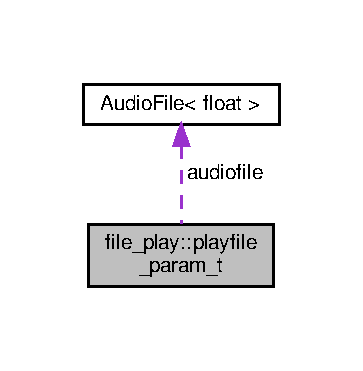
\includegraphics[width=174pt]{structfile__play_1_1playfile__param__t__coll__graph}
\end{center}
\end{figure}
\subsection*{Public Attributes}
\begin{DoxyCompactItemize}
\item 
\mbox{\Hypertarget{structfile__play_1_1playfile__param__t_a4cd8a16e1ad9bd8c462bd4b2fd9d7242}\label{structfile__play_1_1playfile__param__t_a4cd8a16e1ad9bd8c462bd4b2fd9d7242}} 
int {\bfseries reset}
\item 
\mbox{\Hypertarget{structfile__play_1_1playfile__param__t_aa861e2375a83bb4a20c175fa82b2b227}\label{structfile__play_1_1playfile__param__t_aa861e2375a83bb4a20c175fa82b2b227}} 
int {\bfseries play}
\item 
\mbox{\Hypertarget{structfile__play_1_1playfile__param__t_a91b362cb97d65ba95b453469515243ed}\label{structfile__play_1_1playfile__param__t_a91b362cb97d65ba95b453469515243ed}} 
int {\bfseries repeat}
\item 
\mbox{\Hypertarget{structfile__play_1_1playfile__param__t_a37f40197ccb20277f79d16d9c14359f8}\label{structfile__play_1_1playfile__param__t_a37f40197ccb20277f79d16d9c14359f8}} 
int {\bfseries current\+\_\+position\+\_\+l}
\item 
\mbox{\Hypertarget{structfile__play_1_1playfile__param__t_aa8b2c7aa5c332fdc76fa37d9d9848aad}\label{structfile__play_1_1playfile__param__t_aa8b2c7aa5c332fdc76fa37d9d9848aad}} 
int {\bfseries current\+\_\+position\+\_\+r}
\item 
\mbox{\Hypertarget{structfile__play_1_1playfile__param__t_acf92d55c66df1bb9b48439e0c1e79cf8}\label{structfile__play_1_1playfile__param__t_acf92d55c66df1bb9b48439e0c1e79cf8}} 
int {\bfseries num\+Samples}
\item 
\mbox{\Hypertarget{structfile__play_1_1playfile__param__t_a0f4fabcfbbee96f2dcf821209ef911f6}\label{structfile__play_1_1playfile__param__t_a0f4fabcfbbee96f2dcf821209ef911f6}} 
bool {\bfseries finish}
\item 
\mbox{\Hypertarget{structfile__play_1_1playfile__param__t_ac4be30af47c7f8c288a52238cae89ac9}\label{structfile__play_1_1playfile__param__t_ac4be30af47c7f8c288a52238cae89ac9}} 
int {\bfseries mono}
\item 
\mbox{\Hypertarget{structfile__play_1_1playfile__param__t_a16c994370868737c1679d36ce32db427}\label{structfile__play_1_1playfile__param__t_a16c994370868737c1679d36ce32db427}} 
std\+::string {\bfseries filename}
\item 
\mbox{\Hypertarget{structfile__play_1_1playfile__param__t_a5864aa1b0900ea84406f3548f95c38b5}\label{structfile__play_1_1playfile__param__t_a5864aa1b0900ea84406f3548f95c38b5}} 
\hyperlink{classAudioFile}{Audio\+File}$<$ float $>$ $\ast$ {\bfseries audiofile}
\end{DoxyCompactItemize}


\subsection{Detailed Description}


Definition at line 14 of file playfile.\+h.



The documentation for this struct was generated from the following file\+:\begin{DoxyCompactItemize}
\item 
playfile.\+h\end{DoxyCompactItemize}

\hypertarget{classpolyphase__hb__downsampler}{}\section{polyphase\+\_\+hb\+\_\+downsampler Class Reference}
\label{classpolyphase__hb__downsampler}\index{polyphase\+\_\+hb\+\_\+downsampler@{polyphase\+\_\+hb\+\_\+downsampler}}
\subsection*{Public Member Functions}
\begin{DoxyCompactItemize}
\item 
\mbox{\Hypertarget{classpolyphase__hb__downsampler_a9c929549928b7e325e7432b5172d1246}\label{classpolyphase__hb__downsampler_a9c929549928b7e325e7432b5172d1246}} 
{\bfseries polyphase\+\_\+hb\+\_\+downsampler} (float $\ast$filter\+\_\+taps, size\+\_\+t num\+\_\+taps, size\+\_\+t max\+\_\+frame\+\_\+size)
\item 
\mbox{\Hypertarget{classpolyphase__hb__downsampler_a7388f8a7fa60d315faddd9ca196644ee}\label{classpolyphase__hb__downsampler_a7388f8a7fa60d315faddd9ca196644ee}} 
void {\bfseries process} (float $\ast$in, float $\ast$out, size\+\_\+t frame\+\_\+size)
\end{DoxyCompactItemize}


\subsection{Detailed Description}


Definition at line 13 of file polyphase\+\_\+hb\+\_\+downsampler.\+h.



The documentation for this class was generated from the following files\+:\begin{DoxyCompactItemize}
\item 
polyphase\+\_\+hb\+\_\+downsampler.\+h\item 
polyphase\+\_\+hb\+\_\+downsampler.\+cpp\end{DoxyCompactItemize}

\hypertarget{classpolyphase__hb__upsampler}{}\section{polyphase\+\_\+hb\+\_\+upsampler Class Reference}
\label{classpolyphase__hb__upsampler}\index{polyphase\+\_\+hb\+\_\+upsampler@{polyphase\+\_\+hb\+\_\+upsampler}}
\subsection*{Public Member Functions}
\begin{DoxyCompactItemize}
\item 
\mbox{\Hypertarget{classpolyphase__hb__upsampler_ac703c7fd2eca07a979ba46f732e8133f}\label{classpolyphase__hb__upsampler_ac703c7fd2eca07a979ba46f732e8133f}} 
{\bfseries polyphase\+\_\+hb\+\_\+upsampler} (float $\ast$filter\+\_\+taps, size\+\_\+t num\+\_\+taps, size\+\_\+t max\+\_\+frame\+\_\+size)
\item 
\mbox{\Hypertarget{classpolyphase__hb__upsampler_a97fdd44f1c426eed9671146274a29b56}\label{classpolyphase__hb__upsampler_a97fdd44f1c426eed9671146274a29b56}} 
void {\bfseries process} (float $\ast$in, float $\ast$out, size\+\_\+t frame\+\_\+size)
\end{DoxyCompactItemize}


\subsection{Detailed Description}


Definition at line 12 of file polyphase\+\_\+hb\+\_\+upsampler.\+h.



The documentation for this class was generated from the following files\+:\begin{DoxyCompactItemize}
\item 
polyphase\+\_\+hb\+\_\+upsampler.\+h\item 
polyphase\+\_\+hb\+\_\+upsampler.\+cpp\end{DoxyCompactItemize}

\hypertarget{classresample}{}\section{resample Class Reference}
\label{classresample}\index{resample@{resample}}


Resample Class.  




{\ttfamily \#include $<$resample.\+hpp$>$}

\subsection*{Public Member Functions}
\begin{DoxyCompactItemize}
\item 
\hyperlink{classresample_af9ae60e50b2be5ee96f8f2bddf942b90}{resample} (float $\ast$taps, size\+\_\+t tap\+\_\+size, size\+\_\+t max\+\_\+in\+\_\+buf\+\_\+size, int interp\+\_\+factor, int deci\+\_\+factor)
\begin{DoxyCompactList}\small\item\em Resample constructor. \end{DoxyCompactList}\item 
\mbox{\Hypertarget{classresample_a98884fd6264cbd4c7254e7c3767b5a85}\label{classresample_a98884fd6264cbd4c7254e7c3767b5a85}} 
\hyperlink{classresample_a98884fd6264cbd4c7254e7c3767b5a85}{$\sim$resample} ()
\begin{DoxyCompactList}\small\item\em Resample destructor. \end{DoxyCompactList}\item 
void \hyperlink{classresample_a121c622a3ed64b69b09025a008f84dc3}{resamp} (float $\ast$data\+\_\+in, size\+\_\+t in\+\_\+size, float $\ast$data\+\_\+out, size\+\_\+t $\ast$out\+\_\+size)
\begin{DoxyCompactList}\small\item\em Getting the resampled signal. \end{DoxyCompactList}\end{DoxyCompactItemize}


\subsection{Detailed Description}
Resample Class. 

Resampling class implements L/\+M-\/fold resampling 

Definition at line 15 of file resample.\+hpp.



\subsection{Constructor \& Destructor Documentation}
\mbox{\Hypertarget{classresample_af9ae60e50b2be5ee96f8f2bddf942b90}\label{classresample_af9ae60e50b2be5ee96f8f2bddf942b90}} 
\index{resample@{resample}!resample@{resample}}
\index{resample@{resample}!resample@{resample}}
\subsubsection{\texorpdfstring{resample()}{resample()}}
{\footnotesize\ttfamily resample\+::resample (\begin{DoxyParamCaption}\item[{float $\ast$}]{taps,  }\item[{size\+\_\+t}]{tap\+\_\+size,  }\item[{size\+\_\+t}]{max\+\_\+in\+\_\+buf\+\_\+size,  }\item[{int}]{interp\+\_\+factor,  }\item[{int}]{deci\+\_\+factor }\end{DoxyParamCaption})\hspace{0.3cm}{\ttfamily [explicit]}}



Resample constructor. 


\begin{DoxyParams}[1]{Parameters}
\mbox{\tt in}  & {\em taps} & The filter taps of the lowpass filter (to reject images and prevent aliasing) \\
\hline
\mbox{\tt in}  & {\em tap\+\_\+size} & The number of taps of the lowpass filter \\
\hline
\mbox{\tt in}  & {\em max\+\_\+in\+\_\+buf\+\_\+size} & The maximum input buffer size \\
\hline
\mbox{\tt in}  & {\em interp\+\_\+factor} & The interpolation factor L (to implement L-\/fold expander) \\
\hline
\mbox{\tt in}  & {\em deci\+\_\+factor} & The decimation factor M (to implement M-\/fold decimator) \\
\hline
\end{DoxyParams}


Definition at line 7 of file resample.\+cpp.



\subsection{Member Function Documentation}
\mbox{\Hypertarget{classresample_a121c622a3ed64b69b09025a008f84dc3}\label{classresample_a121c622a3ed64b69b09025a008f84dc3}} 
\index{resample@{resample}!resamp@{resamp}}
\index{resamp@{resamp}!resample@{resample}}
\subsubsection{\texorpdfstring{resamp()}{resamp()}}
{\footnotesize\ttfamily void resample\+::resamp (\begin{DoxyParamCaption}\item[{float $\ast$}]{data\+\_\+in,  }\item[{size\+\_\+t}]{in\+\_\+size,  }\item[{float $\ast$}]{data\+\_\+out,  }\item[{size\+\_\+t $\ast$}]{out\+\_\+size }\end{DoxyParamCaption})}



Getting the resampled signal. 


\begin{DoxyParams}[1]{Parameters}
\mbox{\tt in}  & {\em data\+\_\+in} & The signal in original sampling rate \\
\hline
\mbox{\tt in}  & {\em in\+\_\+size} & The size of the original signal \\
\hline
\mbox{\tt out}  & {\em data\+\_\+out} & The resampled signal \\
\hline
\mbox{\tt out}  & {\em out\+\_\+size} & The size of the resampled signal \\
\hline
\end{DoxyParams}


Definition at line 23 of file resample.\+cpp.



The documentation for this class was generated from the following files\+:\begin{DoxyCompactItemize}
\item 
resample.\+hpp\item 
resample.\+cpp\end{DoxyCompactItemize}

\hypertarget{structrk__sema}{}\section{rk\+\_\+sema Struct Reference}
\label{structrk__sema}\index{rk\+\_\+sema@{rk\+\_\+sema}}
\subsection*{Public Attributes}
\begin{DoxyCompactItemize}
\item 
\mbox{\Hypertarget{structrk__sema_aa1a0c0c37646f85eb88bca7c48e7c5a3}\label{structrk__sema_aa1a0c0c37646f85eb88bca7c48e7c5a3}} 
sem\+\_\+t {\bfseries sem}
\end{DoxyCompactItemize}


\subsection{Detailed Description}


Definition at line 8 of file sema.\+hpp.



The documentation for this struct was generated from the following file\+:\begin{DoxyCompactItemize}
\item 
sema.\+hpp\end{DoxyCompactItemize}

\hypertarget{classtenband__filterbank}{}\section{tenband\+\_\+filterbank Class Reference}
\label{classtenband__filterbank}\index{tenband\+\_\+filterbank@{tenband\+\_\+filterbank}}


The Ten Band Filter bank is a 10 Band Multirate Filter Bank with its center frequencies located at 250\+Hz, 500\+Hz, 750\+Hz, 1k\+Hz, 1.\+5k\+Hz, 2k\+Hz, 3k\+Hz, 4k\+Hz, 6k\+Hz, 8k\+Hz.  




{\ttfamily \#include $<$tenband\+\_\+filterbank.\+h$>$}

\subsection*{Public Member Functions}
\begin{DoxyCompactItemize}
\item 
\hyperlink{classtenband__filterbank_ab256b89ab03136482f899b7d821369b6}{tenband\+\_\+filterbank} (size\+\_\+t max\+\_\+frame\+\_\+size, bool aligned)
\begin{DoxyCompactList}\small\item\em The consturctor for the Ten Band Filter bank. \end{DoxyCompactList}\item 
\mbox{\Hypertarget{classtenband__filterbank_a1a197b127d5f9a0e7a8c964d0aad24af}\label{classtenband__filterbank_a1a197b127d5f9a0e7a8c964d0aad24af}} 
\hyperlink{classtenband__filterbank_a1a197b127d5f9a0e7a8c964d0aad24af}{$\sim$tenband\+\_\+filterbank} ()
\begin{DoxyCompactList}\small\item\em The desturctor for the Ten Band Filter bank. \end{DoxyCompactList}\item 
void \hyperlink{classtenband__filterbank_a2368544882712253bb5c220cc4517bd4}{process} (float $\ast$in, float $\ast$$\ast$out, size\+\_\+t frame\+\_\+size)
\begin{DoxyCompactList}\small\item\em This function decomposes the incoming frame of data into the 10 subbands. \end{DoxyCompactList}\item 
void \hyperlink{classtenband__filterbank_a170a3e7896129748d8b33b7adbf44866}{set} (bool aligned)
\begin{DoxyCompactList}\small\item\em The compensation for the various group delay can be toggled on and off live. \end{DoxyCompactList}\item 
void \hyperlink{classtenband__filterbank_a1bc3d0099acfa8cabccccdec579abeed}{get} (bool \&aligned)
\begin{DoxyCompactList}\small\item\em Used to read the current status of the aligned variable. \end{DoxyCompactList}\end{DoxyCompactItemize}


\subsection{Detailed Description}
The Ten Band Filter bank is a 10 Band Multirate Filter Bank with its center frequencies located at 250\+Hz, 500\+Hz, 750\+Hz, 1k\+Hz, 1.\+5k\+Hz, 2k\+Hz, 3k\+Hz, 4k\+Hz, 6k\+Hz, 8k\+Hz. 

Definition at line 44 of file tenband\+\_\+filterbank.\+h.



\subsection{Constructor \& Destructor Documentation}
\mbox{\Hypertarget{classtenband__filterbank_ab256b89ab03136482f899b7d821369b6}\label{classtenband__filterbank_ab256b89ab03136482f899b7d821369b6}} 
\index{tenband\+\_\+filterbank@{tenband\+\_\+filterbank}!tenband\+\_\+filterbank@{tenband\+\_\+filterbank}}
\index{tenband\+\_\+filterbank@{tenband\+\_\+filterbank}!tenband\+\_\+filterbank@{tenband\+\_\+filterbank}}
\subsubsection{\texorpdfstring{tenband\+\_\+filterbank()}{tenband\_filterbank()}}
{\footnotesize\ttfamily tenband\+\_\+filterbank\+::tenband\+\_\+filterbank (\begin{DoxyParamCaption}\item[{size\+\_\+t}]{max\+\_\+frame\+\_\+size,  }\item[{bool}]{aligned }\end{DoxyParamCaption})}



The consturctor for the Ten Band Filter bank. 


\begin{DoxyParams}{Parameters}
{\em max\+\_\+frame\+\_\+size} & \mbox{[}in\mbox{]} -\/ The maximum size of buffer that would need to be processed at any time step. \\
\hline
{\em aligned} & \mbox{[}in\mbox{]} -\/ Enabling the delay blocks to compensate for the various group delays. \\
\hline
\end{DoxyParams}


Definition at line 31 of file tenband\+\_\+filterbank.\+cpp.



\subsection{Member Function Documentation}
\mbox{\Hypertarget{classtenband__filterbank_a1bc3d0099acfa8cabccccdec579abeed}\label{classtenband__filterbank_a1bc3d0099acfa8cabccccdec579abeed}} 
\index{tenband\+\_\+filterbank@{tenband\+\_\+filterbank}!get@{get}}
\index{get@{get}!tenband\+\_\+filterbank@{tenband\+\_\+filterbank}}
\subsubsection{\texorpdfstring{get()}{get()}}
{\footnotesize\ttfamily void tenband\+\_\+filterbank\+::get (\begin{DoxyParamCaption}\item[{bool \&}]{aligned }\end{DoxyParamCaption})}



Used to read the current status of the aligned variable. 


\begin{DoxyParams}[1]{Parameters}
\mbox{\tt out}  & {\em aligned} & Grabbing the current status of the aligned variable. \\
\hline
\end{DoxyParams}


Definition at line 200 of file tenband\+\_\+filterbank.\+cpp.

\mbox{\Hypertarget{classtenband__filterbank_a2368544882712253bb5c220cc4517bd4}\label{classtenband__filterbank_a2368544882712253bb5c220cc4517bd4}} 
\index{tenband\+\_\+filterbank@{tenband\+\_\+filterbank}!process@{process}}
\index{process@{process}!tenband\+\_\+filterbank@{tenband\+\_\+filterbank}}
\subsubsection{\texorpdfstring{process()}{process()}}
{\footnotesize\ttfamily void tenband\+\_\+filterbank\+::process (\begin{DoxyParamCaption}\item[{float $\ast$}]{in,  }\item[{float $\ast$$\ast$}]{out,  }\item[{size\+\_\+t}]{frame\+\_\+size }\end{DoxyParamCaption})}



This function decomposes the incoming frame of data into the 10 subbands. 


\begin{DoxyParams}[1]{Parameters}
\mbox{\tt in}  & {\em in} & An array of data the size of frame\+\_\+size. \\
\hline
\mbox{\tt out}  & {\em out} & A 2D 10 by frame\+\_\+size array of data for the 10 subbands \\
\hline
\mbox{\tt in}  & {\em frame\+\_\+size} & The amount of data contained in the incoming array. \\
\hline
\end{DoxyParams}


Definition at line 150 of file tenband\+\_\+filterbank.\+cpp.

\mbox{\Hypertarget{classtenband__filterbank_a170a3e7896129748d8b33b7adbf44866}\label{classtenband__filterbank_a170a3e7896129748d8b33b7adbf44866}} 
\index{tenband\+\_\+filterbank@{tenband\+\_\+filterbank}!set@{set}}
\index{set@{set}!tenband\+\_\+filterbank@{tenband\+\_\+filterbank}}
\subsubsection{\texorpdfstring{set()}{set()}}
{\footnotesize\ttfamily void tenband\+\_\+filterbank\+::set (\begin{DoxyParamCaption}\item[{bool}]{aligned }\end{DoxyParamCaption})}



The compensation for the various group delay can be toggled on and off live. 


\begin{DoxyParams}[1]{Parameters}
\mbox{\tt in}  & {\em aligned} & Enabling the delay blocks to compensate for the various group delays. \\
\hline
\end{DoxyParams}


Definition at line 197 of file tenband\+\_\+filterbank.\+cpp.



The documentation for this class was generated from the following files\+:\begin{DoxyCompactItemize}
\item 
tenband\+\_\+filterbank.\+h\item 
tenband\+\_\+filterbank.\+cpp\end{DoxyCompactItemize}

\hypertarget{classwdrc}{}\section{wdrc Class Reference}
\label{classwdrc}\index{wdrc@{wdrc}}


Wide Dynamic Range Compression (W\+D\+RC) Class.  




{\ttfamily \#include $<$wdrc.\+hpp$>$}

\subsection*{Public Member Functions}
\begin{DoxyCompactItemize}
\item 
\hyperlink{classwdrc_a9a836480fcfd49a21f592d15ef94f290}{wdrc} (float gain50, float gain80, float knee\+\_\+low, float mpo\+\_\+limit)
\begin{DoxyCompactList}\small\item\em wdrc constructor \end{DoxyCompactList}\item 
\mbox{\Hypertarget{classwdrc_ab99f98ae700777e0505ff3460d107a21}\label{classwdrc_ab99f98ae700777e0505ff3460d107a21}} 
\hyperlink{classwdrc_ab99f98ae700777e0505ff3460d107a21}{$\sim$wdrc} ()
\begin{DoxyCompactList}\small\item\em wdrc destructor \end{DoxyCompactList}\item 
void \hyperlink{classwdrc_a8b804984f0b23d2883f5653e42570caf}{set\+\_\+param} (float gain50, float gain80, float knee\+\_\+low, float mpo\+\_\+limit)
\begin{DoxyCompactList}\small\item\em Setting W\+D\+RC parameters. \end{DoxyCompactList}\item 
void \hyperlink{classwdrc_a9365c99f1d0b4a706dd031d4093922cd}{get\+\_\+param} (float \&gain50, float \&gain80, float \&knee\+\_\+low, float \&mpo\+\_\+limit)
\begin{DoxyCompactList}\small\item\em Getting W\+D\+RC parameters. \end{DoxyCompactList}\item 
void \hyperlink{classwdrc_abc022a485b25b994d226053021224e31}{process} (float $\ast$input, float $\ast$pdb, size\+\_\+t in\+\_\+len, float $\ast$output)
\begin{DoxyCompactList}\small\item\em Perform W\+D\+RC. \end{DoxyCompactList}\end{DoxyCompactItemize}


\subsection{Detailed Description}
Wide Dynamic Range Compression (W\+D\+RC) Class. 

Applying W\+D\+RC to a subband signal from an analysis filterbank 

Definition at line 18 of file wdrc.\+hpp.



\subsection{Constructor \& Destructor Documentation}
\mbox{\Hypertarget{classwdrc_a9a836480fcfd49a21f592d15ef94f290}\label{classwdrc_a9a836480fcfd49a21f592d15ef94f290}} 
\index{wdrc@{wdrc}!wdrc@{wdrc}}
\index{wdrc@{wdrc}!wdrc@{wdrc}}
\subsubsection{\texorpdfstring{wdrc()}{wdrc()}}
{\footnotesize\ttfamily wdrc\+::wdrc (\begin{DoxyParamCaption}\item[{float}]{gain50,  }\item[{float}]{gain80,  }\item[{float}]{knee\+\_\+low,  }\item[{float}]{mpo\+\_\+limit }\end{DoxyParamCaption})\hspace{0.3cm}{\ttfamily [explicit]}}



wdrc constructor 


\begin{DoxyParams}[1]{Parameters}
\mbox{\tt in}  & {\em gain50} & Gain at 50 dB S\+PL of input level \\
\hline
\mbox{\tt in}  & {\em gain80} & Gain at 80 dB S\+PL of input level \\
\hline
\mbox{\tt in}  & {\em knee\+\_\+low} & Lower knee-\/point \\
\hline
\mbox{\tt in}  & {\em mpo\+\_\+limit} & Maximum power output (M\+PO) \\
\hline
\end{DoxyParams}


Definition at line 3 of file wdrc.\+cpp.



\subsection{Member Function Documentation}
\mbox{\Hypertarget{classwdrc_a9365c99f1d0b4a706dd031d4093922cd}\label{classwdrc_a9365c99f1d0b4a706dd031d4093922cd}} 
\index{wdrc@{wdrc}!get\+\_\+param@{get\+\_\+param}}
\index{get\+\_\+param@{get\+\_\+param}!wdrc@{wdrc}}
\subsubsection{\texorpdfstring{get\+\_\+param()}{get\_param()}}
{\footnotesize\ttfamily void wdrc\+::get\+\_\+param (\begin{DoxyParamCaption}\item[{float \&}]{gain50,  }\item[{float \&}]{gain80,  }\item[{float \&}]{knee\+\_\+low,  }\item[{float \&}]{mpo\+\_\+limit }\end{DoxyParamCaption})}



Getting W\+D\+RC parameters. 


\begin{DoxyParams}[1]{Parameters}
\mbox{\tt out}  & {\em gain50} & Gain at 50 dB S\+PL of input level \\
\hline
\mbox{\tt out}  & {\em gain80} & Gain at 80 dB S\+PL of input level \\
\hline
\mbox{\tt out}  & {\em knee\+\_\+low} & Lower knee-\/point \\
\hline
\mbox{\tt out}  & {\em mpo\+\_\+limit} & M\+PO \\
\hline
\end{DoxyParams}


Definition at line 43 of file wdrc.\+cpp.

\mbox{\Hypertarget{classwdrc_abc022a485b25b994d226053021224e31}\label{classwdrc_abc022a485b25b994d226053021224e31}} 
\index{wdrc@{wdrc}!process@{process}}
\index{process@{process}!wdrc@{wdrc}}
\subsubsection{\texorpdfstring{process()}{process()}}
{\footnotesize\ttfamily void wdrc\+::process (\begin{DoxyParamCaption}\item[{float $\ast$}]{input,  }\item[{float $\ast$}]{pdb,  }\item[{size\+\_\+t}]{in\+\_\+len,  }\item[{float $\ast$}]{output }\end{DoxyParamCaption})}



Perform W\+D\+RC. 

The peak detector output in dB S\+PL is needed as one of the inputs. The gain at 50 and 80 dB S\+PL is specified for the frequency sub-\/band, along with the lower and upper kneepoints in dB S\+PL. The compressor is linear below the lower kneepoint and applies compression limiting above the upper kneepoint 
\begin{DoxyParams}[1]{Parameters}
\mbox{\tt in}  & {\em input} & The input signal (1-\/D array) \\
\hline
\mbox{\tt in}  & {\em pdb} & The output from the peak detector in S\+PL, i.\+e., the output from get\+\_\+spl member function in \hyperlink{classpeak__detect}{peak\+\_\+detect} class \\
\hline
\mbox{\tt in}  & {\em in\+\_\+len} & Length of the input signal \\
\hline
\mbox{\tt out}  & {\em output} & Pointer to a signal (1-\/D array) where the compressed output of the subband signal will be written, i.\+e., the output of W\+D\+RC \\
\hline
\end{DoxyParams}
\begin{DoxySeeAlso}{See also}
\hyperlink{classpeak__detect}{peak\+\_\+detect} 
\end{DoxySeeAlso}


Definition at line 52 of file wdrc.\+cpp.

\mbox{\Hypertarget{classwdrc_a8b804984f0b23d2883f5653e42570caf}\label{classwdrc_a8b804984f0b23d2883f5653e42570caf}} 
\index{wdrc@{wdrc}!set\+\_\+param@{set\+\_\+param}}
\index{set\+\_\+param@{set\+\_\+param}!wdrc@{wdrc}}
\subsubsection{\texorpdfstring{set\+\_\+param()}{set\_param()}}
{\footnotesize\ttfamily void wdrc\+::set\+\_\+param (\begin{DoxyParamCaption}\item[{float}]{gain50,  }\item[{float}]{gain80,  }\item[{float}]{knee\+\_\+low,  }\item[{float}]{mpo\+\_\+limit }\end{DoxyParamCaption})}



Setting W\+D\+RC parameters. 


\begin{DoxyParams}[1]{Parameters}
\mbox{\tt in}  & {\em gain50} & Gain at 50 dB S\+PL of input level \\
\hline
\mbox{\tt in}  & {\em gain80} & Gain at 80 dB S\+PL of input level \\
\hline
\mbox{\tt in}  & {\em knee\+\_\+low} & Lower knee-\/point \\
\hline
\mbox{\tt in}  & {\em mpo\+\_\+limit} & M\+PO \\
\hline
\end{DoxyParams}


Definition at line 25 of file wdrc.\+cpp.



The documentation for this class was generated from the following files\+:\begin{DoxyCompactItemize}
\item 
wdrc.\+hpp\item 
wdrc.\+cpp\end{DoxyCompactItemize}

\chapter{File Documentation}
\hypertarget{adaptive__filter_8cpp}{}\section{adaptive\+\_\+filter.\+cpp File Reference}
\label{adaptive__filter_8cpp}\index{adaptive\+\_\+filter.\+cpp@{adaptive\+\_\+filter.\+cpp}}
{\ttfamily \#include $<$cmath$>$}\newline
{\ttfamily \#include $<$iostream$>$}\newline
{\ttfamily \#include $<$O\+S\+P/array\+\_\+utilities/array\+\_\+utilities.\+hpp$>$}\newline
{\ttfamily \#include $<$O\+S\+P/adaptive\+\_\+filter/adaptive\+\_\+filter.\+hpp$>$}\newline
Include dependency graph for adaptive\+\_\+filter.\+cpp\+:\nopagebreak
\begin{figure}[H]
\begin{center}
\leavevmode
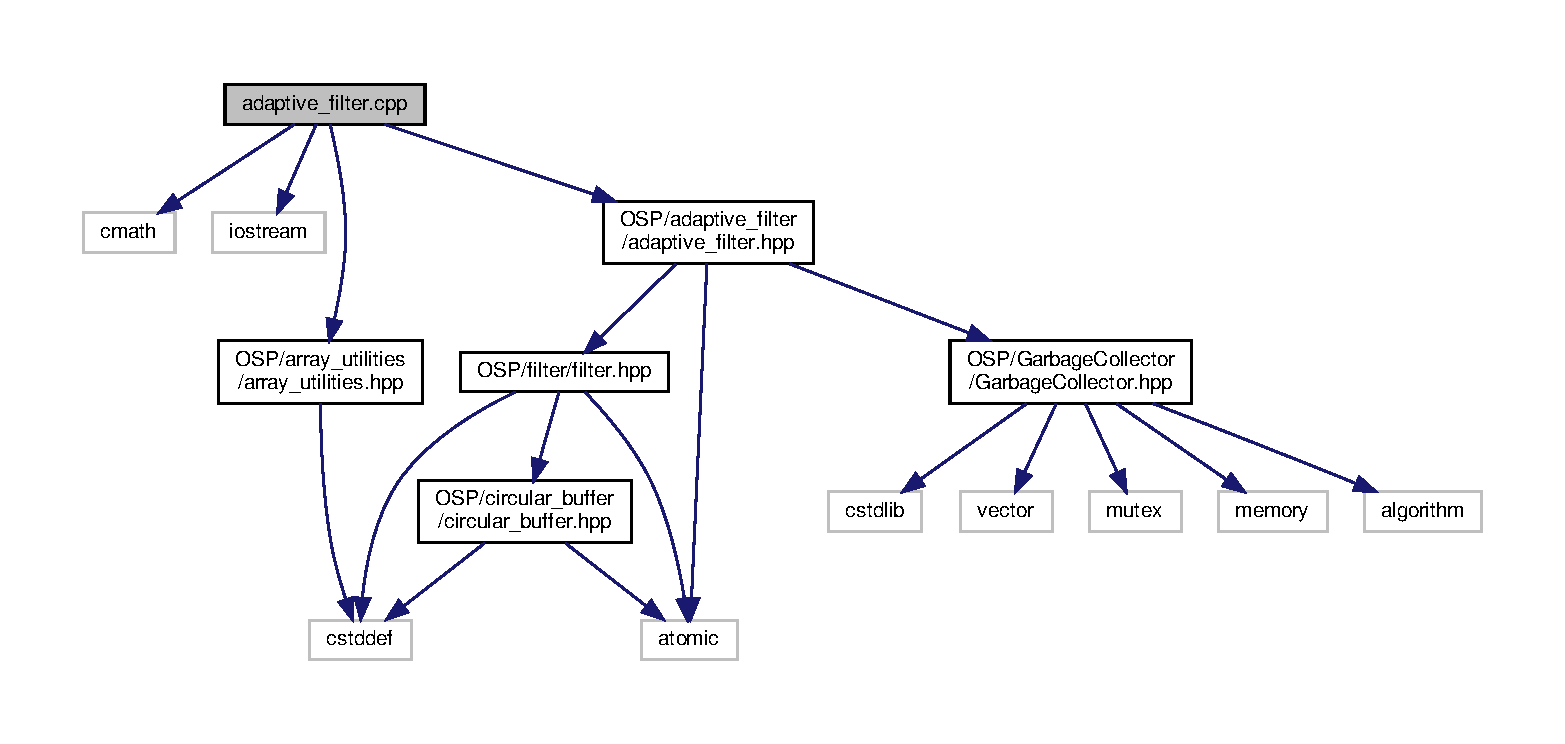
\includegraphics[width=350pt]{adaptive__filter_8cpp__incl}
\end{center}
\end{figure}


\subsection{Detailed Description}
\begin{DoxyAuthor}{Author}
Open Speech Platform (O\+SP) Team, U\+C\+SD 
\end{DoxyAuthor}
\begin{DoxyCopyright}{Copyright}
Copyright (C) 2020 Regents of the University of California Redistribution and use in source and binary forms, with or without modification, are permitted provided that the following conditions are met\+: \begin{DoxyVerb}1. Redistributions of source code must retain the above copyright notice, this list of conditions and the
following disclaimer.

2. Redistributions in binary form must reproduce the above copyright notice, this list of conditions and the
following disclaimer in the documentation and/or other materials provided with the distribution.
\end{DoxyVerb}

\end{DoxyCopyright}
T\+H\+IS S\+O\+F\+T\+W\+A\+RE IS P\+R\+O\+V\+I\+D\+ED BY T\+HE C\+O\+P\+Y\+R\+I\+G\+HT H\+O\+L\+D\+E\+RS A\+ND C\+O\+N\+T\+R\+I\+B\+U\+T\+O\+RS \char`\"{}\+A\+S I\+S\char`\"{} A\+ND A\+NY E\+X\+P\+R\+E\+SS OR I\+M\+P\+L\+I\+ED W\+A\+R\+R\+A\+N\+T\+I\+ES, I\+N\+C\+L\+U\+D\+I\+NG, B\+UT N\+OT L\+I\+M\+I\+T\+ED TO, T\+HE I\+M\+P\+L\+I\+ED W\+A\+R\+R\+A\+N\+T\+I\+ES OF M\+E\+R\+C\+H\+A\+N\+T\+A\+B\+I\+L\+I\+TY A\+ND F\+I\+T\+N\+E\+SS F\+OR A P\+A\+R\+T\+I\+C\+U\+L\+AR P\+U\+R\+P\+O\+SE A\+RE D\+I\+S\+C\+L\+A\+I\+M\+ED. IN NO E\+V\+E\+NT S\+H\+A\+LL T\+HE C\+O\+P\+Y\+R\+I\+G\+HT H\+O\+L\+D\+ER OR C\+O\+N\+T\+R\+I\+B\+U\+T\+O\+RS BE L\+I\+A\+B\+LE F\+OR A\+NY D\+I\+R\+E\+CT, I\+N\+D\+I\+R\+E\+CT, I\+N\+C\+I\+D\+E\+N\+T\+AL, S\+P\+E\+C\+I\+AL, E\+X\+E\+M\+P\+L\+A\+RY, OR C\+O\+N\+S\+E\+Q\+U\+E\+N\+T\+I\+AL D\+A\+M\+A\+G\+ES (I\+N\+C\+L\+U\+D\+I\+NG, B\+UT N\+OT L\+I\+M\+I\+T\+ED TO, P\+R\+O\+C\+U\+R\+E\+M\+E\+NT OF S\+U\+B\+S\+T\+I\+T\+U\+TE G\+O\+O\+DS OR S\+E\+R\+V\+I\+C\+ES; L\+O\+SS OF U\+SE, D\+A\+TA, OR P\+R\+O\+F\+I\+TS; OR B\+U\+S\+I\+N\+E\+SS I\+N\+T\+E\+R\+R\+U\+P\+T\+I\+ON) H\+O\+W\+E\+V\+ER C\+A\+U\+S\+ED A\+ND ON A\+NY T\+H\+E\+O\+RY OF L\+I\+A\+B\+I\+L\+I\+TY, W\+H\+E\+T\+H\+ER IN C\+O\+N\+T\+R\+A\+CT, S\+T\+R\+I\+CT L\+I\+A\+B\+I\+L\+I\+TY, OR T\+O\+RT (I\+N\+C\+L\+U\+D\+I\+NG N\+E\+G\+L\+I\+G\+E\+N\+CE OR O\+T\+H\+E\+R\+W\+I\+SE) A\+R\+I\+S\+I\+NG IN A\+NY W\+AY O\+UT OF T\+HE U\+SE OF T\+H\+IS S\+O\+F\+T\+W\+A\+RE, E\+V\+EN IF A\+D\+V\+I\+S\+ED OF T\+HE P\+O\+S\+S\+I\+B\+I\+L\+I\+TY OF S\+U\+CH D\+A\+M\+A\+GE. 
\hypertarget{adaptive__filter_8hpp}{}\section{adaptive\+\_\+filter.\+hpp File Reference}
\label{adaptive__filter_8hpp}\index{adaptive\+\_\+filter.\+hpp@{adaptive\+\_\+filter.\+hpp}}
{\ttfamily \#include $<$O\+S\+P/filter/filter.\+hpp$>$}\newline
{\ttfamily \#include $<$atomic$>$}\newline
{\ttfamily \#include $<$O\+S\+P/\+Garbage\+Collector/\+Garbage\+Collector.\+hpp$>$}\newline
Include dependency graph for adaptive\+\_\+filter.\+hpp\+:\nopagebreak
\begin{figure}[H]
\begin{center}
\leavevmode
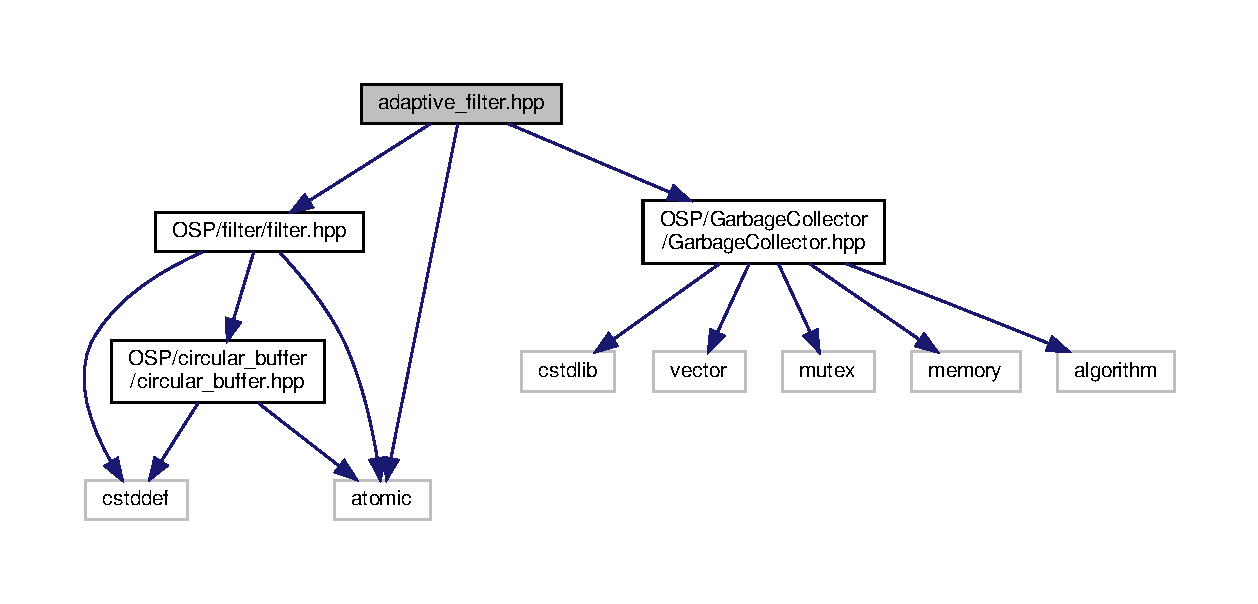
\includegraphics[width=350pt]{adaptive__filter_8hpp__incl}
\end{center}
\end{figure}
This graph shows which files directly or indirectly include this file\+:\nopagebreak
\begin{figure}[H]
\begin{center}
\leavevmode
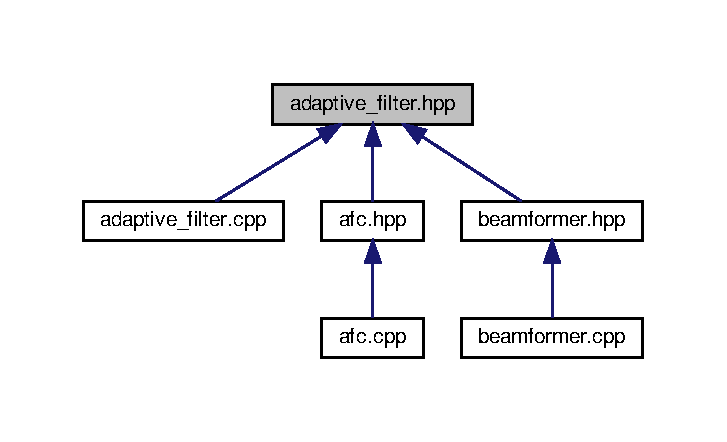
\includegraphics[width=349pt]{adaptive__filter_8hpp__dep__incl}
\end{center}
\end{figure}
\subsection*{Classes}
\begin{DoxyCompactItemize}
\item 
class \hyperlink{classadaptive__filter}{adaptive\+\_\+filter}
\begin{DoxyCompactList}\small\item\em Adaptive Filter Class. \end{DoxyCompactList}\end{DoxyCompactItemize}


\subsection{Detailed Description}
\begin{DoxyAuthor}{Author}
Open Speech Platform (O\+SP) Team, U\+C\+SD 
\end{DoxyAuthor}
\begin{DoxyCopyright}{Copyright}
Copyright (C) 2020 Regents of the University of California Redistribution and use in source and binary forms, with or without modification, are permitted provided that the following conditions are met\+: \begin{DoxyVerb}1. Redistributions of source code must retain the above copyright notice, this list of conditions and the
following disclaimer.

2. Redistributions in binary form must reproduce the above copyright notice, this list of conditions and the
following disclaimer in the documentation and/or other materials provided with the distribution.
\end{DoxyVerb}

\end{DoxyCopyright}
T\+H\+IS S\+O\+F\+T\+W\+A\+RE IS P\+R\+O\+V\+I\+D\+ED BY T\+HE C\+O\+P\+Y\+R\+I\+G\+HT H\+O\+L\+D\+E\+RS A\+ND C\+O\+N\+T\+R\+I\+B\+U\+T\+O\+RS \char`\"{}\+A\+S I\+S\char`\"{} A\+ND A\+NY E\+X\+P\+R\+E\+SS OR I\+M\+P\+L\+I\+ED W\+A\+R\+R\+A\+N\+T\+I\+ES, I\+N\+C\+L\+U\+D\+I\+NG, B\+UT N\+OT L\+I\+M\+I\+T\+ED TO, T\+HE I\+M\+P\+L\+I\+ED W\+A\+R\+R\+A\+N\+T\+I\+ES OF M\+E\+R\+C\+H\+A\+N\+T\+A\+B\+I\+L\+I\+TY A\+ND F\+I\+T\+N\+E\+SS F\+OR A P\+A\+R\+T\+I\+C\+U\+L\+AR P\+U\+R\+P\+O\+SE A\+RE D\+I\+S\+C\+L\+A\+I\+M\+ED. IN NO E\+V\+E\+NT S\+H\+A\+LL T\+HE C\+O\+P\+Y\+R\+I\+G\+HT H\+O\+L\+D\+ER OR C\+O\+N\+T\+R\+I\+B\+U\+T\+O\+RS BE L\+I\+A\+B\+LE F\+OR A\+NY D\+I\+R\+E\+CT, I\+N\+D\+I\+R\+E\+CT, I\+N\+C\+I\+D\+E\+N\+T\+AL, S\+P\+E\+C\+I\+AL, E\+X\+E\+M\+P\+L\+A\+RY, OR C\+O\+N\+S\+E\+Q\+U\+E\+N\+T\+I\+AL D\+A\+M\+A\+G\+ES (I\+N\+C\+L\+U\+D\+I\+NG, B\+UT N\+OT L\+I\+M\+I\+T\+ED TO, P\+R\+O\+C\+U\+R\+E\+M\+E\+NT OF S\+U\+B\+S\+T\+I\+T\+U\+TE G\+O\+O\+DS OR S\+E\+R\+V\+I\+C\+ES; L\+O\+SS OF U\+SE, D\+A\+TA, OR P\+R\+O\+F\+I\+TS; OR B\+U\+S\+I\+N\+E\+SS I\+N\+T\+E\+R\+R\+U\+P\+T\+I\+ON) H\+O\+W\+E\+V\+ER C\+A\+U\+S\+ED A\+ND ON A\+NY T\+H\+E\+O\+RY OF L\+I\+A\+B\+I\+L\+I\+TY, W\+H\+E\+T\+H\+ER IN C\+O\+N\+T\+R\+A\+CT, S\+T\+R\+I\+CT L\+I\+A\+B\+I\+L\+I\+TY, OR T\+O\+RT (I\+N\+C\+L\+U\+D\+I\+NG N\+E\+G\+L\+I\+G\+E\+N\+CE OR O\+T\+H\+E\+R\+W\+I\+SE) A\+R\+I\+S\+I\+NG IN A\+NY W\+AY O\+UT OF T\+HE U\+SE OF T\+H\+IS S\+O\+F\+T\+W\+A\+RE, E\+V\+EN IF A\+D\+V\+I\+S\+ED OF T\+HE P\+O\+S\+S\+I\+B\+I\+L\+I\+TY OF S\+U\+CH D\+A\+M\+A\+GE. 
\hypertarget{afc_8cpp}{}\section{afc.\+cpp File Reference}
\label{afc_8cpp}\index{afc.\+cpp@{afc.\+cpp}}
{\ttfamily \#include $<$O\+S\+P/afc/afc.\+hpp$>$}\newline
Include dependency graph for afc.\+cpp\+:\nopagebreak
\begin{figure}[H]
\begin{center}
\leavevmode
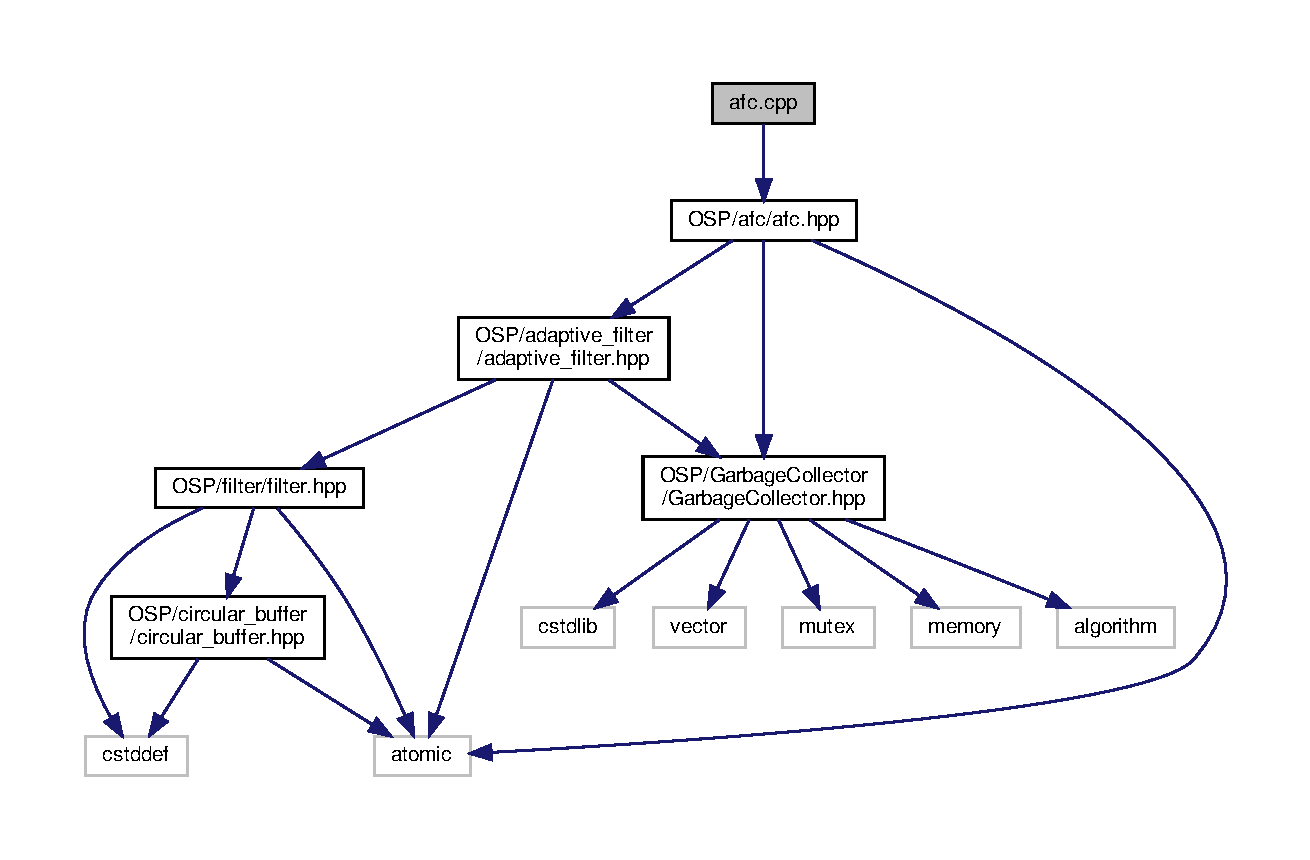
\includegraphics[width=350pt]{afc_8cpp__incl}
\end{center}
\end{figure}


\subsection{Detailed Description}
\begin{DoxyAuthor}{Author}
Open Speech Platform (O\+SP) Team, U\+C\+SD 
\end{DoxyAuthor}
\begin{DoxyCopyright}{Copyright}
Copyright (C) 2020 Regents of the University of California Redistribution and use in source and binary forms, with or without modification, are permitted provided that the following conditions are met\+: \begin{DoxyVerb}1. Redistributions of source code must retain the above copyright notice, this list of conditions and the
following disclaimer.

2. Redistributions in binary form must reproduce the above copyright notice, this list of conditions and the
following disclaimer in the documentation and/or other materials provided with the distribution.
\end{DoxyVerb}

\end{DoxyCopyright}
T\+H\+IS S\+O\+F\+T\+W\+A\+RE IS P\+R\+O\+V\+I\+D\+ED BY T\+HE C\+O\+P\+Y\+R\+I\+G\+HT H\+O\+L\+D\+E\+RS A\+ND C\+O\+N\+T\+R\+I\+B\+U\+T\+O\+RS \char`\"{}\+A\+S I\+S\char`\"{} A\+ND A\+NY E\+X\+P\+R\+E\+SS OR I\+M\+P\+L\+I\+ED W\+A\+R\+R\+A\+N\+T\+I\+ES, I\+N\+C\+L\+U\+D\+I\+NG, B\+UT N\+OT L\+I\+M\+I\+T\+ED TO, T\+HE I\+M\+P\+L\+I\+ED W\+A\+R\+R\+A\+N\+T\+I\+ES OF M\+E\+R\+C\+H\+A\+N\+T\+A\+B\+I\+L\+I\+TY A\+ND F\+I\+T\+N\+E\+SS F\+OR A P\+A\+R\+T\+I\+C\+U\+L\+AR P\+U\+R\+P\+O\+SE A\+RE D\+I\+S\+C\+L\+A\+I\+M\+ED. IN NO E\+V\+E\+NT S\+H\+A\+LL T\+HE C\+O\+P\+Y\+R\+I\+G\+HT H\+O\+L\+D\+ER OR C\+O\+N\+T\+R\+I\+B\+U\+T\+O\+RS BE L\+I\+A\+B\+LE F\+OR A\+NY D\+I\+R\+E\+CT, I\+N\+D\+I\+R\+E\+CT, I\+N\+C\+I\+D\+E\+N\+T\+AL, S\+P\+E\+C\+I\+AL, E\+X\+E\+M\+P\+L\+A\+RY, OR C\+O\+N\+S\+E\+Q\+U\+E\+N\+T\+I\+AL D\+A\+M\+A\+G\+ES (I\+N\+C\+L\+U\+D\+I\+NG, B\+UT N\+OT L\+I\+M\+I\+T\+ED TO, P\+R\+O\+C\+U\+R\+E\+M\+E\+NT OF S\+U\+B\+S\+T\+I\+T\+U\+TE G\+O\+O\+DS OR S\+E\+R\+V\+I\+C\+ES; L\+O\+SS OF U\+SE, D\+A\+TA, OR P\+R\+O\+F\+I\+TS; OR B\+U\+S\+I\+N\+E\+SS I\+N\+T\+E\+R\+R\+U\+P\+T\+I\+ON) H\+O\+W\+E\+V\+ER C\+A\+U\+S\+ED A\+ND ON A\+NY T\+H\+E\+O\+RY OF L\+I\+A\+B\+I\+L\+I\+TY, W\+H\+E\+T\+H\+ER IN C\+O\+N\+T\+R\+A\+CT, S\+T\+R\+I\+CT L\+I\+A\+B\+I\+L\+I\+TY, OR T\+O\+RT (I\+N\+C\+L\+U\+D\+I\+NG N\+E\+G\+L\+I\+G\+E\+N\+CE OR O\+T\+H\+E\+R\+W\+I\+SE) A\+R\+I\+S\+I\+NG IN A\+NY W\+AY O\+UT OF T\+HE U\+SE OF T\+H\+IS S\+O\+F\+T\+W\+A\+RE, E\+V\+EN IF A\+D\+V\+I\+S\+ED OF T\+HE P\+O\+S\+S\+I\+B\+I\+L\+I\+TY OF S\+U\+CH D\+A\+M\+A\+GE. 
\hypertarget{afc_8hpp}{}\section{afc.\+hpp File Reference}
\label{afc_8hpp}\index{afc.\+hpp@{afc.\+hpp}}
{\ttfamily \#include $<$O\+S\+P/adaptive\+\_\+filter/adaptive\+\_\+filter.\+hpp$>$}\newline
{\ttfamily \#include $<$atomic$>$}\newline
{\ttfamily \#include $<$O\+S\+P/\+Garbage\+Collector/\+Garbage\+Collector.\+hpp$>$}\newline
Include dependency graph for afc.\+hpp\+:\nopagebreak
\begin{figure}[H]
\begin{center}
\leavevmode
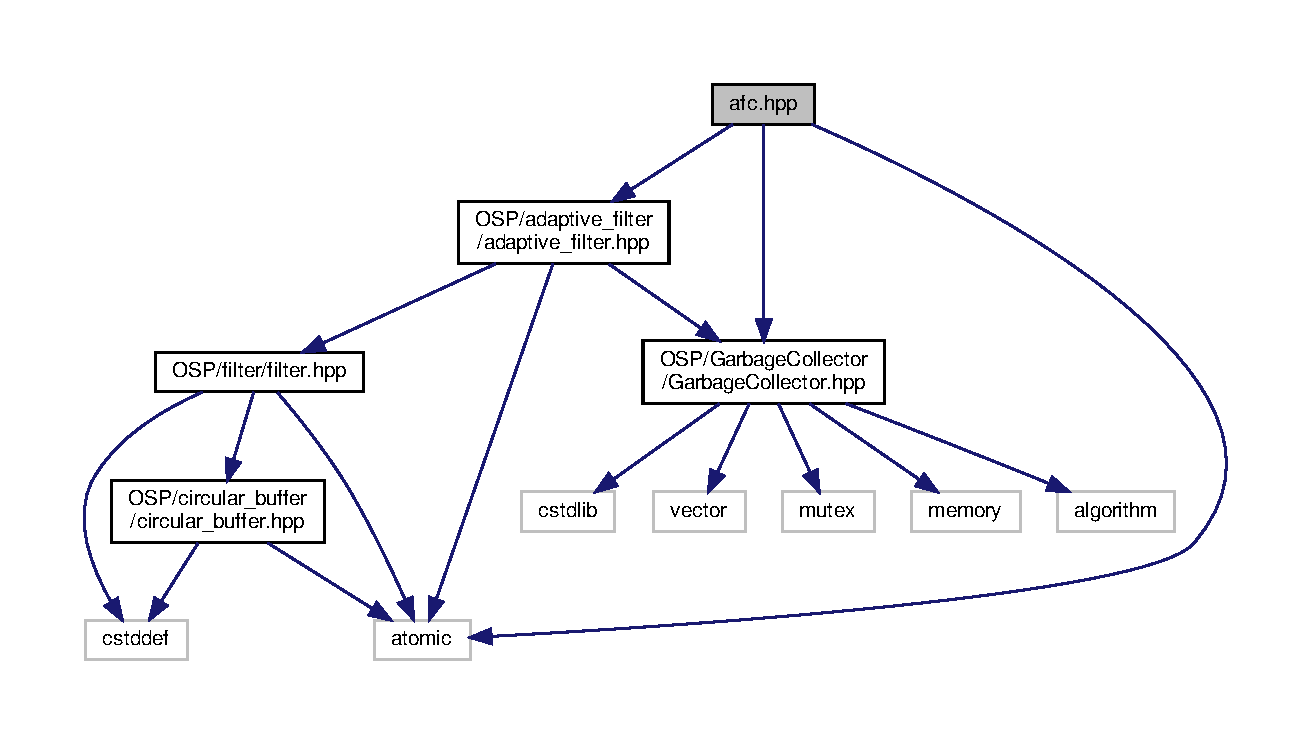
\includegraphics[width=350pt]{afc_8hpp__incl}
\end{center}
\end{figure}
This graph shows which files directly or indirectly include this file\+:\nopagebreak
\begin{figure}[H]
\begin{center}
\leavevmode
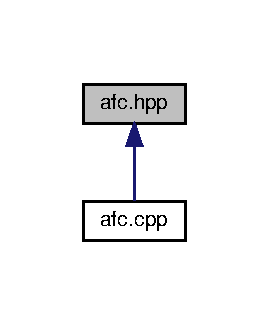
\includegraphics[width=129pt]{afc_8hpp__dep__incl}
\end{center}
\end{figure}
\subsection*{Classes}
\begin{DoxyCompactItemize}
\item 
class \hyperlink{classafc}{afc}
\begin{DoxyCompactList}\small\item\em Adaptive Feedback Cancellation (A\+FC) Class. \end{DoxyCompactList}\end{DoxyCompactItemize}
\subsection*{Macros}
\begin{DoxyCompactItemize}
\item 
\mbox{\Hypertarget{afc_8hpp_a9569aa3e973c63041f301d34fe8c52ec}\label{afc_8hpp_a9569aa3e973c63041f301d34fe8c52ec}} 
\#define {\bfseries M\+A\+X\+\_\+\+D\+E\+L\+A\+Y\+\_\+\+L\+EN}~256
\end{DoxyCompactItemize}


\subsection{Detailed Description}
\begin{DoxyAuthor}{Author}
Open Speech Platform (O\+SP) Team, U\+C\+SD 
\end{DoxyAuthor}
\begin{DoxyCopyright}{Copyright}
Copyright (C) 2020 Regents of the University of California Redistribution and use in source and binary forms, with or without modification, are permitted provided that the following conditions are met\+: \begin{DoxyVerb}1. Redistributions of source code must retain the above copyright notice, this list of conditions and the
following disclaimer.

2. Redistributions in binary form must reproduce the above copyright notice, this list of conditions and the
following disclaimer in the documentation and/or other materials provided with the distribution.
\end{DoxyVerb}

\end{DoxyCopyright}
T\+H\+IS S\+O\+F\+T\+W\+A\+RE IS P\+R\+O\+V\+I\+D\+ED BY T\+HE C\+O\+P\+Y\+R\+I\+G\+HT H\+O\+L\+D\+E\+RS A\+ND C\+O\+N\+T\+R\+I\+B\+U\+T\+O\+RS \char`\"{}\+A\+S I\+S\char`\"{} A\+ND A\+NY E\+X\+P\+R\+E\+SS OR I\+M\+P\+L\+I\+ED W\+A\+R\+R\+A\+N\+T\+I\+ES, I\+N\+C\+L\+U\+D\+I\+NG, B\+UT N\+OT L\+I\+M\+I\+T\+ED TO, T\+HE I\+M\+P\+L\+I\+ED W\+A\+R\+R\+A\+N\+T\+I\+ES OF M\+E\+R\+C\+H\+A\+N\+T\+A\+B\+I\+L\+I\+TY A\+ND F\+I\+T\+N\+E\+SS F\+OR A P\+A\+R\+T\+I\+C\+U\+L\+AR P\+U\+R\+P\+O\+SE A\+RE D\+I\+S\+C\+L\+A\+I\+M\+ED. IN NO E\+V\+E\+NT S\+H\+A\+LL T\+HE C\+O\+P\+Y\+R\+I\+G\+HT H\+O\+L\+D\+ER OR C\+O\+N\+T\+R\+I\+B\+U\+T\+O\+RS BE L\+I\+A\+B\+LE F\+OR A\+NY D\+I\+R\+E\+CT, I\+N\+D\+I\+R\+E\+CT, I\+N\+C\+I\+D\+E\+N\+T\+AL, S\+P\+E\+C\+I\+AL, E\+X\+E\+M\+P\+L\+A\+RY, OR C\+O\+N\+S\+E\+Q\+U\+E\+N\+T\+I\+AL D\+A\+M\+A\+G\+ES (I\+N\+C\+L\+U\+D\+I\+NG, B\+UT N\+OT L\+I\+M\+I\+T\+ED TO, P\+R\+O\+C\+U\+R\+E\+M\+E\+NT OF S\+U\+B\+S\+T\+I\+T\+U\+TE G\+O\+O\+DS OR S\+E\+R\+V\+I\+C\+ES; L\+O\+SS OF U\+SE, D\+A\+TA, OR P\+R\+O\+F\+I\+TS; OR B\+U\+S\+I\+N\+E\+SS I\+N\+T\+E\+R\+R\+U\+P\+T\+I\+ON) H\+O\+W\+E\+V\+ER C\+A\+U\+S\+ED A\+ND ON A\+NY T\+H\+E\+O\+RY OF L\+I\+A\+B\+I\+L\+I\+TY, W\+H\+E\+T\+H\+ER IN C\+O\+N\+T\+R\+A\+CT, S\+T\+R\+I\+CT L\+I\+A\+B\+I\+L\+I\+TY, OR T\+O\+RT (I\+N\+C\+L\+U\+D\+I\+NG N\+E\+G\+L\+I\+G\+E\+N\+CE OR O\+T\+H\+E\+R\+W\+I\+SE) A\+R\+I\+S\+I\+NG IN A\+NY W\+AY O\+UT OF T\+HE U\+SE OF T\+H\+IS S\+O\+F\+T\+W\+A\+RE, E\+V\+EN IF A\+D\+V\+I\+S\+ED OF T\+HE P\+O\+S\+S\+I\+B\+I\+L\+I\+TY OF S\+U\+CH D\+A\+M\+A\+GE. 
\hypertarget{afc__init__filter_8h}{}\section{afc\+\_\+init\+\_\+filter.\+h File Reference}
\label{afc__init__filter_8h}\index{afc\+\_\+init\+\_\+filter.\+h@{afc\+\_\+init\+\_\+filter.\+h}}
\subsection*{Macros}
\begin{DoxyCompactItemize}
\item 
\mbox{\Hypertarget{afc__init__filter_8h_aaf8d9fd6ebbddf225e77fdef778721cd}\label{afc__init__filter_8h_aaf8d9fd6ebbddf225e77fdef778721cd}} 
\#define {\bfseries A\+F\+C\+\_\+\+I\+N\+I\+T\+\_\+\+F\+I\+L\+T\+E\+R\+\_\+\+S\+I\+ZE}~160
\end{DoxyCompactItemize}
\subsection*{Variables}
\begin{DoxyCompactItemize}
\item 
\mbox{\Hypertarget{afc__init__filter_8h_a7ff24198feba948cfc065c3c74647719}\label{afc__init__filter_8h_a7ff24198feba948cfc065c3c74647719}} 
float {\bfseries afc\+\_\+init\+\_\+filter} \mbox{[}A\+F\+C\+\_\+\+I\+N\+I\+T\+\_\+\+F\+I\+L\+T\+E\+R\+\_\+\+S\+I\+ZE\mbox{]}
\end{DoxyCompactItemize}


\subsection{Detailed Description}
\begin{DoxyAuthor}{Author}
Open Speech Platform (O\+SP) Team, U\+C\+SD 
\end{DoxyAuthor}
\begin{DoxyCopyright}{Copyright}
Copyright (C) 2020 Regents of the University of California Redistribution and use in source and binary forms, with or without modification, are permitted provided that the following conditions are met\+: \begin{DoxyVerb}1. Redistributions of source code must retain the above copyright notice, this list of conditions and the
following disclaimer.

2. Redistributions in binary form must reproduce the above copyright notice, this list of conditions and the
following disclaimer in the documentation and/or other materials provided with the distribution.
\end{DoxyVerb}

\end{DoxyCopyright}
T\+H\+IS S\+O\+F\+T\+W\+A\+RE IS P\+R\+O\+V\+I\+D\+ED BY T\+HE C\+O\+P\+Y\+R\+I\+G\+HT H\+O\+L\+D\+E\+RS A\+ND C\+O\+N\+T\+R\+I\+B\+U\+T\+O\+RS \char`\"{}\+A\+S I\+S\char`\"{} A\+ND A\+NY E\+X\+P\+R\+E\+SS OR I\+M\+P\+L\+I\+ED W\+A\+R\+R\+A\+N\+T\+I\+ES, I\+N\+C\+L\+U\+D\+I\+NG, B\+UT N\+OT L\+I\+M\+I\+T\+ED TO, T\+HE I\+M\+P\+L\+I\+ED W\+A\+R\+R\+A\+N\+T\+I\+ES OF M\+E\+R\+C\+H\+A\+N\+T\+A\+B\+I\+L\+I\+TY A\+ND F\+I\+T\+N\+E\+SS F\+OR A P\+A\+R\+T\+I\+C\+U\+L\+AR P\+U\+R\+P\+O\+SE A\+RE D\+I\+S\+C\+L\+A\+I\+M\+ED. IN NO E\+V\+E\+NT S\+H\+A\+LL T\+HE C\+O\+P\+Y\+R\+I\+G\+HT H\+O\+L\+D\+ER OR C\+O\+N\+T\+R\+I\+B\+U\+T\+O\+RS BE L\+I\+A\+B\+LE F\+OR A\+NY D\+I\+R\+E\+CT, I\+N\+D\+I\+R\+E\+CT, I\+N\+C\+I\+D\+E\+N\+T\+AL, S\+P\+E\+C\+I\+AL, E\+X\+E\+M\+P\+L\+A\+RY, OR C\+O\+N\+S\+E\+Q\+U\+E\+N\+T\+I\+AL D\+A\+M\+A\+G\+ES (I\+N\+C\+L\+U\+D\+I\+NG, B\+UT N\+OT L\+I\+M\+I\+T\+ED TO, P\+R\+O\+C\+U\+R\+E\+M\+E\+NT OF S\+U\+B\+S\+T\+I\+T\+U\+TE G\+O\+O\+DS OR S\+E\+R\+V\+I\+C\+ES; L\+O\+SS OF U\+SE, D\+A\+TA, OR P\+R\+O\+F\+I\+TS; OR B\+U\+S\+I\+N\+E\+SS I\+N\+T\+E\+R\+R\+U\+P\+T\+I\+ON) H\+O\+W\+E\+V\+ER C\+A\+U\+S\+ED A\+ND ON A\+NY T\+H\+E\+O\+RY OF L\+I\+A\+B\+I\+L\+I\+TY, W\+H\+E\+T\+H\+ER IN C\+O\+N\+T\+R\+A\+CT, S\+T\+R\+I\+CT L\+I\+A\+B\+I\+L\+I\+TY, OR T\+O\+RT (I\+N\+C\+L\+U\+D\+I\+NG N\+E\+G\+L\+I\+G\+E\+N\+CE OR O\+T\+H\+E\+R\+W\+I\+SE) A\+R\+I\+S\+I\+NG IN A\+NY W\+AY O\+UT OF T\+HE U\+SE OF T\+H\+IS S\+O\+F\+T\+W\+A\+RE, E\+V\+EN IF A\+D\+V\+I\+S\+ED OF T\+HE P\+O\+S\+S\+I\+B\+I\+L\+I\+TY OF S\+U\+CH D\+A\+M\+A\+GE. 
\hypertarget{array__file_8cpp}{}\section{array\+\_\+file.\+cpp File Reference}
\label{array__file_8cpp}\index{array\+\_\+file.\+cpp@{array\+\_\+file.\+cpp}}
{\ttfamily \#include $<$stdlib.\+h$>$}\newline
{\ttfamily \#include $<$string$>$}\newline
{\ttfamily \#include $<$fstream$>$}\newline
{\ttfamily \#include $<$O\+S\+P/array\+\_\+file/array\+\_\+file.\+hpp$>$}\newline
Include dependency graph for array\+\_\+file.\+cpp\+:\nopagebreak
\begin{figure}[H]
\begin{center}
\leavevmode
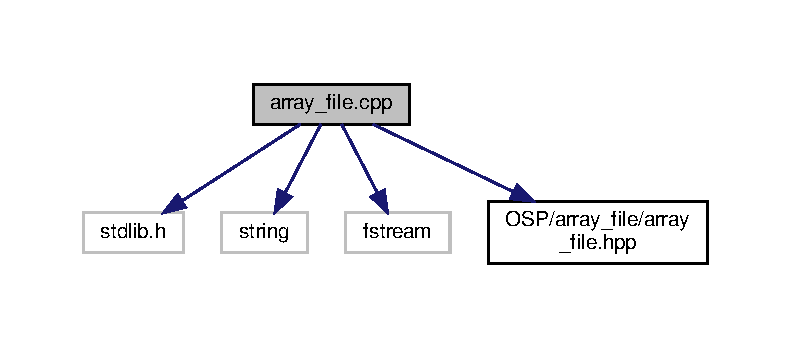
\includegraphics[width=350pt]{array__file_8cpp__incl}
\end{center}
\end{figure}


\subsection{Detailed Description}
\begin{DoxyAuthor}{Author}
Open Speech Platform (O\+SP) Team, U\+C\+SD 
\end{DoxyAuthor}
\begin{DoxyCopyright}{Copyright}
Copyright (C) 2020 Regents of the University of California Redistribution and use in source and binary forms, with or without modification, are permitted provided that the following conditions are met\+: \begin{DoxyVerb}1. Redistributions of source code must retain the above copyright notice, this list of conditions and the
following disclaimer.

2. Redistributions in binary form must reproduce the above copyright notice, this list of conditions and the
following disclaimer in the documentation and/or other materials provided with the distribution.
\end{DoxyVerb}

\end{DoxyCopyright}
T\+H\+IS S\+O\+F\+T\+W\+A\+RE IS P\+R\+O\+V\+I\+D\+ED BY T\+HE C\+O\+P\+Y\+R\+I\+G\+HT H\+O\+L\+D\+E\+RS A\+ND C\+O\+N\+T\+R\+I\+B\+U\+T\+O\+RS \char`\"{}\+A\+S I\+S\char`\"{} A\+ND A\+NY E\+X\+P\+R\+E\+SS OR I\+M\+P\+L\+I\+ED W\+A\+R\+R\+A\+N\+T\+I\+ES, I\+N\+C\+L\+U\+D\+I\+NG, B\+UT N\+OT L\+I\+M\+I\+T\+ED TO, T\+HE I\+M\+P\+L\+I\+ED W\+A\+R\+R\+A\+N\+T\+I\+ES OF M\+E\+R\+C\+H\+A\+N\+T\+A\+B\+I\+L\+I\+TY A\+ND F\+I\+T\+N\+E\+SS F\+OR A P\+A\+R\+T\+I\+C\+U\+L\+AR P\+U\+R\+P\+O\+SE A\+RE D\+I\+S\+C\+L\+A\+I\+M\+ED. IN NO E\+V\+E\+NT S\+H\+A\+LL T\+HE C\+O\+P\+Y\+R\+I\+G\+HT H\+O\+L\+D\+ER OR C\+O\+N\+T\+R\+I\+B\+U\+T\+O\+RS BE L\+I\+A\+B\+LE F\+OR A\+NY D\+I\+R\+E\+CT, I\+N\+D\+I\+R\+E\+CT, I\+N\+C\+I\+D\+E\+N\+T\+AL, S\+P\+E\+C\+I\+AL, E\+X\+E\+M\+P\+L\+A\+RY, OR C\+O\+N\+S\+E\+Q\+U\+E\+N\+T\+I\+AL D\+A\+M\+A\+G\+ES (I\+N\+C\+L\+U\+D\+I\+NG, B\+UT N\+OT L\+I\+M\+I\+T\+ED TO, P\+R\+O\+C\+U\+R\+E\+M\+E\+NT OF S\+U\+B\+S\+T\+I\+T\+U\+TE G\+O\+O\+DS OR S\+E\+R\+V\+I\+C\+ES; L\+O\+SS OF U\+SE, D\+A\+TA, OR P\+R\+O\+F\+I\+TS; OR B\+U\+S\+I\+N\+E\+SS I\+N\+T\+E\+R\+R\+U\+P\+T\+I\+ON) H\+O\+W\+E\+V\+ER C\+A\+U\+S\+ED A\+ND ON A\+NY T\+H\+E\+O\+RY OF L\+I\+A\+B\+I\+L\+I\+TY, W\+H\+E\+T\+H\+ER IN C\+O\+N\+T\+R\+A\+CT, S\+T\+R\+I\+CT L\+I\+A\+B\+I\+L\+I\+TY, OR T\+O\+RT (I\+N\+C\+L\+U\+D\+I\+NG N\+E\+G\+L\+I\+G\+E\+N\+CE OR O\+T\+H\+E\+R\+W\+I\+SE) A\+R\+I\+S\+I\+NG IN A\+NY W\+AY O\+UT OF T\+HE U\+SE OF T\+H\+IS S\+O\+F\+T\+W\+A\+RE, E\+V\+EN IF A\+D\+V\+I\+S\+ED OF T\+HE P\+O\+S\+S\+I\+B\+I\+L\+I\+TY OF S\+U\+CH D\+A\+M\+A\+GE. 
\hypertarget{array__file_8hpp}{}\section{array\+\_\+file.\+hpp File Reference}
\label{array__file_8hpp}\index{array\+\_\+file.\+hpp@{array\+\_\+file.\+hpp}}
This graph shows which files directly or indirectly include this file\+:\nopagebreak
\begin{figure}[H]
\begin{center}
\leavevmode
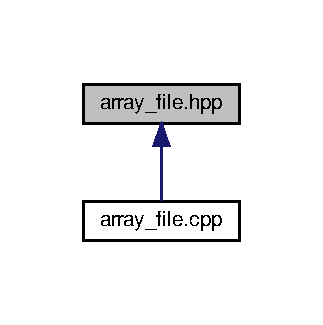
\includegraphics[width=155pt]{array__file_8hpp__dep__incl}
\end{center}
\end{figure}
\subsection*{Classes}
\begin{DoxyCompactItemize}
\item 
class \hyperlink{classarray__file}{array\+\_\+file}
\begin{DoxyCompactList}\small\item\em Array File Class. \end{DoxyCompactList}\end{DoxyCompactItemize}


\subsection{Detailed Description}
\begin{DoxyAuthor}{Author}
Open Speech Platform (O\+SP) Team, U\+C\+SD 
\end{DoxyAuthor}
\begin{DoxyCopyright}{Copyright}
Copyright (C) 2020 Regents of the University of California Redistribution and use in source and binary forms, with or without modification, are permitted provided that the following conditions are met\+: \begin{DoxyVerb}1. Redistributions of source code must retain the above copyright notice, this list of conditions and the
following disclaimer.

2. Redistributions in binary form must reproduce the above copyright notice, this list of conditions and the
following disclaimer in the documentation and/or other materials provided with the distribution.
\end{DoxyVerb}

\end{DoxyCopyright}
T\+H\+IS S\+O\+F\+T\+W\+A\+RE IS P\+R\+O\+V\+I\+D\+ED BY T\+HE C\+O\+P\+Y\+R\+I\+G\+HT H\+O\+L\+D\+E\+RS A\+ND C\+O\+N\+T\+R\+I\+B\+U\+T\+O\+RS \char`\"{}\+A\+S I\+S\char`\"{} A\+ND A\+NY E\+X\+P\+R\+E\+SS OR I\+M\+P\+L\+I\+ED W\+A\+R\+R\+A\+N\+T\+I\+ES, I\+N\+C\+L\+U\+D\+I\+NG, B\+UT N\+OT L\+I\+M\+I\+T\+ED TO, T\+HE I\+M\+P\+L\+I\+ED W\+A\+R\+R\+A\+N\+T\+I\+ES OF M\+E\+R\+C\+H\+A\+N\+T\+A\+B\+I\+L\+I\+TY A\+ND F\+I\+T\+N\+E\+SS F\+OR A P\+A\+R\+T\+I\+C\+U\+L\+AR P\+U\+R\+P\+O\+SE A\+RE D\+I\+S\+C\+L\+A\+I\+M\+ED. IN NO E\+V\+E\+NT S\+H\+A\+LL T\+HE C\+O\+P\+Y\+R\+I\+G\+HT H\+O\+L\+D\+ER OR C\+O\+N\+T\+R\+I\+B\+U\+T\+O\+RS BE L\+I\+A\+B\+LE F\+OR A\+NY D\+I\+R\+E\+CT, I\+N\+D\+I\+R\+E\+CT, I\+N\+C\+I\+D\+E\+N\+T\+AL, S\+P\+E\+C\+I\+AL, E\+X\+E\+M\+P\+L\+A\+RY, OR C\+O\+N\+S\+E\+Q\+U\+E\+N\+T\+I\+AL D\+A\+M\+A\+G\+ES (I\+N\+C\+L\+U\+D\+I\+NG, B\+UT N\+OT L\+I\+M\+I\+T\+ED TO, P\+R\+O\+C\+U\+R\+E\+M\+E\+NT OF S\+U\+B\+S\+T\+I\+T\+U\+TE G\+O\+O\+DS OR S\+E\+R\+V\+I\+C\+ES; L\+O\+SS OF U\+SE, D\+A\+TA, OR P\+R\+O\+F\+I\+TS; OR B\+U\+S\+I\+N\+E\+SS I\+N\+T\+E\+R\+R\+U\+P\+T\+I\+ON) H\+O\+W\+E\+V\+ER C\+A\+U\+S\+ED A\+ND ON A\+NY T\+H\+E\+O\+RY OF L\+I\+A\+B\+I\+L\+I\+TY, W\+H\+E\+T\+H\+ER IN C\+O\+N\+T\+R\+A\+CT, S\+T\+R\+I\+CT L\+I\+A\+B\+I\+L\+I\+TY, OR T\+O\+RT (I\+N\+C\+L\+U\+D\+I\+NG N\+E\+G\+L\+I\+G\+E\+N\+CE OR O\+T\+H\+E\+R\+W\+I\+SE) A\+R\+I\+S\+I\+NG IN A\+NY W\+AY O\+UT OF T\+HE U\+SE OF T\+H\+IS S\+O\+F\+T\+W\+A\+RE, E\+V\+EN IF A\+D\+V\+I\+S\+ED OF T\+HE P\+O\+S\+S\+I\+B\+I\+L\+I\+TY OF S\+U\+CH D\+A\+M\+A\+GE. 
\hypertarget{array__utilities_8cpp}{}\section{array\+\_\+utilities.\+cpp File Reference}
\label{array__utilities_8cpp}\index{array\+\_\+utilities.\+cpp@{array\+\_\+utilities.\+cpp}}
{\ttfamily \#include $<$cstdio$>$}\newline
{\ttfamily \#include $<$O\+S\+P/array\+\_\+utilities/array\+\_\+utilities.\+hpp$>$}\newline
Include dependency graph for array\+\_\+utilities.\+cpp\+:\nopagebreak
\begin{figure}[H]
\begin{center}
\leavevmode
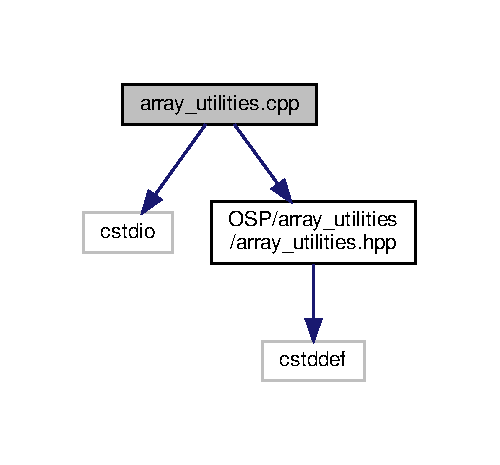
\includegraphics[width=240pt]{array__utilities_8cpp__incl}
\end{center}
\end{figure}
\subsection*{Functions}
\begin{DoxyCompactItemize}
\item 
void \hyperlink{array__utilities_8cpp_a671b885d4bc80890d5db79251c179cc6}{array\+\_\+flip} (float $\ast$arr, size\+\_\+t len)
\begin{DoxyCompactList}\small\item\em Function to reverse an array. \end{DoxyCompactList}\item 
float \hyperlink{array__utilities_8cpp_a951da7a6e40691865c6b669e65235848}{array\+\_\+sum} (const float $\ast$arr, size\+\_\+t len)
\begin{DoxyCompactList}\small\item\em Function to calculate the sum of an array. \end{DoxyCompactList}\item 
float \hyperlink{array__utilities_8cpp_a553c08dad0548039a851968d25767881}{array\+\_\+dot\+\_\+product} (const float $\ast$in1, const float $\ast$in2, size\+\_\+t len)
\begin{DoxyCompactList}\small\item\em Function to calculate the dot-\/product of two 1-\/D vectors/arrays. \end{DoxyCompactList}\item 
void \hyperlink{array__utilities_8cpp_ac5e150940a31a2aace5bc977dfed62e7}{array\+\_\+right\+\_\+shift} (float $\ast$arr, size\+\_\+t len)
\begin{DoxyCompactList}\small\item\em Function to right shift an array by one place. Left most value will be replaced by zero. \end{DoxyCompactList}\item 
void \hyperlink{array__utilities_8cpp_ae9c0f53e57eba1f9b68b3b98035c7104}{array\+\_\+multiply\+\_\+const} (float $\ast$arr, float constant, size\+\_\+t len)
\begin{DoxyCompactList}\small\item\em Function to multiply each element of an array by a scalar constant. \end{DoxyCompactList}\item 
void \hyperlink{array__utilities_8cpp_ac5021e5ce6e8fbcdefd4ec345304363e}{array\+\_\+add\+\_\+const} (float $\ast$arr, float constant, size\+\_\+t len)
\begin{DoxyCompactList}\small\item\em Function to add a scalar constant to each element of an array. \end{DoxyCompactList}\item 
void \hyperlink{array__utilities_8cpp_aeb83126cafbf7b72e9c4229b630f93f7}{array\+\_\+add\+\_\+array} (float $\ast$in1, const float $\ast$in2, size\+\_\+t len)
\begin{DoxyCompactList}\small\item\em Function to do element wise addition of two arrays. \end{DoxyCompactList}\item 
void \hyperlink{array__utilities_8cpp_a16c4485ad0fc4addbd8e4966b6c2dd34}{array\+\_\+subtract\+\_\+array} (float $\ast$in1, const float $\ast$in2, size\+\_\+t len)
\begin{DoxyCompactList}\small\item\em Function to do element wise subtraction of two arrays. \end{DoxyCompactList}\item 
void \hyperlink{array__utilities_8cpp_a5d18621319de15256d97586e9be833b5}{array\+\_\+element\+\_\+multiply\+\_\+array} (float $\ast$in1, const float $\ast$in2, size\+\_\+t len)
\begin{DoxyCompactList}\small\item\em Function to do element wise multiplication of two arrays. \end{DoxyCompactList}\item 
void \hyperlink{array__utilities_8cpp_ace8a12bb47149c5215616caf9dd5d594}{array\+\_\+element\+\_\+divide\+\_\+array} (float $\ast$in1, const float $\ast$in2, size\+\_\+t len)
\begin{DoxyCompactList}\small\item\em Function to do element wise division of two arrays. \end{DoxyCompactList}\item 
float \hyperlink{array__utilities_8cpp_a9a766be2ca62f99e043583cd6ae183fc}{array\+\_\+min} (const float $\ast$arr, size\+\_\+t len)
\begin{DoxyCompactList}\small\item\em Function to return the minimum of the elements of an array. \end{DoxyCompactList}\item 
float \hyperlink{array__utilities_8cpp_abd95915e71cdf97c66dd2092aed740df}{array\+\_\+mean} (float $\ast$arr, size\+\_\+t len)
\begin{DoxyCompactList}\small\item\em Function to calculate the mean of the elements of an array. \end{DoxyCompactList}\item 
void \hyperlink{array__utilities_8cpp_a41f17b8ac6c9f77c6bc16231a35b0304}{array\+\_\+square} (const float $\ast$in, float $\ast$out, size\+\_\+t len)
\begin{DoxyCompactList}\small\item\em Function to populate the output array with square of the elements of an input array. \end{DoxyCompactList}\item 
float \hyperlink{array__utilities_8cpp_a7adedf9123b714557d3d35ed500d82b9}{array\+\_\+mean\+\_\+square} (const float $\ast$arr, size\+\_\+t len)
\begin{DoxyCompactList}\small\item\em Function to calculate the mean square of the elements of an array. \end{DoxyCompactList}\item 
void \hyperlink{array__utilities_8cpp_ad1f8261eef0b72711c198bdc73fb934d}{array\+\_\+print} (const char $\ast$str, float $\ast$arr, size\+\_\+t len)
\begin{DoxyCompactList}\small\item\em Function to print an array for debugging. \end{DoxyCompactList}\end{DoxyCompactItemize}


\subsection{Detailed Description}
\begin{DoxyAuthor}{Author}
Open Speech Platform (O\+SP) Team, U\+C\+SD 
\end{DoxyAuthor}
\begin{DoxyCopyright}{Copyright}
Copyright (C) 2020 Regents of the University of California Redistribution and use in source and binary forms, with or without modification, are permitted provided that the following conditions are met\+: \begin{DoxyVerb}1. Redistributions of source code must retain the above copyright notice, this list of conditions and the
following disclaimer.

2. Redistributions in binary form must reproduce the above copyright notice, this list of conditions and the
following disclaimer in the documentation and/or other materials provided with the distribution.
\end{DoxyVerb}

\end{DoxyCopyright}
T\+H\+IS S\+O\+F\+T\+W\+A\+RE IS P\+R\+O\+V\+I\+D\+ED BY T\+HE C\+O\+P\+Y\+R\+I\+G\+HT H\+O\+L\+D\+E\+RS A\+ND C\+O\+N\+T\+R\+I\+B\+U\+T\+O\+RS \char`\"{}\+A\+S I\+S\char`\"{} A\+ND A\+NY E\+X\+P\+R\+E\+SS OR I\+M\+P\+L\+I\+ED W\+A\+R\+R\+A\+N\+T\+I\+ES, I\+N\+C\+L\+U\+D\+I\+NG, B\+UT N\+OT L\+I\+M\+I\+T\+ED TO, T\+HE I\+M\+P\+L\+I\+ED W\+A\+R\+R\+A\+N\+T\+I\+ES OF M\+E\+R\+C\+H\+A\+N\+T\+A\+B\+I\+L\+I\+TY A\+ND F\+I\+T\+N\+E\+SS F\+OR A P\+A\+R\+T\+I\+C\+U\+L\+AR P\+U\+R\+P\+O\+SE A\+RE D\+I\+S\+C\+L\+A\+I\+M\+ED. IN NO E\+V\+E\+NT S\+H\+A\+LL T\+HE C\+O\+P\+Y\+R\+I\+G\+HT H\+O\+L\+D\+ER OR C\+O\+N\+T\+R\+I\+B\+U\+T\+O\+RS BE L\+I\+A\+B\+LE F\+OR A\+NY D\+I\+R\+E\+CT, I\+N\+D\+I\+R\+E\+CT, I\+N\+C\+I\+D\+E\+N\+T\+AL, S\+P\+E\+C\+I\+AL, E\+X\+E\+M\+P\+L\+A\+RY, OR C\+O\+N\+S\+E\+Q\+U\+E\+N\+T\+I\+AL D\+A\+M\+A\+G\+ES (I\+N\+C\+L\+U\+D\+I\+NG, B\+UT N\+OT L\+I\+M\+I\+T\+ED TO, P\+R\+O\+C\+U\+R\+E\+M\+E\+NT OF S\+U\+B\+S\+T\+I\+T\+U\+TE G\+O\+O\+DS OR S\+E\+R\+V\+I\+C\+ES; L\+O\+SS OF U\+SE, D\+A\+TA, OR P\+R\+O\+F\+I\+TS; OR B\+U\+S\+I\+N\+E\+SS I\+N\+T\+E\+R\+R\+U\+P\+T\+I\+ON) H\+O\+W\+E\+V\+ER C\+A\+U\+S\+ED A\+ND ON A\+NY T\+H\+E\+O\+RY OF L\+I\+A\+B\+I\+L\+I\+TY, W\+H\+E\+T\+H\+ER IN C\+O\+N\+T\+R\+A\+CT, S\+T\+R\+I\+CT L\+I\+A\+B\+I\+L\+I\+TY, OR T\+O\+RT (I\+N\+C\+L\+U\+D\+I\+NG N\+E\+G\+L\+I\+G\+E\+N\+CE OR O\+T\+H\+E\+R\+W\+I\+SE) A\+R\+I\+S\+I\+NG IN A\+NY W\+AY O\+UT OF T\+HE U\+SE OF T\+H\+IS S\+O\+F\+T\+W\+A\+RE, E\+V\+EN IF A\+D\+V\+I\+S\+ED OF T\+HE P\+O\+S\+S\+I\+B\+I\+L\+I\+TY OF S\+U\+CH D\+A\+M\+A\+GE. 

\subsection{Function Documentation}
\mbox{\Hypertarget{array__utilities_8cpp_aeb83126cafbf7b72e9c4229b630f93f7}\label{array__utilities_8cpp_aeb83126cafbf7b72e9c4229b630f93f7}} 
\index{array\+\_\+utilities.\+cpp@{array\+\_\+utilities.\+cpp}!array\+\_\+add\+\_\+array@{array\+\_\+add\+\_\+array}}
\index{array\+\_\+add\+\_\+array@{array\+\_\+add\+\_\+array}!array\+\_\+utilities.\+cpp@{array\+\_\+utilities.\+cpp}}
\subsubsection{\texorpdfstring{array\+\_\+add\+\_\+array()}{array\_add\_array()}}
{\footnotesize\ttfamily void array\+\_\+add\+\_\+array (\begin{DoxyParamCaption}\item[{float $\ast$}]{in1,  }\item[{const float $\ast$}]{in2,  }\item[{size\+\_\+t}]{len }\end{DoxyParamCaption})}



Function to do element wise addition of two arrays. 


\begin{DoxyParams}{Parameters}
{\em in1} & Pointer to the first array \\
\hline
{\em in2} & Pointer to the second array \\
\hline
{\em len} & Length of the arrays \\
\hline
\end{DoxyParams}
\begin{DoxyWarning}{Warning}
Assumes both the arrays are of same length and takes only one length parameter 
\end{DoxyWarning}


Definition at line 105 of file array\+\_\+utilities.\+cpp.

\mbox{\Hypertarget{array__utilities_8cpp_ac5021e5ce6e8fbcdefd4ec345304363e}\label{array__utilities_8cpp_ac5021e5ce6e8fbcdefd4ec345304363e}} 
\index{array\+\_\+utilities.\+cpp@{array\+\_\+utilities.\+cpp}!array\+\_\+add\+\_\+const@{array\+\_\+add\+\_\+const}}
\index{array\+\_\+add\+\_\+const@{array\+\_\+add\+\_\+const}!array\+\_\+utilities.\+cpp@{array\+\_\+utilities.\+cpp}}
\subsubsection{\texorpdfstring{array\+\_\+add\+\_\+const()}{array\_add\_const()}}
{\footnotesize\ttfamily void array\+\_\+add\+\_\+const (\begin{DoxyParamCaption}\item[{float $\ast$}]{arr,  }\item[{float}]{constant,  }\item[{size\+\_\+t}]{len }\end{DoxyParamCaption})}



Function to add a scalar constant to each element of an array. 


\begin{DoxyParams}{Parameters}
{\em arr} & Pointer to the array \\
\hline
{\em constant} & The constant scalar adder \\
\hline
{\em len} & Length of the array \\
\hline
\end{DoxyParams}


Definition at line 96 of file array\+\_\+utilities.\+cpp.

\mbox{\Hypertarget{array__utilities_8cpp_a553c08dad0548039a851968d25767881}\label{array__utilities_8cpp_a553c08dad0548039a851968d25767881}} 
\index{array\+\_\+utilities.\+cpp@{array\+\_\+utilities.\+cpp}!array\+\_\+dot\+\_\+product@{array\+\_\+dot\+\_\+product}}
\index{array\+\_\+dot\+\_\+product@{array\+\_\+dot\+\_\+product}!array\+\_\+utilities.\+cpp@{array\+\_\+utilities.\+cpp}}
\subsubsection{\texorpdfstring{array\+\_\+dot\+\_\+product()}{array\_dot\_product()}}
{\footnotesize\ttfamily float array\+\_\+dot\+\_\+product (\begin{DoxyParamCaption}\item[{const float $\ast$}]{in1,  }\item[{const float $\ast$}]{in2,  }\item[{size\+\_\+t}]{len }\end{DoxyParamCaption})}



Function to calculate the dot-\/product of two 1-\/D vectors/arrays. 


\begin{DoxyParams}{Parameters}
{\em in1} & Pointer to the first vector \\
\hline
{\em in2} & Pointer to the second vector \\
\hline
{\em len} & Length of the vectors \\
\hline
\end{DoxyParams}
\begin{DoxyReturn}{Returns}
Dot product (inner product) of the two vectors 
\end{DoxyReturn}
\begin{DoxyWarning}{Warning}
Assumes both the vectors are of same length and takes only one length parameter 
\end{DoxyWarning}


Definition at line 67 of file array\+\_\+utilities.\+cpp.

\mbox{\Hypertarget{array__utilities_8cpp_ace8a12bb47149c5215616caf9dd5d594}\label{array__utilities_8cpp_ace8a12bb47149c5215616caf9dd5d594}} 
\index{array\+\_\+utilities.\+cpp@{array\+\_\+utilities.\+cpp}!array\+\_\+element\+\_\+divide\+\_\+array@{array\+\_\+element\+\_\+divide\+\_\+array}}
\index{array\+\_\+element\+\_\+divide\+\_\+array@{array\+\_\+element\+\_\+divide\+\_\+array}!array\+\_\+utilities.\+cpp@{array\+\_\+utilities.\+cpp}}
\subsubsection{\texorpdfstring{array\+\_\+element\+\_\+divide\+\_\+array()}{array\_element\_divide\_array()}}
{\footnotesize\ttfamily void array\+\_\+element\+\_\+divide\+\_\+array (\begin{DoxyParamCaption}\item[{float $\ast$}]{in1,  }\item[{const float $\ast$}]{in2,  }\item[{size\+\_\+t}]{len }\end{DoxyParamCaption})}



Function to do element wise division of two arrays. 


\begin{DoxyParams}{Parameters}
{\em in1} & Pointer to the first array \\
\hline
{\em in2} & Pointer to the second array \\
\hline
{\em len} & Length of the arrays \\
\hline
\end{DoxyParams}
\begin{DoxyWarning}{Warning}
Assumes both the arrays are of same length and takes only one length parameter 
\end{DoxyWarning}


Definition at line 132 of file array\+\_\+utilities.\+cpp.

\mbox{\Hypertarget{array__utilities_8cpp_a5d18621319de15256d97586e9be833b5}\label{array__utilities_8cpp_a5d18621319de15256d97586e9be833b5}} 
\index{array\+\_\+utilities.\+cpp@{array\+\_\+utilities.\+cpp}!array\+\_\+element\+\_\+multiply\+\_\+array@{array\+\_\+element\+\_\+multiply\+\_\+array}}
\index{array\+\_\+element\+\_\+multiply\+\_\+array@{array\+\_\+element\+\_\+multiply\+\_\+array}!array\+\_\+utilities.\+cpp@{array\+\_\+utilities.\+cpp}}
\subsubsection{\texorpdfstring{array\+\_\+element\+\_\+multiply\+\_\+array()}{array\_element\_multiply\_array()}}
{\footnotesize\ttfamily void array\+\_\+element\+\_\+multiply\+\_\+array (\begin{DoxyParamCaption}\item[{float $\ast$}]{in1,  }\item[{const float $\ast$}]{in2,  }\item[{size\+\_\+t}]{len }\end{DoxyParamCaption})}



Function to do element wise multiplication of two arrays. 


\begin{DoxyParams}{Parameters}
{\em in1} & Pointer to the first array \\
\hline
{\em in2} & Pointer to the second array \\
\hline
{\em len} & Length of the arrays \\
\hline
\end{DoxyParams}
\begin{DoxyWarning}{Warning}
Assumes both the arrays are of same length and takes only one length parameter 
\end{DoxyWarning}


Definition at line 123 of file array\+\_\+utilities.\+cpp.

\mbox{\Hypertarget{array__utilities_8cpp_a671b885d4bc80890d5db79251c179cc6}\label{array__utilities_8cpp_a671b885d4bc80890d5db79251c179cc6}} 
\index{array\+\_\+utilities.\+cpp@{array\+\_\+utilities.\+cpp}!array\+\_\+flip@{array\+\_\+flip}}
\index{array\+\_\+flip@{array\+\_\+flip}!array\+\_\+utilities.\+cpp@{array\+\_\+utilities.\+cpp}}
\subsubsection{\texorpdfstring{array\+\_\+flip()}{array\_flip()}}
{\footnotesize\ttfamily void array\+\_\+flip (\begin{DoxyParamCaption}\item[{float $\ast$}]{arr,  }\item[{size\+\_\+t}]{len }\end{DoxyParamCaption})}



Function to reverse an array. 


\begin{DoxyParams}{Parameters}
{\em arr} & Pointer to the array \\
\hline
{\em len} & Length of the array \\
\hline
\end{DoxyParams}


Definition at line 31 of file array\+\_\+utilities.\+cpp.

\mbox{\Hypertarget{array__utilities_8cpp_abd95915e71cdf97c66dd2092aed740df}\label{array__utilities_8cpp_abd95915e71cdf97c66dd2092aed740df}} 
\index{array\+\_\+utilities.\+cpp@{array\+\_\+utilities.\+cpp}!array\+\_\+mean@{array\+\_\+mean}}
\index{array\+\_\+mean@{array\+\_\+mean}!array\+\_\+utilities.\+cpp@{array\+\_\+utilities.\+cpp}}
\subsubsection{\texorpdfstring{array\+\_\+mean()}{array\_mean()}}
{\footnotesize\ttfamily float array\+\_\+mean (\begin{DoxyParamCaption}\item[{float $\ast$}]{arr,  }\item[{size\+\_\+t}]{len }\end{DoxyParamCaption})}



Function to calculate the mean of the elements of an array. 


\begin{DoxyParams}{Parameters}
{\em arr} & Pointer to the array \\
\hline
{\em len} & Length of the array \\
\hline
\end{DoxyParams}
\begin{DoxyReturn}{Returns}
Mean of the array elements 
\end{DoxyReturn}


Definition at line 156 of file array\+\_\+utilities.\+cpp.

\mbox{\Hypertarget{array__utilities_8cpp_a7adedf9123b714557d3d35ed500d82b9}\label{array__utilities_8cpp_a7adedf9123b714557d3d35ed500d82b9}} 
\index{array\+\_\+utilities.\+cpp@{array\+\_\+utilities.\+cpp}!array\+\_\+mean\+\_\+square@{array\+\_\+mean\+\_\+square}}
\index{array\+\_\+mean\+\_\+square@{array\+\_\+mean\+\_\+square}!array\+\_\+utilities.\+cpp@{array\+\_\+utilities.\+cpp}}
\subsubsection{\texorpdfstring{array\+\_\+mean\+\_\+square()}{array\_mean\_square()}}
{\footnotesize\ttfamily float array\+\_\+mean\+\_\+square (\begin{DoxyParamCaption}\item[{const float $\ast$}]{arr,  }\item[{size\+\_\+t}]{len }\end{DoxyParamCaption})}



Function to calculate the mean square of the elements of an array. 


\begin{DoxyParams}{Parameters}
{\em arr} & Pointer to the array \\
\hline
{\em len} & Length of the array \\
\hline
\end{DoxyParams}
\begin{DoxyReturn}{Returns}
Mean square of the array elements 
\end{DoxyReturn}


Definition at line 172 of file array\+\_\+utilities.\+cpp.

\mbox{\Hypertarget{array__utilities_8cpp_a9a766be2ca62f99e043583cd6ae183fc}\label{array__utilities_8cpp_a9a766be2ca62f99e043583cd6ae183fc}} 
\index{array\+\_\+utilities.\+cpp@{array\+\_\+utilities.\+cpp}!array\+\_\+min@{array\+\_\+min}}
\index{array\+\_\+min@{array\+\_\+min}!array\+\_\+utilities.\+cpp@{array\+\_\+utilities.\+cpp}}
\subsubsection{\texorpdfstring{array\+\_\+min()}{array\_min()}}
{\footnotesize\ttfamily float array\+\_\+min (\begin{DoxyParamCaption}\item[{const float $\ast$}]{arr,  }\item[{size\+\_\+t}]{len }\end{DoxyParamCaption})}



Function to return the minimum of the elements of an array. 


\begin{DoxyParams}{Parameters}
{\em arr} & Pointer to the array \\
\hline
{\em len} & Length of the array \\
\hline
\end{DoxyParams}
\begin{DoxyReturn}{Returns}
Minimum of the array elements 
\end{DoxyReturn}


Definition at line 141 of file array\+\_\+utilities.\+cpp.

\mbox{\Hypertarget{array__utilities_8cpp_ae9c0f53e57eba1f9b68b3b98035c7104}\label{array__utilities_8cpp_ae9c0f53e57eba1f9b68b3b98035c7104}} 
\index{array\+\_\+utilities.\+cpp@{array\+\_\+utilities.\+cpp}!array\+\_\+multiply\+\_\+const@{array\+\_\+multiply\+\_\+const}}
\index{array\+\_\+multiply\+\_\+const@{array\+\_\+multiply\+\_\+const}!array\+\_\+utilities.\+cpp@{array\+\_\+utilities.\+cpp}}
\subsubsection{\texorpdfstring{array\+\_\+multiply\+\_\+const()}{array\_multiply\_const()}}
{\footnotesize\ttfamily void array\+\_\+multiply\+\_\+const (\begin{DoxyParamCaption}\item[{float $\ast$}]{arr,  }\item[{float}]{constant,  }\item[{size\+\_\+t}]{len }\end{DoxyParamCaption})}



Function to multiply each element of an array by a scalar constant. 


\begin{DoxyParams}{Parameters}
{\em arr} & Pointer to the array \\
\hline
{\em constant} & The constant scalar multiplier \\
\hline
{\em len} & Length of the array \\
\hline
\end{DoxyParams}


Definition at line 87 of file array\+\_\+utilities.\+cpp.

\mbox{\Hypertarget{array__utilities_8cpp_ad1f8261eef0b72711c198bdc73fb934d}\label{array__utilities_8cpp_ad1f8261eef0b72711c198bdc73fb934d}} 
\index{array\+\_\+utilities.\+cpp@{array\+\_\+utilities.\+cpp}!array\+\_\+print@{array\+\_\+print}}
\index{array\+\_\+print@{array\+\_\+print}!array\+\_\+utilities.\+cpp@{array\+\_\+utilities.\+cpp}}
\subsubsection{\texorpdfstring{array\+\_\+print()}{array\_print()}}
{\footnotesize\ttfamily void array\+\_\+print (\begin{DoxyParamCaption}\item[{const char $\ast$}]{str,  }\item[{float $\ast$}]{arr,  }\item[{size\+\_\+t}]{len }\end{DoxyParamCaption})}



Function to print an array for debugging. 


\begin{DoxyParams}{Parameters}
{\em str} & String to use for debugging \\
\hline
{\em arr} & Pointer to the array \\
\hline
{\em len} & Length of the array \\
\hline
\end{DoxyParams}


Definition at line 177 of file array\+\_\+utilities.\+cpp.

\mbox{\Hypertarget{array__utilities_8cpp_ac5e150940a31a2aace5bc977dfed62e7}\label{array__utilities_8cpp_ac5e150940a31a2aace5bc977dfed62e7}} 
\index{array\+\_\+utilities.\+cpp@{array\+\_\+utilities.\+cpp}!array\+\_\+right\+\_\+shift@{array\+\_\+right\+\_\+shift}}
\index{array\+\_\+right\+\_\+shift@{array\+\_\+right\+\_\+shift}!array\+\_\+utilities.\+cpp@{array\+\_\+utilities.\+cpp}}
\subsubsection{\texorpdfstring{array\+\_\+right\+\_\+shift()}{array\_right\_shift()}}
{\footnotesize\ttfamily void array\+\_\+right\+\_\+shift (\begin{DoxyParamCaption}\item[{float $\ast$}]{arr,  }\item[{size\+\_\+t}]{len }\end{DoxyParamCaption})}



Function to right shift an array by one place. Left most value will be replaced by zero. 


\begin{DoxyParams}{Parameters}
{\em arr} & Pointer to the array \\
\hline
{\em len} & Length of the array \\
\hline
\end{DoxyParams}


Definition at line 78 of file array\+\_\+utilities.\+cpp.

\mbox{\Hypertarget{array__utilities_8cpp_a41f17b8ac6c9f77c6bc16231a35b0304}\label{array__utilities_8cpp_a41f17b8ac6c9f77c6bc16231a35b0304}} 
\index{array\+\_\+utilities.\+cpp@{array\+\_\+utilities.\+cpp}!array\+\_\+square@{array\+\_\+square}}
\index{array\+\_\+square@{array\+\_\+square}!array\+\_\+utilities.\+cpp@{array\+\_\+utilities.\+cpp}}
\subsubsection{\texorpdfstring{array\+\_\+square()}{array\_square()}}
{\footnotesize\ttfamily void array\+\_\+square (\begin{DoxyParamCaption}\item[{const float $\ast$}]{in,  }\item[{float $\ast$}]{out,  }\item[{size\+\_\+t}]{len }\end{DoxyParamCaption})}



Function to populate the output array with square of the elements of an input array. 


\begin{DoxyParams}{Parameters}
{\em in} & Pointer to the input array \\
\hline
{\em out} & Pointer to the output array \\
\hline
{\em len} & Length of the arrays \\
\hline
\end{DoxyParams}
\begin{DoxyWarning}{Warning}
Assumes that output array already has memory allocated to it 
\end{DoxyWarning}


Definition at line 163 of file array\+\_\+utilities.\+cpp.

\mbox{\Hypertarget{array__utilities_8cpp_a16c4485ad0fc4addbd8e4966b6c2dd34}\label{array__utilities_8cpp_a16c4485ad0fc4addbd8e4966b6c2dd34}} 
\index{array\+\_\+utilities.\+cpp@{array\+\_\+utilities.\+cpp}!array\+\_\+subtract\+\_\+array@{array\+\_\+subtract\+\_\+array}}
\index{array\+\_\+subtract\+\_\+array@{array\+\_\+subtract\+\_\+array}!array\+\_\+utilities.\+cpp@{array\+\_\+utilities.\+cpp}}
\subsubsection{\texorpdfstring{array\+\_\+subtract\+\_\+array()}{array\_subtract\_array()}}
{\footnotesize\ttfamily void array\+\_\+subtract\+\_\+array (\begin{DoxyParamCaption}\item[{float $\ast$}]{in1,  }\item[{const float $\ast$}]{in2,  }\item[{size\+\_\+t}]{len }\end{DoxyParamCaption})}



Function to do element wise subtraction of two arrays. 


\begin{DoxyParams}{Parameters}
{\em in1} & Pointer to the first array \\
\hline
{\em in2} & Pointer to the second array \\
\hline
{\em len} & Length of the arrays \\
\hline
\end{DoxyParams}
\begin{DoxyWarning}{Warning}
Assumes both the arrays are of same length and takes only one length parameter 
\end{DoxyWarning}


Definition at line 114 of file array\+\_\+utilities.\+cpp.

\mbox{\Hypertarget{array__utilities_8cpp_a951da7a6e40691865c6b669e65235848}\label{array__utilities_8cpp_a951da7a6e40691865c6b669e65235848}} 
\index{array\+\_\+utilities.\+cpp@{array\+\_\+utilities.\+cpp}!array\+\_\+sum@{array\+\_\+sum}}
\index{array\+\_\+sum@{array\+\_\+sum}!array\+\_\+utilities.\+cpp@{array\+\_\+utilities.\+cpp}}
\subsubsection{\texorpdfstring{array\+\_\+sum()}{array\_sum()}}
{\footnotesize\ttfamily float array\+\_\+sum (\begin{DoxyParamCaption}\item[{const float $\ast$}]{arr,  }\item[{size\+\_\+t}]{len }\end{DoxyParamCaption})}



Function to calculate the sum of an array. 


\begin{DoxyParams}{Parameters}
{\em arr} & Pointer to the array \\
\hline
{\em len} & Length of the array \\
\hline
\end{DoxyParams}
\begin{DoxyReturn}{Returns}
Sum of the array 
\end{DoxyReturn}


Definition at line 47 of file array\+\_\+utilities.\+cpp.


\hypertarget{array__utilities_8hpp}{}\section{array\+\_\+utilities.\+hpp File Reference}
\label{array__utilities_8hpp}\index{array\+\_\+utilities.\+hpp@{array\+\_\+utilities.\+hpp}}
{\ttfamily \#include $<$cstddef$>$}\newline
Include dependency graph for array\+\_\+utilities.\+hpp\+:\nopagebreak
\begin{figure}[H]
\begin{center}
\leavevmode
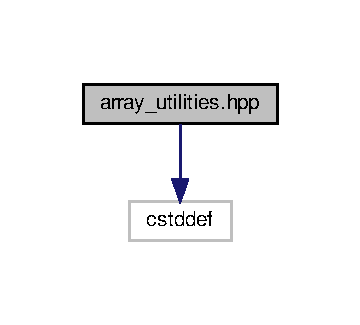
\includegraphics[width=173pt]{array__utilities_8hpp__incl}
\end{center}
\end{figure}
This graph shows which files directly or indirectly include this file\+:\nopagebreak
\begin{figure}[H]
\begin{center}
\leavevmode
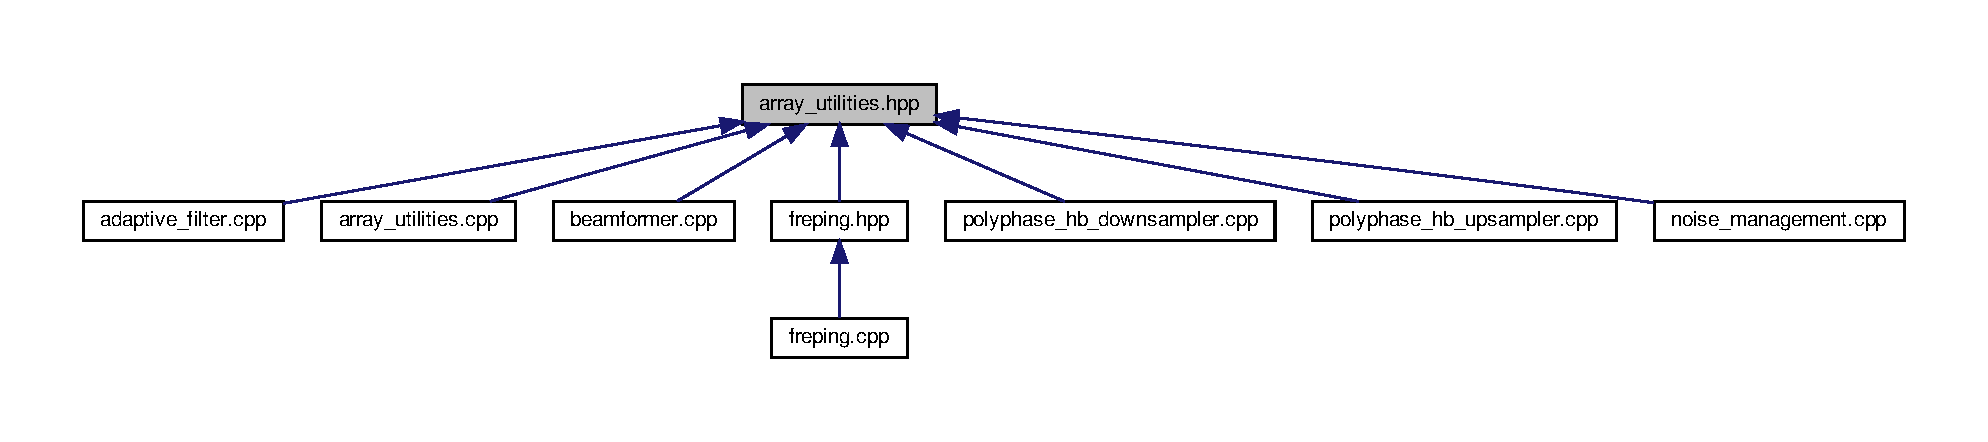
\includegraphics[width=350pt]{array__utilities_8hpp__dep__incl}
\end{center}
\end{figure}
\subsection*{Functions}
\begin{DoxyCompactItemize}
\item 
void \hyperlink{array__utilities_8hpp_a671b885d4bc80890d5db79251c179cc6}{array\+\_\+flip} (float $\ast$arr, size\+\_\+t len)
\begin{DoxyCompactList}\small\item\em Function to reverse an array. \end{DoxyCompactList}\item 
float \hyperlink{array__utilities_8hpp_a951da7a6e40691865c6b669e65235848}{array\+\_\+sum} (const float $\ast$arr, size\+\_\+t len)
\begin{DoxyCompactList}\small\item\em Function to calculate the sum of an array. \end{DoxyCompactList}\item 
float \hyperlink{array__utilities_8hpp_a553c08dad0548039a851968d25767881}{array\+\_\+dot\+\_\+product} (const float $\ast$in1, const float $\ast$in2, size\+\_\+t len)
\begin{DoxyCompactList}\small\item\em Function to calculate the dot-\/product of two 1-\/D vectors/arrays. \end{DoxyCompactList}\item 
void \hyperlink{array__utilities_8hpp_ac5e150940a31a2aace5bc977dfed62e7}{array\+\_\+right\+\_\+shift} (float $\ast$arr, size\+\_\+t len)
\begin{DoxyCompactList}\small\item\em Function to right shift an array by one place. Left most value will be replaced by zero. \end{DoxyCompactList}\item 
void \hyperlink{array__utilities_8hpp_ae9c0f53e57eba1f9b68b3b98035c7104}{array\+\_\+multiply\+\_\+const} (float $\ast$arr, float constant, size\+\_\+t len)
\begin{DoxyCompactList}\small\item\em Function to multiply each element of an array by a scalar constant. \end{DoxyCompactList}\item 
void \hyperlink{array__utilities_8hpp_ac5021e5ce6e8fbcdefd4ec345304363e}{array\+\_\+add\+\_\+const} (float $\ast$arr, float constant, size\+\_\+t len)
\begin{DoxyCompactList}\small\item\em Function to add a scalar constant to each element of an array. \end{DoxyCompactList}\item 
void \hyperlink{array__utilities_8hpp_aeb83126cafbf7b72e9c4229b630f93f7}{array\+\_\+add\+\_\+array} (float $\ast$in1, const float $\ast$in2, size\+\_\+t len)
\begin{DoxyCompactList}\small\item\em Function to do element wise addition of two arrays. \end{DoxyCompactList}\item 
void \hyperlink{array__utilities_8hpp_a16c4485ad0fc4addbd8e4966b6c2dd34}{array\+\_\+subtract\+\_\+array} (float $\ast$in1, const float $\ast$in2, size\+\_\+t len)
\begin{DoxyCompactList}\small\item\em Function to do element wise subtraction of two arrays. \end{DoxyCompactList}\item 
void \hyperlink{array__utilities_8hpp_a5d18621319de15256d97586e9be833b5}{array\+\_\+element\+\_\+multiply\+\_\+array} (float $\ast$in1, const float $\ast$in2, size\+\_\+t len)
\begin{DoxyCompactList}\small\item\em Function to do element wise multiplication of two arrays. \end{DoxyCompactList}\item 
void \hyperlink{array__utilities_8hpp_ace8a12bb47149c5215616caf9dd5d594}{array\+\_\+element\+\_\+divide\+\_\+array} (float $\ast$in1, const float $\ast$in2, size\+\_\+t len)
\begin{DoxyCompactList}\small\item\em Function to do element wise division of two arrays. \end{DoxyCompactList}\item 
float \hyperlink{array__utilities_8hpp_a9a766be2ca62f99e043583cd6ae183fc}{array\+\_\+min} (const float $\ast$arr, size\+\_\+t len)
\begin{DoxyCompactList}\small\item\em Function to return the minimum of the elements of an array. \end{DoxyCompactList}\item 
float \hyperlink{array__utilities_8hpp_abd95915e71cdf97c66dd2092aed740df}{array\+\_\+mean} (float $\ast$arr, size\+\_\+t len)
\begin{DoxyCompactList}\small\item\em Function to calculate the mean of the elements of an array. \end{DoxyCompactList}\item 
void \hyperlink{array__utilities_8hpp_a41f17b8ac6c9f77c6bc16231a35b0304}{array\+\_\+square} (const float $\ast$in, float $\ast$out, size\+\_\+t len)
\begin{DoxyCompactList}\small\item\em Function to populate the output array with square of the elements of an input array. \end{DoxyCompactList}\item 
float \hyperlink{array__utilities_8hpp_a7adedf9123b714557d3d35ed500d82b9}{array\+\_\+mean\+\_\+square} (const float $\ast$arr, size\+\_\+t len)
\begin{DoxyCompactList}\small\item\em Function to calculate the mean square of the elements of an array. \end{DoxyCompactList}\item 
void \hyperlink{array__utilities_8hpp_ad1f8261eef0b72711c198bdc73fb934d}{array\+\_\+print} (const char $\ast$str, float $\ast$arr, size\+\_\+t len)
\begin{DoxyCompactList}\small\item\em Function to print an array for debugging. \end{DoxyCompactList}\end{DoxyCompactItemize}


\subsection{Detailed Description}
\begin{DoxyAuthor}{Author}
Open Speech Platform (O\+SP) Team, U\+C\+SD 
\end{DoxyAuthor}
\begin{DoxyCopyright}{Copyright}
Copyright (C) 2020 Regents of the University of California Redistribution and use in source and binary forms, with or without modification, are permitted provided that the following conditions are met\+: \begin{DoxyVerb}1. Redistributions of source code must retain the above copyright notice, this list of conditions and the
following disclaimer.

2. Redistributions in binary form must reproduce the above copyright notice, this list of conditions and the
following disclaimer in the documentation and/or other materials provided with the distribution.
\end{DoxyVerb}

\end{DoxyCopyright}
T\+H\+IS S\+O\+F\+T\+W\+A\+RE IS P\+R\+O\+V\+I\+D\+ED BY T\+HE C\+O\+P\+Y\+R\+I\+G\+HT H\+O\+L\+D\+E\+RS A\+ND C\+O\+N\+T\+R\+I\+B\+U\+T\+O\+RS \char`\"{}\+A\+S I\+S\char`\"{} A\+ND A\+NY E\+X\+P\+R\+E\+SS OR I\+M\+P\+L\+I\+ED W\+A\+R\+R\+A\+N\+T\+I\+ES, I\+N\+C\+L\+U\+D\+I\+NG, B\+UT N\+OT L\+I\+M\+I\+T\+ED TO, T\+HE I\+M\+P\+L\+I\+ED W\+A\+R\+R\+A\+N\+T\+I\+ES OF M\+E\+R\+C\+H\+A\+N\+T\+A\+B\+I\+L\+I\+TY A\+ND F\+I\+T\+N\+E\+SS F\+OR A P\+A\+R\+T\+I\+C\+U\+L\+AR P\+U\+R\+P\+O\+SE A\+RE D\+I\+S\+C\+L\+A\+I\+M\+ED. IN NO E\+V\+E\+NT S\+H\+A\+LL T\+HE C\+O\+P\+Y\+R\+I\+G\+HT H\+O\+L\+D\+ER OR C\+O\+N\+T\+R\+I\+B\+U\+T\+O\+RS BE L\+I\+A\+B\+LE F\+OR A\+NY D\+I\+R\+E\+CT, I\+N\+D\+I\+R\+E\+CT, I\+N\+C\+I\+D\+E\+N\+T\+AL, S\+P\+E\+C\+I\+AL, E\+X\+E\+M\+P\+L\+A\+RY, OR C\+O\+N\+S\+E\+Q\+U\+E\+N\+T\+I\+AL D\+A\+M\+A\+G\+ES (I\+N\+C\+L\+U\+D\+I\+NG, B\+UT N\+OT L\+I\+M\+I\+T\+ED TO, P\+R\+O\+C\+U\+R\+E\+M\+E\+NT OF S\+U\+B\+S\+T\+I\+T\+U\+TE G\+O\+O\+DS OR S\+E\+R\+V\+I\+C\+ES; L\+O\+SS OF U\+SE, D\+A\+TA, OR P\+R\+O\+F\+I\+TS; OR B\+U\+S\+I\+N\+E\+SS I\+N\+T\+E\+R\+R\+U\+P\+T\+I\+ON) H\+O\+W\+E\+V\+ER C\+A\+U\+S\+ED A\+ND ON A\+NY T\+H\+E\+O\+RY OF L\+I\+A\+B\+I\+L\+I\+TY, W\+H\+E\+T\+H\+ER IN C\+O\+N\+T\+R\+A\+CT, S\+T\+R\+I\+CT L\+I\+A\+B\+I\+L\+I\+TY, OR T\+O\+RT (I\+N\+C\+L\+U\+D\+I\+NG N\+E\+G\+L\+I\+G\+E\+N\+CE OR O\+T\+H\+E\+R\+W\+I\+SE) A\+R\+I\+S\+I\+NG IN A\+NY W\+AY O\+UT OF T\+HE U\+SE OF T\+H\+IS S\+O\+F\+T\+W\+A\+RE, E\+V\+EN IF A\+D\+V\+I\+S\+ED OF T\+HE P\+O\+S\+S\+I\+B\+I\+L\+I\+TY OF S\+U\+CH D\+A\+M\+A\+GE.

\subsection{Function Documentation}
\mbox{\Hypertarget{array__utilities_8hpp_aeb83126cafbf7b72e9c4229b630f93f7}\label{array__utilities_8hpp_aeb83126cafbf7b72e9c4229b630f93f7}} 
\index{array\+\_\+utilities.\+hpp@{array\+\_\+utilities.\+hpp}!array\+\_\+add\+\_\+array@{array\+\_\+add\+\_\+array}}
\index{array\+\_\+add\+\_\+array@{array\+\_\+add\+\_\+array}!array\+\_\+utilities.\+hpp@{array\+\_\+utilities.\+hpp}}
\subsubsection{\texorpdfstring{array\+\_\+add\+\_\+array()}{array\_add\_array()}}
{\footnotesize\ttfamily void array\+\_\+add\+\_\+array (\begin{DoxyParamCaption}\item[{float $\ast$}]{in1,  }\item[{const float $\ast$}]{in2,  }\item[{size\+\_\+t}]{len }\end{DoxyParamCaption})}



Function to do element wise addition of two arrays. 


\begin{DoxyParams}{Parameters}
{\em in1} & Pointer to the first array \\
\hline
{\em in2} & Pointer to the second array \\
\hline
{\em len} & Length of the arrays \\
\hline
\end{DoxyParams}
\begin{DoxyWarning}{Warning}
Assumes both the arrays are of same length and takes only one length parameter 
\end{DoxyWarning}


Definition at line 105 of file array\+\_\+utilities.\+cpp.

\mbox{\Hypertarget{array__utilities_8hpp_ac5021e5ce6e8fbcdefd4ec345304363e}\label{array__utilities_8hpp_ac5021e5ce6e8fbcdefd4ec345304363e}} 
\index{array\+\_\+utilities.\+hpp@{array\+\_\+utilities.\+hpp}!array\+\_\+add\+\_\+const@{array\+\_\+add\+\_\+const}}
\index{array\+\_\+add\+\_\+const@{array\+\_\+add\+\_\+const}!array\+\_\+utilities.\+hpp@{array\+\_\+utilities.\+hpp}}
\subsubsection{\texorpdfstring{array\+\_\+add\+\_\+const()}{array\_add\_const()}}
{\footnotesize\ttfamily void array\+\_\+add\+\_\+const (\begin{DoxyParamCaption}\item[{float $\ast$}]{arr,  }\item[{float}]{constant,  }\item[{size\+\_\+t}]{len }\end{DoxyParamCaption})}



Function to add a scalar constant to each element of an array. 


\begin{DoxyParams}{Parameters}
{\em arr} & Pointer to the array \\
\hline
{\em constant} & The constant scalar adder \\
\hline
{\em len} & Length of the array \\
\hline
\end{DoxyParams}


Definition at line 96 of file array\+\_\+utilities.\+cpp.

\mbox{\Hypertarget{array__utilities_8hpp_a553c08dad0548039a851968d25767881}\label{array__utilities_8hpp_a553c08dad0548039a851968d25767881}} 
\index{array\+\_\+utilities.\+hpp@{array\+\_\+utilities.\+hpp}!array\+\_\+dot\+\_\+product@{array\+\_\+dot\+\_\+product}}
\index{array\+\_\+dot\+\_\+product@{array\+\_\+dot\+\_\+product}!array\+\_\+utilities.\+hpp@{array\+\_\+utilities.\+hpp}}
\subsubsection{\texorpdfstring{array\+\_\+dot\+\_\+product()}{array\_dot\_product()}}
{\footnotesize\ttfamily float array\+\_\+dot\+\_\+product (\begin{DoxyParamCaption}\item[{const float $\ast$}]{in1,  }\item[{const float $\ast$}]{in2,  }\item[{size\+\_\+t}]{len }\end{DoxyParamCaption})}



Function to calculate the dot-\/product of two 1-\/D vectors/arrays. 


\begin{DoxyParams}{Parameters}
{\em in1} & Pointer to the first vector \\
\hline
{\em in2} & Pointer to the second vector \\
\hline
{\em len} & Length of the vectors \\
\hline
\end{DoxyParams}
\begin{DoxyReturn}{Returns}
Dot product (inner product) of the two vectors 
\end{DoxyReturn}
\begin{DoxyWarning}{Warning}
Assumes both the vectors are of same length and takes only one length parameter 
\end{DoxyWarning}


Definition at line 67 of file array\+\_\+utilities.\+cpp.

\mbox{\Hypertarget{array__utilities_8hpp_ace8a12bb47149c5215616caf9dd5d594}\label{array__utilities_8hpp_ace8a12bb47149c5215616caf9dd5d594}} 
\index{array\+\_\+utilities.\+hpp@{array\+\_\+utilities.\+hpp}!array\+\_\+element\+\_\+divide\+\_\+array@{array\+\_\+element\+\_\+divide\+\_\+array}}
\index{array\+\_\+element\+\_\+divide\+\_\+array@{array\+\_\+element\+\_\+divide\+\_\+array}!array\+\_\+utilities.\+hpp@{array\+\_\+utilities.\+hpp}}
\subsubsection{\texorpdfstring{array\+\_\+element\+\_\+divide\+\_\+array()}{array\_element\_divide\_array()}}
{\footnotesize\ttfamily void array\+\_\+element\+\_\+divide\+\_\+array (\begin{DoxyParamCaption}\item[{float $\ast$}]{in1,  }\item[{const float $\ast$}]{in2,  }\item[{size\+\_\+t}]{len }\end{DoxyParamCaption})}



Function to do element wise division of two arrays. 


\begin{DoxyParams}{Parameters}
{\em in1} & Pointer to the first array \\
\hline
{\em in2} & Pointer to the second array \\
\hline
{\em len} & Length of the arrays \\
\hline
\end{DoxyParams}
\begin{DoxyWarning}{Warning}
Assumes both the arrays are of same length and takes only one length parameter 
\end{DoxyWarning}


Definition at line 132 of file array\+\_\+utilities.\+cpp.

\mbox{\Hypertarget{array__utilities_8hpp_a5d18621319de15256d97586e9be833b5}\label{array__utilities_8hpp_a5d18621319de15256d97586e9be833b5}} 
\index{array\+\_\+utilities.\+hpp@{array\+\_\+utilities.\+hpp}!array\+\_\+element\+\_\+multiply\+\_\+array@{array\+\_\+element\+\_\+multiply\+\_\+array}}
\index{array\+\_\+element\+\_\+multiply\+\_\+array@{array\+\_\+element\+\_\+multiply\+\_\+array}!array\+\_\+utilities.\+hpp@{array\+\_\+utilities.\+hpp}}
\subsubsection{\texorpdfstring{array\+\_\+element\+\_\+multiply\+\_\+array()}{array\_element\_multiply\_array()}}
{\footnotesize\ttfamily void array\+\_\+element\+\_\+multiply\+\_\+array (\begin{DoxyParamCaption}\item[{float $\ast$}]{in1,  }\item[{const float $\ast$}]{in2,  }\item[{size\+\_\+t}]{len }\end{DoxyParamCaption})}



Function to do element wise multiplication of two arrays. 


\begin{DoxyParams}{Parameters}
{\em in1} & Pointer to the first array \\
\hline
{\em in2} & Pointer to the second array \\
\hline
{\em len} & Length of the arrays \\
\hline
\end{DoxyParams}
\begin{DoxyWarning}{Warning}
Assumes both the arrays are of same length and takes only one length parameter 
\end{DoxyWarning}


Definition at line 123 of file array\+\_\+utilities.\+cpp.

\mbox{\Hypertarget{array__utilities_8hpp_a671b885d4bc80890d5db79251c179cc6}\label{array__utilities_8hpp_a671b885d4bc80890d5db79251c179cc6}} 
\index{array\+\_\+utilities.\+hpp@{array\+\_\+utilities.\+hpp}!array\+\_\+flip@{array\+\_\+flip}}
\index{array\+\_\+flip@{array\+\_\+flip}!array\+\_\+utilities.\+hpp@{array\+\_\+utilities.\+hpp}}
\subsubsection{\texorpdfstring{array\+\_\+flip()}{array\_flip()}}
{\footnotesize\ttfamily void array\+\_\+flip (\begin{DoxyParamCaption}\item[{float $\ast$}]{arr,  }\item[{size\+\_\+t}]{len }\end{DoxyParamCaption})}



Function to reverse an array. 


\begin{DoxyParams}{Parameters}
{\em arr} & Pointer to the array \\
\hline
{\em len} & Length of the array \\
\hline
\end{DoxyParams}


Definition at line 31 of file array\+\_\+utilities.\+cpp.

\mbox{\Hypertarget{array__utilities_8hpp_abd95915e71cdf97c66dd2092aed740df}\label{array__utilities_8hpp_abd95915e71cdf97c66dd2092aed740df}} 
\index{array\+\_\+utilities.\+hpp@{array\+\_\+utilities.\+hpp}!array\+\_\+mean@{array\+\_\+mean}}
\index{array\+\_\+mean@{array\+\_\+mean}!array\+\_\+utilities.\+hpp@{array\+\_\+utilities.\+hpp}}
\subsubsection{\texorpdfstring{array\+\_\+mean()}{array\_mean()}}
{\footnotesize\ttfamily float array\+\_\+mean (\begin{DoxyParamCaption}\item[{float $\ast$}]{arr,  }\item[{size\+\_\+t}]{len }\end{DoxyParamCaption})}



Function to calculate the mean of the elements of an array. 


\begin{DoxyParams}{Parameters}
{\em arr} & Pointer to the array \\
\hline
{\em len} & Length of the array \\
\hline
\end{DoxyParams}
\begin{DoxyReturn}{Returns}
Mean of the array elements 
\end{DoxyReturn}


Definition at line 156 of file array\+\_\+utilities.\+cpp.

\mbox{\Hypertarget{array__utilities_8hpp_a7adedf9123b714557d3d35ed500d82b9}\label{array__utilities_8hpp_a7adedf9123b714557d3d35ed500d82b9}} 
\index{array\+\_\+utilities.\+hpp@{array\+\_\+utilities.\+hpp}!array\+\_\+mean\+\_\+square@{array\+\_\+mean\+\_\+square}}
\index{array\+\_\+mean\+\_\+square@{array\+\_\+mean\+\_\+square}!array\+\_\+utilities.\+hpp@{array\+\_\+utilities.\+hpp}}
\subsubsection{\texorpdfstring{array\+\_\+mean\+\_\+square()}{array\_mean\_square()}}
{\footnotesize\ttfamily float array\+\_\+mean\+\_\+square (\begin{DoxyParamCaption}\item[{const float $\ast$}]{arr,  }\item[{size\+\_\+t}]{len }\end{DoxyParamCaption})}



Function to calculate the mean square of the elements of an array. 


\begin{DoxyParams}{Parameters}
{\em arr} & Pointer to the array \\
\hline
{\em len} & Length of the array \\
\hline
\end{DoxyParams}
\begin{DoxyReturn}{Returns}
Mean square of the array elements 
\end{DoxyReturn}


Definition at line 172 of file array\+\_\+utilities.\+cpp.

\mbox{\Hypertarget{array__utilities_8hpp_a9a766be2ca62f99e043583cd6ae183fc}\label{array__utilities_8hpp_a9a766be2ca62f99e043583cd6ae183fc}} 
\index{array\+\_\+utilities.\+hpp@{array\+\_\+utilities.\+hpp}!array\+\_\+min@{array\+\_\+min}}
\index{array\+\_\+min@{array\+\_\+min}!array\+\_\+utilities.\+hpp@{array\+\_\+utilities.\+hpp}}
\subsubsection{\texorpdfstring{array\+\_\+min()}{array\_min()}}
{\footnotesize\ttfamily float array\+\_\+min (\begin{DoxyParamCaption}\item[{const float $\ast$}]{arr,  }\item[{size\+\_\+t}]{len }\end{DoxyParamCaption})}



Function to return the minimum of the elements of an array. 


\begin{DoxyParams}{Parameters}
{\em arr} & Pointer to the array \\
\hline
{\em len} & Length of the array \\
\hline
\end{DoxyParams}
\begin{DoxyReturn}{Returns}
Minimum of the array elements 
\end{DoxyReturn}


Definition at line 141 of file array\+\_\+utilities.\+cpp.

\mbox{\Hypertarget{array__utilities_8hpp_ae9c0f53e57eba1f9b68b3b98035c7104}\label{array__utilities_8hpp_ae9c0f53e57eba1f9b68b3b98035c7104}} 
\index{array\+\_\+utilities.\+hpp@{array\+\_\+utilities.\+hpp}!array\+\_\+multiply\+\_\+const@{array\+\_\+multiply\+\_\+const}}
\index{array\+\_\+multiply\+\_\+const@{array\+\_\+multiply\+\_\+const}!array\+\_\+utilities.\+hpp@{array\+\_\+utilities.\+hpp}}
\subsubsection{\texorpdfstring{array\+\_\+multiply\+\_\+const()}{array\_multiply\_const()}}
{\footnotesize\ttfamily void array\+\_\+multiply\+\_\+const (\begin{DoxyParamCaption}\item[{float $\ast$}]{arr,  }\item[{float}]{constant,  }\item[{size\+\_\+t}]{len }\end{DoxyParamCaption})}



Function to multiply each element of an array by a scalar constant. 


\begin{DoxyParams}{Parameters}
{\em arr} & Pointer to the array \\
\hline
{\em constant} & The constant scalar multiplier \\
\hline
{\em len} & Length of the array \\
\hline
\end{DoxyParams}


Definition at line 87 of file array\+\_\+utilities.\+cpp.

\mbox{\Hypertarget{array__utilities_8hpp_ad1f8261eef0b72711c198bdc73fb934d}\label{array__utilities_8hpp_ad1f8261eef0b72711c198bdc73fb934d}} 
\index{array\+\_\+utilities.\+hpp@{array\+\_\+utilities.\+hpp}!array\+\_\+print@{array\+\_\+print}}
\index{array\+\_\+print@{array\+\_\+print}!array\+\_\+utilities.\+hpp@{array\+\_\+utilities.\+hpp}}
\subsubsection{\texorpdfstring{array\+\_\+print()}{array\_print()}}
{\footnotesize\ttfamily void array\+\_\+print (\begin{DoxyParamCaption}\item[{const char $\ast$}]{str,  }\item[{float $\ast$}]{arr,  }\item[{size\+\_\+t}]{len }\end{DoxyParamCaption})}



Function to print an array for debugging. 


\begin{DoxyParams}{Parameters}
{\em str} & String to use for debugging \\
\hline
{\em arr} & Pointer to the array \\
\hline
{\em len} & Length of the array \\
\hline
\end{DoxyParams}


Definition at line 177 of file array\+\_\+utilities.\+cpp.

\mbox{\Hypertarget{array__utilities_8hpp_ac5e150940a31a2aace5bc977dfed62e7}\label{array__utilities_8hpp_ac5e150940a31a2aace5bc977dfed62e7}} 
\index{array\+\_\+utilities.\+hpp@{array\+\_\+utilities.\+hpp}!array\+\_\+right\+\_\+shift@{array\+\_\+right\+\_\+shift}}
\index{array\+\_\+right\+\_\+shift@{array\+\_\+right\+\_\+shift}!array\+\_\+utilities.\+hpp@{array\+\_\+utilities.\+hpp}}
\subsubsection{\texorpdfstring{array\+\_\+right\+\_\+shift()}{array\_right\_shift()}}
{\footnotesize\ttfamily void array\+\_\+right\+\_\+shift (\begin{DoxyParamCaption}\item[{float $\ast$}]{arr,  }\item[{size\+\_\+t}]{len }\end{DoxyParamCaption})}



Function to right shift an array by one place. Left most value will be replaced by zero. 


\begin{DoxyParams}{Parameters}
{\em arr} & Pointer to the array \\
\hline
{\em len} & Length of the array \\
\hline
\end{DoxyParams}


Definition at line 78 of file array\+\_\+utilities.\+cpp.

\mbox{\Hypertarget{array__utilities_8hpp_a41f17b8ac6c9f77c6bc16231a35b0304}\label{array__utilities_8hpp_a41f17b8ac6c9f77c6bc16231a35b0304}} 
\index{array\+\_\+utilities.\+hpp@{array\+\_\+utilities.\+hpp}!array\+\_\+square@{array\+\_\+square}}
\index{array\+\_\+square@{array\+\_\+square}!array\+\_\+utilities.\+hpp@{array\+\_\+utilities.\+hpp}}
\subsubsection{\texorpdfstring{array\+\_\+square()}{array\_square()}}
{\footnotesize\ttfamily void array\+\_\+square (\begin{DoxyParamCaption}\item[{const float $\ast$}]{in,  }\item[{float $\ast$}]{out,  }\item[{size\+\_\+t}]{len }\end{DoxyParamCaption})}



Function to populate the output array with square of the elements of an input array. 


\begin{DoxyParams}{Parameters}
{\em in} & Pointer to the input array \\
\hline
{\em out} & Pointer to the output array \\
\hline
{\em len} & Length of the arrays \\
\hline
\end{DoxyParams}
\begin{DoxyWarning}{Warning}
Assumes that output array already has memory allocated to it 
\end{DoxyWarning}


Definition at line 163 of file array\+\_\+utilities.\+cpp.

\mbox{\Hypertarget{array__utilities_8hpp_a16c4485ad0fc4addbd8e4966b6c2dd34}\label{array__utilities_8hpp_a16c4485ad0fc4addbd8e4966b6c2dd34}} 
\index{array\+\_\+utilities.\+hpp@{array\+\_\+utilities.\+hpp}!array\+\_\+subtract\+\_\+array@{array\+\_\+subtract\+\_\+array}}
\index{array\+\_\+subtract\+\_\+array@{array\+\_\+subtract\+\_\+array}!array\+\_\+utilities.\+hpp@{array\+\_\+utilities.\+hpp}}
\subsubsection{\texorpdfstring{array\+\_\+subtract\+\_\+array()}{array\_subtract\_array()}}
{\footnotesize\ttfamily void array\+\_\+subtract\+\_\+array (\begin{DoxyParamCaption}\item[{float $\ast$}]{in1,  }\item[{const float $\ast$}]{in2,  }\item[{size\+\_\+t}]{len }\end{DoxyParamCaption})}



Function to do element wise subtraction of two arrays. 


\begin{DoxyParams}{Parameters}
{\em in1} & Pointer to the first array \\
\hline
{\em in2} & Pointer to the second array \\
\hline
{\em len} & Length of the arrays \\
\hline
\end{DoxyParams}
\begin{DoxyWarning}{Warning}
Assumes both the arrays are of same length and takes only one length parameter 
\end{DoxyWarning}


Definition at line 114 of file array\+\_\+utilities.\+cpp.

\mbox{\Hypertarget{array__utilities_8hpp_a951da7a6e40691865c6b669e65235848}\label{array__utilities_8hpp_a951da7a6e40691865c6b669e65235848}} 
\index{array\+\_\+utilities.\+hpp@{array\+\_\+utilities.\+hpp}!array\+\_\+sum@{array\+\_\+sum}}
\index{array\+\_\+sum@{array\+\_\+sum}!array\+\_\+utilities.\+hpp@{array\+\_\+utilities.\+hpp}}
\subsubsection{\texorpdfstring{array\+\_\+sum()}{array\_sum()}}
{\footnotesize\ttfamily float array\+\_\+sum (\begin{DoxyParamCaption}\item[{const float $\ast$}]{arr,  }\item[{size\+\_\+t}]{len }\end{DoxyParamCaption})}



Function to calculate the sum of an array. 


\begin{DoxyParams}{Parameters}
{\em arr} & Pointer to the array \\
\hline
{\em len} & Length of the array \\
\hline
\end{DoxyParams}
\begin{DoxyReturn}{Returns}
Sum of the array 
\end{DoxyReturn}


Definition at line 47 of file array\+\_\+utilities.\+cpp.


\hypertarget{AudioFile_8cpp}{}\section{Audio\+File.\+cpp File Reference}
\label{AudioFile_8cpp}\index{Audio\+File.\+cpp@{Audio\+File.\+cpp}}
{\ttfamily \#include \char`\"{}Audio\+File.\+h\char`\"{}}\newline
{\ttfamily \#include $<$fstream$>$}\newline
{\ttfamily \#include $<$unordered\+\_\+map$>$}\newline
{\ttfamily \#include $<$iterator$>$}\newline
Include dependency graph for Audio\+File.\+cpp\+:\nopagebreak
\begin{figure}[H]
\begin{center}
\leavevmode
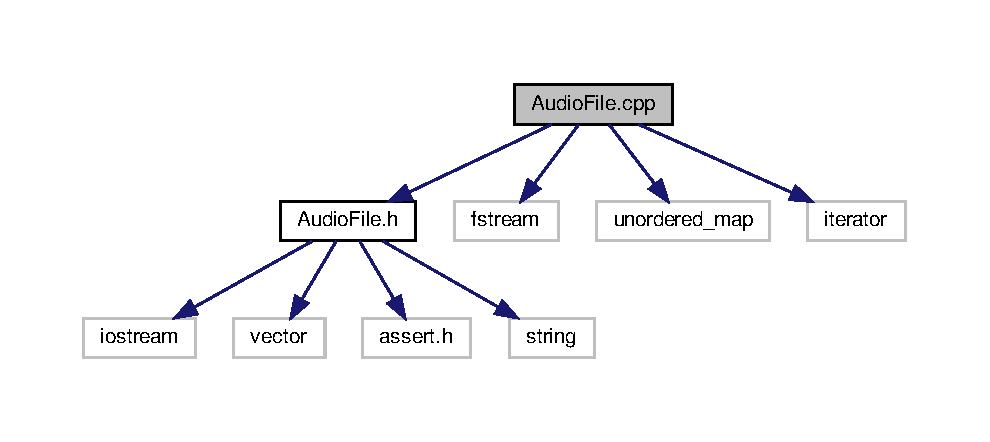
\includegraphics[width=350pt]{AudioFile_8cpp__incl}
\end{center}
\end{figure}
\subsection*{Variables}
\begin{DoxyCompactItemize}
\item 
std\+::unordered\+\_\+map$<$ uint32\+\_\+t, std\+::vector$<$ uint8\+\_\+t $>$ $>$ {\bfseries aiff\+Sample\+Rate\+Table}
\end{DoxyCompactItemize}


\subsection{Detailed Description}
\begin{DoxyAuthor}{Author}
Adam Stark 
\end{DoxyAuthor}
\begin{DoxyCopyright}{Copyright}
Copyright (C) 2017 Adam Stark
\end{DoxyCopyright}
This file is part of the \textquotesingle{}\hyperlink{classAudioFile}{Audio\+File}\textquotesingle{} library

This program is free software\+: you can redistribute it and/or modify it under the terms of the G\+NU General Public License as published by the Free Software Foundation, either version 3 of the License, or (at your option) any later version.

This program is distributed in the hope that it will be useful, but W\+I\+T\+H\+O\+UT A\+NY W\+A\+R\+R\+A\+N\+TY; without even the implied warranty of M\+E\+R\+C\+H\+A\+N\+T\+A\+B\+I\+L\+I\+TY or F\+I\+T\+N\+E\+SS F\+OR A P\+A\+R\+T\+I\+C\+U\+L\+AR P\+U\+R\+P\+O\+SE. See the G\+NU General Public License for more details.

You should have received a copy of the G\+NU General Public License along with this program. If not, see \href{http://www.gnu.org/licenses/}{\tt http\+://www.\+gnu.\+org/licenses/}. 

\subsection{Variable Documentation}
\mbox{\Hypertarget{AudioFile_8cpp_abf9b30998d0448afa3d74af3ac87eb67}\label{AudioFile_8cpp_abf9b30998d0448afa3d74af3ac87eb67}} 
\index{Audio\+File.\+cpp@{Audio\+File.\+cpp}!aiff\+Sample\+Rate\+Table@{aiff\+Sample\+Rate\+Table}}
\index{aiff\+Sample\+Rate\+Table@{aiff\+Sample\+Rate\+Table}!Audio\+File.\+cpp@{Audio\+File.\+cpp}}
\subsubsection{\texorpdfstring{aiff\+Sample\+Rate\+Table}{aiffSampleRateTable}}
{\footnotesize\ttfamily std\+::unordered\+\_\+map$<$uint32\+\_\+t, std\+::vector$<$uint8\+\_\+t$>$ $>$ aiff\+Sample\+Rate\+Table}

{\bfseries Initial value\+:}
\begin{DoxyCode}
= \{
    \{8000, \{64, 11, 250, 0, 0, 0, 0, 0, 0, 0\}\},
    \{11025, \{64, 12, 172, 68, 0, 0, 0, 0, 0, 0\}\},
    \{16000, \{64, 12, 250, 0, 0, 0, 0, 0, 0, 0\}\},
    \{22050, \{64, 13, 172, 68, 0, 0, 0, 0, 0, 0\}\},
    \{32000, \{64, 13, 250, 0, 0, 0, 0, 0, 0, 0\}\},
    \{37800, \{64, 14, 147, 168, 0, 0, 0, 0, 0, 0\}\},
    \{44056, \{64, 14, 172, 24, 0, 0, 0, 0, 0, 0\}\},
    \{44100, \{64, 14, 172, 68, 0, 0, 0, 0, 0, 0\}\},
    \{47250, \{64, 14, 184, 146, 0, 0, 0, 0, 0, 0\}\},
    \{48000, \{64, 14, 187, 128, 0, 0, 0, 0, 0, 0\}\},
    \{50000, \{64, 14, 195, 80, 0, 0, 0, 0, 0, 0\}\},
    \{50400, \{64, 14, 196, 224, 0, 0, 0, 0, 0, 0\}\},
    \{88200, \{64, 15, 172, 68, 0, 0, 0, 0, 0, 0\}\},
    \{96000, \{64, 15, 187, 128, 0, 0, 0, 0, 0, 0\}\},
    \{176400, \{64, 16, 172, 68, 0, 0, 0, 0, 0, 0\}\},
    \{192000, \{64, 16, 187, 128, 0, 0, 0, 0, 0, 0\}\},
    \{352800, \{64, 17, 172, 68, 0, 0, 0, 0, 0, 0\}\},
    \{2822400, \{64, 20, 172, 68, 0, 0, 0, 0, 0, 0\}\},
    \{5644800, \{64, 21, 172, 68, 0, 0, 0, 0, 0, 0\}\}
\}
\end{DoxyCode}


Definition at line 30 of file Audio\+File.\+cpp.


\hypertarget{AudioFile_8h}{}\section{Audio\+File.\+h File Reference}
\label{AudioFile_8h}\index{Audio\+File.\+h@{Audio\+File.\+h}}
{\ttfamily \#include $<$iostream$>$}\newline
{\ttfamily \#include $<$vector$>$}\newline
{\ttfamily \#include $<$assert.\+h$>$}\newline
{\ttfamily \#include $<$string$>$}\newline
Include dependency graph for Audio\+File.\+h\+:\nopagebreak
\begin{figure}[H]
\begin{center}
\leavevmode
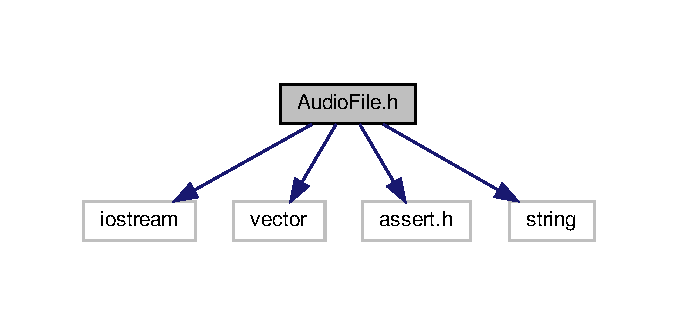
\includegraphics[width=326pt]{AudioFile_8h__incl}
\end{center}
\end{figure}
This graph shows which files directly or indirectly include this file\+:\nopagebreak
\begin{figure}[H]
\begin{center}
\leavevmode
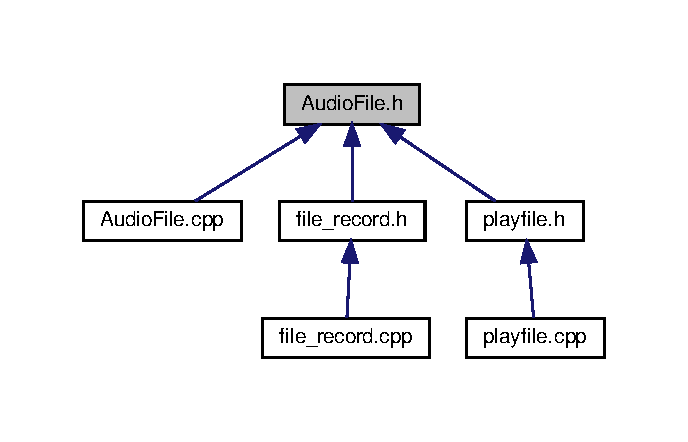
\includegraphics[width=330pt]{AudioFile_8h__dep__incl}
\end{center}
\end{figure}
\subsection*{Classes}
\begin{DoxyCompactItemize}
\item 
class \hyperlink{classAudioFile}{Audio\+File$<$ T $>$}
\end{DoxyCompactItemize}
\subsection*{Enumerations}
\begin{DoxyCompactItemize}
\item 
enum \hyperlink{AudioFile_8h_ad18559d169602e85d0ad68da6ef8593f}{Audio\+File\+Format} \{ {\bfseries Error}, 
{\bfseries Not\+Loaded}, 
{\bfseries Wave}, 
{\bfseries Aiff}
 \}
\end{DoxyCompactItemize}


\subsection{Detailed Description}
\begin{DoxyAuthor}{Author}
Adam Stark 
\end{DoxyAuthor}
\begin{DoxyCopyright}{Copyright}
Copyright (C) 2017 Adam Stark
\end{DoxyCopyright}
This file is part of the \textquotesingle{}\hyperlink{classAudioFile}{Audio\+File}\textquotesingle{} library

This program is free software\+: you can redistribute it and/or modify it under the terms of the G\+NU General Public License as published by the Free Software Foundation, either version 3 of the License, or (at your option) any later version.

This program is distributed in the hope that it will be useful, but W\+I\+T\+H\+O\+UT A\+NY W\+A\+R\+R\+A\+N\+TY; without even the implied warranty of M\+E\+R\+C\+H\+A\+N\+T\+A\+B\+I\+L\+I\+TY or F\+I\+T\+N\+E\+SS F\+OR A P\+A\+R\+T\+I\+C\+U\+L\+AR P\+U\+R\+P\+O\+SE. See the G\+NU General Public License for more details.

You should have received a copy of the G\+NU General Public License along with this program. If not, see \href{http://www.gnu.org/licenses/}{\tt http\+://www.\+gnu.\+org/licenses/}. 

\subsection{Enumeration Type Documentation}
\mbox{\Hypertarget{AudioFile_8h_ad18559d169602e85d0ad68da6ef8593f}\label{AudioFile_8h_ad18559d169602e85d0ad68da6ef8593f}} 
\index{Audio\+File.\+h@{Audio\+File.\+h}!Audio\+File\+Format@{Audio\+File\+Format}}
\index{Audio\+File\+Format@{Audio\+File\+Format}!Audio\+File.\+h@{Audio\+File.\+h}}
\subsubsection{\texorpdfstring{Audio\+File\+Format}{AudioFileFormat}}
{\footnotesize\ttfamily enum \hyperlink{AudioFile_8h_ad18559d169602e85d0ad68da6ef8593f}{Audio\+File\+Format}\hspace{0.3cm}{\ttfamily [strong]}}

The different types of audio file, plus some other types to indicate a failure to load a file, or that one hasn\textquotesingle{}t been loaded yet 

Definition at line 37 of file Audio\+File.\+h.


\hypertarget{bandlimited__filter_8h}{}\section{bandlimited\+\_\+filter.\+h File Reference}
\label{bandlimited__filter_8h}\index{bandlimited\+\_\+filter.\+h@{bandlimited\+\_\+filter.\+h}}
\subsection*{Macros}
\begin{DoxyCompactItemize}
\item 
\mbox{\Hypertarget{bandlimited__filter_8h_a226a877b30d89256e5c606df1d299a96}\label{bandlimited__filter_8h_a226a877b30d89256e5c606df1d299a96}} 
\#define {\bfseries B\+A\+N\+D\+L\+I\+M\+I\+T\+E\+D\+\_\+\+F\+I\+L\+T\+E\+R\+\_\+\+S\+I\+ZE}~3
\end{DoxyCompactItemize}
\subsection*{Variables}
\begin{DoxyCompactItemize}
\item 
float {\bfseries bandlimited\+\_\+filter} \mbox{[}B\+A\+N\+D\+L\+I\+M\+I\+T\+E\+D\+\_\+\+F\+I\+L\+T\+E\+R\+\_\+\+S\+I\+ZE\mbox{]}
\end{DoxyCompactItemize}


\subsection{Detailed Description}
\begin{DoxyAuthor}{Author}
Open Speech Platform (O\+SP) Team, U\+C\+SD 
\end{DoxyAuthor}
\begin{DoxyCopyright}{Copyright}
Copyright (C) 2020 Regents of the University of California Redistribution and use in source and binary forms, with or without modification, are permitted provided that the following conditions are met\+: \begin{DoxyVerb}1. Redistributions of source code must retain the above copyright notice, this list of conditions and the
following disclaimer.

2. Redistributions in binary form must reproduce the above copyright notice, this list of conditions and the
following disclaimer in the documentation and/or other materials provided with the distribution.
\end{DoxyVerb}

\end{DoxyCopyright}
T\+H\+IS S\+O\+F\+T\+W\+A\+RE IS P\+R\+O\+V\+I\+D\+ED BY T\+HE C\+O\+P\+Y\+R\+I\+G\+HT H\+O\+L\+D\+E\+RS A\+ND C\+O\+N\+T\+R\+I\+B\+U\+T\+O\+RS \char`\"{}\+A\+S I\+S\char`\"{} A\+ND A\+NY E\+X\+P\+R\+E\+SS OR I\+M\+P\+L\+I\+ED W\+A\+R\+R\+A\+N\+T\+I\+ES, I\+N\+C\+L\+U\+D\+I\+NG, B\+UT N\+OT L\+I\+M\+I\+T\+ED TO, T\+HE I\+M\+P\+L\+I\+ED W\+A\+R\+R\+A\+N\+T\+I\+ES OF M\+E\+R\+C\+H\+A\+N\+T\+A\+B\+I\+L\+I\+TY A\+ND F\+I\+T\+N\+E\+SS F\+OR A P\+A\+R\+T\+I\+C\+U\+L\+AR P\+U\+R\+P\+O\+SE A\+RE D\+I\+S\+C\+L\+A\+I\+M\+ED. IN NO E\+V\+E\+NT S\+H\+A\+LL T\+HE C\+O\+P\+Y\+R\+I\+G\+HT H\+O\+L\+D\+ER OR C\+O\+N\+T\+R\+I\+B\+U\+T\+O\+RS BE L\+I\+A\+B\+LE F\+OR A\+NY D\+I\+R\+E\+CT, I\+N\+D\+I\+R\+E\+CT, I\+N\+C\+I\+D\+E\+N\+T\+AL, S\+P\+E\+C\+I\+AL, E\+X\+E\+M\+P\+L\+A\+RY, OR C\+O\+N\+S\+E\+Q\+U\+E\+N\+T\+I\+AL D\+A\+M\+A\+G\+ES (I\+N\+C\+L\+U\+D\+I\+NG, B\+UT N\+OT L\+I\+M\+I\+T\+ED TO, P\+R\+O\+C\+U\+R\+E\+M\+E\+NT OF S\+U\+B\+S\+T\+I\+T\+U\+TE G\+O\+O\+DS OR S\+E\+R\+V\+I\+C\+ES; L\+O\+SS OF U\+SE, D\+A\+TA, OR P\+R\+O\+F\+I\+TS; OR B\+U\+S\+I\+N\+E\+SS I\+N\+T\+E\+R\+R\+U\+P\+T\+I\+ON) H\+O\+W\+E\+V\+ER C\+A\+U\+S\+ED A\+ND ON A\+NY T\+H\+E\+O\+RY OF L\+I\+A\+B\+I\+L\+I\+TY, W\+H\+E\+T\+H\+ER IN C\+O\+N\+T\+R\+A\+CT, S\+T\+R\+I\+CT L\+I\+A\+B\+I\+L\+I\+TY, OR T\+O\+RT (I\+N\+C\+L\+U\+D\+I\+NG N\+E\+G\+L\+I\+G\+E\+N\+CE OR O\+T\+H\+E\+R\+W\+I\+SE) A\+R\+I\+S\+I\+NG IN A\+NY W\+AY O\+UT OF T\+HE U\+SE OF T\+H\+IS S\+O\+F\+T\+W\+A\+RE, E\+V\+EN IF A\+D\+V\+I\+S\+ED OF T\+HE P\+O\+S\+S\+I\+B\+I\+L\+I\+TY OF S\+U\+CH D\+A\+M\+A\+GE. 

\subsection{Variable Documentation}
\mbox{\Hypertarget{bandlimited__filter_8h_a9723374f3ea43c3dedf493285bd2e257}\label{bandlimited__filter_8h_a9723374f3ea43c3dedf493285bd2e257}} 
\index{bandlimited\+\_\+filter.\+h@{bandlimited\+\_\+filter.\+h}!bandlimited\+\_\+filter@{bandlimited\+\_\+filter}}
\index{bandlimited\+\_\+filter@{bandlimited\+\_\+filter}!bandlimited\+\_\+filter.\+h@{bandlimited\+\_\+filter.\+h}}
\subsubsection{\texorpdfstring{bandlimited\+\_\+filter}{bandlimited\_filter}}
{\footnotesize\ttfamily float bandlimited\+\_\+filter\mbox{[}B\+A\+N\+D\+L\+I\+M\+I\+T\+E\+D\+\_\+\+F\+I\+L\+T\+E\+R\+\_\+\+S\+I\+ZE\mbox{]}}

{\bfseries Initial value\+:}
\begin{DoxyCode}
= \{
        1.0f,
        -1.8f,
        0.81f
\}
\end{DoxyCode}


Definition at line 33 of file bandlimited\+\_\+filter.\+h.


\hypertarget{beamformer_8cpp}{}\section{beamformer.\+cpp File Reference}
\label{beamformer_8cpp}\index{beamformer.\+cpp@{beamformer.\+cpp}}
{\ttfamily \#include $<$O\+S\+P/beamformer/beamformer.\+hpp$>$}\newline
{\ttfamily \#include $<$O\+S\+P/array\+\_\+utilities/array\+\_\+utilities.\+hpp$>$}\newline
{\ttfamily \#include $<$cmath$>$}\newline
{\ttfamily \#include $<$cstring$>$}\newline
Include dependency graph for beamformer.\+cpp\+:\nopagebreak
\begin{figure}[H]
\begin{center}
\leavevmode
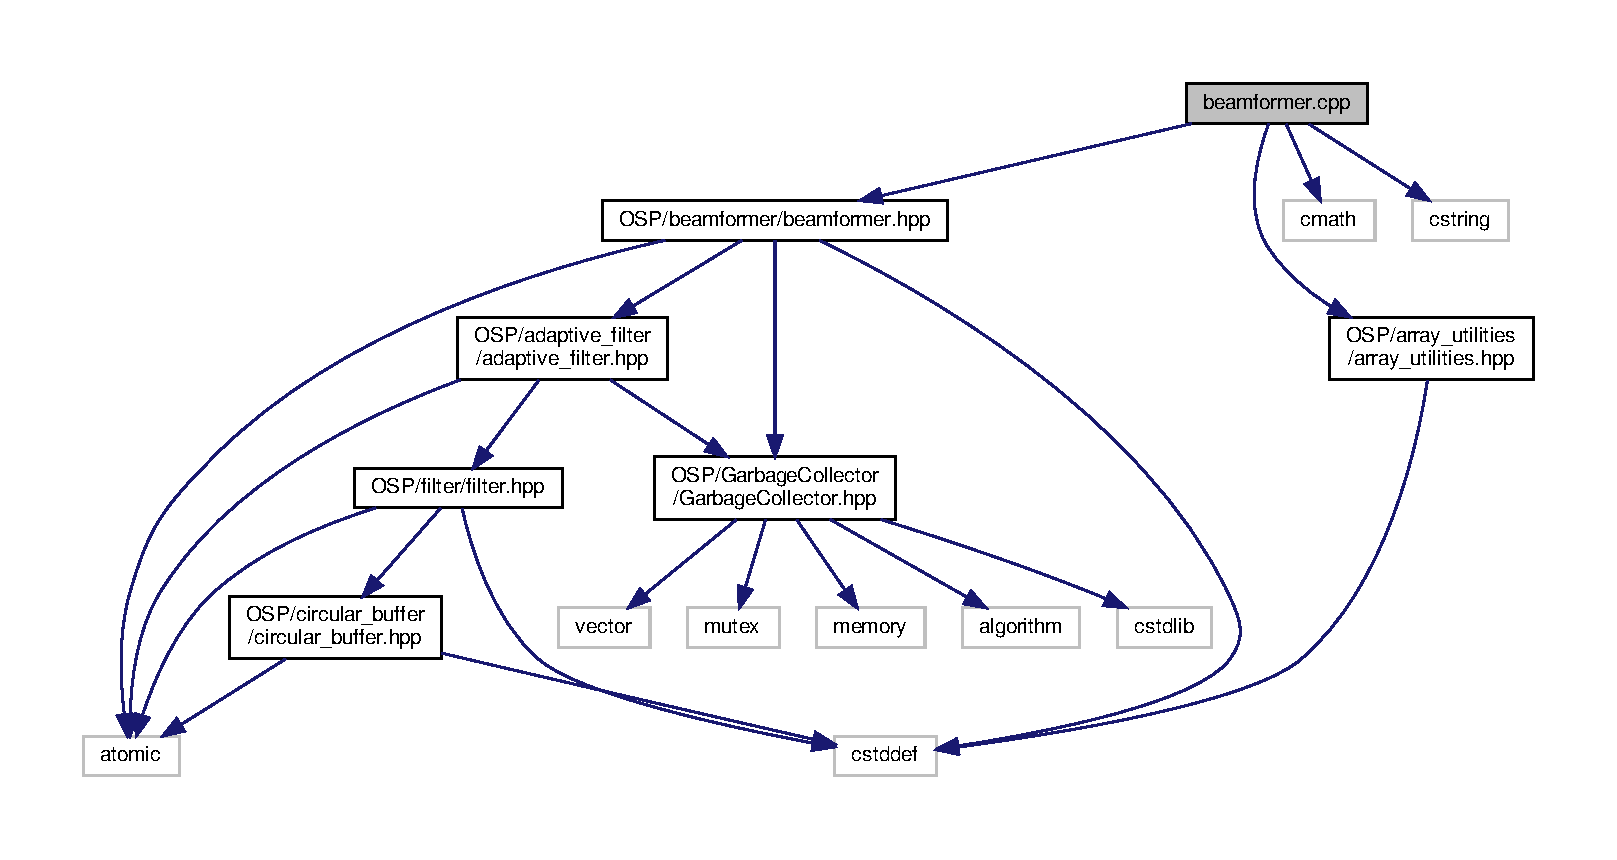
\includegraphics[width=350pt]{beamformer_8cpp__incl}
\end{center}
\end{figure}


\subsection{Detailed Description}
\begin{DoxyAuthor}{Author}
Open Speech Platform (O\+SP) Team, U\+C\+SD 
\end{DoxyAuthor}
\begin{DoxyCopyright}{Copyright}
Copyright (C) 2020 Regents of the University of California Redistribution and use in source and binary forms, with or without modification, are permitted provided that the following conditions are met\+: \begin{DoxyVerb}1. Redistributions of source code must retain the above copyright notice, this list of conditions and the
following disclaimer.

2. Redistributions in binary form must reproduce the above copyright notice, this list of conditions and the
following disclaimer in the documentation and/or other materials provided with the distribution.
\end{DoxyVerb}

\end{DoxyCopyright}
T\+H\+IS S\+O\+F\+T\+W\+A\+RE IS P\+R\+O\+V\+I\+D\+ED BY T\+HE C\+O\+P\+Y\+R\+I\+G\+HT H\+O\+L\+D\+E\+RS A\+ND C\+O\+N\+T\+R\+I\+B\+U\+T\+O\+RS \char`\"{}\+A\+S I\+S\char`\"{} A\+ND A\+NY E\+X\+P\+R\+E\+SS OR I\+M\+P\+L\+I\+ED W\+A\+R\+R\+A\+N\+T\+I\+ES, I\+N\+C\+L\+U\+D\+I\+NG, B\+UT N\+OT L\+I\+M\+I\+T\+ED TO, T\+HE I\+M\+P\+L\+I\+ED W\+A\+R\+R\+A\+N\+T\+I\+ES OF M\+E\+R\+C\+H\+A\+N\+T\+A\+B\+I\+L\+I\+TY A\+ND F\+I\+T\+N\+E\+SS F\+OR A P\+A\+R\+T\+I\+C\+U\+L\+AR P\+U\+R\+P\+O\+SE A\+RE D\+I\+S\+C\+L\+A\+I\+M\+ED. IN NO E\+V\+E\+NT S\+H\+A\+LL T\+HE C\+O\+P\+Y\+R\+I\+G\+HT H\+O\+L\+D\+ER OR C\+O\+N\+T\+R\+I\+B\+U\+T\+O\+RS BE L\+I\+A\+B\+LE F\+OR A\+NY D\+I\+R\+E\+CT, I\+N\+D\+I\+R\+E\+CT, I\+N\+C\+I\+D\+E\+N\+T\+AL, S\+P\+E\+C\+I\+AL, E\+X\+E\+M\+P\+L\+A\+RY, OR C\+O\+N\+S\+E\+Q\+U\+E\+N\+T\+I\+AL D\+A\+M\+A\+G\+ES (I\+N\+C\+L\+U\+D\+I\+NG, B\+UT N\+OT L\+I\+M\+I\+T\+ED TO, P\+R\+O\+C\+U\+R\+E\+M\+E\+NT OF S\+U\+B\+S\+T\+I\+T\+U\+TE G\+O\+O\+DS OR S\+E\+R\+V\+I\+C\+ES; L\+O\+SS OF U\+SE, D\+A\+TA, OR P\+R\+O\+F\+I\+TS; OR B\+U\+S\+I\+N\+E\+SS I\+N\+T\+E\+R\+R\+U\+P\+T\+I\+ON) H\+O\+W\+E\+V\+ER C\+A\+U\+S\+ED A\+ND ON A\+NY T\+H\+E\+O\+RY OF L\+I\+A\+B\+I\+L\+I\+TY, W\+H\+E\+T\+H\+ER IN C\+O\+N\+T\+R\+A\+CT, S\+T\+R\+I\+CT L\+I\+A\+B\+I\+L\+I\+TY, OR T\+O\+RT (I\+N\+C\+L\+U\+D\+I\+NG N\+E\+G\+L\+I\+G\+E\+N\+CE OR O\+T\+H\+E\+R\+W\+I\+SE) A\+R\+I\+S\+I\+NG IN A\+NY W\+AY O\+UT OF T\+HE U\+SE OF T\+H\+IS S\+O\+F\+T\+W\+A\+RE, E\+V\+EN IF A\+D\+V\+I\+S\+ED OF T\+HE P\+O\+S\+S\+I\+B\+I\+L\+I\+TY OF S\+U\+CH D\+A\+M\+A\+GE. 
\hypertarget{beamformer_8hpp}{}\section{beamformer.\+hpp File Reference}
\label{beamformer_8hpp}\index{beamformer.\+hpp@{beamformer.\+hpp}}
{\ttfamily \#include $<$cstddef$>$}\newline
{\ttfamily \#include $<$O\+S\+P/adaptive\+\_\+filter/adaptive\+\_\+filter.\+hpp$>$}\newline
{\ttfamily \#include $<$atomic$>$}\newline
{\ttfamily \#include $<$O\+S\+P/\+Garbage\+Collector/\+Garbage\+Collector.\+hpp$>$}\newline
Include dependency graph for beamformer.\+hpp\+:\nopagebreak
\begin{figure}[H]
\begin{center}
\leavevmode
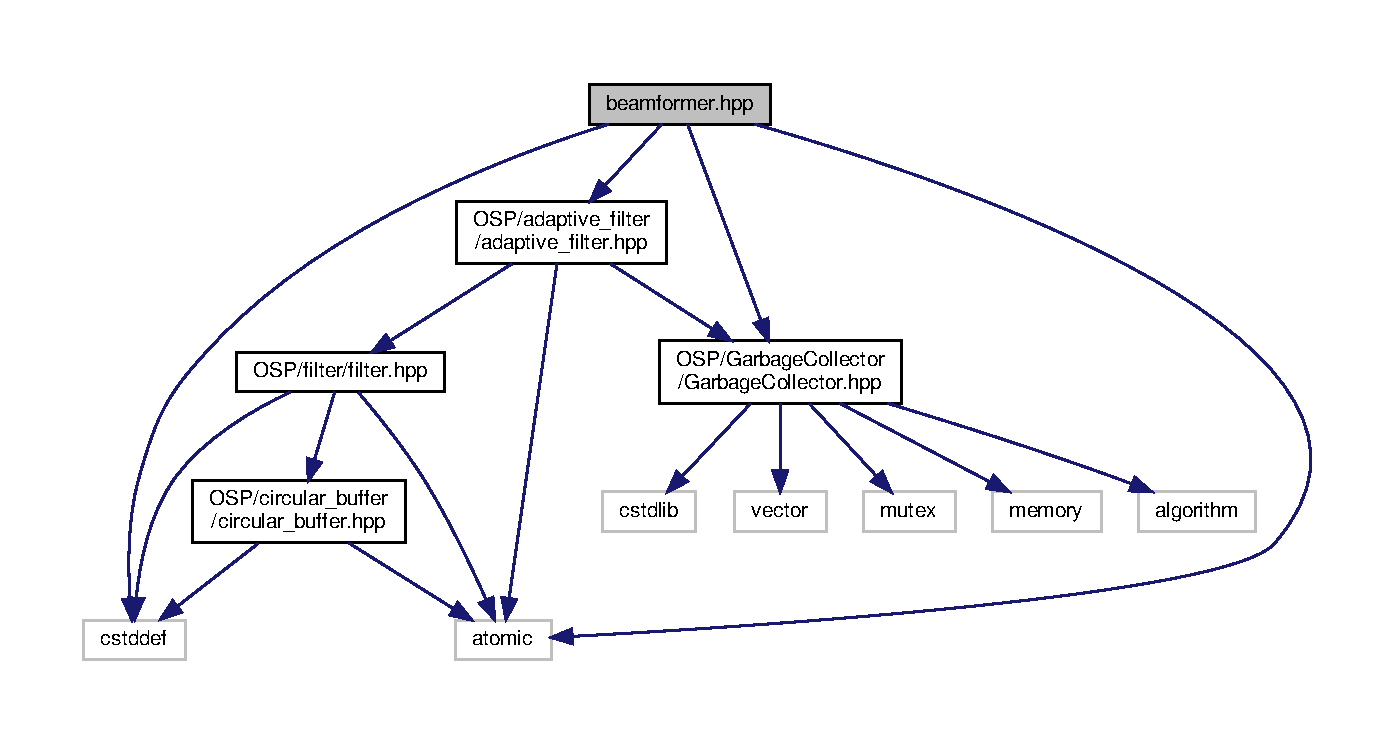
\includegraphics[width=350pt]{beamformer_8hpp__incl}
\end{center}
\end{figure}
This graph shows which files directly or indirectly include this file\+:\nopagebreak
\begin{figure}[H]
\begin{center}
\leavevmode
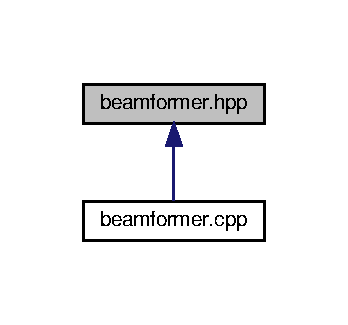
\includegraphics[width=167pt]{beamformer_8hpp__dep__incl}
\end{center}
\end{figure}
\subsection*{Classes}
\begin{DoxyCompactItemize}
\item 
class \hyperlink{classbeamformer}{beamformer}
\begin{DoxyCompactList}\small\item\em Beamformer Class. \end{DoxyCompactList}\end{DoxyCompactItemize}


\subsection{Detailed Description}
\begin{DoxyAuthor}{Author}
Open Speech Platform (O\+SP) Team, U\+C\+SD 
\end{DoxyAuthor}
\begin{DoxyCopyright}{Copyright}
Copyright (C) 2020 Regents of the University of California Redistribution and use in source and binary forms, with or without modification, are permitted provided that the following conditions are met\+: \begin{DoxyVerb}1. Redistributions of source code must retain the above copyright notice, this list of conditions and the
following disclaimer.

2. Redistributions in binary form must reproduce the above copyright notice, this list of conditions and the
following disclaimer in the documentation and/or other materials provided with the distribution.
\end{DoxyVerb}

\end{DoxyCopyright}
T\+H\+IS S\+O\+F\+T\+W\+A\+RE IS P\+R\+O\+V\+I\+D\+ED BY T\+HE C\+O\+P\+Y\+R\+I\+G\+HT H\+O\+L\+D\+E\+RS A\+ND C\+O\+N\+T\+R\+I\+B\+U\+T\+O\+RS \char`\"{}\+A\+S I\+S\char`\"{} A\+ND A\+NY E\+X\+P\+R\+E\+SS OR I\+M\+P\+L\+I\+ED W\+A\+R\+R\+A\+N\+T\+I\+ES, I\+N\+C\+L\+U\+D\+I\+NG, B\+UT N\+OT L\+I\+M\+I\+T\+ED TO, T\+HE I\+M\+P\+L\+I\+ED W\+A\+R\+R\+A\+N\+T\+I\+ES OF M\+E\+R\+C\+H\+A\+N\+T\+A\+B\+I\+L\+I\+TY A\+ND F\+I\+T\+N\+E\+SS F\+OR A P\+A\+R\+T\+I\+C\+U\+L\+AR P\+U\+R\+P\+O\+SE A\+RE D\+I\+S\+C\+L\+A\+I\+M\+ED. IN NO E\+V\+E\+NT S\+H\+A\+LL T\+HE C\+O\+P\+Y\+R\+I\+G\+HT H\+O\+L\+D\+ER OR C\+O\+N\+T\+R\+I\+B\+U\+T\+O\+RS BE L\+I\+A\+B\+LE F\+OR A\+NY D\+I\+R\+E\+CT, I\+N\+D\+I\+R\+E\+CT, I\+N\+C\+I\+D\+E\+N\+T\+AL, S\+P\+E\+C\+I\+AL, E\+X\+E\+M\+P\+L\+A\+RY, OR C\+O\+N\+S\+E\+Q\+U\+E\+N\+T\+I\+AL D\+A\+M\+A\+G\+ES (I\+N\+C\+L\+U\+D\+I\+NG, B\+UT N\+OT L\+I\+M\+I\+T\+ED TO, P\+R\+O\+C\+U\+R\+E\+M\+E\+NT OF S\+U\+B\+S\+T\+I\+T\+U\+TE G\+O\+O\+DS OR S\+E\+R\+V\+I\+C\+ES; L\+O\+SS OF U\+SE, D\+A\+TA, OR P\+R\+O\+F\+I\+TS; OR B\+U\+S\+I\+N\+E\+SS I\+N\+T\+E\+R\+R\+U\+P\+T\+I\+ON) H\+O\+W\+E\+V\+ER C\+A\+U\+S\+ED A\+ND ON A\+NY T\+H\+E\+O\+RY OF L\+I\+A\+B\+I\+L\+I\+TY, W\+H\+E\+T\+H\+ER IN C\+O\+N\+T\+R\+A\+CT, S\+T\+R\+I\+CT L\+I\+A\+B\+I\+L\+I\+TY, OR T\+O\+RT (I\+N\+C\+L\+U\+D\+I\+NG N\+E\+G\+L\+I\+G\+E\+N\+CE OR O\+T\+H\+E\+R\+W\+I\+SE) A\+R\+I\+S\+I\+NG IN A\+NY W\+AY O\+UT OF T\+HE U\+SE OF T\+H\+IS S\+O\+F\+T\+W\+A\+RE, E\+V\+EN IF A\+D\+V\+I\+S\+ED OF T\+HE P\+O\+S\+S\+I\+B\+I\+L\+I\+TY OF S\+U\+CH D\+A\+M\+A\+GE. 
\hypertarget{circular__buffer_8cpp}{}\section{circular\+\_\+buffer.\+cpp File Reference}
\label{circular__buffer_8cpp}\index{circular\+\_\+buffer.\+cpp@{circular\+\_\+buffer.\+cpp}}
{\ttfamily \#include $<$memory$>$}\newline
{\ttfamily \#include $<$cmath$>$}\newline
{\ttfamily \#include $<$cstring$>$}\newline
{\ttfamily \#include $<$shared\+\_\+mutex$>$}\newline
{\ttfamily \#include $<$O\+S\+P/circular\+\_\+buffer/circular\+\_\+buffer.\+hpp$>$}\newline
Include dependency graph for circular\+\_\+buffer.\+cpp\+:\nopagebreak
\begin{figure}[H]
\begin{center}
\leavevmode
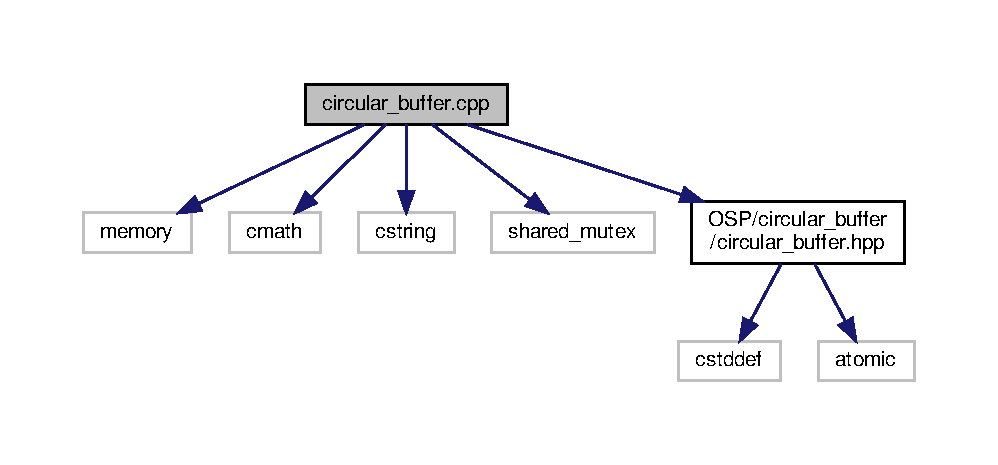
\includegraphics[width=350pt]{circular__buffer_8cpp__incl}
\end{center}
\end{figure}


\subsection{Detailed Description}
\begin{DoxyAuthor}{Author}
Open Speech Platform (O\+SP) Team, U\+C\+SD 
\end{DoxyAuthor}
\begin{DoxyCopyright}{Copyright}
Copyright (C) 2020 Regents of the University of California Redistribution and use in source and binary forms, with or without modification, are permitted provided that the following conditions are met\+: \begin{DoxyVerb}1. Redistributions of source code must retain the above copyright notice, this list of conditions and the
following disclaimer.

2. Redistributions in binary form must reproduce the above copyright notice, this list of conditions and the
following disclaimer in the documentation and/or other materials provided with the distribution.
\end{DoxyVerb}

\end{DoxyCopyright}
T\+H\+IS S\+O\+F\+T\+W\+A\+RE IS P\+R\+O\+V\+I\+D\+ED BY T\+HE C\+O\+P\+Y\+R\+I\+G\+HT H\+O\+L\+D\+E\+RS A\+ND C\+O\+N\+T\+R\+I\+B\+U\+T\+O\+RS \char`\"{}\+A\+S I\+S\char`\"{} A\+ND A\+NY E\+X\+P\+R\+E\+SS OR I\+M\+P\+L\+I\+ED W\+A\+R\+R\+A\+N\+T\+I\+ES, I\+N\+C\+L\+U\+D\+I\+NG, B\+UT N\+OT L\+I\+M\+I\+T\+ED TO, T\+HE I\+M\+P\+L\+I\+ED W\+A\+R\+R\+A\+N\+T\+I\+ES OF M\+E\+R\+C\+H\+A\+N\+T\+A\+B\+I\+L\+I\+TY A\+ND F\+I\+T\+N\+E\+SS F\+OR A P\+A\+R\+T\+I\+C\+U\+L\+AR P\+U\+R\+P\+O\+SE A\+RE D\+I\+S\+C\+L\+A\+I\+M\+ED. IN NO E\+V\+E\+NT S\+H\+A\+LL T\+HE C\+O\+P\+Y\+R\+I\+G\+HT H\+O\+L\+D\+ER OR C\+O\+N\+T\+R\+I\+B\+U\+T\+O\+RS BE L\+I\+A\+B\+LE F\+OR A\+NY D\+I\+R\+E\+CT, I\+N\+D\+I\+R\+E\+CT, I\+N\+C\+I\+D\+E\+N\+T\+AL, S\+P\+E\+C\+I\+AL, E\+X\+E\+M\+P\+L\+A\+RY, OR C\+O\+N\+S\+E\+Q\+U\+E\+N\+T\+I\+AL D\+A\+M\+A\+G\+ES (I\+N\+C\+L\+U\+D\+I\+NG, B\+UT N\+OT L\+I\+M\+I\+T\+ED TO, P\+R\+O\+C\+U\+R\+E\+M\+E\+NT OF S\+U\+B\+S\+T\+I\+T\+U\+TE G\+O\+O\+DS OR S\+E\+R\+V\+I\+C\+ES; L\+O\+SS OF U\+SE, D\+A\+TA, OR P\+R\+O\+F\+I\+TS; OR B\+U\+S\+I\+N\+E\+SS I\+N\+T\+E\+R\+R\+U\+P\+T\+I\+ON) H\+O\+W\+E\+V\+ER C\+A\+U\+S\+ED A\+ND ON A\+NY T\+H\+E\+O\+RY OF L\+I\+A\+B\+I\+L\+I\+TY, W\+H\+E\+T\+H\+ER IN C\+O\+N\+T\+R\+A\+CT, S\+T\+R\+I\+CT L\+I\+A\+B\+I\+L\+I\+TY, OR T\+O\+RT (I\+N\+C\+L\+U\+D\+I\+NG N\+E\+G\+L\+I\+G\+E\+N\+CE OR O\+T\+H\+E\+R\+W\+I\+SE) A\+R\+I\+S\+I\+NG IN A\+NY W\+AY O\+UT OF T\+HE U\+SE OF T\+H\+IS S\+O\+F\+T\+W\+A\+RE, E\+V\+EN IF A\+D\+V\+I\+S\+ED OF T\+HE P\+O\+S\+S\+I\+B\+I\+L\+I\+TY OF S\+U\+CH D\+A\+M\+A\+GE. 
\hypertarget{circular__buffer_8hpp}{}\section{circular\+\_\+buffer.\+hpp File Reference}
\label{circular__buffer_8hpp}\index{circular\+\_\+buffer.\+hpp@{circular\+\_\+buffer.\+hpp}}
{\ttfamily \#include $<$cstddef$>$}\newline
{\ttfamily \#include $<$atomic$>$}\newline
Include dependency graph for circular\+\_\+buffer.\+hpp\+:\nopagebreak
\begin{figure}[H]
\begin{center}
\leavevmode
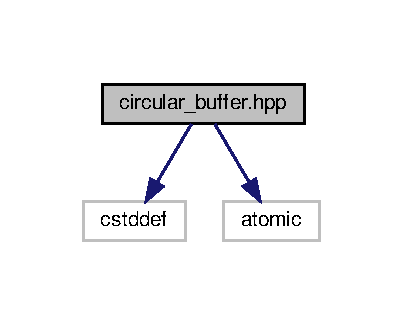
\includegraphics[width=194pt]{circular__buffer_8hpp__incl}
\end{center}
\end{figure}
This graph shows which files directly or indirectly include this file\+:\nopagebreak
\begin{figure}[H]
\begin{center}
\leavevmode
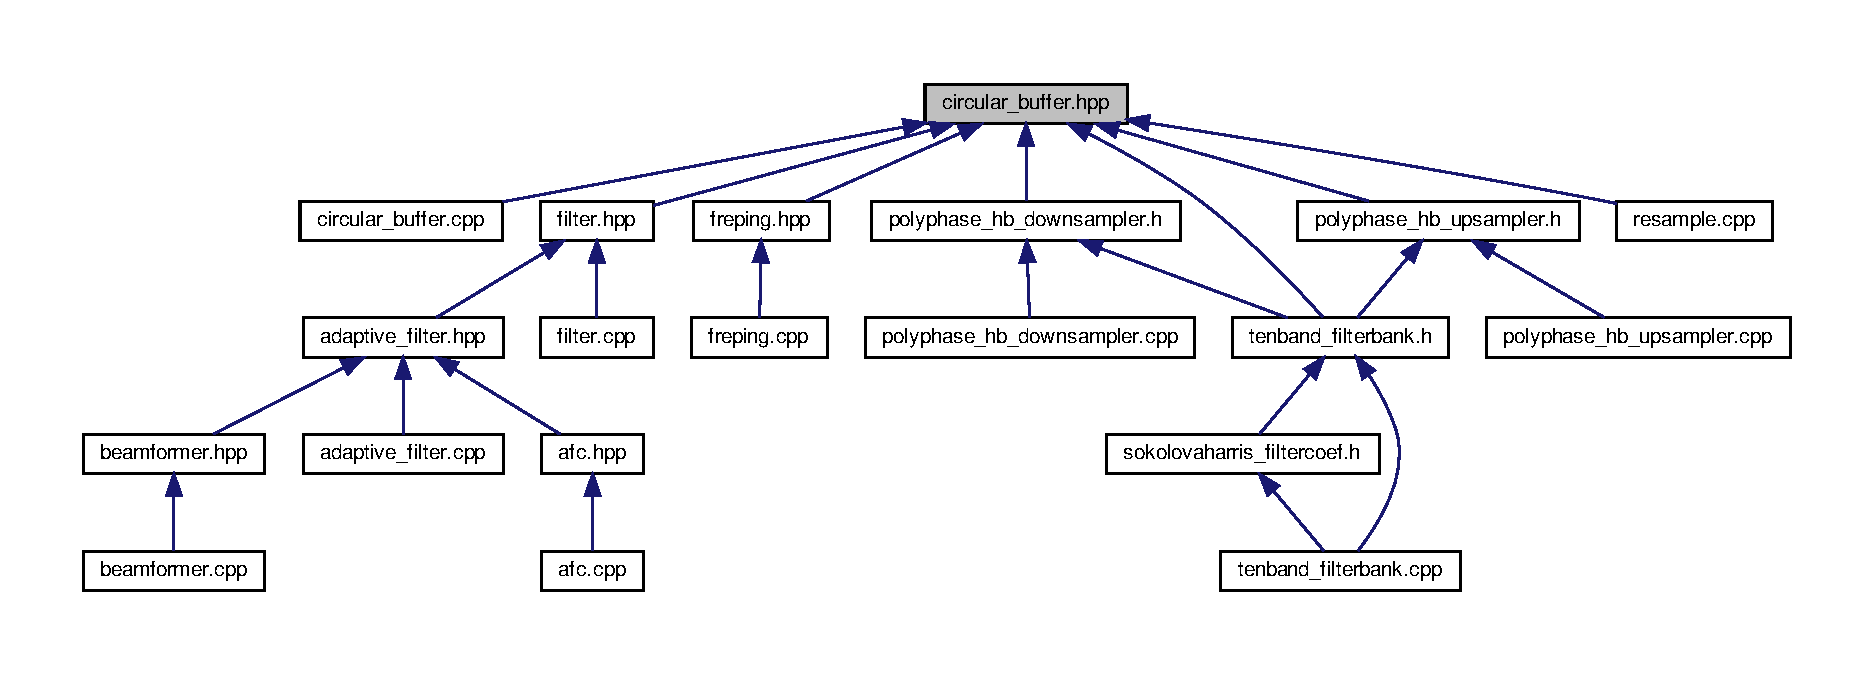
\includegraphics[width=350pt]{circular__buffer_8hpp__dep__incl}
\end{center}
\end{figure}
\subsection*{Classes}
\begin{DoxyCompactItemize}
\item 
class \hyperlink{classcircular__buffer}{circular\+\_\+buffer}
\begin{DoxyCompactList}\small\item\em Circular Buffer Class. \end{DoxyCompactList}\end{DoxyCompactItemize}


\subsection{Detailed Description}
\begin{DoxyAuthor}{Author}
Open Speech Platform (O\+SP) Team, U\+C\+SD 
\end{DoxyAuthor}
\begin{DoxyCopyright}{Copyright}
Copyright (C) 2020 Regents of the University of California Redistribution and use in source and binary forms, with or without modification, are permitted provided that the following conditions are met\+: \begin{DoxyVerb}1. Redistributions of source code must retain the above copyright notice, this list of conditions and the
following disclaimer.

2. Redistributions in binary form must reproduce the above copyright notice, this list of conditions and the
following disclaimer in the documentation and/or other materials provided with the distribution.
\end{DoxyVerb}

\end{DoxyCopyright}
T\+H\+IS S\+O\+F\+T\+W\+A\+RE IS P\+R\+O\+V\+I\+D\+ED BY T\+HE C\+O\+P\+Y\+R\+I\+G\+HT H\+O\+L\+D\+E\+RS A\+ND C\+O\+N\+T\+R\+I\+B\+U\+T\+O\+RS \char`\"{}\+A\+S I\+S\char`\"{} A\+ND A\+NY E\+X\+P\+R\+E\+SS OR I\+M\+P\+L\+I\+ED W\+A\+R\+R\+A\+N\+T\+I\+ES, I\+N\+C\+L\+U\+D\+I\+NG, B\+UT N\+OT L\+I\+M\+I\+T\+ED TO, T\+HE I\+M\+P\+L\+I\+ED W\+A\+R\+R\+A\+N\+T\+I\+ES OF M\+E\+R\+C\+H\+A\+N\+T\+A\+B\+I\+L\+I\+TY A\+ND F\+I\+T\+N\+E\+SS F\+OR A P\+A\+R\+T\+I\+C\+U\+L\+AR P\+U\+R\+P\+O\+SE A\+RE D\+I\+S\+C\+L\+A\+I\+M\+ED. IN NO E\+V\+E\+NT S\+H\+A\+LL T\+HE C\+O\+P\+Y\+R\+I\+G\+HT H\+O\+L\+D\+ER OR C\+O\+N\+T\+R\+I\+B\+U\+T\+O\+RS BE L\+I\+A\+B\+LE F\+OR A\+NY D\+I\+R\+E\+CT, I\+N\+D\+I\+R\+E\+CT, I\+N\+C\+I\+D\+E\+N\+T\+AL, S\+P\+E\+C\+I\+AL, E\+X\+E\+M\+P\+L\+A\+RY, OR C\+O\+N\+S\+E\+Q\+U\+E\+N\+T\+I\+AL D\+A\+M\+A\+G\+ES (I\+N\+C\+L\+U\+D\+I\+NG, B\+UT N\+OT L\+I\+M\+I\+T\+ED TO, P\+R\+O\+C\+U\+R\+E\+M\+E\+NT OF S\+U\+B\+S\+T\+I\+T\+U\+TE G\+O\+O\+DS OR S\+E\+R\+V\+I\+C\+ES; L\+O\+SS OF U\+SE, D\+A\+TA, OR P\+R\+O\+F\+I\+TS; OR B\+U\+S\+I\+N\+E\+SS I\+N\+T\+E\+R\+R\+U\+P\+T\+I\+ON) H\+O\+W\+E\+V\+ER C\+A\+U\+S\+ED A\+ND ON A\+NY T\+H\+E\+O\+RY OF L\+I\+A\+B\+I\+L\+I\+TY, W\+H\+E\+T\+H\+ER IN C\+O\+N\+T\+R\+A\+CT, S\+T\+R\+I\+CT L\+I\+A\+B\+I\+L\+I\+TY, OR T\+O\+RT (I\+N\+C\+L\+U\+D\+I\+NG N\+E\+G\+L\+I\+G\+E\+N\+CE OR O\+T\+H\+E\+R\+W\+I\+SE) A\+R\+I\+S\+I\+NG IN A\+NY W\+AY O\+UT OF T\+HE U\+SE OF T\+H\+IS S\+O\+F\+T\+W\+A\+RE, E\+V\+EN IF A\+D\+V\+I\+S\+ED OF T\+HE P\+O\+S\+S\+I\+B\+I\+L\+I\+TY OF S\+U\+CH D\+A\+M\+A\+GE. 
\hypertarget{filter_8cpp}{}\section{filter.\+cpp File Reference}
\label{filter_8cpp}\index{filter.\+cpp@{filter.\+cpp}}
{\ttfamily \#include $<$memory$>$}\newline
{\ttfamily \#include $<$mutex$>$}\newline
{\ttfamily \#include $<$O\+S\+P/filter/filter.\+hpp$>$}\newline
Include dependency graph for filter.\+cpp\+:\nopagebreak
\begin{figure}[H]
\begin{center}
\leavevmode
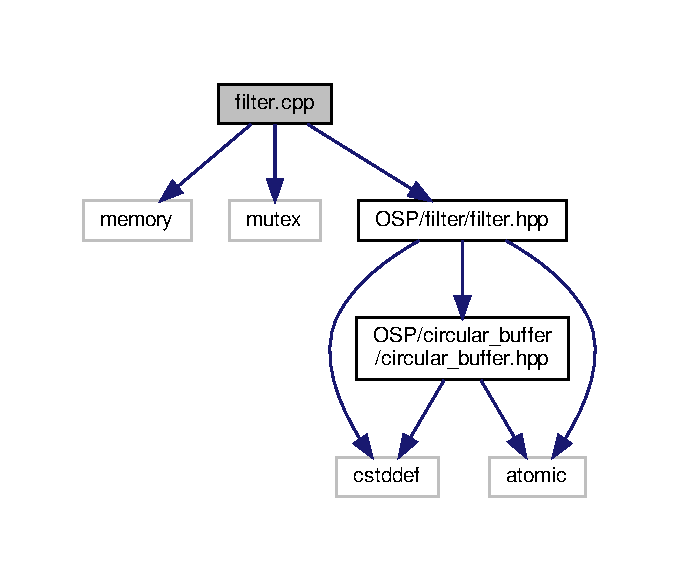
\includegraphics[width=326pt]{filter_8cpp__incl}
\end{center}
\end{figure}


\subsection{Detailed Description}
\begin{DoxyAuthor}{Author}
Open Speech Platform (O\+SP) Team, U\+C\+SD 
\end{DoxyAuthor}
\begin{DoxyCopyright}{Copyright}
Copyright (C) 2020 Regents of the University of California Redistribution and use in source and binary forms, with or without modification, are permitted provided that the following conditions are met\+: \begin{DoxyVerb}1. Redistributions of source code must retain the above copyright notice, this list of conditions and the
following disclaimer.

2. Redistributions in binary form must reproduce the above copyright notice, this list of conditions and the
following disclaimer in the documentation and/or other materials provided with the distribution.
\end{DoxyVerb}

\end{DoxyCopyright}
T\+H\+IS S\+O\+F\+T\+W\+A\+RE IS P\+R\+O\+V\+I\+D\+ED BY T\+HE C\+O\+P\+Y\+R\+I\+G\+HT H\+O\+L\+D\+E\+RS A\+ND C\+O\+N\+T\+R\+I\+B\+U\+T\+O\+RS \char`\"{}\+A\+S I\+S\char`\"{} A\+ND A\+NY E\+X\+P\+R\+E\+SS OR I\+M\+P\+L\+I\+ED W\+A\+R\+R\+A\+N\+T\+I\+ES, I\+N\+C\+L\+U\+D\+I\+NG, B\+UT N\+OT L\+I\+M\+I\+T\+ED TO, T\+HE I\+M\+P\+L\+I\+ED W\+A\+R\+R\+A\+N\+T\+I\+ES OF M\+E\+R\+C\+H\+A\+N\+T\+A\+B\+I\+L\+I\+TY A\+ND F\+I\+T\+N\+E\+SS F\+OR A P\+A\+R\+T\+I\+C\+U\+L\+AR P\+U\+R\+P\+O\+SE A\+RE D\+I\+S\+C\+L\+A\+I\+M\+ED. IN NO E\+V\+E\+NT S\+H\+A\+LL T\+HE C\+O\+P\+Y\+R\+I\+G\+HT H\+O\+L\+D\+ER OR C\+O\+N\+T\+R\+I\+B\+U\+T\+O\+RS BE L\+I\+A\+B\+LE F\+OR A\+NY D\+I\+R\+E\+CT, I\+N\+D\+I\+R\+E\+CT, I\+N\+C\+I\+D\+E\+N\+T\+AL, S\+P\+E\+C\+I\+AL, E\+X\+E\+M\+P\+L\+A\+RY, OR C\+O\+N\+S\+E\+Q\+U\+E\+N\+T\+I\+AL D\+A\+M\+A\+G\+ES (I\+N\+C\+L\+U\+D\+I\+NG, B\+UT N\+OT L\+I\+M\+I\+T\+ED TO, P\+R\+O\+C\+U\+R\+E\+M\+E\+NT OF S\+U\+B\+S\+T\+I\+T\+U\+TE G\+O\+O\+DS OR S\+E\+R\+V\+I\+C\+ES; L\+O\+SS OF U\+SE, D\+A\+TA, OR P\+R\+O\+F\+I\+TS; OR B\+U\+S\+I\+N\+E\+SS I\+N\+T\+E\+R\+R\+U\+P\+T\+I\+ON) H\+O\+W\+E\+V\+ER C\+A\+U\+S\+ED A\+ND ON A\+NY T\+H\+E\+O\+RY OF L\+I\+A\+B\+I\+L\+I\+TY, W\+H\+E\+T\+H\+ER IN C\+O\+N\+T\+R\+A\+CT, S\+T\+R\+I\+CT L\+I\+A\+B\+I\+L\+I\+TY, OR T\+O\+RT (I\+N\+C\+L\+U\+D\+I\+NG N\+E\+G\+L\+I\+G\+E\+N\+CE OR O\+T\+H\+E\+R\+W\+I\+SE) A\+R\+I\+S\+I\+NG IN A\+NY W\+AY O\+UT OF T\+HE U\+SE OF T\+H\+IS S\+O\+F\+T\+W\+A\+RE, E\+V\+EN IF A\+D\+V\+I\+S\+ED OF T\+HE P\+O\+S\+S\+I\+B\+I\+L\+I\+TY OF S\+U\+CH D\+A\+M\+A\+GE. 
\hypertarget{filter_8hpp}{}\section{filter.\+hpp File Reference}
\label{filter_8hpp}\index{filter.\+hpp@{filter.\+hpp}}
{\ttfamily \#include $<$cstddef$>$}\newline
{\ttfamily \#include $<$atomic$>$}\newline
{\ttfamily \#include $<$O\+S\+P/circular\+\_\+buffer/circular\+\_\+buffer.\+hpp$>$}\newline
Include dependency graph for filter.\+hpp\+:\nopagebreak
\begin{figure}[H]
\begin{center}
\leavevmode
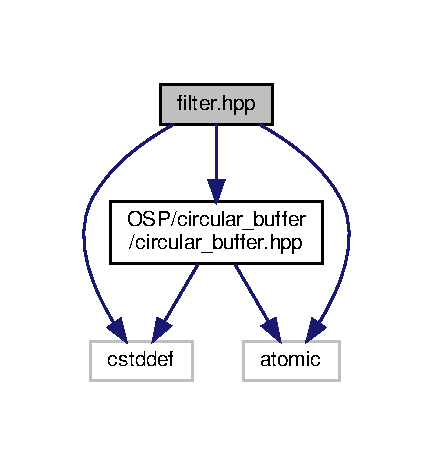
\includegraphics[width=208pt]{filter_8hpp__incl}
\end{center}
\end{figure}
This graph shows which files directly or indirectly include this file\+:\nopagebreak
\begin{figure}[H]
\begin{center}
\leavevmode
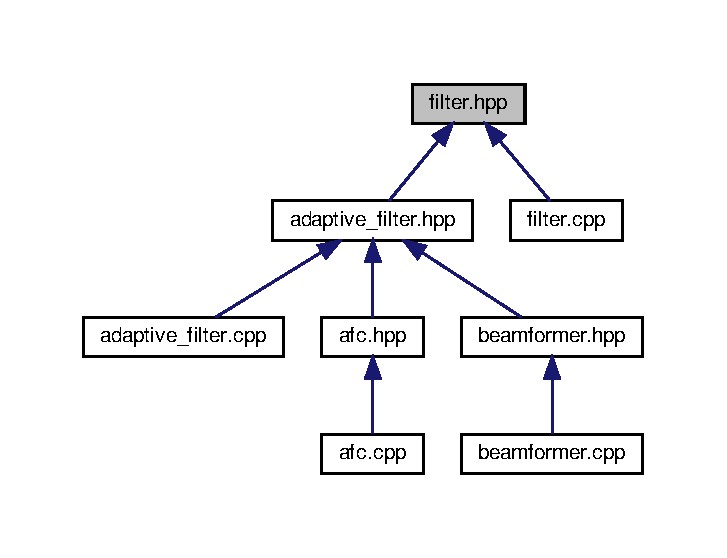
\includegraphics[width=349pt]{filter_8hpp__dep__incl}
\end{center}
\end{figure}
\subsection*{Classes}
\begin{DoxyCompactItemize}
\item 
class \hyperlink{classfilter}{filter}
\begin{DoxyCompactList}\small\item\em Filter Class. \end{DoxyCompactList}\end{DoxyCompactItemize}


\subsection{Detailed Description}
\begin{DoxyAuthor}{Author}
Open Speech Platform (O\+SP) Team, U\+C\+SD 
\end{DoxyAuthor}
\begin{DoxyCopyright}{Copyright}
Copyright (C) 2020 Regents of the University of California Redistribution and use in source and binary forms, with or without modification, are permitted provided that the following conditions are met\+: \begin{DoxyVerb}1. Redistributions of source code must retain the above copyright notice, this list of conditions and the
following disclaimer.

2. Redistributions in binary form must reproduce the above copyright notice, this list of conditions and the
following disclaimer in the documentation and/or other materials provided with the distribution.
\end{DoxyVerb}

\end{DoxyCopyright}
T\+H\+IS S\+O\+F\+T\+W\+A\+RE IS P\+R\+O\+V\+I\+D\+ED BY T\+HE C\+O\+P\+Y\+R\+I\+G\+HT H\+O\+L\+D\+E\+RS A\+ND C\+O\+N\+T\+R\+I\+B\+U\+T\+O\+RS \char`\"{}\+A\+S I\+S\char`\"{} A\+ND A\+NY E\+X\+P\+R\+E\+SS OR I\+M\+P\+L\+I\+ED W\+A\+R\+R\+A\+N\+T\+I\+ES, I\+N\+C\+L\+U\+D\+I\+NG, B\+UT N\+OT L\+I\+M\+I\+T\+ED TO, T\+HE I\+M\+P\+L\+I\+ED W\+A\+R\+R\+A\+N\+T\+I\+ES OF M\+E\+R\+C\+H\+A\+N\+T\+A\+B\+I\+L\+I\+TY A\+ND F\+I\+T\+N\+E\+SS F\+OR A P\+A\+R\+T\+I\+C\+U\+L\+AR P\+U\+R\+P\+O\+SE A\+RE D\+I\+S\+C\+L\+A\+I\+M\+ED. IN NO E\+V\+E\+NT S\+H\+A\+LL T\+HE C\+O\+P\+Y\+R\+I\+G\+HT H\+O\+L\+D\+ER OR C\+O\+N\+T\+R\+I\+B\+U\+T\+O\+RS BE L\+I\+A\+B\+LE F\+OR A\+NY D\+I\+R\+E\+CT, I\+N\+D\+I\+R\+E\+CT, I\+N\+C\+I\+D\+E\+N\+T\+AL, S\+P\+E\+C\+I\+AL, E\+X\+E\+M\+P\+L\+A\+RY, OR C\+O\+N\+S\+E\+Q\+U\+E\+N\+T\+I\+AL D\+A\+M\+A\+G\+ES (I\+N\+C\+L\+U\+D\+I\+NG, B\+UT N\+OT L\+I\+M\+I\+T\+ED TO, P\+R\+O\+C\+U\+R\+E\+M\+E\+NT OF S\+U\+B\+S\+T\+I\+T\+U\+TE G\+O\+O\+DS OR S\+E\+R\+V\+I\+C\+ES; L\+O\+SS OF U\+SE, D\+A\+TA, OR P\+R\+O\+F\+I\+TS; OR B\+U\+S\+I\+N\+E\+SS I\+N\+T\+E\+R\+R\+U\+P\+T\+I\+ON) H\+O\+W\+E\+V\+ER C\+A\+U\+S\+ED A\+ND ON A\+NY T\+H\+E\+O\+RY OF L\+I\+A\+B\+I\+L\+I\+TY, W\+H\+E\+T\+H\+ER IN C\+O\+N\+T\+R\+A\+CT, S\+T\+R\+I\+CT L\+I\+A\+B\+I\+L\+I\+TY, OR T\+O\+RT (I\+N\+C\+L\+U\+D\+I\+NG N\+E\+G\+L\+I\+G\+E\+N\+CE OR O\+T\+H\+E\+R\+W\+I\+SE) A\+R\+I\+S\+I\+NG IN A\+NY W\+AY O\+UT OF T\+HE U\+SE OF T\+H\+IS S\+O\+F\+T\+W\+A\+RE, E\+V\+EN IF A\+D\+V\+I\+S\+ED OF T\+HE P\+O\+S\+S\+I\+B\+I\+L\+I\+TY OF S\+U\+CH D\+A\+M\+A\+GE. 
\hypertarget{fir__formii_8cpp}{}\section{fir\+\_\+formii.\+cpp File Reference}
\label{fir__formii_8cpp}\index{fir\+\_\+formii.\+cpp@{fir\+\_\+formii.\+cpp}}
{\ttfamily \#include \char`\"{}fir\+\_\+formii.\+h\char`\"{}}\newline
Include dependency graph for fir\+\_\+formii.\+cpp\+:\nopagebreak
\begin{figure}[H]
\begin{center}
\leavevmode
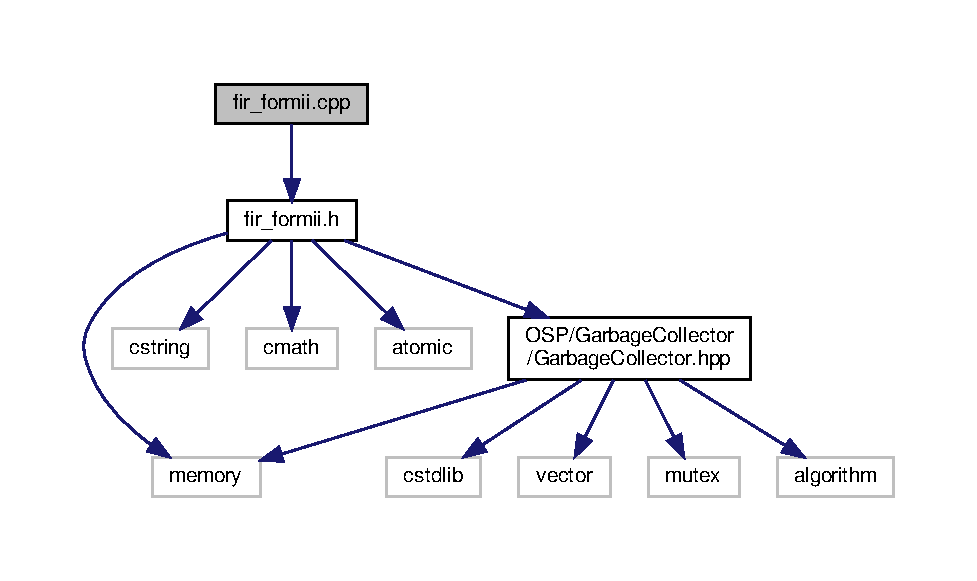
\includegraphics[width=350pt]{fir__formii_8cpp__incl}
\end{center}
\end{figure}


\subsection{Detailed Description}
\begin{DoxyAuthor}{Author}
Open Speech Platform (O\+SP) Team, U\+C\+SD 
\end{DoxyAuthor}
\begin{DoxyCopyright}{Copyright}
Copyright (C) 2020 Regents of the University of California Redistribution and use in source and binary forms, with or without modification, are permitted provided that the following conditions are met\+: \begin{DoxyVerb}1. Redistributions of source code must retain the above copyright notice, this list of conditions and the
following disclaimer.

2. Redistributions in binary form must reproduce the above copyright notice, this list of conditions and the
following disclaimer in the documentation and/or other materials provided with the distribution.
\end{DoxyVerb}

\end{DoxyCopyright}
T\+H\+IS S\+O\+F\+T\+W\+A\+RE IS P\+R\+O\+V\+I\+D\+ED BY T\+HE C\+O\+P\+Y\+R\+I\+G\+HT H\+O\+L\+D\+E\+RS A\+ND C\+O\+N\+T\+R\+I\+B\+U\+T\+O\+RS \char`\"{}\+A\+S I\+S\char`\"{} A\+ND A\+NY E\+X\+P\+R\+E\+SS OR I\+M\+P\+L\+I\+ED W\+A\+R\+R\+A\+N\+T\+I\+ES, I\+N\+C\+L\+U\+D\+I\+NG, B\+UT N\+OT L\+I\+M\+I\+T\+ED TO, T\+HE I\+M\+P\+L\+I\+ED W\+A\+R\+R\+A\+N\+T\+I\+ES OF M\+E\+R\+C\+H\+A\+N\+T\+A\+B\+I\+L\+I\+TY A\+ND F\+I\+T\+N\+E\+SS F\+OR A P\+A\+R\+T\+I\+C\+U\+L\+AR P\+U\+R\+P\+O\+SE A\+RE D\+I\+S\+C\+L\+A\+I\+M\+ED. IN NO E\+V\+E\+NT S\+H\+A\+LL T\+HE C\+O\+P\+Y\+R\+I\+G\+HT H\+O\+L\+D\+ER OR C\+O\+N\+T\+R\+I\+B\+U\+T\+O\+RS BE L\+I\+A\+B\+LE F\+OR A\+NY D\+I\+R\+E\+CT, I\+N\+D\+I\+R\+E\+CT, I\+N\+C\+I\+D\+E\+N\+T\+AL, S\+P\+E\+C\+I\+AL, E\+X\+E\+M\+P\+L\+A\+RY, OR C\+O\+N\+S\+E\+Q\+U\+E\+N\+T\+I\+AL D\+A\+M\+A\+G\+ES (I\+N\+C\+L\+U\+D\+I\+NG, B\+UT N\+OT L\+I\+M\+I\+T\+ED TO, P\+R\+O\+C\+U\+R\+E\+M\+E\+NT OF S\+U\+B\+S\+T\+I\+T\+U\+TE G\+O\+O\+DS OR S\+E\+R\+V\+I\+C\+ES; L\+O\+SS OF U\+SE, D\+A\+TA, OR P\+R\+O\+F\+I\+TS; OR B\+U\+S\+I\+N\+E\+SS I\+N\+T\+E\+R\+R\+U\+P\+T\+I\+ON) H\+O\+W\+E\+V\+ER C\+A\+U\+S\+ED A\+ND ON A\+NY T\+H\+E\+O\+RY OF L\+I\+A\+B\+I\+L\+I\+TY, W\+H\+E\+T\+H\+ER IN C\+O\+N\+T\+R\+A\+CT, S\+T\+R\+I\+CT L\+I\+A\+B\+I\+L\+I\+TY, OR T\+O\+RT (I\+N\+C\+L\+U\+D\+I\+NG N\+E\+G\+L\+I\+G\+E\+N\+CE OR O\+T\+H\+E\+R\+W\+I\+SE) A\+R\+I\+S\+I\+NG IN A\+NY W\+AY O\+UT OF T\+HE U\+SE OF T\+H\+IS S\+O\+F\+T\+W\+A\+RE, E\+V\+EN IF A\+D\+V\+I\+S\+ED OF T\+HE P\+O\+S\+S\+I\+B\+I\+L\+I\+TY OF S\+U\+CH D\+A\+M\+A\+GE. 
\hypertarget{fir__formii_8h}{}\section{fir\+\_\+formii.\+h File Reference}
\label{fir__formii_8h}\index{fir\+\_\+formii.\+h@{fir\+\_\+formii.\+h}}
{\ttfamily \#include $<$memory$>$}\newline
{\ttfamily \#include $<$cstring$>$}\newline
{\ttfamily \#include $<$cmath$>$}\newline
{\ttfamily \#include $<$atomic$>$}\newline
{\ttfamily \#include $<$O\+S\+P/\+Garbage\+Collector/\+Garbage\+Collector.\+hpp$>$}\newline
Include dependency graph for fir\+\_\+formii.\+h\+:\nopagebreak
\begin{figure}[H]
\begin{center}
\leavevmode
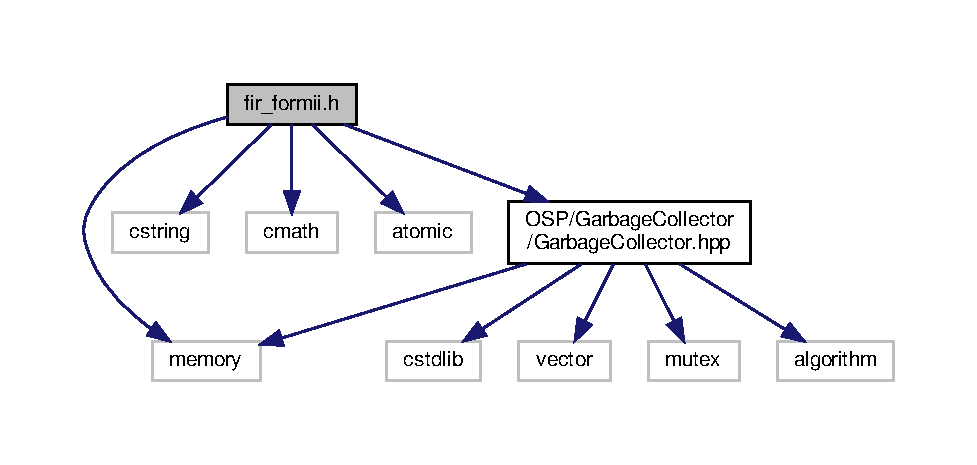
\includegraphics[width=350pt]{fir__formii_8h__incl}
\end{center}
\end{figure}
This graph shows which files directly or indirectly include this file\+:\nopagebreak
\begin{figure}[H]
\begin{center}
\leavevmode
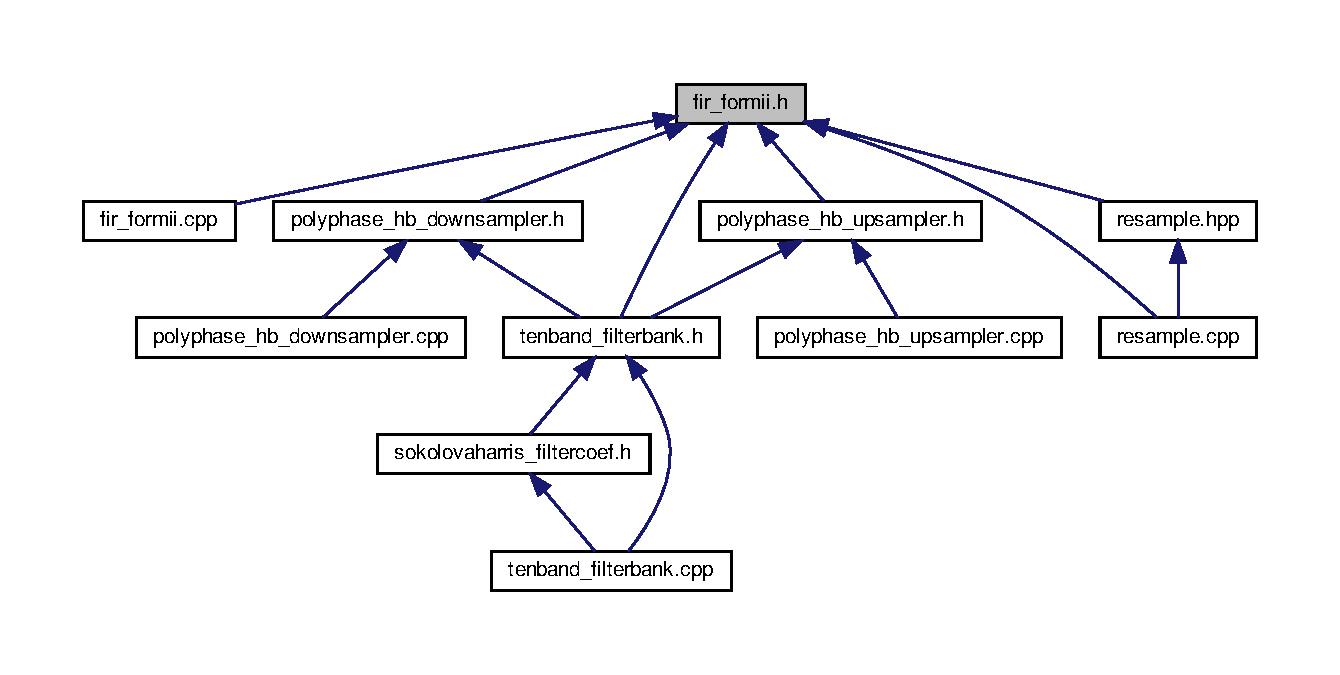
\includegraphics[width=350pt]{fir__formii_8h__dep__incl}
\end{center}
\end{figure}
\subsection*{Classes}
\begin{DoxyCompactItemize}
\item 
class \hyperlink{classfir__formii}{fir\+\_\+formii}
\begin{DoxyCompactList}\small\item\em Filter Class. \end{DoxyCompactList}\end{DoxyCompactItemize}


\subsection{Detailed Description}
\begin{DoxyAuthor}{Author}
Open Speech Platform (O\+SP) Team, U\+C\+SD 
\end{DoxyAuthor}
\begin{DoxyCopyright}{Copyright}
Copyright (C) 2020 Regents of the University of California Redistribution and use in source and binary forms, with or without modification, are permitted provided that the following conditions are met\+: \begin{DoxyVerb}1. Redistributions of source code must retain the above copyright notice, this list of conditions and the
following disclaimer.

2. Redistributions in binary form must reproduce the above copyright notice, this list of conditions and the
following disclaimer in the documentation and/or other materials provided with the distribution.
\end{DoxyVerb}

\end{DoxyCopyright}
T\+H\+IS S\+O\+F\+T\+W\+A\+RE IS P\+R\+O\+V\+I\+D\+ED BY T\+HE C\+O\+P\+Y\+R\+I\+G\+HT H\+O\+L\+D\+E\+RS A\+ND C\+O\+N\+T\+R\+I\+B\+U\+T\+O\+RS \char`\"{}\+A\+S I\+S\char`\"{} A\+ND A\+NY E\+X\+P\+R\+E\+SS OR I\+M\+P\+L\+I\+ED W\+A\+R\+R\+A\+N\+T\+I\+ES, I\+N\+C\+L\+U\+D\+I\+NG, B\+UT N\+OT L\+I\+M\+I\+T\+ED TO, T\+HE I\+M\+P\+L\+I\+ED W\+A\+R\+R\+A\+N\+T\+I\+ES OF M\+E\+R\+C\+H\+A\+N\+T\+A\+B\+I\+L\+I\+TY A\+ND F\+I\+T\+N\+E\+SS F\+OR A P\+A\+R\+T\+I\+C\+U\+L\+AR P\+U\+R\+P\+O\+SE A\+RE D\+I\+S\+C\+L\+A\+I\+M\+ED. IN NO E\+V\+E\+NT S\+H\+A\+LL T\+HE C\+O\+P\+Y\+R\+I\+G\+HT H\+O\+L\+D\+ER OR C\+O\+N\+T\+R\+I\+B\+U\+T\+O\+RS BE L\+I\+A\+B\+LE F\+OR A\+NY D\+I\+R\+E\+CT, I\+N\+D\+I\+R\+E\+CT, I\+N\+C\+I\+D\+E\+N\+T\+AL, S\+P\+E\+C\+I\+AL, E\+X\+E\+M\+P\+L\+A\+RY, OR C\+O\+N\+S\+E\+Q\+U\+E\+N\+T\+I\+AL D\+A\+M\+A\+G\+ES (I\+N\+C\+L\+U\+D\+I\+NG, B\+UT N\+OT L\+I\+M\+I\+T\+ED TO, P\+R\+O\+C\+U\+R\+E\+M\+E\+NT OF S\+U\+B\+S\+T\+I\+T\+U\+TE G\+O\+O\+DS OR S\+E\+R\+V\+I\+C\+ES; L\+O\+SS OF U\+SE, D\+A\+TA, OR P\+R\+O\+F\+I\+TS; OR B\+U\+S\+I\+N\+E\+SS I\+N\+T\+E\+R\+R\+U\+P\+T\+I\+ON) H\+O\+W\+E\+V\+ER C\+A\+U\+S\+ED A\+ND ON A\+NY T\+H\+E\+O\+RY OF L\+I\+A\+B\+I\+L\+I\+TY, W\+H\+E\+T\+H\+ER IN C\+O\+N\+T\+R\+A\+CT, S\+T\+R\+I\+CT L\+I\+A\+B\+I\+L\+I\+TY, OR T\+O\+RT (I\+N\+C\+L\+U\+D\+I\+NG N\+E\+G\+L\+I\+G\+E\+N\+CE OR O\+T\+H\+E\+R\+W\+I\+SE) A\+R\+I\+S\+I\+NG IN A\+NY W\+AY O\+UT OF T\+HE U\+SE OF T\+H\+IS S\+O\+F\+T\+W\+A\+RE, E\+V\+EN IF A\+D\+V\+I\+S\+ED OF T\+HE P\+O\+S\+S\+I\+B\+I\+L\+I\+TY OF S\+U\+CH D\+A\+M\+A\+GE. 
\hypertarget{freping_8cpp}{}\section{freping.\+cpp File Reference}
\label{freping_8cpp}\index{freping.\+cpp@{freping.\+cpp}}
{\ttfamily \#include $<$O\+S\+P/freping/freping.\+hpp$>$}\newline
Include dependency graph for freping.\+cpp\+:\nopagebreak
\begin{figure}[H]
\begin{center}
\leavevmode
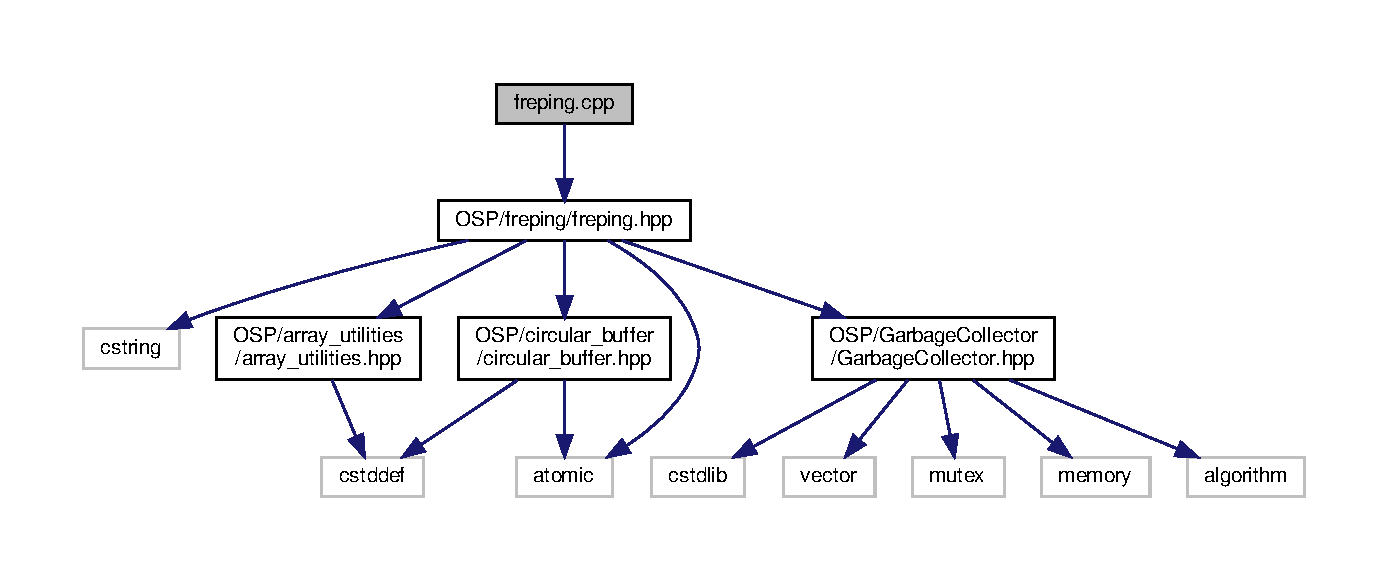
\includegraphics[width=350pt]{freping_8cpp__incl}
\end{center}
\end{figure}


\subsection{Detailed Description}
\begin{DoxyAuthor}{Author}
Open Speech Platform (O\+SP) Team, U\+C\+SD 
\end{DoxyAuthor}
\begin{DoxyCopyright}{Copyright}
Copyright (C) 2020 Regents of the University of California Redistribution and use in source and binary forms, with or without modification, are permitted provided that the following conditions are met\+: \begin{DoxyVerb}1. Redistributions of source code must retain the above copyright notice, this list of conditions and the
following disclaimer.

2. Redistributions in binary form must reproduce the above copyright notice, this list of conditions and the
following disclaimer in the documentation and/or other materials provided with the distribution.
\end{DoxyVerb}

\end{DoxyCopyright}
T\+H\+IS S\+O\+F\+T\+W\+A\+RE IS P\+R\+O\+V\+I\+D\+ED BY T\+HE C\+O\+P\+Y\+R\+I\+G\+HT H\+O\+L\+D\+E\+RS A\+ND C\+O\+N\+T\+R\+I\+B\+U\+T\+O\+RS \char`\"{}\+A\+S I\+S\char`\"{} A\+ND A\+NY E\+X\+P\+R\+E\+SS OR I\+M\+P\+L\+I\+ED W\+A\+R\+R\+A\+N\+T\+I\+ES, I\+N\+C\+L\+U\+D\+I\+NG, B\+UT N\+OT L\+I\+M\+I\+T\+ED TO, T\+HE I\+M\+P\+L\+I\+ED W\+A\+R\+R\+A\+N\+T\+I\+ES OF M\+E\+R\+C\+H\+A\+N\+T\+A\+B\+I\+L\+I\+TY A\+ND F\+I\+T\+N\+E\+SS F\+OR A P\+A\+R\+T\+I\+C\+U\+L\+AR P\+U\+R\+P\+O\+SE A\+RE D\+I\+S\+C\+L\+A\+I\+M\+ED. IN NO E\+V\+E\+NT S\+H\+A\+LL T\+HE C\+O\+P\+Y\+R\+I\+G\+HT H\+O\+L\+D\+ER OR C\+O\+N\+T\+R\+I\+B\+U\+T\+O\+RS BE L\+I\+A\+B\+LE F\+OR A\+NY D\+I\+R\+E\+CT, I\+N\+D\+I\+R\+E\+CT, I\+N\+C\+I\+D\+E\+N\+T\+AL, S\+P\+E\+C\+I\+AL, E\+X\+E\+M\+P\+L\+A\+RY, OR C\+O\+N\+S\+E\+Q\+U\+E\+N\+T\+I\+AL D\+A\+M\+A\+G\+ES (I\+N\+C\+L\+U\+D\+I\+NG, B\+UT N\+OT L\+I\+M\+I\+T\+ED TO, P\+R\+O\+C\+U\+R\+E\+M\+E\+NT OF S\+U\+B\+S\+T\+I\+T\+U\+TE G\+O\+O\+DS OR S\+E\+R\+V\+I\+C\+ES; L\+O\+SS OF U\+SE, D\+A\+TA, OR P\+R\+O\+F\+I\+TS; OR B\+U\+S\+I\+N\+E\+SS I\+N\+T\+E\+R\+R\+U\+P\+T\+I\+ON) H\+O\+W\+E\+V\+ER C\+A\+U\+S\+ED A\+ND ON A\+NY T\+H\+E\+O\+RY OF L\+I\+A\+B\+I\+L\+I\+TY, W\+H\+E\+T\+H\+ER IN C\+O\+N\+T\+R\+A\+CT, S\+T\+R\+I\+CT L\+I\+A\+B\+I\+L\+I\+TY, OR T\+O\+RT (I\+N\+C\+L\+U\+D\+I\+NG N\+E\+G\+L\+I\+G\+E\+N\+CE OR O\+T\+H\+E\+R\+W\+I\+SE) A\+R\+I\+S\+I\+NG IN A\+NY W\+AY O\+UT OF T\+HE U\+SE OF T\+H\+IS S\+O\+F\+T\+W\+A\+RE, E\+V\+EN IF A\+D\+V\+I\+S\+ED OF T\+HE P\+O\+S\+S\+I\+B\+I\+L\+I\+TY OF S\+U\+CH D\+A\+M\+A\+GE. 
\hypertarget{freping_8hpp}{}\section{freping.\+hpp File Reference}
\label{freping_8hpp}\index{freping.\+hpp@{freping.\+hpp}}
{\ttfamily \#include $<$cstring$>$}\newline
{\ttfamily \#include $<$O\+S\+P/circular\+\_\+buffer/circular\+\_\+buffer.\+hpp$>$}\newline
{\ttfamily \#include $<$O\+S\+P/array\+\_\+utilities/array\+\_\+utilities.\+hpp$>$}\newline
{\ttfamily \#include $<$atomic$>$}\newline
{\ttfamily \#include $<$O\+S\+P/\+Garbage\+Collector/\+Garbage\+Collector.\+hpp$>$}\newline
Include dependency graph for freping.\+hpp\+:\nopagebreak
\begin{figure}[H]
\begin{center}
\leavevmode
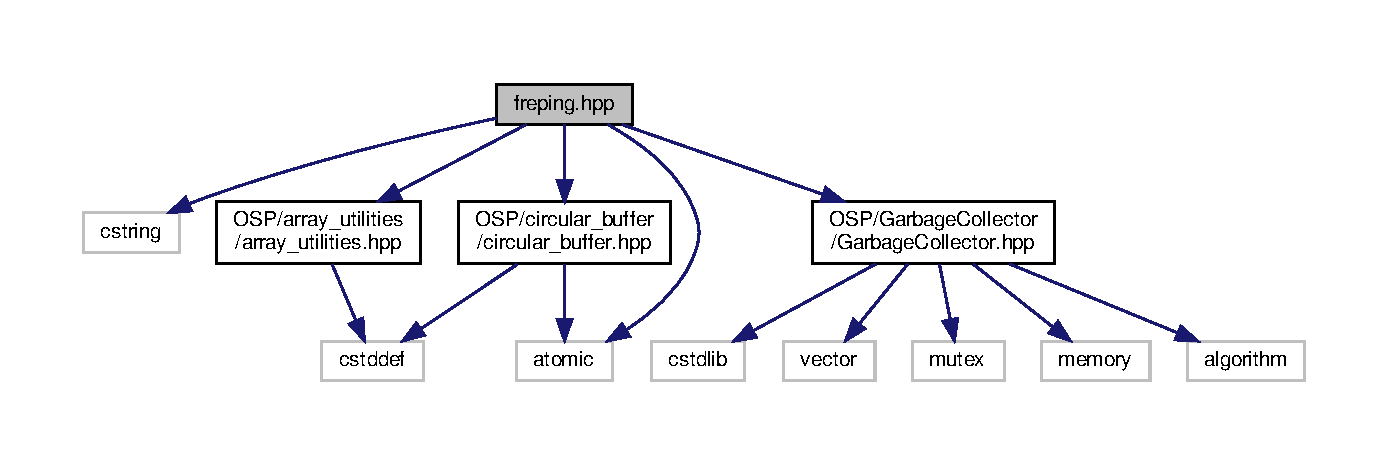
\includegraphics[width=350pt]{freping_8hpp__incl}
\end{center}
\end{figure}
This graph shows which files directly or indirectly include this file\+:\nopagebreak
\begin{figure}[H]
\begin{center}
\leavevmode
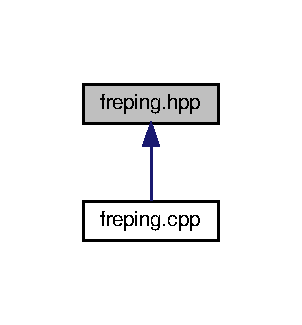
\includegraphics[width=145pt]{freping_8hpp__dep__incl}
\end{center}
\end{figure}
\subsection*{Classes}
\begin{DoxyCompactItemize}
\item 
class \hyperlink{classfreping}{freping}
\begin{DoxyCompactList}\small\item\em Freping Class. \end{DoxyCompactList}\end{DoxyCompactItemize}


\subsection{Detailed Description}
\begin{DoxyAuthor}{Author}
Open Speech Platform (O\+SP) Team, U\+C\+SD 
\end{DoxyAuthor}
\begin{DoxyCopyright}{Copyright}
Copyright (C) 2020 Regents of the University of California Redistribution and use in source and binary forms, with or without modification, are permitted provided that the following conditions are met\+: \begin{DoxyVerb}1. Redistributions of source code must retain the above copyright notice, this list of conditions and the
following disclaimer.

2. Redistributions in binary form must reproduce the above copyright notice, this list of conditions and the
following disclaimer in the documentation and/or other materials provided with the distribution.
\end{DoxyVerb}

\end{DoxyCopyright}
T\+H\+IS S\+O\+F\+T\+W\+A\+RE IS P\+R\+O\+V\+I\+D\+ED BY T\+HE C\+O\+P\+Y\+R\+I\+G\+HT H\+O\+L\+D\+E\+RS A\+ND C\+O\+N\+T\+R\+I\+B\+U\+T\+O\+RS \char`\"{}\+A\+S I\+S\char`\"{} A\+ND A\+NY E\+X\+P\+R\+E\+SS OR I\+M\+P\+L\+I\+ED W\+A\+R\+R\+A\+N\+T\+I\+ES, I\+N\+C\+L\+U\+D\+I\+NG, B\+UT N\+OT L\+I\+M\+I\+T\+ED TO, T\+HE I\+M\+P\+L\+I\+ED W\+A\+R\+R\+A\+N\+T\+I\+ES OF M\+E\+R\+C\+H\+A\+N\+T\+A\+B\+I\+L\+I\+TY A\+ND F\+I\+T\+N\+E\+SS F\+OR A P\+A\+R\+T\+I\+C\+U\+L\+AR P\+U\+R\+P\+O\+SE A\+RE D\+I\+S\+C\+L\+A\+I\+M\+ED. IN NO E\+V\+E\+NT S\+H\+A\+LL T\+HE C\+O\+P\+Y\+R\+I\+G\+HT H\+O\+L\+D\+ER OR C\+O\+N\+T\+R\+I\+B\+U\+T\+O\+RS BE L\+I\+A\+B\+LE F\+OR A\+NY D\+I\+R\+E\+CT, I\+N\+D\+I\+R\+E\+CT, I\+N\+C\+I\+D\+E\+N\+T\+AL, S\+P\+E\+C\+I\+AL, E\+X\+E\+M\+P\+L\+A\+RY, OR C\+O\+N\+S\+E\+Q\+U\+E\+N\+T\+I\+AL D\+A\+M\+A\+G\+ES (I\+N\+C\+L\+U\+D\+I\+NG, B\+UT N\+OT L\+I\+M\+I\+T\+ED TO, P\+R\+O\+C\+U\+R\+E\+M\+E\+NT OF S\+U\+B\+S\+T\+I\+T\+U\+TE G\+O\+O\+DS OR S\+E\+R\+V\+I\+C\+ES; L\+O\+SS OF U\+SE, D\+A\+TA, OR P\+R\+O\+F\+I\+TS; OR B\+U\+S\+I\+N\+E\+SS I\+N\+T\+E\+R\+R\+U\+P\+T\+I\+ON) H\+O\+W\+E\+V\+ER C\+A\+U\+S\+ED A\+ND ON A\+NY T\+H\+E\+O\+RY OF L\+I\+A\+B\+I\+L\+I\+TY, W\+H\+E\+T\+H\+ER IN C\+O\+N\+T\+R\+A\+CT, S\+T\+R\+I\+CT L\+I\+A\+B\+I\+L\+I\+TY, OR T\+O\+RT (I\+N\+C\+L\+U\+D\+I\+NG N\+E\+G\+L\+I\+G\+E\+N\+CE OR O\+T\+H\+E\+R\+W\+I\+SE) A\+R\+I\+S\+I\+NG IN A\+NY W\+AY O\+UT OF T\+HE U\+SE OF T\+H\+IS S\+O\+F\+T\+W\+A\+RE, E\+V\+EN IF A\+D\+V\+I\+S\+ED OF T\+HE P\+O\+S\+S\+I\+B\+I\+L\+I\+TY OF S\+U\+CH D\+A\+M\+A\+GE. 
\hypertarget{hamming__window128_8h}{}\section{hamming\+\_\+window128.\+h File Reference}
\label{hamming__window128_8h}\index{hamming\+\_\+window128.\+h@{hamming\+\_\+window128.\+h}}
\subsection*{Variables}
\begin{DoxyCompactItemize}
\item 
\mbox{\Hypertarget{hamming__window128_8h_a2704f1fd3864e891384ca50fd71a6502}\label{hamming__window128_8h_a2704f1fd3864e891384ca50fd71a6502}} 
long {\bfseries hamming\+\_\+window128\+\_\+length} = 128
\end{DoxyCompactItemize}


\subsection{Detailed Description}
\begin{DoxyAuthor}{Author}
Open Speech Platform (O\+SP) Team, U\+C\+SD 
\end{DoxyAuthor}
\begin{DoxyCopyright}{Copyright}
Copyright (C) 2020 Regents of the University of California Redistribution and use in source and binary forms, with or without modification, are permitted provided that the following conditions are met\+: \begin{DoxyVerb}1. Redistributions of source code must retain the above copyright notice, this list of conditions and the
following disclaimer.

2. Redistributions in binary form must reproduce the above copyright notice, this list of conditions and the
following disclaimer in the documentation and/or other materials provided with the distribution.
\end{DoxyVerb}

\end{DoxyCopyright}
T\+H\+IS S\+O\+F\+T\+W\+A\+RE IS P\+R\+O\+V\+I\+D\+ED BY T\+HE C\+O\+P\+Y\+R\+I\+G\+HT H\+O\+L\+D\+E\+RS A\+ND C\+O\+N\+T\+R\+I\+B\+U\+T\+O\+RS \char`\"{}\+A\+S I\+S\char`\"{} A\+ND A\+NY E\+X\+P\+R\+E\+SS OR I\+M\+P\+L\+I\+ED W\+A\+R\+R\+A\+N\+T\+I\+ES, I\+N\+C\+L\+U\+D\+I\+NG, B\+UT N\+OT L\+I\+M\+I\+T\+ED TO, T\+HE I\+M\+P\+L\+I\+ED W\+A\+R\+R\+A\+N\+T\+I\+ES OF M\+E\+R\+C\+H\+A\+N\+T\+A\+B\+I\+L\+I\+TY A\+ND F\+I\+T\+N\+E\+SS F\+OR A P\+A\+R\+T\+I\+C\+U\+L\+AR P\+U\+R\+P\+O\+SE A\+RE D\+I\+S\+C\+L\+A\+I\+M\+ED. IN NO E\+V\+E\+NT S\+H\+A\+LL T\+HE C\+O\+P\+Y\+R\+I\+G\+HT H\+O\+L\+D\+ER OR C\+O\+N\+T\+R\+I\+B\+U\+T\+O\+RS BE L\+I\+A\+B\+LE F\+OR A\+NY D\+I\+R\+E\+CT, I\+N\+D\+I\+R\+E\+CT, I\+N\+C\+I\+D\+E\+N\+T\+AL, S\+P\+E\+C\+I\+AL, E\+X\+E\+M\+P\+L\+A\+RY, OR C\+O\+N\+S\+E\+Q\+U\+E\+N\+T\+I\+AL D\+A\+M\+A\+G\+ES (I\+N\+C\+L\+U\+D\+I\+NG, B\+UT N\+OT L\+I\+M\+I\+T\+ED TO, P\+R\+O\+C\+U\+R\+E\+M\+E\+NT OF S\+U\+B\+S\+T\+I\+T\+U\+TE G\+O\+O\+DS OR S\+E\+R\+V\+I\+C\+ES; L\+O\+SS OF U\+SE, D\+A\+TA, OR P\+R\+O\+F\+I\+TS; OR B\+U\+S\+I\+N\+E\+SS I\+N\+T\+E\+R\+R\+U\+P\+T\+I\+ON) H\+O\+W\+E\+V\+ER C\+A\+U\+S\+ED A\+ND ON A\+NY T\+H\+E\+O\+RY OF L\+I\+A\+B\+I\+L\+I\+TY, W\+H\+E\+T\+H\+ER IN C\+O\+N\+T\+R\+A\+CT, S\+T\+R\+I\+CT L\+I\+A\+B\+I\+L\+I\+TY, OR T\+O\+RT (I\+N\+C\+L\+U\+D\+I\+NG N\+E\+G\+L\+I\+G\+E\+N\+CE OR O\+T\+H\+E\+R\+W\+I\+SE) A\+R\+I\+S\+I\+NG IN A\+NY W\+AY O\+UT OF T\+HE U\+SE OF T\+H\+IS S\+O\+F\+T\+W\+A\+RE, E\+V\+EN IF A\+D\+V\+I\+S\+ED OF T\+HE P\+O\+S\+S\+I\+B\+I\+L\+I\+TY OF S\+U\+CH D\+A\+M\+A\+GE. 
\hypertarget{hamming__window64_8h}{}\section{hamming\+\_\+window64.\+h File Reference}
\label{hamming__window64_8h}\index{hamming\+\_\+window64.\+h@{hamming\+\_\+window64.\+h}}
\subsection*{Variables}
\begin{DoxyCompactItemize}
\item 
\mbox{\Hypertarget{hamming__window64_8h_a8aea4117ab96a4e443139590b32f3a8f}\label{hamming__window64_8h_a8aea4117ab96a4e443139590b32f3a8f}} 
long {\bfseries hamming\+\_\+window64\+\_\+length} = 64
\end{DoxyCompactItemize}


\subsection{Detailed Description}
\begin{DoxyAuthor}{Author}
Open Speech Platform (O\+SP) Team, U\+C\+SD 
\end{DoxyAuthor}
\begin{DoxyCopyright}{Copyright}
Copyright (C) 2020 Regents of the University of California Redistribution and use in source and binary forms, with or without modification, are permitted provided that the following conditions are met\+: \begin{DoxyVerb}1. Redistributions of source code must retain the above copyright notice, this list of conditions and the
following disclaimer.

2. Redistributions in binary form must reproduce the above copyright notice, this list of conditions and the
following disclaimer in the documentation and/or other materials provided with the distribution.
\end{DoxyVerb}

\end{DoxyCopyright}
T\+H\+IS S\+O\+F\+T\+W\+A\+RE IS P\+R\+O\+V\+I\+D\+ED BY T\+HE C\+O\+P\+Y\+R\+I\+G\+HT H\+O\+L\+D\+E\+RS A\+ND C\+O\+N\+T\+R\+I\+B\+U\+T\+O\+RS \char`\"{}\+A\+S I\+S\char`\"{} A\+ND A\+NY E\+X\+P\+R\+E\+SS OR I\+M\+P\+L\+I\+ED W\+A\+R\+R\+A\+N\+T\+I\+ES, I\+N\+C\+L\+U\+D\+I\+NG, B\+UT N\+OT L\+I\+M\+I\+T\+ED TO, T\+HE I\+M\+P\+L\+I\+ED W\+A\+R\+R\+A\+N\+T\+I\+ES OF M\+E\+R\+C\+H\+A\+N\+T\+A\+B\+I\+L\+I\+TY A\+ND F\+I\+T\+N\+E\+SS F\+OR A P\+A\+R\+T\+I\+C\+U\+L\+AR P\+U\+R\+P\+O\+SE A\+RE D\+I\+S\+C\+L\+A\+I\+M\+ED. IN NO E\+V\+E\+NT S\+H\+A\+LL T\+HE C\+O\+P\+Y\+R\+I\+G\+HT H\+O\+L\+D\+ER OR C\+O\+N\+T\+R\+I\+B\+U\+T\+O\+RS BE L\+I\+A\+B\+LE F\+OR A\+NY D\+I\+R\+E\+CT, I\+N\+D\+I\+R\+E\+CT, I\+N\+C\+I\+D\+E\+N\+T\+AL, S\+P\+E\+C\+I\+AL, E\+X\+E\+M\+P\+L\+A\+RY, OR C\+O\+N\+S\+E\+Q\+U\+E\+N\+T\+I\+AL D\+A\+M\+A\+G\+ES (I\+N\+C\+L\+U\+D\+I\+NG, B\+UT N\+OT L\+I\+M\+I\+T\+ED TO, P\+R\+O\+C\+U\+R\+E\+M\+E\+NT OF S\+U\+B\+S\+T\+I\+T\+U\+TE G\+O\+O\+DS OR S\+E\+R\+V\+I\+C\+ES; L\+O\+SS OF U\+SE, D\+A\+TA, OR P\+R\+O\+F\+I\+TS; OR B\+U\+S\+I\+N\+E\+SS I\+N\+T\+E\+R\+R\+U\+P\+T\+I\+ON) H\+O\+W\+E\+V\+ER C\+A\+U\+S\+ED A\+ND ON A\+NY T\+H\+E\+O\+RY OF L\+I\+A\+B\+I\+L\+I\+TY, W\+H\+E\+T\+H\+ER IN C\+O\+N\+T\+R\+A\+CT, S\+T\+R\+I\+CT L\+I\+A\+B\+I\+L\+I\+TY, OR T\+O\+RT (I\+N\+C\+L\+U\+D\+I\+NG N\+E\+G\+L\+I\+G\+E\+N\+CE OR O\+T\+H\+E\+R\+W\+I\+SE) A\+R\+I\+S\+I\+NG IN A\+NY W\+AY O\+UT OF T\+HE U\+SE OF T\+H\+IS S\+O\+F\+T\+W\+A\+RE, E\+V\+EN IF A\+D\+V\+I\+S\+ED OF T\+HE P\+O\+S\+S\+I\+B\+I\+L\+I\+TY OF S\+U\+CH D\+A\+M\+A\+GE. 
\hypertarget{prefilter_8h}{}\section{prefilter.\+h File Reference}
\label{prefilter_8h}\index{prefilter.\+h@{prefilter.\+h}}
\subsection*{Macros}
\begin{DoxyCompactItemize}
\item 
\mbox{\Hypertarget{prefilter_8h_ad950490c70c49d4c15a2f6c69f6a7969}\label{prefilter_8h_ad950490c70c49d4c15a2f6c69f6a7969}} 
\#define {\bfseries P\+R\+E\+F\+I\+L\+T\+E\+R\+\_\+\+S\+I\+ZE}~3
\end{DoxyCompactItemize}
\subsection*{Variables}
\begin{DoxyCompactItemize}
\item 
float {\bfseries prefilter} \mbox{[}P\+R\+E\+F\+I\+L\+T\+E\+R\+\_\+\+S\+I\+ZE\mbox{]}
\end{DoxyCompactItemize}


\subsection{Detailed Description}
\begin{DoxyAuthor}{Author}
Open Speech Platform (O\+SP) Team, U\+C\+SD 
\end{DoxyAuthor}
\begin{DoxyCopyright}{Copyright}
Copyright (C) 2020 Regents of the University of California Redistribution and use in source and binary forms, with or without modification, are permitted provided that the following conditions are met\+: \begin{DoxyVerb}1. Redistributions of source code must retain the above copyright notice, this list of conditions and the
following disclaimer.

2. Redistributions in binary form must reproduce the above copyright notice, this list of conditions and the
following disclaimer in the documentation and/or other materials provided with the distribution.
\end{DoxyVerb}

\end{DoxyCopyright}
T\+H\+IS S\+O\+F\+T\+W\+A\+RE IS P\+R\+O\+V\+I\+D\+ED BY T\+HE C\+O\+P\+Y\+R\+I\+G\+HT H\+O\+L\+D\+E\+RS A\+ND C\+O\+N\+T\+R\+I\+B\+U\+T\+O\+RS \char`\"{}\+A\+S I\+S\char`\"{} A\+ND A\+NY E\+X\+P\+R\+E\+SS OR I\+M\+P\+L\+I\+ED W\+A\+R\+R\+A\+N\+T\+I\+ES, I\+N\+C\+L\+U\+D\+I\+NG, B\+UT N\+OT L\+I\+M\+I\+T\+ED TO, T\+HE I\+M\+P\+L\+I\+ED W\+A\+R\+R\+A\+N\+T\+I\+ES OF M\+E\+R\+C\+H\+A\+N\+T\+A\+B\+I\+L\+I\+TY A\+ND F\+I\+T\+N\+E\+SS F\+OR A P\+A\+R\+T\+I\+C\+U\+L\+AR P\+U\+R\+P\+O\+SE A\+RE D\+I\+S\+C\+L\+A\+I\+M\+ED. IN NO E\+V\+E\+NT S\+H\+A\+LL T\+HE C\+O\+P\+Y\+R\+I\+G\+HT H\+O\+L\+D\+ER OR C\+O\+N\+T\+R\+I\+B\+U\+T\+O\+RS BE L\+I\+A\+B\+LE F\+OR A\+NY D\+I\+R\+E\+CT, I\+N\+D\+I\+R\+E\+CT, I\+N\+C\+I\+D\+E\+N\+T\+AL, S\+P\+E\+C\+I\+AL, E\+X\+E\+M\+P\+L\+A\+RY, OR C\+O\+N\+S\+E\+Q\+U\+E\+N\+T\+I\+AL D\+A\+M\+A\+G\+ES (I\+N\+C\+L\+U\+D\+I\+NG, B\+UT N\+OT L\+I\+M\+I\+T\+ED TO, P\+R\+O\+C\+U\+R\+E\+M\+E\+NT OF S\+U\+B\+S\+T\+I\+T\+U\+TE G\+O\+O\+DS OR S\+E\+R\+V\+I\+C\+ES; L\+O\+SS OF U\+SE, D\+A\+TA, OR P\+R\+O\+F\+I\+TS; OR B\+U\+S\+I\+N\+E\+SS I\+N\+T\+E\+R\+R\+U\+P\+T\+I\+ON) H\+O\+W\+E\+V\+ER C\+A\+U\+S\+ED A\+ND ON A\+NY T\+H\+E\+O\+RY OF L\+I\+A\+B\+I\+L\+I\+TY, W\+H\+E\+T\+H\+ER IN C\+O\+N\+T\+R\+A\+CT, S\+T\+R\+I\+CT L\+I\+A\+B\+I\+L\+I\+TY, OR T\+O\+RT (I\+N\+C\+L\+U\+D\+I\+NG N\+E\+G\+L\+I\+G\+E\+N\+CE OR O\+T\+H\+E\+R\+W\+I\+SE) A\+R\+I\+S\+I\+NG IN A\+NY W\+AY O\+UT OF T\+HE U\+SE OF T\+H\+IS S\+O\+F\+T\+W\+A\+RE, E\+V\+EN IF A\+D\+V\+I\+S\+ED OF T\+HE P\+O\+S\+S\+I\+B\+I\+L\+I\+TY OF S\+U\+CH D\+A\+M\+A\+GE. 

\subsection{Variable Documentation}
\mbox{\Hypertarget{prefilter_8h_a7688ebc3a90806de8e7f9cfc4f3ffd75}\label{prefilter_8h_a7688ebc3a90806de8e7f9cfc4f3ffd75}} 
\index{prefilter.\+h@{prefilter.\+h}!prefilter@{prefilter}}
\index{prefilter@{prefilter}!prefilter.\+h@{prefilter.\+h}}
\subsubsection{\texorpdfstring{prefilter}{prefilter}}
{\footnotesize\ttfamily float prefilter\mbox{[}P\+R\+E\+F\+I\+L\+T\+E\+R\+\_\+\+S\+I\+ZE\mbox{]}}

{\bfseries Initial value\+:}
\begin{DoxyCode}
= \{
        1.0f,
        -2.01f,
        1.0f
\}
\end{DoxyCode}


Definition at line 32 of file prefilter.\+h.


\hypertarget{sokolovaharris__filtercoef_8h}{}\section{sokolovaharris\+\_\+filtercoef.\+h File Reference}
\label{sokolovaharris__filtercoef_8h}\index{sokolovaharris\+\_\+filtercoef.\+h@{sokolovaharris\+\_\+filtercoef.\+h}}
{\ttfamily \#include $<$cstddef$>$}\newline
{\ttfamily \#include \char`\"{}tenband\+\_\+filterbank.\+h\char`\"{}}\newline
Include dependency graph for sokolovaharris\+\_\+filtercoef.\+h\+:\nopagebreak
\begin{figure}[H]
\begin{center}
\leavevmode
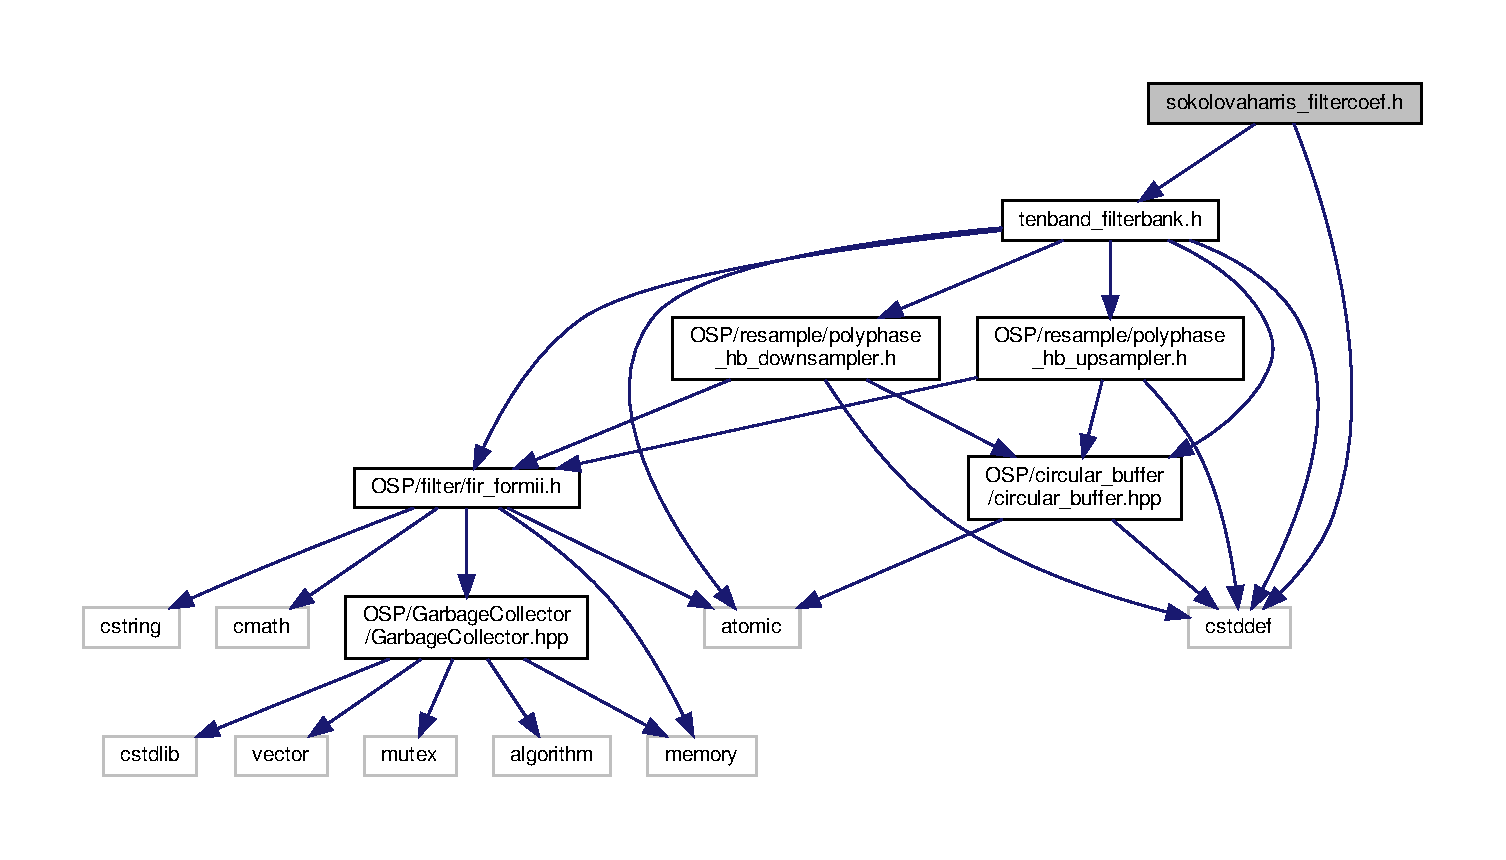
\includegraphics[width=350pt]{sokolovaharris__filtercoef_8h__incl}
\end{center}
\end{figure}
This graph shows which files directly or indirectly include this file\+:\nopagebreak
\begin{figure}[H]
\begin{center}
\leavevmode
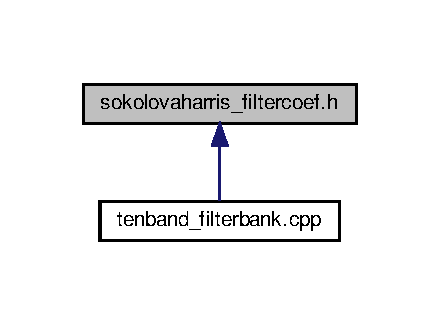
\includegraphics[width=211pt]{sokolovaharris__filtercoef_8h__dep__incl}
\end{center}
\end{figure}
\subsection*{Variables}
\begin{DoxyCompactItemize}
\item 
\mbox{\Hypertarget{sokolovaharris__filtercoef_8h_ae61251ecaad415aa0fe848b346565efe}\label{sokolovaharris__filtercoef_8h_ae61251ecaad415aa0fe848b346565efe}} 
size\+\_\+t {\bfseries half\+\_\+band\+\_\+filter1\+\_\+length} = 35
\item 
\mbox{\Hypertarget{sokolovaharris__filtercoef_8h_ad3ca1a0cecf0804d63a296311fdf2727}\label{sokolovaharris__filtercoef_8h_ad3ca1a0cecf0804d63a296311fdf2727}} 
size\+\_\+t {\bfseries half\+\_\+band\+\_\+filter2\+\_\+length} = 11
\item 
\mbox{\Hypertarget{sokolovaharris__filtercoef_8h_a5f2d72b6530dd1887495b5ba2dcd544f}\label{sokolovaharris__filtercoef_8h_a5f2d72b6530dd1887495b5ba2dcd544f}} 
size\+\_\+t {\bfseries half\+\_\+band\+\_\+filter3\+\_\+length} = 7
\end{DoxyCompactItemize}


\subsection{Detailed Description}
\begin{DoxyAuthor}{Author}
Open Speech Platform (O\+SP) Team, U\+C\+SD 
\end{DoxyAuthor}
\begin{DoxyCopyright}{Copyright}
Copyright (C) 2020 Regents of the University of California Redistribution and use in source and binary forms, with or without modification, are permitted provided that the following conditions are met\+: \begin{DoxyVerb}1. Redistributions of source code must retain the above copyright notice, this list of conditions and the
following disclaimer.

2. Redistributions in binary form must reproduce the above copyright notice, this list of conditions and the
following disclaimer in the documentation and/or other materials provided with the distribution.
\end{DoxyVerb}

\end{DoxyCopyright}
T\+H\+IS S\+O\+F\+T\+W\+A\+RE IS P\+R\+O\+V\+I\+D\+ED BY T\+HE C\+O\+P\+Y\+R\+I\+G\+HT H\+O\+L\+D\+E\+RS A\+ND C\+O\+N\+T\+R\+I\+B\+U\+T\+O\+RS \char`\"{}\+A\+S I\+S\char`\"{} A\+ND A\+NY E\+X\+P\+R\+E\+SS OR I\+M\+P\+L\+I\+ED W\+A\+R\+R\+A\+N\+T\+I\+ES, I\+N\+C\+L\+U\+D\+I\+NG, B\+UT N\+OT L\+I\+M\+I\+T\+ED TO, T\+HE I\+M\+P\+L\+I\+ED W\+A\+R\+R\+A\+N\+T\+I\+ES OF M\+E\+R\+C\+H\+A\+N\+T\+A\+B\+I\+L\+I\+TY A\+ND F\+I\+T\+N\+E\+SS F\+OR A P\+A\+R\+T\+I\+C\+U\+L\+AR P\+U\+R\+P\+O\+SE A\+RE D\+I\+S\+C\+L\+A\+I\+M\+ED. IN NO E\+V\+E\+NT S\+H\+A\+LL T\+HE C\+O\+P\+Y\+R\+I\+G\+HT H\+O\+L\+D\+ER OR C\+O\+N\+T\+R\+I\+B\+U\+T\+O\+RS BE L\+I\+A\+B\+LE F\+OR A\+NY D\+I\+R\+E\+CT, I\+N\+D\+I\+R\+E\+CT, I\+N\+C\+I\+D\+E\+N\+T\+AL, S\+P\+E\+C\+I\+AL, E\+X\+E\+M\+P\+L\+A\+RY, OR C\+O\+N\+S\+E\+Q\+U\+E\+N\+T\+I\+AL D\+A\+M\+A\+G\+ES (I\+N\+C\+L\+U\+D\+I\+NG, B\+UT N\+OT L\+I\+M\+I\+T\+ED TO, P\+R\+O\+C\+U\+R\+E\+M\+E\+NT OF S\+U\+B\+S\+T\+I\+T\+U\+TE G\+O\+O\+DS OR S\+E\+R\+V\+I\+C\+ES; L\+O\+SS OF U\+SE, D\+A\+TA, OR P\+R\+O\+F\+I\+TS; OR B\+U\+S\+I\+N\+E\+SS I\+N\+T\+E\+R\+R\+U\+P\+T\+I\+ON) H\+O\+W\+E\+V\+ER C\+A\+U\+S\+ED A\+ND ON A\+NY T\+H\+E\+O\+RY OF L\+I\+A\+B\+I\+L\+I\+TY, W\+H\+E\+T\+H\+ER IN C\+O\+N\+T\+R\+A\+CT, S\+T\+R\+I\+CT L\+I\+A\+B\+I\+L\+I\+TY, OR T\+O\+RT (I\+N\+C\+L\+U\+D\+I\+NG N\+E\+G\+L\+I\+G\+E\+N\+CE OR O\+T\+H\+E\+R\+W\+I\+SE) A\+R\+I\+S\+I\+NG IN A\+NY W\+AY O\+UT OF T\+HE U\+SE OF T\+H\+IS S\+O\+F\+T\+W\+A\+RE, E\+V\+EN IF A\+D\+V\+I\+S\+ED OF T\+HE P\+O\+S\+S\+I\+B\+I\+L\+I\+TY OF S\+U\+CH D\+A\+M\+A\+GE. 
%--- End generated contents ---

% Index
\backmatter
\newpage
\phantomsection
\clearemptydoublepage
\addcontentsline{toc}{chapter}{Index}
\printindex

\end{document}
